\documentclass[oneside]{book}

\usepackage{NeededPackages}

\usepackage{import}

\usepackage{titlesec}
\titleformat{\chapter}[hang] 
{\centering \normalfont\Huge\bfseries}{}{1em}{} 




\title{\Huge \textbf{ATmega328P}}
\author{\textbf{Narendiran S}}
\date{\today}

\begin{document}

\maketitle

\tableofcontents

% \mainmatter
\chapter{Atmega328P Basics}
% \documentclass{article}
% \usepackage{NeededPackages}
% \title{ATmega328P Basics}
% \author{Narendiran S}
% \date{\today}

% \begin{document}
% \maketitle

\section{Features}
\begin{itemize}
    \item 8 bit CMOS $\mu$C with RISC Architecture
    \item 32 x 8-bit General purpose registers
    \item 32 KByte of flash program memory
    \item 1 KByte EEPROM
    \item 2 KByte of internal SRAM
    \item On-chip 2-cycle multiplier
    \item Optional boot code section with independent lock bits
    \begin{itemize}
        \item In-system programming by on-chip boot program
        \item True read-while-write operation
    \end{itemize}
    \item Two 8-bit Timer/Counter with  separate prescaler and compare mode
    \item One 16-bit Timer/Counter with  separate prescaler, compare mode and capture mode
    \item Real time counter with separate oscillator
    \item Six PWM channels
    \item 6/8(DEPENDING ON PACKAGE) chaneel 10 bit ADC 
        ◦ Also with Temperature measurement
    \item Programmable serial USART
    \item 2-wire serial interface (Phillips I2C compatible)
    \item Programmable watchdog timer with separate on-chip oscillator
    \item On-chip analog comparator
    \item Interrupt and wake-up on pin change
    \item Power-on reset and programmable brown-out detection
    \item External and internal interrupt sources
    \item Six sleep modes: Idle, ADC noise reduction, power-save, power-down, standby  and external standby
    \item 2.7V to 5.5V for ATmega328P
\end{itemize}

\newpage
\section{Block Diagram}
\begin{figure}[H]
    \centering
    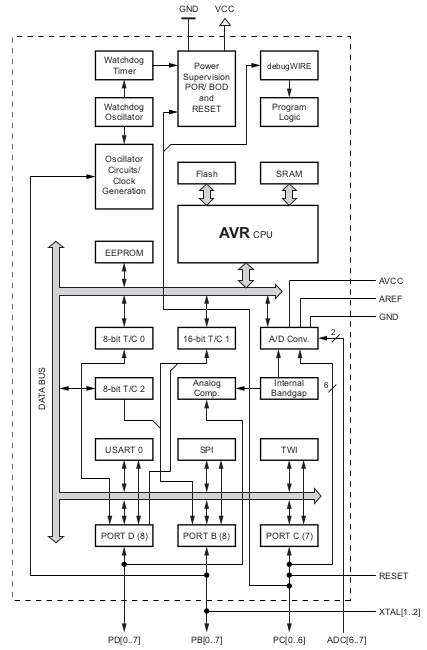
\includegraphics{blockDiagram.png}
\end{figure}

\newpage
\section{Pins}
\subsection{Power Pins}
\quad VCC, Gnd - 2.7V to 5.5V

\subsection{PORTB - PB7:PB0}
\begin{itemize}
    \item Bidirection I/O with internal pull-up resistor(selectable for each bit)
    \item Tristate when reset
    \item Depending on the clock selection fuse settings,
    \begin{itemize}
        \item \pinFormat{PB6} – input of inverting oscillator amplifier and input to internal clock operating circuit
        \item \pinFormat{PB7} – output of inverting oscillator amplifier
    \end{itemize}
    \item If internal calibrated RC oscillator is used as clock source, \pinFormat{PB7} and \pinFormat{PB6} is used as \pinFormat{TOSC2} and \pinFormat{TOSC1} input for Timer/Counter2
\end{itemize}

\subsection{PORTC - PC5:PB0}
\begin{itemize}
    \item Bidirection I/O with internal pull-up resistor(selectable for each bit)
    \item Tristate when reset
\end{itemize}

\subsection{PC6/\texorpdfstring{$\overline{RESET}$}{}}
\begin{itemize}
    \item Low level on this pin will gnerate reset, even if no clock running.
    \item \bitFormat{RSTDIBL} fuse == programmed(0) -- \pinFormat{PC6} is input pin.
    \item \bitFormat{RSTDIBL} fuse == unprogrammed(1) -- \pinFormat{PC6} is reset pin.
\end{itemize}

\subsection{PORTD - PD7:PD0}
\begin{itemize}
    \item Bidirection I/O with internal pull-up resistor(selectable for each bit)
    \item Tristate when reset
\end{itemize}

\subsection{\texorpdfstring{$AV_{CC}$}{}}
\begin{itemize}
    \item Supply voltage pin for A/D converter
    \item Connected to External Vcc when not used
    \item Connected to Vcc through LPF when used
\end{itemize}

\subsection{AREF}
\quad Analog reference pin of A/D Converter

\subsection{ADC7:ADC6}
\quad Analog input to ADC(10bit ADC)


\section{Modes}
\subsection{Idle Mode}
\quad Stops the CPU while allowing SRAM, TImer/Counters, USART, 2-wire serial interface, SPI port and interrupt system to continue functioning.

\subsection{Power-Down Mode}
\quad Saves the register contents but freezes the oscillator, disabling all other chip functions untill next interrupt or hardware reset.

\subsection{Power-Save Mode}
\quad The asynchonous timer continues to run, allowing user to maintain timer base while reset of devices is sleeping.

\subsection{ADC Noise reduction mode}
\quad Stops CPU and all I/O modules except asynchonous timer and ADC to minimize switching noise during ADC conversions.

\subsection{Standby Mode}
\quad The crystall/oscillator is running while reset of devices is sleeping. Allows very fast start-up combined with low power consumption.


\section{AVR CPU Core}
\quad The main function of CPU core is access memory, perform caluclations, control peripherals and handle interrupts.

\begin{figure}[H]
    \centering
    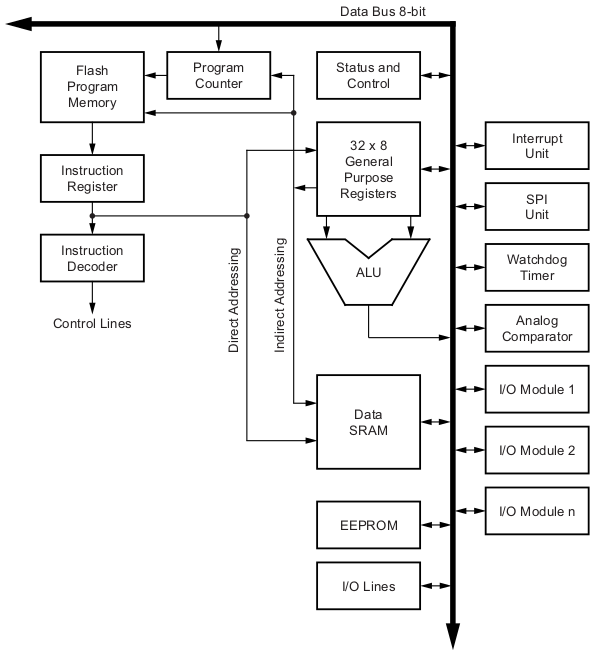
\includegraphics[height=0.7\textheight]{avrCoreBlockDiagram.png}
\end{figure}

\begin{itemize}
    \item For performance and parallelism, the AVR uses Harvard Architecture - with seperate memories and buses for program and data.
    \item Instructions in Program memory are exectued with a single level pipelining.
    \item The program memory is  \textbf{In-system Reprogrammable Flash memory}.
    \item The register file consist of 32 x 8-bit General Purpose Registers with a single clock cycle assess time.
    \item One ALU operation uses two operatands from register file and store back the result to register file in one clock cycle.
    \item Six 32-bit register combine to form the X-, Y- and Z- registers which help in 16-bit indirect address register pointer for data space.
    \item One of these pointers acts as address pointer for look-up tables in Flash Program Memory.
    \item Program memory adress cotains 16-bit or 32-bit Instructions.
    \item Program Flash memory space is divided into two sections - each section have dedicated lock bits for read/write protection.
    \begin{itemize}
        \item Boot Program section
        \item Application Program section
    \end{itemize}
    \item I/O memory space contains 64 addresses for CPU peripheral functions as control register, SPI and Other I/O functionscan be accessed directly or through register file from 0x20 - 0x5F.
    \item Has extended I/O space from 0x60 - 0xFF in SRAM.
\end{itemize}

\subsection{Reset and Interrupt vectors}
\begin{itemize}
    \item Interrupts and reset vectors have seperate program vecotr in program memory space.
    \item Interrupts maye be disbaled when boot lock bits \bitFormat{BLB02} or \bitFormat{BLB12} are programmed.
    \item Lowest ddresses in program memory space are reset and interrupt vectors.
    \item The lower the addess the higher the priority.
    \item RESET has the highest followed by INT0(the external interrupt request 0).
    \item The interrupt vectors can be moved to start of boot flash section by setting \bitFormat{IVSEL} bit of \regFormat{MCUCR} (MCU control register).
    \item THe reset can be moved to start of boot flash sectio by programming the \bitFormat{BOOTRST} fuse.
\end{itemize}

\subsection{Interrupt Handling}
\begin{itemize}
    \item The \bitFormat{I-bit} (global interrupt enable bit) of \regFormat{Status register} must be enabled.
    \item When a interrupt occurs, \bitFormat{I-bit} (global interrupt enable bit) is cleared and all interrupts are disabled.
    \item The user can write logic one to \bitFormat{I-bit} to enable nested interrupts.
    \item The \bitFormat{I-bit} is automatically set when returning from interrupt Instructions.
\end{itemize}


\section{AVR Memories}
\quad Two main memory spaces - Data memory and Program memory space and a EEPROM memory for data storage.

\subsection{In-System Reprogrammable Flash Program Memory}
\begin{itemize}
    \item 32 KBytes on-chip in-system reprogrammable flash memory for program space.
    \item Since, the Instructions are all 16-bit or  32-bit wide, the flash(program space) is organized as 16K x 16.
    \item Endurance of atleast 10,000 write/erase cycle.
    \item For software security, Flash program memory space is divided into
    \begin{itemize}
        \item Boot Loaded section
        \item Application Program section
    \end{itemize}
    \item The Program Counter is bits wide and thus can address 16K program memory location.\end{itemize}

\begin{figure}[H]
    \begin{center}
        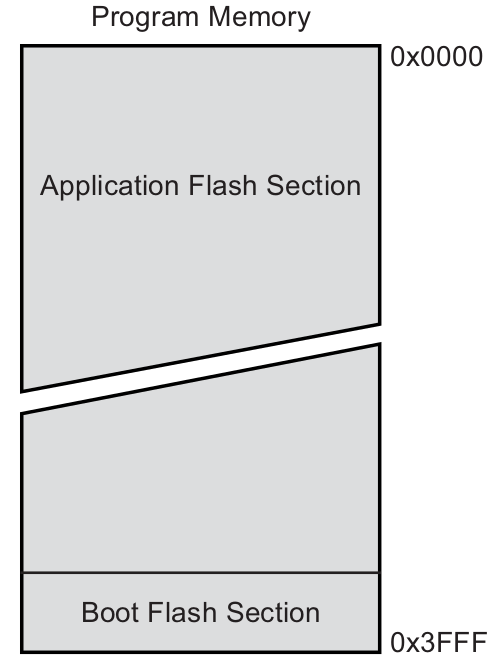
\includegraphics[height=0.27\textheight]{programMemoryFlash.png}
    \end{center}
\end{figure}

\subsection{SRAM Data Memory}
\begin{itemize}
    \item The ATmega328P is a complex microcontroller with more peripheral units than can be supported within the 64 locations reserved in the opcode for the IN and OUT instructions.
    \item For the extended I/O space from 0x60 - 0xFF in SRAM, only the ST/STS/STD and LD/LDS/LDD instructions can be used.
    \begin{figure}[H]
        \begin{center}
            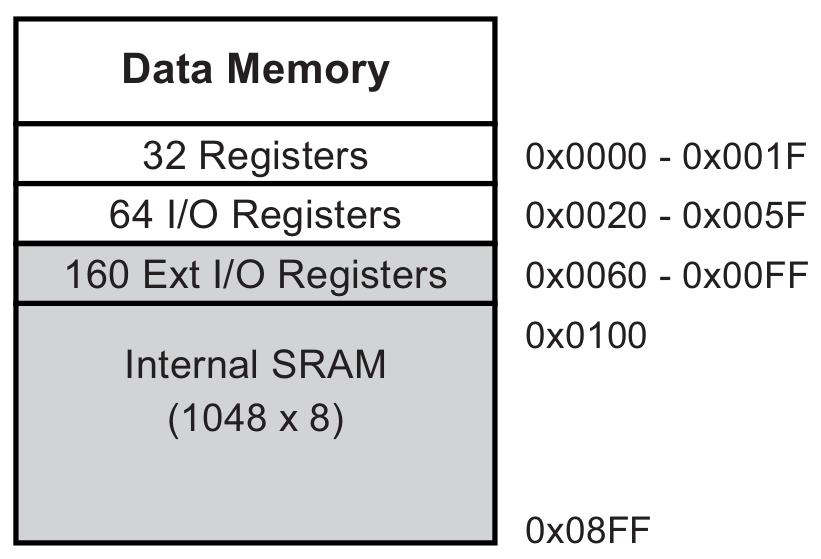
\includegraphics[height=0.25\textheight]{dataMemorySRAM.png}
        \end{center}
    \end{figure}
    \item The lower 2303(0x08FF) data memory locations addresses both the register files, the I/O memory, extended I/O memory and the internal data SRAM.
    \begin{itemize}
        \item The first 32 location addresses the register file.
        \item The next 64 location addresses the standard I/O memory.
        \item The following 160 location address the extended I"O memory.
        \item The last 2048 location address the internal data SRAM.
    \end{itemize}
\end{itemize}

\subsection{EEPROM Data Memory}
\begin{itemize}
    \item 1 K Byte of data EEPROM memory.
    \item Organized as seperate data space.
    \item Endurance of atleast 100,000 write/erase cycle.
    \item EEPROM are accessible in I/O space.
    \item Specific Write procedure is followed. 
\end{itemize}

\subsection{I/O Memory}
\begin{itemize}
    \item I/O and peripherals are placed in the I/O spaces.
    \item All I/O locations are accesed by LD/LDS/LDD and ST/STS/STD instructions.
    \item The I/O registers withing 0x00 - 0x1F are directly bit-accessible using SBI and CBI Instructions.
\end{itemize}


\section{System Clock and Clock Options}
\begin{figure}[H]
    \begin{center}
        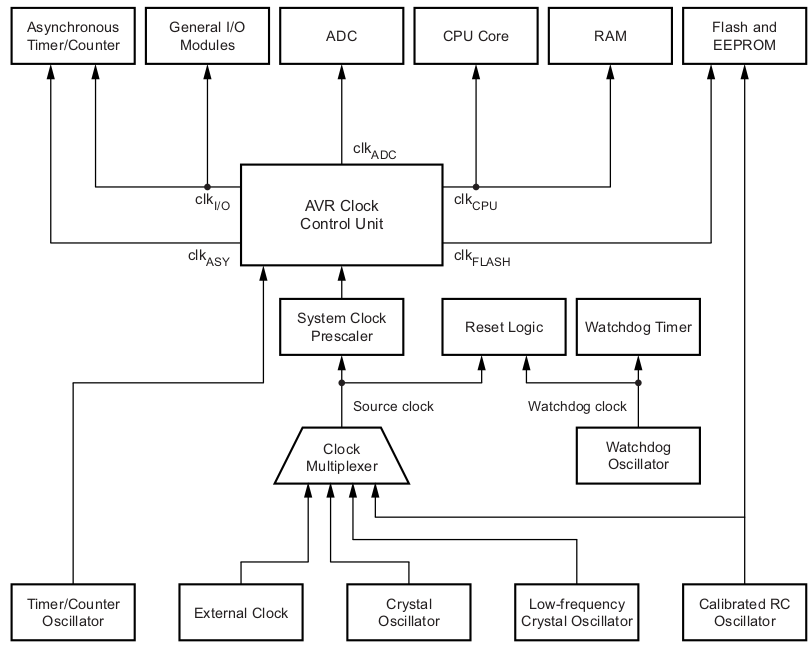
\includegraphics[height=0.5\textheight]{clkDistribution.png}
    \end{center}
\end{figure}

\subsection{Clock Systems}
\subsubsection{CPU Clock}
\begin{itemize}
    \item $clk_{CPU}$ is routed to all parts of AVR core.
    \item General purpose register file, Status register and data memory holding stack pointer.
    \item Halting CPU clock will inhibts the core from perfrorming general operations and caluclations.
\end{itemize}

\subsubsection{I/O Clock}
\begin{itemize}
    \item $clk_{I/O}$ is used in I/O modules like Timers/Counter, SPI, USART, etc.
    \item For external interrupt module also but some external interrupts are detected by asynchonous logic and can be used even when I/O clock is halted.
\end{itemize}

\subsubsection{Flash Clock}
\begin{itemize}
    \item $clk_{FLASH}$ controls operation of flash interface.
\end{itemize}


\subsubsection{Asynchronous Timer Clock}
\begin{itemize}
    \item $clk_{ASY}$ allows asynchonous Timer/Counter to be clocked directly from external clock or an external 32 kHz clock crystall.
    \item This clock allows using Timer/COunter as real-time counter even when device is in sleep mode.
\end{itemize}

\subsubsection{ADC Clock}
\begin{itemize}
    \item $clk_{ADC} had dedicated clock domain$
    \item Gives more accurate ADC conversion result
\end{itemize}

\subsection{Clock Sources}
\quad Selectable clock sources using flash fuse bits.

\begin{table}[H]
    \begin{center}
        \begin{tabular}{c|c}
            \textbf{\bitFormat{CKSEL[3:0]}} & \textbf{Device Clocking Option}\\
            \hline
            1111 - 1000 & Low power crystall oscillator\\
            0111 - 0110 & Full swing crystal oscillator\\
            0101 - 0100 & Low frequency crystal oscillator\\
            0011 & Internal 128kHz RC oscillator\\
            0010 & Calibrated internal RC oscillator\\
            0000 & External clock            
        \end{tabular}
    \end{center}
\end{table}

{\Large \textbf{For fuses, "1" denotes unprogrammed and "0" denotes programmed.}}

\subsubsection*{Default Clock Source}
\begin{itemize}
    \item Devices is shipped with interface RC oscillator at 8.0MHz with fuse \bitFormat{CKDIV8} programmed meaning $---->$ the internal oscillator produces a 8.0 Mhz clock but due to \bitFormat{CKDIV8} being programmed the system clock gets $\frac{8.0 MHz}{8} = 1 MHz$.
    \item The startup time is set to maximum and time-out period enabled.
    \item Default configuration $--->$ \bitFormat{CKSEL} = 0010; \bitFormat{SUT} = 10; \bitFormat{CKDIV8} = 0.
\end{itemize}

\subsubsection*{Clock Start Sequence}
\begin{itemize}
    \item Clock Source needs a sufficient $V_{CC}$ and minimum number of oscillating cycles before stablizing.
    \item To ensure sufficient $V_{CC}$, the device issues an internal reset with time-out delay ($t_{TOUT}$).
    \item The number of cyles in the dealy is set by \bitFormat{SUTx} bits and \bitFormat{CKSELx} fuse bits.
    \item The main purpose of dealy is to keep AVR in reset until it is supplied with minimal $V_{CC}$.
    \item The start-up sequence for the clock includes both the time-out delay and the start-up time when the device starts up from
    reset.
\end{itemize}

\subsubsection*{Clock Output Buffer}
\begin{itemize}
    \item device can output system clock on the \pinFormat{CLKO} pin.
    \item enabled by \pinFormat{CKOUT} fuse.
    \item any clock source can be used to output from this pin.
\end{itemize}

\subsubsection*{TIMER/COUNTER OSCILLATOR}
\begin{itemize}
    \item uses the same crystal oscillator for low-frequency oscillator and Timer/Counter oscillator.
    \item Since, It shares the Timer/Counter oscillator pins  \pinFormat{TOSC1} and \pinFormat{TOSC2} pins with \pinFormat{XTAL1} and \pinFormat{XTAL2}, the system clock must be four times the oscillator and so the Timer/Counter oscillator can only be used when the calibrated internal RC oscillator is selected as system clock source.
\end{itemize}

\subsubsection{Low Power Crystall OSscillator}

\begin{figure}[H]
	\begin{minipage}{.45\textwidth}
		\begin{center}
			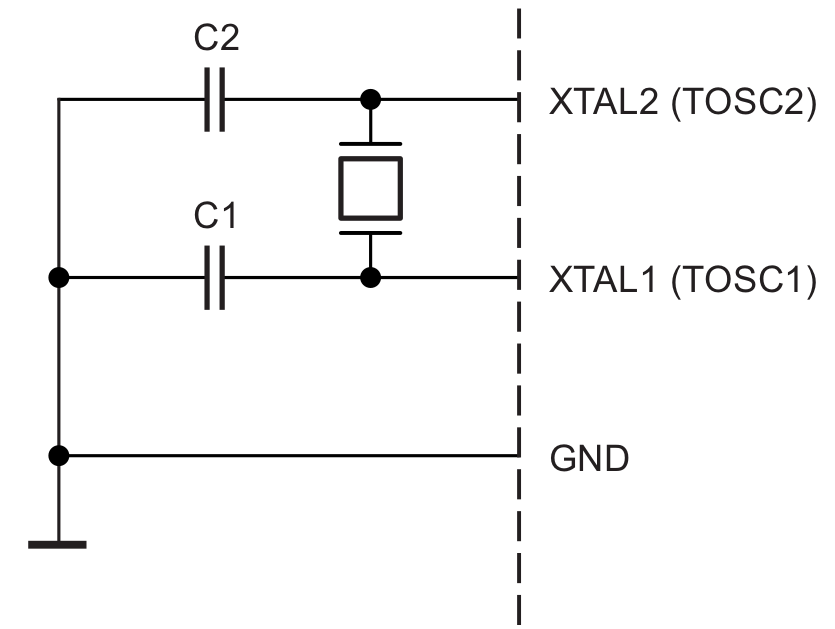
\includegraphics[width=0.45\textwidth]{lowPowerCrystallOscillatorCircuit.png}
			\caption{VGA Connector}
		\end{center}
	\end{minipage}
	\begin{minipage}{.5\textwidth}
		\begin{center}
			\begin{tabular}{c|c}
                \bitFormat{CKSEL[3:1]} & \textbf{Frequency Range (MHz)}\\
                \hline
                100 & 0.4 to 0.9(only Ceramic resonators)\\
                101 & 0.9 to 3.0\\
                110 & 3.0 to 8.0\\
                111 & 8.0 to 16.0\\
            \end{tabular}
		\end{center}
	\end{minipage}
\end{figure}


\begin{itemize}
    \item \pinFormat{XTAL1} and \pinFormat{XTAL2} are inputs and outpus of an inverting amplifier which can be configured as on-chip oscillator.
    \item Either Quartz Crystall or Ceramic resonator can be used.
    \item Crystal Oscillator is a low power oscillator with reduced voltage swing on the XTAL2 output.
    \item Not capable of driving other clock inputs.
    \item C1 and C2 should be of the same values – 12pF to 22pF.
    \item The \bitFormat{CKSEL[0]} fuse together with the \bitFormat{SUT[1:0]} fuses select the start-up times as shown in Table below.
    \begin{figure}[H]
        \begin{center}
            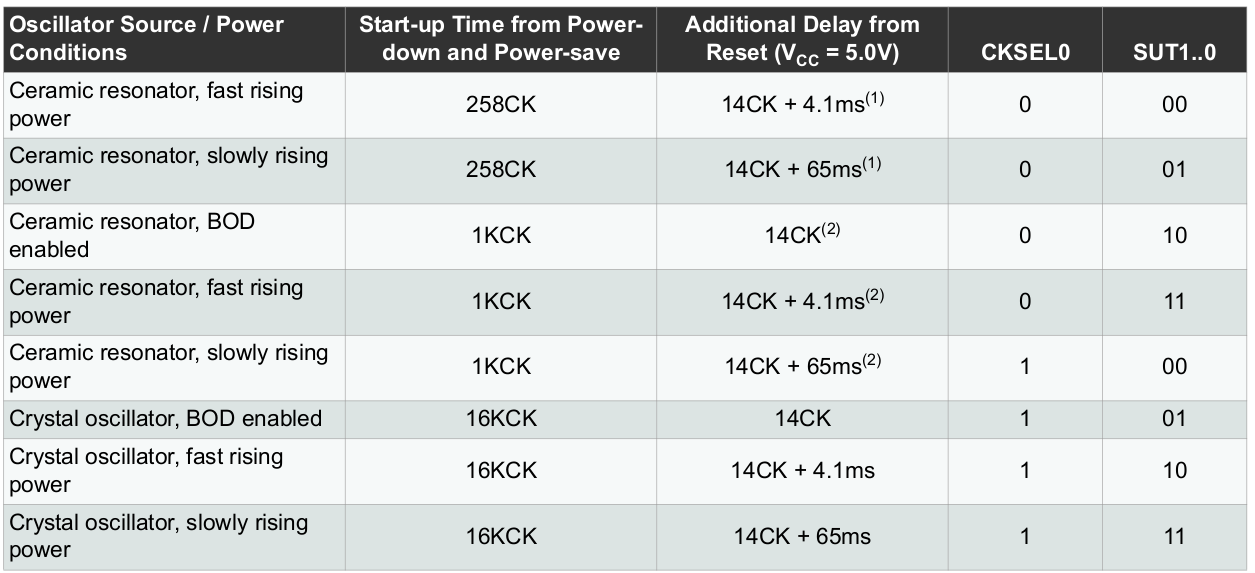
\includegraphics[width=0.95\textwidth]{startUpTimesLowPowerCrystallOscillator.png}
        \end{center}
    \end{figure}
\end{itemize}

\subsubsection{Full Swing Crystal Oscillator}

\begin{figure}[H]
	\begin{minipage}{.45\textwidth}
		\begin{center}
			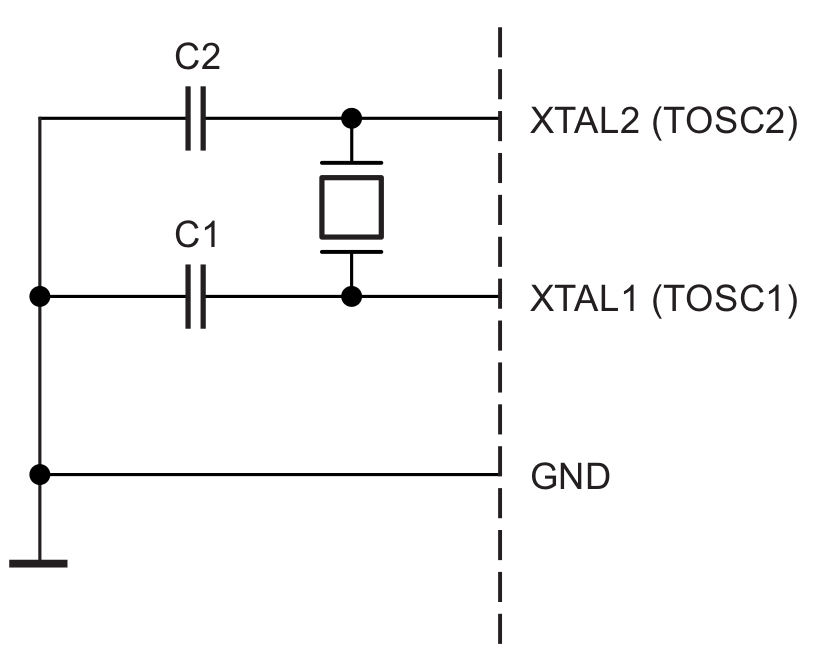
\includegraphics[width=0.45\textwidth]{fullSwingCrysallOscillatorCircuit.png}
			\caption{VGA Connector}
		\end{center}
	\end{minipage}
	\begin{minipage}{.5\textwidth}
		\begin{center}
            \begin{tabular}{c|c}
                \bitFormat{CKSEL[3:1]} & \textbf{Frequency Range (MHz)}\\
                \hline
                011 & 0.4 to 16.0\\
            \end{tabular}
		\end{center}
	\end{minipage}
\end{figure}


\begin{itemize}
    \item \pinFormat{XTAL1} and \pinFormat{XTAL2} are inputs and outpus of an inverting amplifier which can be configured as on-chip oscillator.
    \item Either Quartz Crystall or Ceramic resonator can be used.
    \item Full-Swing with rail-to-rail swing on the XTAL2 outtput.
    \item Can drive other clock input
    \item Power consumption is more than Low power crystal oscillator
    \item Needs $V_{CC}$ = 2.7 to 5.5V
    \item C1 and C2 should be of the same values – 12pF to 22pF.
    \item  The \bitFormat{CKSEL[0]} fuse together with the \bitFormat{SUT[1:0]} fuses select the start-up times as shown in Table below.
    \begin{figure}[H]
        \begin{center}
            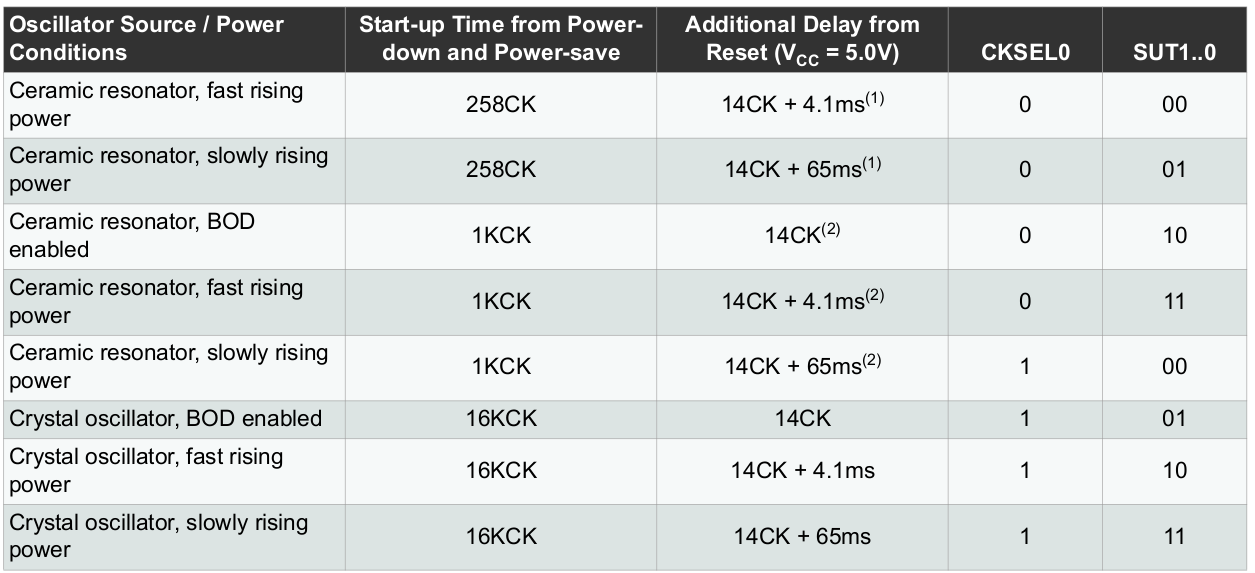
\includegraphics[width=0.95\textwidth]{startUpTimesLowPowerCrystallOscillator.png}
        \end{center}
    \end{figure}
\end{itemize}

\subsubsection{Low Frequency Crystal Oscillator}
\begin{itemize}
    \item To use with 32.765kHz watch crystal
    \item Crystal Cap(CL) – 6.5,9.0 and 12.5pF
    \item \bitFormat{CKSEL[3:0]} == 0101.
    \item The Start-up Times for the Low-frequency Crystal O scillator Clock Selection
    \begin{figure}[H]
        \begin{center}
            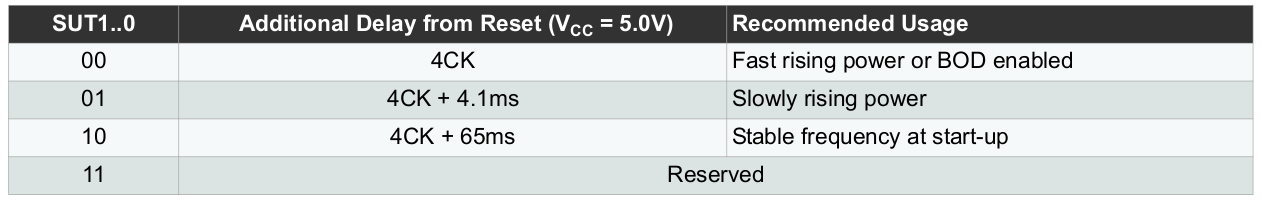
\includegraphics[width=0.95\textwidth]{startUpTimelowFrequencyCrysalOscillator.png}
        \end{center}
    \end{figure}
\end{itemize}

\subsubsection{Calibrated Internal RC Oscillator}
\begin{itemize}
    \item 8.0MHz clock
    \item Voltage and temperature dependent
    \item Calibration is done in \regFormat{OSCCAL}.
    \item Default mode shipeed with CKDIV8 prescalar programmed to prescale causing the system clock to be 1.0MHz.
    \item \bitFormat{CKSEL[3:0]} == 0010.
    \begin{figure}[H]
        \begin{center}
            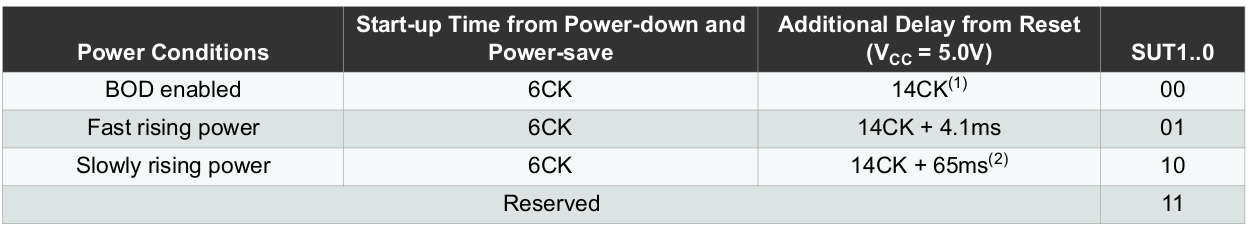
\includegraphics[width=0.95\textwidth]{startUpTimeCalibratedInternalRCOscillator.png}
        \end{center}
    \end{figure}
\end{itemize}

\subsubsection{128kHz Internal Oscillator}
\begin{itemize}
    \item low power oscillator with 128kHz frequency
    \item \bitFormat{CKSEL[3:0]} == 0010.
    \begin{figure}[H]
        \begin{center}
            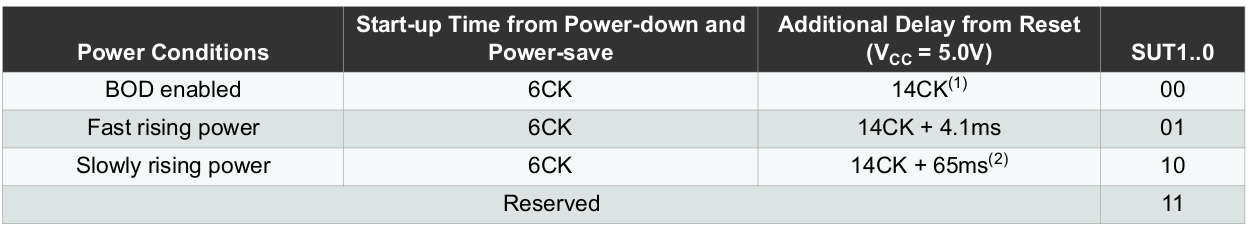
\includegraphics[width=0.95\textwidth]{startUpTimeCalibratedInternalRCOscillator.png}
        \end{center}
    \end{figure}
\end{itemize}

\subsubsection{External Clock}
\begin{figure}[H]
    \begin{center}
        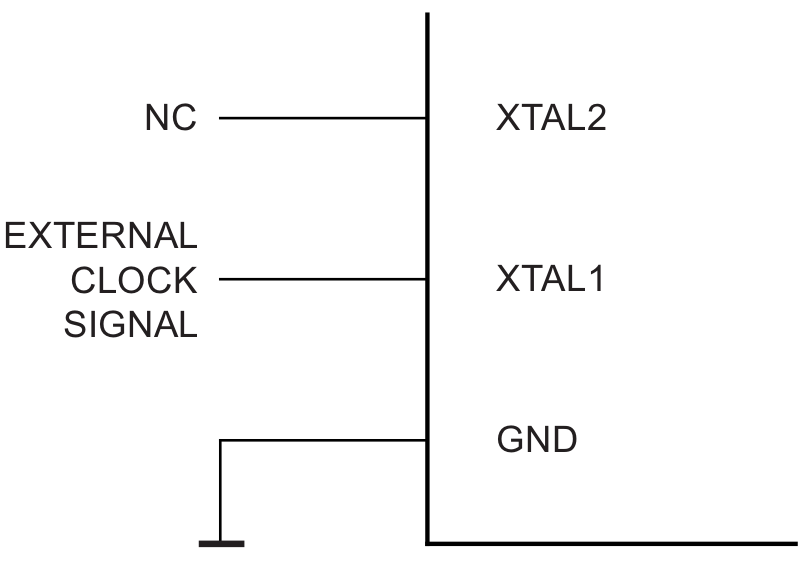
\includegraphics[width=0.25\textwidth]{externalClockciruit.png}
    \end{center}
\end{figure}
\begin{itemize}
    \item XTAL1 must be connected to external source.
    \item 0 - 16 MHz frequency.
    \item \bitFormat{CKSEL} == 0000.
    \item Start-up times are determined by the SUT fuses as
    \begin{figure}[H]
        \begin{center}
            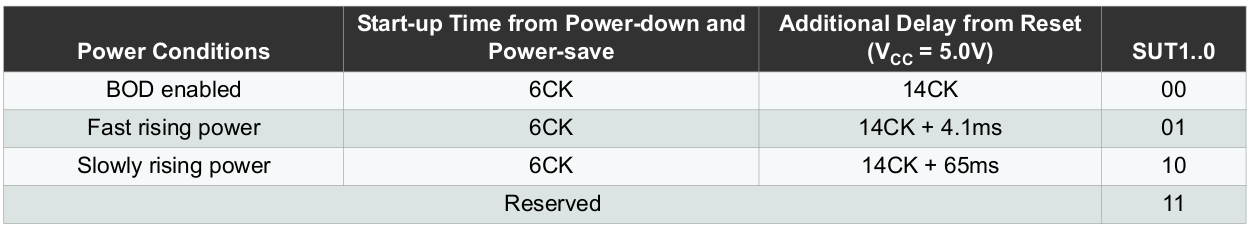
\includegraphics[width=0.95\textwidth]{startUpTimeExternalClock.png}
        \end{center}
    \end{figure}
\end{itemize}

\subsection{System Clock Prescalar}
\begin{itemize}
    \item The system clock can be divided by setting the \regFormat{CLKPR} (Clock Prescale Registers) value.
    \item Used to decrease the system clock frequency and the power consumption when the requirement for processing power is low.
    \item Affects the $clk_{SYS}$, $clk_{IO}$, $clk_{ADC}$, $clk_{CPU}$ and $clk_{FLASH}$.
    \item A special write procedure is followed to change \bitFormat{CLKPS} bits:
    \begin{enumerate}[label=(\roman*)]
        \item Write the clock prescaler change enable (\bitFormat{CLKPCE}) bit to one and all other bits in \regFormat{CLKPR} register to zero.
        \item Within four cycles, write the desired value to \bitFormat{CLKPS} bit while writing a zero to \bitFormat{CLKPCE}.
        \item Interrupt must be disabled.
    \end{enumerate}
\end{itemize}

\subsubsection{Register Description}
\subsubsection*{OSCCAL – Oscillator Calibration Register}
\vspace*{0.5cm}
\begin{bytefield}[bitformatting={\large\bfseries},
    endianness=big,bitwidth=0.125\linewidth]{8}
    \bitheader[lsb=0]{0-7} \\
    \bitbox{1}{\small CAL7}
    \bitbox{1}{\small CAL6}
    \bitbox{1}{\small CAL5}
    \bitbox{1}{\small CAL4}
    \bitbox{1}{\small CAL3}
    \bitbox{1}{\small CAL2}
    \bitbox{1}{\small CAL1}
    \bitbox{1}{\small CAL0}\\
\end{bytefield}
\begin{itemize}
    \item The oscillator calibration register is used to trim the calibrated internal RC oscillator to remove process variations from the oscillator frequency.
    \item A pre-programmed calibration value is automatically written to this register during chip reset.
    \item The application software can write this register to change the oscillator frequency.
    \item If EEPROM is to be used, shouldn't do calibration for more than 8.8 MHz.
    \item \bitFormat{CAL7} bit detected range of operation of oscillator. Setting zeros gives the Lowest requency range, setting this bit to 1 gives the highest frequency range.
    \item The \bitFormat{CAL[6:0]} bits are used to tune the frequency within the selected range. A setting of 0x00 gives the lowest frequency in that range, and a setting of 0x7F gives the highest frequency in the range.
\end{itemize}

\subsubsection*{CLKPR – Clock Prescale Register}
\vspace*{0.5cm}
\begin{bytefield}[bitformatting={\large\bfseries},
    endianness=big,bitwidth=0.125\linewidth]{8}
    \bitheader[lsb=0]{0-7} \\
    \bitbox{1}{\small CLKPCE}
    \bitbox{1}{\small -}
    \bitbox{1}{\small -}
    \bitbox{1}{\small -}
    \bitbox{1}{\small CLKPS3}
    \bitbox{1}{\small CLKPS2}
    \bitbox{1}{\small CLKPS1}
    \bitbox{1}{\small CLKPS0}\\
\end{bytefield}

\begin{itemize}
    \item \bitFormat{CLKPCE} - Cloc k Prescaler Change Enable must be written to logic one to enable change of the \bitFormat{CLKPS} bits.
    \item The \bitFormat{CLKPCE} bit is only updated when the other bits in CLKPR are simultaneously written to zero.
    
    \begin{table}[H]
        \begin{center}
            \begin{tabular}{c|c}
                \bitFormat{CLKPS[3:0]} & \textbf{Clock Division Facter}\\
                \hline
                0000 & 1\\
                0001 & 2\\
                0010 & 4\\
                0011 & 8\\
                0100 & 16\\
                0101 & 32\\
                0110 & 64\\
                0111 & 128\\
                1000 & 256\\                
            \end{tabular}
        \end{center}
    \end{table}

    \item \bitFormat{CLKPS[3:0]} - Clock Prescaler Select Bits define the division factor between the selected clock source and the internal system clock.
    \item The \bitFormat{CKDIV8} fuse determines the initial value of the \bitFormat{CLKPS} bits. 
    \begin{itemize}
        \item If \bitFormat{CKDIV8} is unprogrammed, the \bitFormat{CLKPS} bits will be reset to 0000.
        \item If \bitFormat{CKDIV8} is programmed, \bitFormat{CLKPS} bits are reset to “0011”, giving a division factor of 8 at start up.
    \end{itemize} 
    \item Note that any value can be written to the \bitFormat{CCLKPS} bits regardless of the \bitFormat{CCKDIV8} fuse setting.
\end{itemize}

\section{Power Management and Sleep modes}
\begin{itemize}
    \item Sleep modes enable the application to shut down unused modules in the MCU, thereby saving power.
    \item When enabled, the brown-out detector (BOD) actively monitors the power supply voltage during the sleep periods.
    \item To further save power, it is possible to disable the BOD in some sleep modes.
\end{itemize}

\subsection{Sleep Modes}
\begin{itemize}
    \item To enter any of the six sleep modes, the \bitFormat{SE} bit in \regFormat{SMCR} register must be written to logic one.
    \item The \bitFormat{SM[2:0]} bits in the \regFormat{SMCR} register select which sleep mode.
    \item \emph{SLEEP} instruction must be executed.
    \item If an enabled interrupt occurs while the MCU is in a sleep mode, the MCU wakes up.
    \item The MCU is then halted for four cycles in addition to the start-up time, executes the interrupt routine, and resumes execution from the instruction following SLEEP.
    \item The contents of the register file and SRAM are unaltered when the device wakes up from sleep. 
    \item If a reset occurs during sleep mode, the MCU wakes up and executes from the reset vector.
    \item The Active Clock Domains and Wake-up Sources in the Different Sleep Modes,
\end{itemize}
\begin{figure}[H]
    \begin{center}
        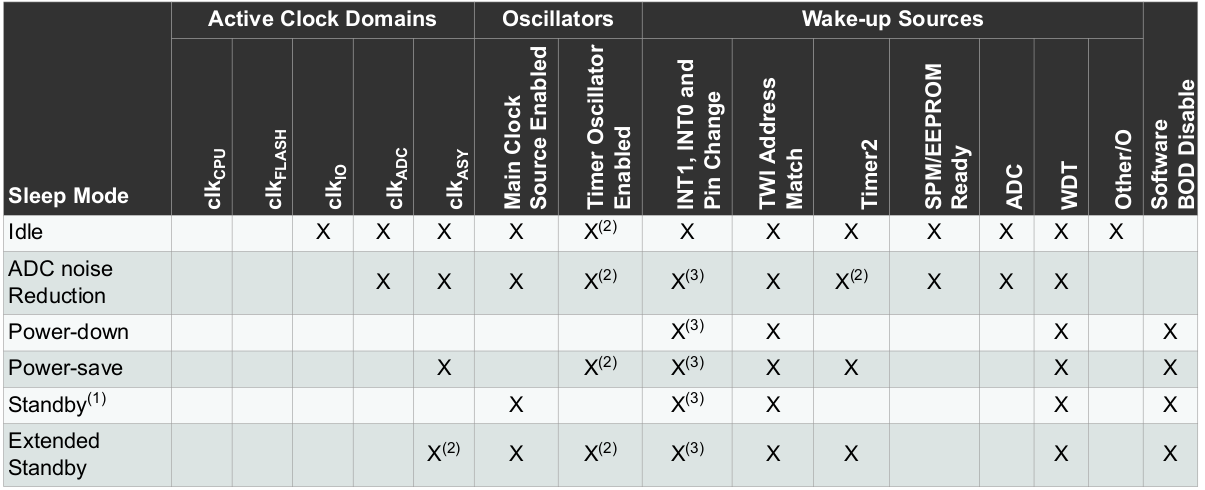
\includegraphics[width=1\textwidth]{sleepModeDomain.png}
    \end{center}
\end{figure}

\subsubsection{Idle Mode}
\begin{itemize}
    \item Stops the CPU but allows the SPI, USART, analog comparator, ADC, 2-wire serial interface, Timer/Counters, watchdog, and the interrupt
    system.
    \item Halts $clk_{CPU}$ and  $clk_{FLASH}$ and allows other clocks.
    \item Idle mode enables the MCU to wake up from external triggered interrupts as well as internal ones like the timer overflow and USART transmit complete interrupts.
\end{itemize}

\subsubsection{ADC Noise Reduction Mode}
\begin{itemize}
    \item Stops the CPU but allows ADC, the external interrupts, the 2-wire serial interface address watch, Timer/Counter2 and the watchdog.
    \item Halts $clk_{I/O}$, $clk_{CPU}$ and  $clk_{FLASH}$ and allows other clocks.
    \item Improves the noise environment for ADC, enabling higher resolution measurement.
    \item ADC Noise Reduction Mode enables the MCU to wake up from external reset, a watchdog system reset, a watchdog interrupt, a brown-out reset, a 2-wire serial interface address match, a Timer/Counter2 interrupt, an SPM/EEPROM ready interrupt, an external level interrupt on INT0 or INT1 or a pin change interrupt.
\end{itemize}

\subsubsection{Power-down Mode}
\begin{itemize}
    \item Stops the external oscillator but allows the external interrupts, the 2-wire serial interface address watch, and the watchdog.
    \item Halts all clocks and asynchronous modules only.
    \item Power-down mode enables the MCU to wake up from an external reset, a watchdog system reset, a watchdog interrupt, a brown-out reset, a 2-wire serial interface address match, an external level interrupt on INT0 or INT1, or a pin change interrupt.
\end{itemize}


\subsubsection{Power-save Mode}
\begin{itemize}
    \item Only diffence from Power-down mode is Timer/Counter2 is enabled and it will run.
    \item Timer overflow or output compare event from Timer/Counter2 can wake up.
\end{itemize}

\subsubsection{Standby Mode}
\begin{itemize}
    \item Selects the external crystal clock option.
    \item Identical to power-down except oscillator is running.
\end{itemize}

\subsubsection{External Standby Mode}
\begin{itemize}
    \item Selects the external crystal clock option.
    \item Identical to power-Save except oscillator is running.
\end{itemize}

\subsubsection{Register Description}
\subsubsection*{SMCR – Sleep Mode Control Register}
\vspace*{0.5cm}
\begin{bytefield}[bitformatting={\large\bfseries},
    endianness=big,bitwidth=0.125\linewidth]{8}
    \bitheader[lsb=0]{0-7} \\
    \bitbox{1}{\small -}
    \bitbox{1}{\small -}
    \bitbox{1}{\small -}
    \bitbox{1}{\small -}
    \bitbox{1}{\small SM2}
    \bitbox{1}{\small SM1}
    \bitbox{1}{\small SM0}
    \bitbox{1}{\small SE}\\
\end{bytefield}

\begin{table}[H]
    \begin{center}
        \begin{tabular}{c|c}
            \bitFormat{SM[2:0]} & \textbf{Sleep Mode}\\
            \hline
            000 & Idle\\
            001 & ADC Noise Reduction\\
            010 & Power-down\\
            011 & Power-save\\
            110 & Standby\\
            111 & External Standby\\
        \end{tabular}
    \end{center}
\end{table}
\begin{itemize}
    \item \bitFormat{SE} bit must be written to logic one  just before the SLEEP instruction is executed, to make the MCU enter the sleep mode.
\end{itemize}

\subsection{Power Reduction Register}
\begin{itemize}
    \item To stop the clock to individual peripherals to reduce power consumption.
    \item The current state of the peripheral is frozen and the I/O registers can not be read or written.
    \item Peripheral should in most cases be disabled before stopping the clock.
    \item Wake up peripherals can be done by writing zero to bits in \regFormat{PRR}.
\end{itemize}

\subsubsection{Register Description}
\subsubsection*{PRR – Power Reduction Register}
\vspace*{0.5cm}
\begin{bytefield}[bitformatting={\large\bfseries},
    endianness=big,bitwidth=0.125\linewidth]{8}
    \bitheader[lsb=0]{0-7} \\
    \bitbox{1}{\small PRTWI}
    \bitbox{1}{\small PRTIM2}
    \bitbox{1}{\small PRTIM0}
    \bitbox{1}{\small -}
    \bitbox{1}{\small PRTIM1}
    \bitbox{1}{\small PRSPI}
    \bitbox{1}{\small PRUSART0}
    \bitbox{1}{\small PRADC}\\
\end{bytefield}


\begin{table}[H]
    \begin{center}
        \begin{tabular}{c|c}
            \textbf{Bits} & \textbf{Name}\\
            \hline
            \bitFormat{PRTWI} & Power Reduction TWI\\
            \bitFormat{PRTIM2} & Power Reduction Timer/Counter2\\
            \bitFormat{PRTIM1} & Power Reduction Timer/Counter1\\
            \bitFormat{PRTIM0} & Power Reduction Timer/Counter0\\
            \bitFormat{PRSPI} & Power Reduction Serial Peripheral Interface\\
            \bitFormat{PRUSART0} & Power Reduction USART0\\
            \bitFormat{PRADC} & Power Reduction ADC\\
        \end{tabular}
    \end{center}
\end{table}

\subsection{Minimizing Power Consumption}
\begin{itemize}
    \item In general, sleep modes should be used as much as possible.
    \item ADC should be disabled before entering any sleep mode.
    \item Analog comparator should be disabled in  all sleep modes.
    \item If the brown-out detector is not needed by the application, this module should be turned off by \bitFormat{BODLEVEL} fuses.
    \item If Internal Voltage Reference is not needded and ADC or analog comparator or BOD is not needed, the Internal Voltage Reference can be disabled.
    \item If the watchdog timer is not needed in the application, the module should be turned off.
    \item If On-chip Debug System is not needed, can be disabled by \bitFormat{DWEN} fuse.
    \item For Port pins,
    \begin{itemize}
        \item No pins drive resistive loads.
        \item Input buffers are disabled when I/O clock and ADC clocks are stopped.
        \item If the input buffer is enabled and the input signal is left floating or have an analog signal level close to V CC /2, the input buffer will use excessive power.
        \item Digital input buffers can be disabled by writing to the digital input disable registers (\regFormat{DIDR1} and \regFormat{DIDR0}).
    \end{itemize}
\end{itemize}

\section{RESETTING AVR}
\quad All I/O registers are set to their intial values and program starts execution form reset vector.

\begin{figure}[H]
    \begin{center}
        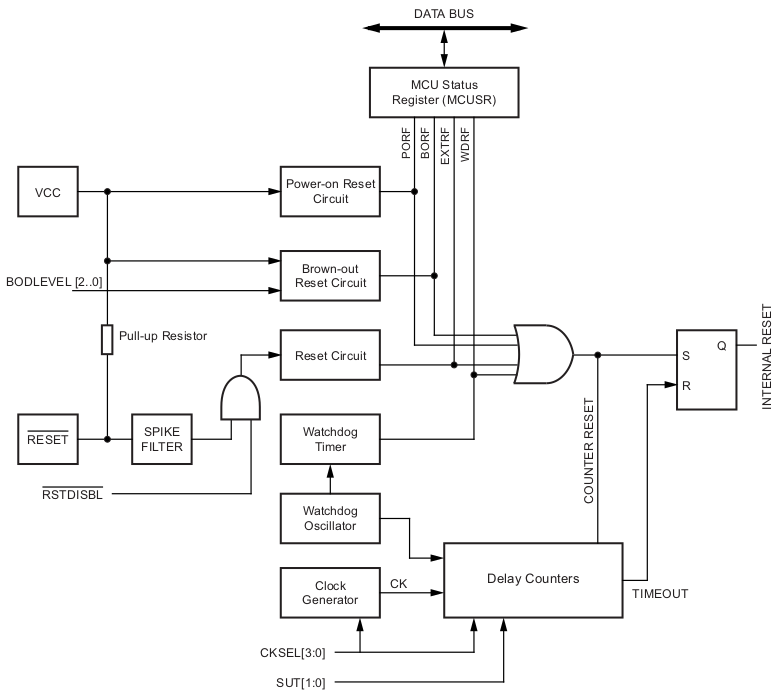
\includegraphics[height=0.55\textheight]{resetLogic.png}
    \end{center}
\end{figure}

\subsection{Reset Sources}
\begin{enumerate}[label=(\Roman*)]
    \item Power-on Reset - MCU resets when supply voltage is below the power-on reset threshold($V_{POT}$).
    \item External Reset - MCU resets when low level is present on \pinFormat{$\overline{RESET}$} is helow for minimum pulse length.
    \item Watchdog System reset - MCU resets when watchdog timer period expires and watchdog system reset mode is enabled.
    \item Brown-out reset - MCU resets when supply voltage $V_{CC}$ is below brown-out threshold ($V_{BOT}$) and brown-out detected is enabled.
\end{enumerate}

\subsubsection{Power-on Reset}
\begin{figure}[H]
    \begin{minipage}{0.45\textwidth}
        \begin{center}
            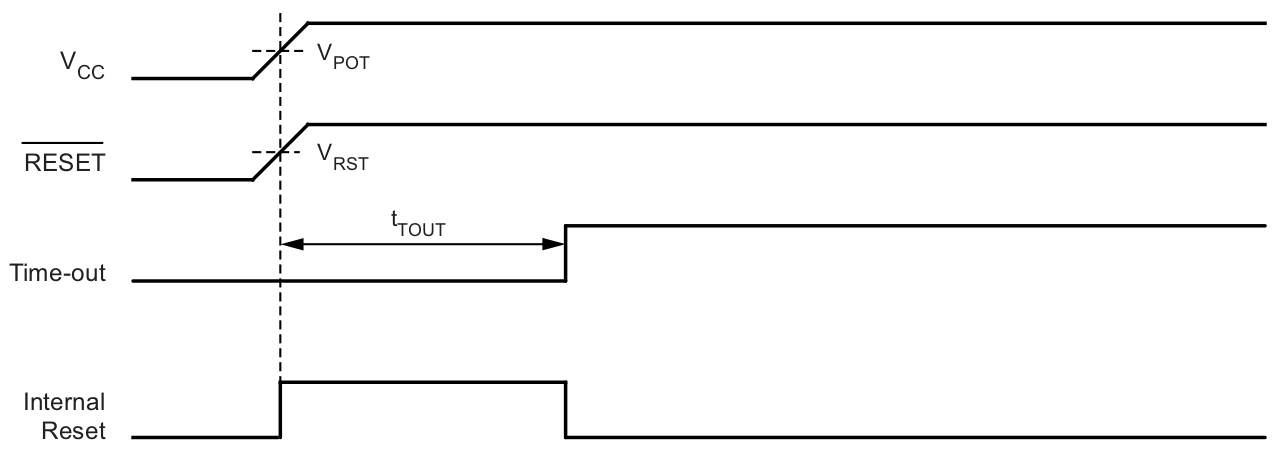
\includegraphics[width=1\textwidth]{POR1.png}
            \caption*{MCU Start-up, $\overline{RESET}$ Tied to $V_{CC}$}
        \end{center}
    \end{minipage}
    \begin{minipage}{0.5\textwidth}
        \begin{center}
            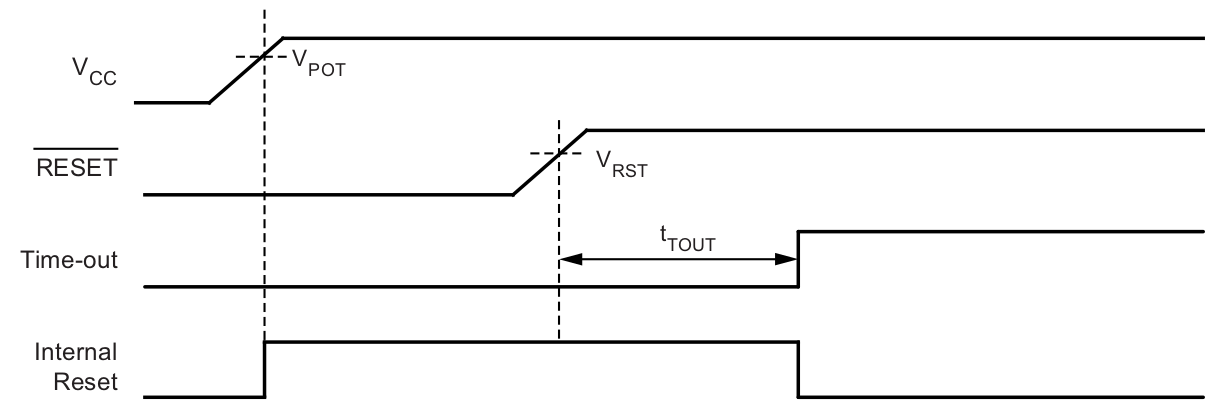
\includegraphics[width=1\textwidth]{POR2.png}
            \caption*{MCU Start-up, $\overline{RESET}$ Extended Externally}
        \end{center}
    \end{minipage}
\end{figure}
\begin{itemize}
    \item A power-on reset (POR) pulse is generated by an on-chip detection circuit.
    \item The POR is activated whenever $V_{CC}$ is below the detection level.
    \item The POR circuit can be used to trigger the start-up reset, as well as to detect a failure in supply voltage.
    \item Reaching the power-on reset threshold voltage invokes the delay counter, which determines how long the device is kept in RESET after $V_{CC}$ rise.
\end{itemize}


\subsubsection{External Reset}
\begin{figure}[H]
    \begin{center}
        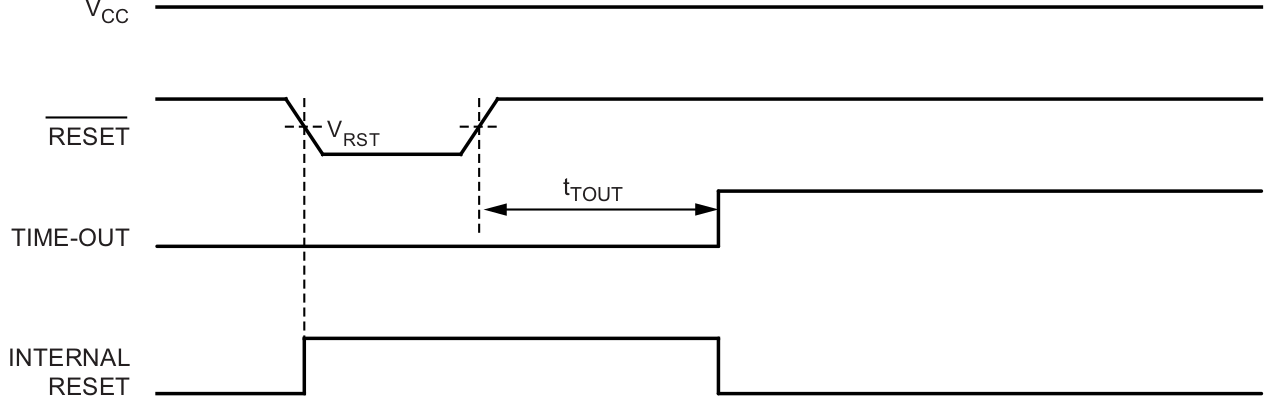
\includegraphics[width=0.5\textwidth]{externalReset.png}
    \end{center}
\end{figure}
\begin{itemize}
    \item An external reset is generated by a low level on the \pinFormat{$\overline{RESET}$}  pin.
    \item Shorter pulses are not guaranteed to generate a reset.
    \item When the applied signal reaches the reset threshold voltage – $V_{RST}$ – on its positive edge, the delay counter starts the MCU after the time-out period – $t_{OUT}$ – has expired.
    \item The external reset can be disabled by the \bitFormat{RSTDISBL} fuse.
\end{itemize}

\subsubsection{Brown-out Detection}
\begin{figure}[H]
    \begin{center}
        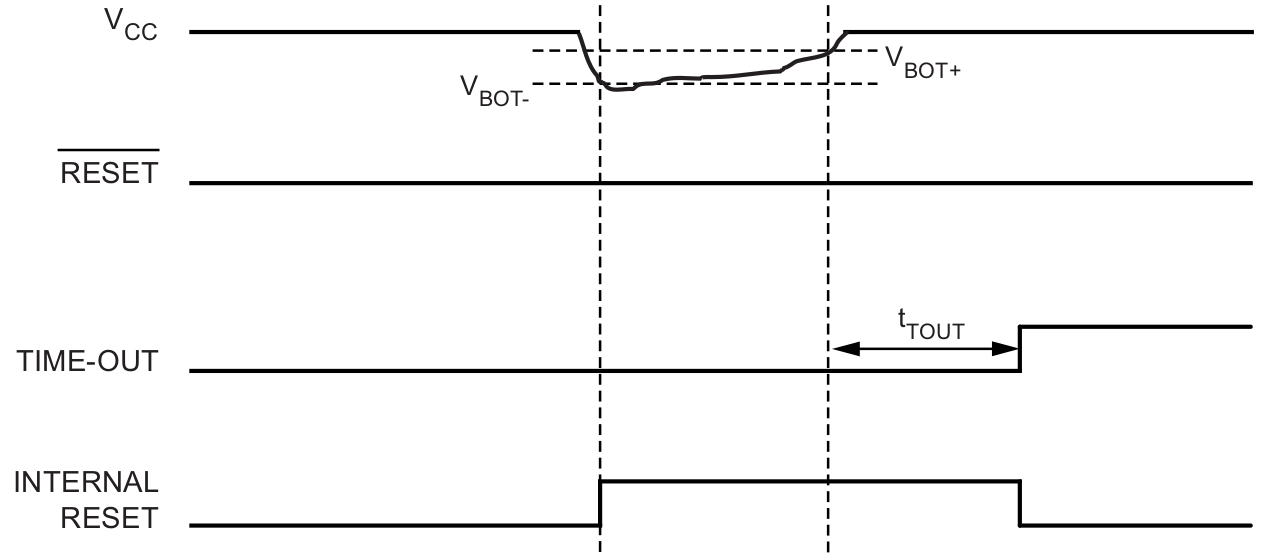
\includegraphics[width=0.5\textwidth]{brownOutReset.png}
    \end{center}
\end{figure}
\begin{itemize}
    \item On-chip brown-out detection (BOD) circuit for monitoring the $V_{CC}$ level during operation by comparing it to a fixed trigger level.
    \item The trigger level for the BOD can be selected by the \bitFormat{BODLEVEL} fuses.
\end{itemize}

\subsubsection{Watchdog System Reset}
\begin{figure}[H]
    \begin{center}
        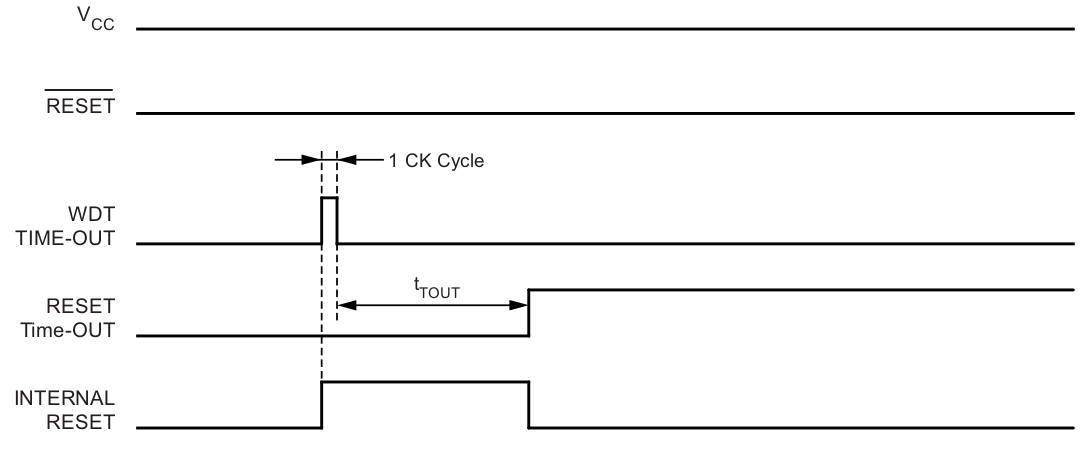
\includegraphics[width=0.5\textwidth]{watchDogReset.png}
    \end{center}
\end{figure}
\begin{itemize}
    \item When the watchdog times out, it will generate a short reset pulse of one CK cycle duration.
    \item On the falling edge of this pulse,
    the delay timer starts counting the time-out period $t_{OUT}$.
\end{itemize}


% \end{document}


\chapter{Compiling and Running}
\documentclass{article}

\usepackage[a4paper, left=0.5in, right=0.5in, bottom=0.5in, top=0.5in]{geometry}
\usepackage{hyperref} 
\hypersetup{
    colorlinks=true,      
    urlcolor=blue
}

\usepackage{enumitem}
\usepackage{xcolor}
\usepackage{natbib}

\usepackage{minted}

\usepackage{ragged2e}
\begin{document}
\justify

\subsection*{GCC\cite{toolChain}}
\begin{itemize}
    \item GNU Compiler Collectin - compiler system.
    \item Supports various language, processor and host operating system.
    \item AVR GCC - Reffering to GCC targeting AVR.
    \item AVR GCC translates high-level langues to assembly.
    \item AVR GCC three language - C, C++, Ada.
\end{itemize}

\subsection*{GNU Binutils\cite{toolChain}} 
Source : \href{https://www.nongnu.org/avr-libc/user-manual/overview.html}{Tool Chain overview}
\begin{itemize}
    \item Binary Utilites - contains the GNU assembler(gas), GNU linker(ld), etc.
    \item avr-as - The assembler.
    \item avr-ld - The linker.
    \item avr-objcopy - Copy and translate object files to different format.
    \item avr-objdump - Display information from object file including disassembly.
    \item avr-size - List section sizes and total sizes.
    \item avr-nm - List symbols from objects files.
    \item avr-strings - List printable strings from files.
    \item avr-readelf - Display contents of ELF files.
    \item avr-addr2line - Convert addresses to file and line.
\end{itemize}

\subsection*{avr-lib\cite{toolChain}}
\quad Open source standard C Libary - standard C Libary and Libary function specifit to AVR.



\subsection*{Compiler Options\cite{compilerOptimize}} \label{optimization}
\emph{-On} -- for optimization level; n indicates the optimization level; 0 being the default no optimization; 
\begin{itemize}
    \item \emph{-O0} -- reduces compilation time and this is default
    \item \emph{-O} and \emph{-O1} -- the compiler tries to reduce code size and execution time, without performing any optimizations that take a great deal of compilation time.
    \item \emph{-O2} --  Optimize even more than \emph{-O1}
    \item \emph{-O3} --  Optimize even more than \emph{-O2}
    \item \emph{-Os} -- Optimize for size and enables all \emph{-O2} optimization but not expected to increase code size
    \item \emph{-Ofast} -- enables all \emph{-O3} optimzations and disregarads strict standard compliance
    \item \emph{-Og} -- Optimize for debugging experience
\end{itemize}


\subsection*{Compilation} 
\begin{itemize}
    \item Will create the .obj object binary files.
    \item Use \emph{avr-gcc} along with following options
    \begin{itemize}
        \item Optimization option \emph{-On} - use \emph{-Os} generally.
        \item Warning option \emph{-Wall} - enables all the warning
        \item Debug option \emph{-g} - Produce debugging information.
        \item MCU option \emph{-mmcu} - the actual MCU - \href{https://www.nongnu.org/avr-libc/user-manual/#supp_devices}{Supported MCU}
        \item C file option \emph{-c} - the actual c file.
        \item Output file name \emph{-o} - Output file name
    \end{itemize}
    \item To see the object binary file use \emph{avr-objdump -S fileName.o}
    \mint[bgcolor=lightgray]{shell}{avr-gcc -Os -Wall -g -mmcu=atmega8 -c hello.c -o hello.o}
\end{itemize}


\subsection*{Linking}
\begin{itemize}
    \item Link the bianary object file to binary elf file.
    \item Use \emph{avr-gcc} along with following options
    \begin{itemize}
        \item Optimization option \emph{-On} - use \emph{-Os} generally.
        \item Warning option \emph{-Wall} - enables all the warning
        \item Debug option \emph{-g} - Produce debugging information.
        \item MCU option \emph{-mmcu} - the actual MCU - \href{https://www.nongnu.org/avr-libc/user-manual/#supp_devices}{Supported MCU}
        \item .obj file option - the actual .obj file.
        \item Output file name \emph{-o} - Output file name

    \end{itemize}
    \item To see the object binary file use \emph{avr-objdump -S fileName.elf}
    \mint[bgcolor=lightgray]{shell}{avr-gcc -Os -Wall -g -mmcu=atmega8 hello.o -o hello.elf}
\end{itemize}

\subsection*{Generating the hex file}
\begin{itemize}
    \item The Intel hex file is what we program into procesosr.
    \item Use \emph{avr-objcopy} along with following options
    \begin{itemize}
        \item section Option \emph{-j} -- which sections to copy - generally .text and .data section
        \item Output format option \emph{-O} - what Output format should be used - eg) ihex
        \item The input .elf file
        \item The output .hex file
    \end{itemize}
    \mint[bgcolor=lightgray]{shell}{avr-objcopy -j .text -j .data -O ihex hello.elf hello.hex}

\end{itemize}

\section*{AVRDUDE\cite{avrdude}}
\subsection*{Introduction}
\begin{itemize}
    \item AVRDUDE - AVR Downloader UploDEr is a program for downloading and uploading the on-chip memories of Atmel's AVR microcontroller.
    \item Can program Flash, EEPROM, fuse ,lock bits and  signature bytes.
    \item Can read or write all chip memory types mentioned above.
    \item Supports varieous programmers from STK500, AVRISP, mkII, JTAG ICE, PPI, serial bit-bang adapters, etc.
    \item The STK500, JTAG ICE, etc uses serial port to communicate.
    \item The JTAGICE, AVRISP, USBasp, USBtinyISP uses USB using \emph{libusb}.
\end{itemize}


\subsection*{Command Line Options}
\begin{itemize}
    \item \emph{-p partno} -- the mandatory option which specifies the MCU.
    \item \emph{-b baudrate} -- Specify the Baudrate.
    \item \emph{-c programmer-id} -- Specify the pgorammer used. eg)arduino, avrisp, avrisp2, avrispmkII, avrispv2, jtag1, stk500, stk500v1, stk500v2, usbasp, usbtiny, etc.
    \item \emph{-C config-file} -- Configuration data file.
    \item \emph{-e} -- Causes a chip erase of FLash ROM, EEPROM to 0xff and clears all lock bits.
    \item \emph{-F} -- Override device signature check.
    \item \emph{-P port} -- Specifty the port to be used.
    \item \emph{-u} -- Used if you want to write fuse bits - this cuases disabling the safemode for fuse bits.
    \item \emph{-t} -- uses interactive terminal mode instead of up or downloading files.
    \item \emph{-v} -- Verbose
    \item \emph{-U memtype:op:filename[:format]}
    \begin{itemize}
        \item \emph{memtype} -- Memory types are 
        \begin{enumerate}[label=(\roman*)]
            \item \emph{calibration} -- One or more bytes of RC oscillator calibration data.
            \item \emph{eeprom} -- The EEPROM.
            \item \emph{efuse} -- The extended fuse byte
            \item \emph{flash} -- The flash ROM of device
            \item \emph{fuse} -- The fuse byte in devices with a single fuse byte.
            \item \emph{hfuse} -- The high fuse byte.
            \item \emph{lfuse} -- The low fuse byte.
            \item \emph{lock} - The lock byte.
            \item \emph{signature} - The three device signature byte (device ID).
        \end{enumerate}
        \item \emph{op} -- Operations are
        \begin{enumerate}[label=(\roman*)]
            \item \emph{r} -- Read the specifed device memory and write to specified file.
            \item \emph{w} -- read the specifed file and write to specifed device memory.
            \item \emph{v} -- read the specified device memory and the specified file and perform a verify operation .
        \end{enumerate}
        \item The \emph{filename} can be either a fileName,  immediate byte value (in decimal, binary,hexadecimal, etc)
        \item \emph{format} is optional and can 
        \begin{enumerate}
            \item \emph{i} - Intel hex
            \item \emph{r} - raw binary
            \item \emph{e} - the elf files
            \item \emph{m} - immediate mode
            \item \emph{d} - decimal
            \item \emph{b} - binary(0b)
            \item \emph{d} - hexadecimal(0x)
        \end{enumerate}
    \end{itemize}
\end{itemize}


\subsection*{Example}

\subsubsection*{Downloading hex file into device Flash}
\begin{minted}[bgcolor=lightgray]{bash}
    avrdude -p atmega8 -b 19200 -c stk500 -p /dev/ttyUSB0 -v -U flash:w:hello.hex:i
\end{minted}

\subsubsection*{Uploading Flash from device into file}
\begin{minted}[bgcolor=lightgray]{bash}
    avrdude -p atmega8 -b 19200 -c stk500 -p /dev/ttyUSB0 -v -U flash:r:"./readFashMemory.bin":r
\end{minted}

\subsubsection*{Reading Device signature}
\begin{minted}[bgcolor=lightgray]{bash}
    avrdude -p atmega8 -b 19200 -c stk500 -p /dev/ttyUSB0 -v -U signature:r:"deviceSinature.text":h
\end{minted}


\subsubsection*{Writing the High fuse}
\begin{minted}[bgcolor=lightgray]{bash}
    avrdude -p atmega8 -b 19200 -c stk500 -p /dev/ttyUSB0 -v -U hfuse:w:0x65:m
\end{minted}

Also see this\cite{alsosee}.

\bibliographystyle{plain}
\bibliography{ReferenceM}

\end{document}

\chapter{Input/Output Ports}
\documentclass{article}

\usepackage{NeededPackages}



\begin{document}


\section{Introduction}
\begin{itemize}
    \item The directin/drive value/pull-up register of one port pin can be changed without changing the directin/drive value/pull-up register  of any other pin - true \emph{read-modify-write}.
    \item Each output buffer has symmetrical drive characteristics with both high sink and source capability.
    \item All I/Opins have protection diode to both $V_{CC}$ and Ground.
    \begin{figure}[H]
        \begin{center}
            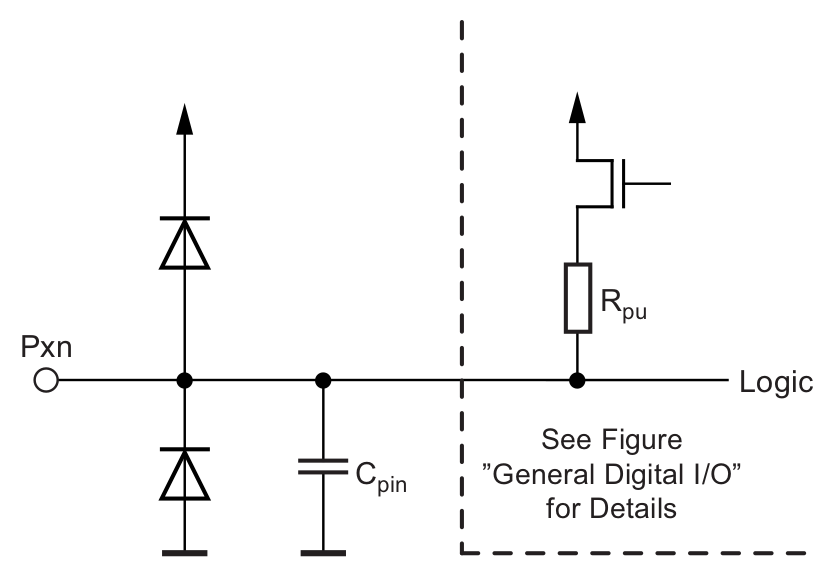
\includegraphics[width=0.5\textwidth]{IOpinEquivalent.png}
        \end{center}
    \end{figure}
    \item Three I/O memory address locations are allocated for each port, one each for the data register – \regFormat{PORTx}, data direction register – \regFormat{DDRx}, and the port input pins – \regFormat{PINx}.
    \item Most pins are multiplexed with alternative functions.
    \item Generally, after reset, the port pins are tri-stated.
    \item Disbaling the \bitFormat{PUD} bit in \regFormat{MCUCR} register disables the pull-up function of all pins.
    \item Unconnected pins should not float and must be connected to internal pull-up or external pull-up/pull-down registor.
\end{itemize}


\section{General Digital I/O}
\begin{figure}[H]
    \begin{center}
        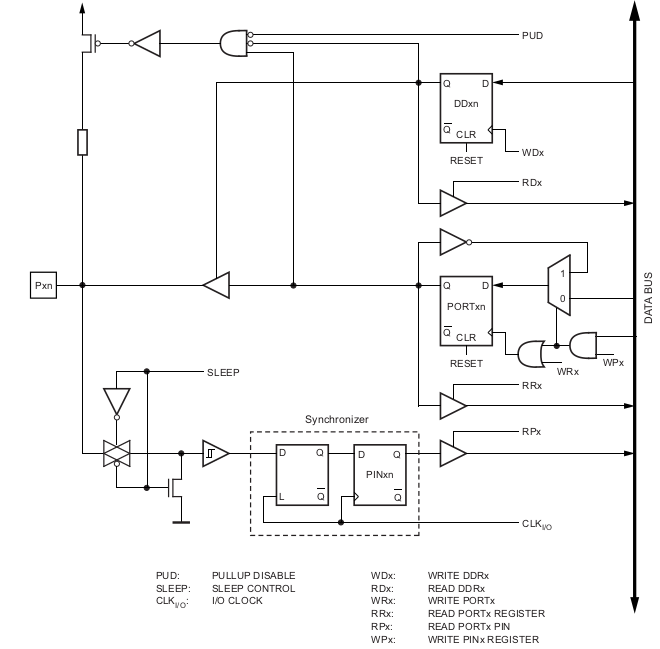
\includegraphics[width=1\textwidth]{IOcomplete.png}
    \end{center}
\end{figure}

\subsection{DDR Registers}
\begin{itemize}
    \item It is used to select the direction of a pin.
    \item DDxn == 1 $-->$ Pin n of Port x is configured as output.
    \item DDxn == 0 $-->$ Pin n of Port x is configured as input.
\end{itemize}

\subsection{PORT registers}
\begin{itemize}
    \item If the pin is configured as Output - Drive the pin.
    \begin{itemize}
        \item PORTxn == 1 $-->$ Pin n of Port x is driven to logic HIGH.
        \item PORTxn == 0 $-->$ Pin n of Port x is driven to logic LOW.
    \end{itemize}
    \item If the pin is configured as Input - configure pull-up resistor.
    \begin{itemize}
        \item PORTxn == 1 $-->$ Pin n of Port x has pull-up resistor activaed.
        \item PORTxn == 0 $-->$ Pin n of Port x has pull-up resistor deactivaed.
    \end{itemize}
\end{itemize}

\subsection{PIN Registers}
\begin{itemize}
    \item It is used to read the status of a pin.
    \item Writing 1 to a PINxn makes the Pin n of Port x toggle.
\end{itemize}

\section{Alternate Port Functions}
\begin{figure}[H]
    \begin{center}
        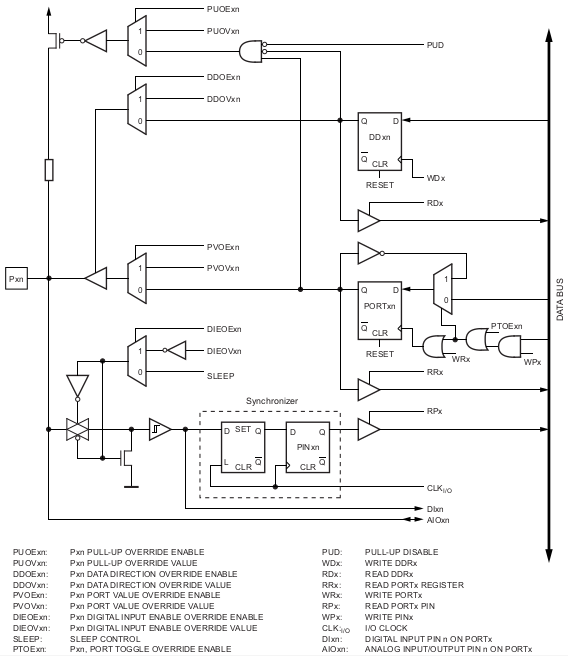
\includegraphics[width=1\textwidth]{IOalternatefunc.png}
    \end{center}
\end{figure}

\begin{figure}[H]
    \begin{center}
        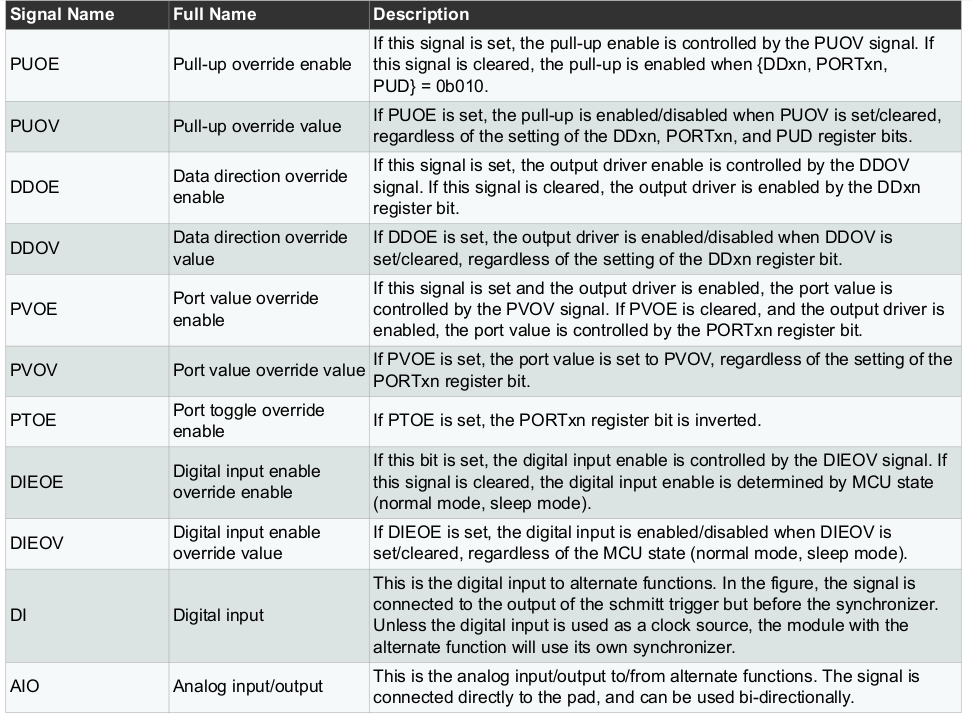
\includegraphics[width=1\textwidth]{IOsignals.png}
    \end{center}
\end{figure}


\end{document}



\chapter{Interrupts}
\documentclass{article}

\usepackage[a4paper, bottom=0.5in, top=0.5in, left=0.5in, right=0.5in]{geometry}
\usepackage{wrapfig}
\usepackage{natbib}
\usepackage{url}
\usepackage{xcolor}
\usepackage{caption}
\usepackage{hyperref}
\hypersetup{
    colorlinks=true,    
    urlcolor=cyan,
}
\usepackage{bytefield}

\usepackage{amsfonts}
\usepackage{float}
\usepackage{enumitem}

\usepackage{minted}

\newcommand{\bitFormat}[1]{\emph{\textbf{\textcolor{cyan}{#1}}}}

\newcommand{\regFormat}[1]{\textbf{\textcolor{magenta}{#1}}}

\newcommand{\pinFormat}[1]{\emph{\textcolor{red}{#1}}}


\usepackage{graphicx}
\graphicspath{ {./Resources/pics/} }



\title{ATmega328P Interrupts}
\author{Narendiran S}
\date{\today}

\begin{document}
\maketitle

\section{Introduction}
\begin{itemize}
    \item Each interrupt vector occupies two instruction Word(2x16bit) in Atmega328p.
    \item The complete placement of Reset and Interrupt Vectors in ATmega328P
    \begin{figure}[H]
        \begin{center}
            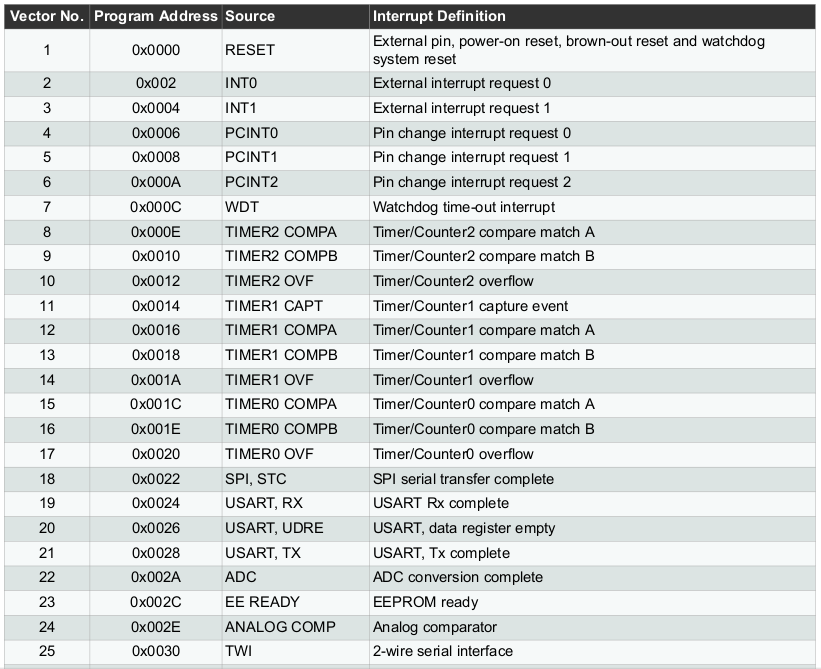
\includegraphics[height=.4\textheight]{resetAndInterruptVectors.png}
        \end{center}
    \end{figure}
    \item The location of reset vector is affected by \bitFormat{BOOTRST} fuse.
    \item The Interrupt vector start address is affected by \bitFormat{IVSEL} bit in \regFormat{MCUCR} register.
    \item The reset and interrupt Vector placement is shown below as
\end{itemize}
\begin{table}[H]
    \begin{minipage}{0.45\textwidth}
        \begin{center}
            \begin{tabular}{c|c}
                \bitFormat{BOOTRST} & \textbf{Reset Address}\\
                \hline
                0 & Boot reset address\\
                1 & 0x0000
            \end{tabular}
        \end{center}
    \end{minipage}
    \begin{minipage}{0.5\textwidth}
        \begin{center}
            \begin{tabular}{c|c}
                \bitFormat{IVSEL} & \textbf{Interrupt Vectors Start Address}\\
                \hline
                0 & 0x0002\\
                1 & Boot reset address + 0x0002
            \end{tabular}
        \end{center}
    \end{minipage}
\end{table}

\subsection{Register Description}
\subsubsection*{MCUCR – MCU Control Register}
\vspace*{0.5cm}
\begin{bytefield}[bitformatting={\large\bfseries},
    endianness=big,bitwidth=0.125\linewidth]{8}
    \bitheader[lsb=0]{0-7} \\
    \bitbox{1}{\small -}
    \bitbox{1}{\small BODS}
    \bitbox{1}{\small BODSE}
    \bitbox{1}{\small PUD}
    \bitbox{1}{\small -}
    \bitbox{1}{\small -}
    \bitbox{1}{\small IVSEL}
    \bitbox{1}{\small IVCE}\\
\end{bytefield}

\begin{itemize}
    \item When \bitFormat{IVSEL} bit is cleared, the interrupt vectors are placed at the start of the flash memory - the application section.
        \begin{itemize}
            \item When the \bitFormat{BLB12} is programmed, interrupts are disabled while executing from boot loader section.
        \end{itemize}
    \item When \bitFormat{IVSEL} bit is set, the interrupt vectors are moved to the beginning of the boot loader section of the flash. 
        \begin{itemize}
            \item When the \bitFormat{BLB02} is programmed, interrupts are disabled while executing from application section.
        \end{itemize}
    \item The actual address of the start of the boot flash section is determined by the \bitFormat{BOOTSZ} fuses.
    \item Writing \bitFormat{IVSEL} bit is done by
    \begin{enumerate}[label=(\alph*)]
        \item Write interrupt vector change enable \bitFormat{IVCE} bit to one.
        \item Write desired value to \bitFormat{IVSEL} while Writing zeros to \bitFormat{IVCE}.
    \end{enumerate}
    \item \bitFormat{IVCE} is cleared by hardware.
\end{itemize}

\section{External Interrupts}
\begin{itemize}
    \item Triggered by \pinFormat{INT0}, \pinFormat{INT1} and \pinFormat{PCING[23:0]} pins.
    \item Pin changed interrupt \emph{PCI2} will be triggered if any \pinFormat{PCINT[23:16]} toggles based on the \regFormat{PCMSK2} register.
    \item Pin changed interrupt \emph{PCI1} will be triggered if any \pinFormat{PCINT[14:8]} toggles based on the \regFormat{PCMSK1} register.
    \item Pin changed interrupt \emph{PCI0} will be triggered if any \pinFormat{PCINT[7:0]} toggles based on the \regFormat{PCMSK0} register.
    \item Due to asynchronous nature of Pin change interrupts, \pinFormat{PCINT[23:0]} can be used to wake up.
    \item The \pinFormat{INT0} and \pinFormat{INT1} can be triggered by falling, rising or low level choosen by \regFormat{EICRA} - External Interrupt Control Register.
    \item Due to asynchronous nature of External interrupts in low level interrupt, \pinFormat{INT0} and \pinFormat{INT1}  can be used to wake up.
 \end{itemize}

 \subsection{Register Description}
 \subsubsection*{EICRA - External Interrupt Control Register A}
 \vspace*{0.5cm}
\begin{bytefield}[bitformatting={\large\bfseries},
    endianness=big,bitwidth=0.125\linewidth]{8}
    \bitheader[lsb=0]{0-7} \\
    \bitbox{1}{\small -}
    \bitbox{1}{\small -}
    \bitbox{1}{\small -}
    \bitbox{1}{\small -}
    \bitbox{1}{\small ISC11}
    \bitbox{1}{\small ISC10}
    \bitbox{1}{\small ISC01}
    \bitbox{1}{\small ISC00}\\
\end{bytefield}

\begin{itemize}
    \item \bitFormat{ICS11:ICS10} - Interrupt Sense Control 1 Bit 1 and Bit 0
    \item \bitFormat{ICS01:ICS00} - Interrupt Sense Control 0 Bit 1 and Bit 0
\end{itemize}
\begin{table}[H]
    \begin{minipage}{0.45\textwidth}
        \begin{center}
            \begin{tabular}{c|p{5cm}}
                \bitFormat{ICS11:ICS10} & \textbf{Description}\\
                \hline
                00 & Low level of \bitFormat{INT1} generates interrupt\\
                01 & Any logic change on \bitFormat{INT1} generates interrupt\\
                10 & The falling edge of \bitFormat{INT1} generates an interrupt request.\\
                11 & The rising edge of \bitFormat{INT1} generates an interrupt request.\\
            \end{tabular}
        \end{center}
    \end{minipage}
    \begin{minipage}{0.45\textwidth}
        \begin{center}
            \begin{tabular}{c|p{5cm}}
                \bitFormat{ICS01:ICS00} & \textbf{Description}\\
                \hline
                00 & Low level of \bitFormat{INT0} generates interrupt\\
                01 & Any logic change on \bitFormat{INT0} generates interrupt\\
                10 & The falling edge of \bitFormat{INT0} generates an interrupt request.\\
                11 & The rising edge of \bitFormat{INT0} generates an interrupt request.\\
            \end{tabular}
        \end{center}
    \end{minipage}  
\end{table}

\subsubsection*{EIMSK – External Interrupt Mask Register}
\vspace*{0.5cm}
\begin{bytefield}[bitformatting={\large\bfseries},
    endianness=big,bitwidth=0.125\linewidth]{8}
    \bitheader[lsb=0]{0-7} \\
    \bitbox{1}{\small -}
    \bitbox{1}{\small -}
    \bitbox{1}{\small -}
    \bitbox{1}{\small -}
    \bitbox{1}{\small -}
    \bitbox{1}{\small -}
    \bitbox{1}{\small INT1}
    \bitbox{1}{\small INT0}\\
\end{bytefield}
\begin{itemize}
    \item Enable the corresponding External Interrupt Request Enable bits (\bitFormat{INT1} or \bitFormat{INT0}) and \bitFormat{I-biy} of status Register \regFormat{SREG} to enable the External interrupt.
\end{itemize}

\subsubsection*{EIFR – External Interrupt Flag Register}
\vspace*{0.5cm}
\begin{bytefield}[bitformatting={\large\bfseries},
    endianness=big,bitwidth=0.125\linewidth]{8}
    \bitheader[lsb=0]{0-7} \\
    \bitbox{1}{\small -}
    \bitbox{1}{\small -}
    \bitbox{1}{\small -}
    \bitbox{1}{\small -}
    \bitbox{1}{\small -}
    \bitbox{1}{\small -}
    \bitbox{1}{\small INTF1}
    \bitbox{1}{\small INTF0}\\
\end{bytefield}
\begin{itemize}
    \item When interrupt occurs on the External interrupt pins \pinFormat{INT0} and \pinFormat{INT1}, the corresponding External Interrupt Flag bits (\bitFormat{INTF1} or \bitFormat{INTF0}) are set.
    \item The Flag is cleared by by writing 1 to it in interrupt routine.
\end{itemize}

\subsubsection*{PCICR – Pin Change Interrupt Control Register}
\vspace*{0.5cm}
\begin{bytefield}[bitformatting={\large\bfseries},
    endianness=big,bitwidth=0.125\linewidth]{8}
    \bitheader[lsb=0]{0-7} \\
    \bitbox{1}{\small -}
    \bitbox{1}{\small -}
    \bitbox{1}{\small -}
    \bitbox{1}{\small -}
    \bitbox{1}{\small -}
    \bitbox{1}{\small PCIE2}
    \bitbox{1}{\small PCIE1}
    \bitbox{1}{\small PCIE0}\\
\end{bytefield}
\begin{itemize}
    \item Enable the corresponding Pin Change Interrupt Enable bits (\bitFormat{PCIE2} or \bitFormat{PCIE1} or \bitFormat{PCIE0}) and \bitFormat{I-bit} of status Register \regFormat{SREG} to enable the pin change interrupt.
    \item Setting 1 to \bitFormat{PCIE2} bit enabled interupt to occur  in \pinFormat{PCINT[23:16]} pins based on \regFormat{PCMSK2} register.
    \item Setting 1 to \bitFormat{PCIE1} bit enabled interupt to occur  in \pinFormat{PCINT[14:8]} pins based on \regFormat{PCMSK1} register.
    \item Setting 1 to \bitFormat{PCIE0} bit enabled interupt to occur  in \pinFormat{PCINT[7:0]} pins based on \regFormat{PCMSK0} register.
\end{itemize}

\subsubsection*{PCIFR – Pin Change Interrupt Flag Register}
\vspace*{0.5cm}
\begin{bytefield}[bitformatting={\large\bfseries},
    endianness=big,bitwidth=0.125\linewidth]{8}
    \bitheader[lsb=0]{0-7} \\
    \bitbox{1}{\small -}
    \bitbox{1}{\small -}
    \bitbox{1}{\small -}
    \bitbox{1}{\small -}
    \bitbox{1}{\small -}
    \bitbox{1}{\small PCIF2}
    \bitbox{1}{\small PCIF1}
    \bitbox{1}{\small PCIF0}\\
\end{bytefield}
\begin{itemize}
    \item When interrupt occurs on the Pin Change interrupt pins \pinFormat{PCINT[23:16]}, the \bitFormat{PCIF2} Pin Change Interrupt Flag 2 bits is set.
    \item When interrupt occurs on the Pin Change interrupt pins \pinFormat{PCINT[14:8]}, the \bitFormat{PCIF1} Pin Change Interrupt Flag 1 bits is set.
    \item When interrupt occurs on the Pin Change interrupt pins \pinFormat{PCINT[7:0]}, the \bitFormat{PCIF0} Pin Change Interrupt Flag 0 bits is set.
    \item The Flag is cleared by by writing 1 to it in interrupt routine.
\end{itemize}

\subsubsection*{PCMSK2 – Pin Change Mask Register 2}
\vspace*{0.5cm}
\begin{bytefield}[bitformatting={\large\bfseries},
    endianness=big,bitwidth=0.125\linewidth]{8}
    \bitheader[lsb=0]{0-7} \\
    \bitbox{1}{\small PCINT23}
    \bitbox{1}{\small PCINT22}
    \bitbox{1}{\small PCINT21}
    \bitbox{1}{\small PCINT20}
    \bitbox{1}{\small PCINT19}
    \bitbox{1}{\small PCINT18}
    \bitbox{1}{\small PCINT17}
    \bitbox{1}{\small PCINT16}\\
\end{bytefield}

\subsubsection*{PCMSK1 – Pin Chage Mask Register 1}
\vspace*{0.5cm}
\begin{bytefield}[bitformatting={\large\bfseries},
    endianness=big,bitwidth=0.125\linewidth]{8}
    \bitheader[lsb=0]{0-7} \\
    \bitbox{1}{\small -}
    \bitbox{1}{\small PCINT14}
    \bitbox{1}{\small PCINT13}
    \bitbox{1}{\small PCINT12}
    \bitbox{1}{\small PCINT11}
    \bitbox{1}{\small PCINT10}
    \bitbox{1}{\small PCINT9}
    \bitbox{1}{\small PCINT8}\\
\end{bytefield}

\subsubsection*{PCMSK0 – Pin Change Mask Register 0}
\vspace*{0.5cm}
\begin{bytefield}[bitformatting={\large\bfseries},
    endianness=big,bitwidth=0.125\linewidth]{8}
    \bitheader[lsb=0]{0-7} \\
    \bitbox{1}{\small PCINT7}
    \bitbox{1}{\small PCINT6}
    \bitbox{1}{\small PCINT5}
    \bitbox{1}{\small PCINT4}
    \bitbox{1}{\small PCINT3}
    \bitbox{1}{\small PCINT2}
    \bitbox{1}{\small PCINT1}
    \bitbox{1}{\small PCINT0}\\
\end{bytefield}
\begin{itemize}
    \item \regFormat{PCMSK2}, \regFormat{PCMSK1} and \regFormat{PCMSK0} are used to select which pin to be enabled for Pin Change Interrupt.
\end{itemize}

\section{Configuring External Interupt}
\begin{enumerate}[label=(\Roman*)]
    \item First, the \pinFormat{INT0} or \pinFormat{INT1} pins are configured as Input. (Optional)
    \item Next, the pull-up register may be enabled if needed.
    \item Next, the Interrupt Sense Control Bits are configured for level or edge triggered.
    \item Finally, the Interrupt are enabled.
    \item Also, Global interrupt is enabled.
    \item We define the ISR and check the Interrupt Flags if the interrupt occured.
    \item An example configuration can be seen below.
\end{enumerate}

\begin{minipage}{0.5\textwidth}
\begin{minted}[bgcolor=lightgray, breaklines]{c}
// making PD2 as input for INT0, though not neeced
DDRD &= ~(1<<2);
// enabling the internal pull-up register for PD2 for INT0
PORTD |= (1<<2);

// making EICRA's ISC01 and ISC00 as 10 for falling edge detection at INT0
EICRA |= (1<<ISC01);
EICRA &= ~(1<<ISC00);
// making EIMSK's INT0 as 1 to enable External Interrput Request for INT0
EIMSK |= (1<<INT0);

// Enabling global Interrupts
sei();	
\end{minted}
\end{minipage}
\begin{minipage}{0.45\textwidth}
\begin{minted}[bgcolor=lightgray, breaklines]{c}
ISR(INT0_vect)
{
    if((EIFR & (1<<INTF0)) != 0)	// INT0 interrupt as occured
    {		
        //toggle Led at pinc 0
        PINC |= (1<<0);
    }
}
\end{minted}
\end{minipage}


\section{Configuring Pin Change Interupt}
\begin{enumerate}[label=(\Roman*)]
    \item First, the \pinFormat{PCINT[23:0]} pins are configured as Input. (Optional)
    \item Next, the pull-up register may be enabled if needed.
    \item Next, which PCINT is selected.
    \item Finally, the Interrupt are enabled.
    \item Also, Global interrupt is enabled.
    \item We define the ISR and check the Interrupt Flags if the interrupt occured.
    \item An example configuration can be seen below.
\end{enumerate}

\begin{minipage}{0.5\textwidth}
\begin{minted}[bgcolor=lightgray, breaklines]{c}
// making PD4 as input for PCI20
DDRD &= ~(1<<4);
// enabling the internal pull-up register for PD4 for PCI20
PORTD |= (1<<4);

// Selecting the PCINT20 for PCI2 intterupt
PCMSK2 |= (1<<PCINT20);
// Enabling the PCI2 interupt
PCICR |= (1<<PCIE2);

// Enabling global Interrupts
sei();	
\end{minted}
\end{minipage}
\begin{minipage}{0.45\textwidth}
\begin{minted}[bgcolor=lightgray, breaklines]{c}
ISR(PCINT2_vect)
{
    if((PCIFR & (1<<PCIF2)) != 0)	// PCI2 interrupt as occured
    {		
        //toggle Led at pinc 0
        PINC |= (1<<0);

    }
}
\end{minted}
\end{minipage}



\end{document}




\chapter{Timer/Counter 0}
\documentclass{article}

\usepackage[a4paper, bottom=0.5in, top=0.5in, left=0.5in, right=0.5in]{geometry}
\usepackage{wrapfig}
\usepackage{natbib}
\usepackage{url}
\usepackage{xcolor}
\usepackage{caption}
\usepackage{hyperref}
\hypersetup{
    colorlinks=true,    
    urlcolor=cyan,
}
\usepackage{bytefield}

\usepackage{amsfonts}
\usepackage{float}
\usepackage{enumitem}

\usepackage{minted}

\usepackage{xparse} % NewDocumentCommand, IfValueTF, IFBooleanTF
\usepackage{tikz-timing}[2014/10/29]
\NewDocumentCommand{\busref}{som}{\texttt{%
		#3%
		\IfValueTF{#2}{[#2]}{}%
		\IfBooleanTF{#1}{\#}{}%
}}


\newcommand{\bitFormat}[1]{\emph{\textbf{\textcolor{cyan}{#1}}}}

\newcommand{\regFormat}[1]{\textbf{\textcolor{magenta}{#1}}}

\newcommand{\pinFormat}[1]{\emph{\textcolor{red}{#1}}}


\usepackage{graphicx}
\graphicspath{ {./Resources/pics/} }



\title{ATmega328P Timer/Counter 1}
\author{Narendiran S}
\date{\today}

\begin{document}
\maketitle

\section{Features}
\begin{itemize}
    \item General purpose 8-bit Timer/Counter module.
    \item Two independent output compare units.
    \item Variable PWM.
    \item Three independent interrupt sources (TOV0, OCF0A, and OCF0B).
    \item Clear timer on compare match (auto reload)
\end{itemize}

\section{Block Diagram}
\begin{figure}[H]
    \begin{center}
        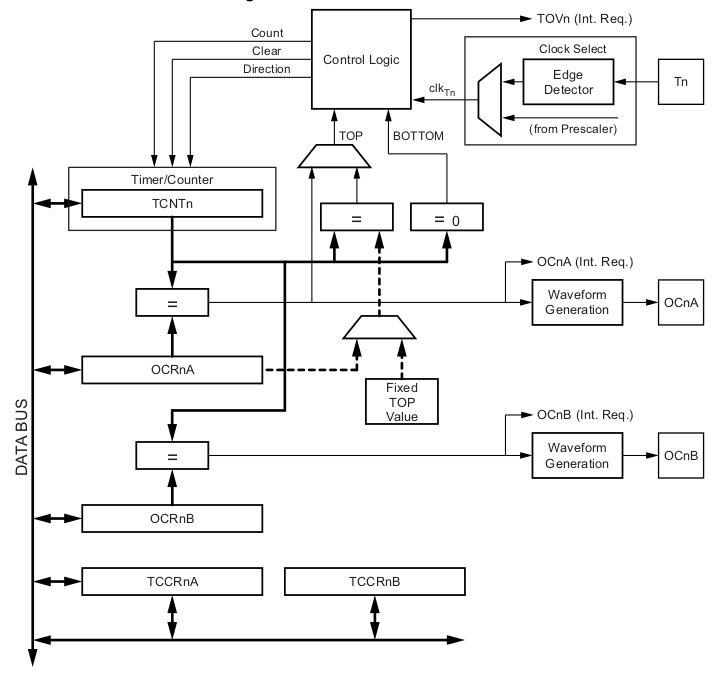
\includegraphics[height=0.6\textheight]{Timer0BlockDiagram.png}
    \end{center}
\end{figure}

\section{Terminologies and Registers}
\begin{minipage}{0.45\textwidth}
    \begin{tabular}{c|p{5.5cm}}
        \textbf{Parameter} & \textbf{Description}\\
        \hline
        BOTTOM & counter reaches 0x00\\
        MAX & ounter reaches 0xFF\\
        TOP & counter reaches highest value (depends on mode of operation can be 0xFF, OCR0A).        
    \end{tabular}
\end{minipage}
\begin{minipage}{0.5\textwidth}
    \begin{tabular}{c|p{6cm}}
        \textbf{Register - 8 bit} & \textbf{Name}\\
        \hline
        \regFormat{TCNT0} & Timer/Counter0 count value\\
        \regFormat{TCCR0A} & Timer/Coutner0 Control Register A\\
        \regFormat{TCCR0B} & Timer/Coutner0 Control Register B\\
        \regFormat{OCBR0A} & Output compare register A\\
        \regFormat{OCBR0B} & Output compare register B\\
        \regFormat{TIFR0} & Timer Interrupt Flag Register\\
        \regFormat{TIMSK0} & Timer interrupt Mask Register\\
    \end{tabular}
\end{minipage}

\section{Timer/Counter0 Units}
\subsection{Clock Source/Select Unit}
\begin{figure}[H]
    \begin{center}
        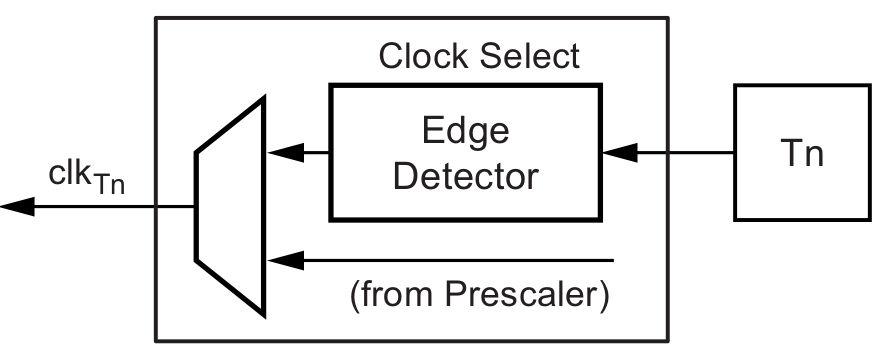
\includegraphics[width=0.5\textwidth]{Timer0ClockSelector.png}
    \end{center}
\end{figure}
\begin{itemize}
    \item The source for the Timer/Counter0 can be external or internal.
    \item External clock source is from \pinFormat{T0} pin.
    \item While Internal Clock source can be clocked via a prescalar.
    \item The output of this unit is the timer clock ($clk_{T0}$).
    \item It uses \bitFormat{CS0[2:0]} bits in \regFormat{TCCR0B} register to select the source.
\end{itemize}


\subsection{Counter Unit}
\begin{minipage}{0.5\textwidth}
    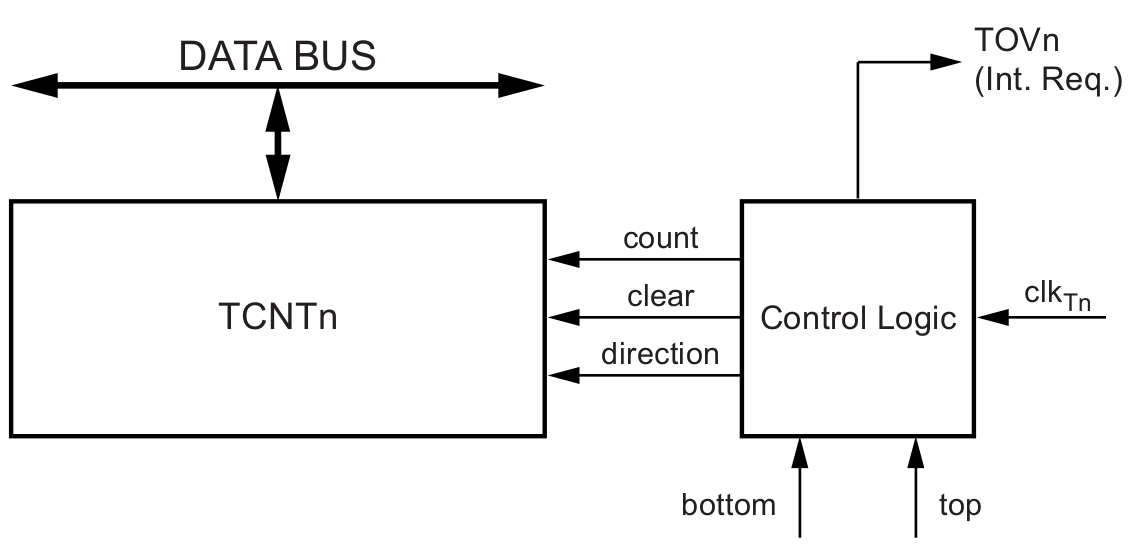
\includegraphics[width=1\textwidth]{Timer0CounterUnit.png}
\end{minipage}
\begin{minipage}{0.45\textwidth}
    \begin{tabular}{c|p{5.5cm}}
        \textbf{Signal} & \textbf{Description}\\
        \hline  
        count & Increment or decrement \regFormat{TCNT0} by 1\\
        direction & Select between increment or decrement\\
        clear & Clears \regFormat{TCNT0} to 0x00\\
        $clk_{T0}$ & Timer/Coutner0 clock\\
        top & Signalize that \regFormat{TCNT0} has maximum value\\
        bottom & Signalize that \regFormat{TCNT0} has minimum value(0x00)\\
    \end{tabular}
\end{minipage}
\begin{itemize}
    \item The main part of the 8-bit Timer/Counter is the programmable bi-directional counter.
    \item Depending the mode of operation the counter is cleared, incremented, or decremented at each timer clock ($clk_{T0}$).
    \item Counting sequence is determined by \bitFormat{WGM0[1:0]} bits of \regFormat{TCCR0A} -Timer/Counter0 Control register A and \bitFormat{WGM02} bit of \regFormat{TCCR0B} - Timer/Counter0 Control register B.
    \item The Timer/Counter0 Overflow flag \bitFormat{TOV0} is set and can generate interrupt according to the mode.
\end{itemize}


\subsection{Output Compare Unit}
\begin{figure}[H]
    \begin{center}
        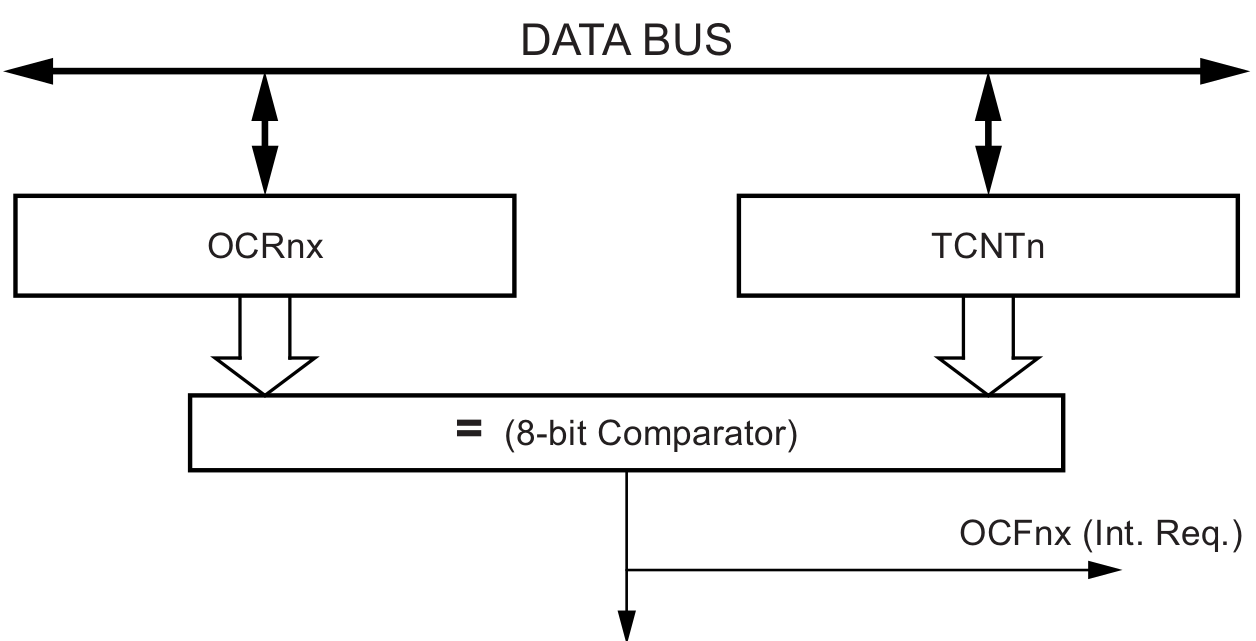
\includegraphics[width=0.5\textwidth]{Timer0CompareUnit.png}
    \end{center}
\end{figure}
\begin{itemize}
    \item 8-bit comparator continuously compares \regFormat{TCNT0} with both \regFormat{OCR0A} and \regFormat{OCR0B}.
    \item When \regFormat{TCNT0} equals \regFormat{OCR0A} or \regFormat{OCR0B}, the comparator signals a match which will set the output compare flag at the next timer clock cycle.
    \item If interrupts are enabled, then output compare interrupt is generated.
    \item The waveform generator uses the match signal to generate an output according to operating mode set by the \bitFormat{WGM0[2:0]} bits and compare output mode \bitFormat{COM0x[1:0]} bits.
\end{itemize}

\subsection{Compare Match Output Unit}
\begin{figure}[H]
    \begin{center}
        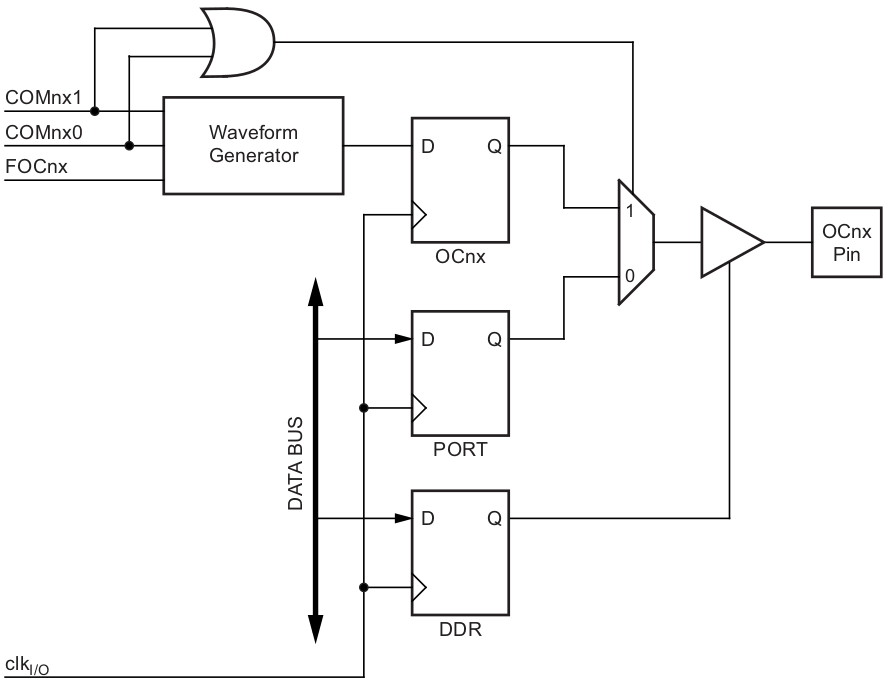
\includegraphics[height=0.3\textheight]{Timer0ComparteMatch.png}
    \end{center}
\end{figure}
\begin{itemize}
    \item This unit is used for changing the state of \pinFormat{OC0A} and \pinFormat{OC0B} pins by configuring the \bitFormat{COM0x[1:0]} bits.
    \item But, general I/O port function is overriiden by DDR reigster.
\end{itemize}

\section{Modes of Operation}
\begin{itemize}
    \item The mode of operation can be defined by combination of waveform generation mode (\bitFormat{WGM0[2:0]}) and compare output mode(\bitFormat{COM0[1:0]}) bits.
    \item The waveform generation mode (\bitFormat{WGM0[2:0]}) bits affect the counting sequence.
    \item For non-PWM mode, \bitFormat{COM0[1:0]} bits control if the output should be set, cleared or toggled at a compare match.
    \item For PWM mode, \bitFormat{COM0[1:0]} bits control if the PWM generated should be inverted or non-inverted.
\end{itemize}

\subsection{Normal Mode - Non-PWM Mode}
\begin{itemize}
    \item \bitFormat{WGM0[2:0]} $-->$ 000.
    \item Counter counts up and no counter clear.
    \item Overruns TOP(0XFF) and restarts from BOTTOM(0X00).
    \item \bitFormat{TOV0} Flag is only set when overrun.
    \item We have to clear \bitFormat{TOV0} flag inorder to have next running.
    \item But, if we use interrupt we don’t need to clear it as interrupt automatically clear the \bitFormat{TOV0} flag.
    \item The timing can be seen below.
\end{itemize}

\begin{tikztimingtable}[
    timing/dslope=0.1,
    timing/.style={x=5ex,y=2ex},
    x=5ex,
    timing/rowdist=3ex,
    timing/name/.style={font=\sffamily\scriptsize}
    ]
    \busref{clk\_{T0}}  & 41{c}\\
    \busref{TCNT0} & u{} D{0x00} D{0x01};[dotted] 2D{};D{0xFE} D{0xFF}D{0x00} D{0x01};[dotted] 2D{};D{0xFE} D{0xFF}D{0x00} D{0x01};[dotted] 2D{};D{0xFE} D{0xFF}D{0x00} D{0x01}\\
    \busref{TOV0} & l 6{L} H 5{L} H 5{L} H 1{L}\\
\end{tikztimingtable}

\subsection{Clear Timer on Compare Match(CTC) Mode - Non-PWM Mode}
\begin{itemize}
    \item \bitFormat{WGM0[2:0]} $-->$ 010.
    \item Counter value clears when \regFormat{TCNT0} reaches \regFormat{OCR0A}.
    \item Interrupt can be generated each time \regFormat{TCNT0} reaches \regFormat{OCR0A} register value by \bitFormat{OCF0A} flag.
    \item When \bitFormat{COM0A[1:0]} == 01, the \pinFormat{OC0A} pin output can be set to toggle its match between \regFormat{TCNT0} and \regFormat{OCR0A} to generate waveform.
    \item The frequency of the waveform its
    \begin{center}
        { \Large $f_{OC0A} = \frac{f_{clkT0}}{2 * N * (1 + OCR0A)}$ }
    \end{center}
    \item Here N is prescalar factor and can be (1, 8, 64, 256, or 1024).
\end{itemize}
\begin{tikztimingtable}[
    timing/dslope=0.1,
    timing/.style={x=5ex,y=2ex},
    x=5ex,
    timing/rowdist=3ex,
    timing/name/.style={font=\sffamily\scriptsize}
    ]
    \busref{clk\_{T0}}  & 28{1.5c}\\
    \busref{TCNT0} & 0.75U{} 1.5D{0x00} 1.5D{0x01};[dotted] 3D{};1.5D{OCR0A - 1} 1.5D{OCR0A}1.5D{0x00} 1.5D{0x01};[dotted] 3D{};1.5D{OCR0A - 1} 1.5D{OCR0A} 1.5D{0x00} 0.75D{0x01} \\
    \busref{OC0A} & 0.75L 9{L} 1.5H l 7{L} 1.5H l\\
\end{tikztimingtable}

\subsection{Fast PWM Mode}
\begin{itemize}
    \item \bitFormat{WGM0[2:0]} $-->$ 011 or 111.
    \item Power Regulation, Rectification, DAC applications.
    \item Single slope operations causing high frequency PWM waveform.
    \item Counter starts from BOTTOM to TOP and then restarts from BOTTOM.
    \item TOP is defined by
    \begin{itemize}
        \item TOP == 0xFF if \bitFormat{WGM0[2:0]} $-->$ 011
        \item TOP == \regFormat{OCR0A} if \bitFormat{WGM0[2:0]} $-->$ 111
    \end{itemize}
    \item  When \bitFormat{COM0A[1:0]} == 01, the \pinFormat{OC0A} pin output can be set to toggle its match between \regFormat{TCNT0} and TOP to generate waveform.
    \begin{itemize}
        \item The above is possible only when \bitFormat{WGM02} bit is set.
        \item And only on \pinFormat{OC0A} pin and not on \pinFormat{OC0B} pin.
    \end{itemize}
    \item In Inverting Compare Mode \bitFormat{COM0A[1:0]} == 10 , the \pinFormat{OC0A} or \pinFormat{OC0B} pins is made 1 on compare match between \regFormat{TCNT0} and TOP and made 0 on reaching BOTTOM.
    \item In Non-Inverting Compare Mode \bitFormat{COM0A[1:0]} == 11 , the \pinFormat{OC0A} or \pinFormat{OC0B} pins is made 0 on compare match between \regFormat{TCNT0} and TOP and 1 made  on reaching BOTTOM.
    \item The Timer/Counter overflow flag (\bitFormat{TOV0}) is set each time the counter reaches TOP.
    \item The PWM frequency is given by 
    \begin{center}
        { \Large $f_{OC0xPWM} = \frac{f_{clkT0}}{N * 256}$ }
    \end{center}
\end{itemize}

\subsubsection{WGM[2:0] == 011}
\begin{tikztimingtable}[
    timing/dslope=0.1,
    timing/.style={x=5ex,y=2ex},
    x=5ex,
    timing/rowdist=3ex,
    timing/name/.style={font=\sffamily\scriptsize}
    ]
    \busref{clk\_{T0}}  & 41{1c} c\\
    \busref{TCNT0} & 0.5U{} D{0x00} 1D{0x01};[dotted] 1.5D{};1D{0xFE} 1D{0xFF}1D{0x00} 1D{0x01};[dotted] 1D{};1D{0xFE} 1D{0xFF} 1D{0x00} 1D{0x01} [dotted] 1D{};1D{0xFE} 1D{0xFF} 1D{0x00} 1D{0x01};[dotted] 1D{};1D{0xFE} 1D{0xFF};\\
    \busref{TOV0} & 6{L} H 4{L} H 4{L} H 4{L} \\
\end{tikztimingtable}

\subsubsection{WGM[2:0] == 011}
\begin{tikztimingtable}[
    timing/dslope=0.1,
    timing/.style={x=5ex,y=2ex},
    x=5ex,
    timing/rowdist=3ex,
    timing/name/.style={font=\sffamily\scriptsize}
    ]
    \busref{clk\_{T0}}  & 41{1c} c\\
    \busref{TCNT0} & 0.5U{} D{0x00} 1D{0x01};[dotted] 1.5D{};1D{\tiny OCR0A -1} 1D{\tiny OCR0A}1D{0x00} 1D{0x01};[dotted] 1D{};1D{\tiny OCR0A -1} 1D{\tiny OCR0A} 1D{0x00} 1D{0x01} [dotted] 1D{};1D{\tiny OCR0A -1} 1D{\tiny OCR0A} 1D{0x00} 1D{0x01};[dotted] 1D{};1D{\tiny OCR0A -1} 1D{\tiny OCR0A};\\
    \busref{TOV0} & 6{L} H 4{L} H 4{L} H 4{L} \\
\end{tikztimingtable}


\subsection{Phase Correct PWM Mode}
\begin{itemize}
    \item \bitFormat{WGM0[2:0]} $-->$ 001 or 101.
    \item High resolution phase correct PWM.
    \item Motor control due to symmetric features
    \item Dual slope operations causing ower frequency PWM waveform.
    \item Counter starts from BOTTOM to TOP and then from TOP to BOTTOM.
    \item TOP is defined by
    \begin{itemize}
        \item TOP == 0xFF if \bitFormat{WGM0[2:0]} $-->$ 001
        \item TOP == \regFormat{OCR0A} if \bitFormat{WGM0[2:0]} $-->$ 101
    \end{itemize}
    \item  When \bitFormat{COM0A[1:0]} == 01, the \pinFormat{OC0A} pin output can be set to toggle its match between \regFormat{TCNT0} and TOP to generate waveform.
    \begin{itemize}
        \item The above is possible only when \bitFormat{WGM02} bit is set.
        \item And only on \pinFormat{OC0A} pin and not on \pinFormat{OC0B} pin.
    \end{itemize}
    \item In Inverting Compare Mode \bitFormat{COM0A[1:0]} == 10 , the \pinFormat{OC0A} or \pinFormat{OC0B} pins is made 1 on compare match between \regFormat{TCNT0} and TOP and made 0 on reaching BOTTOM.
    \item In Non-Inverting Compare Mode \bitFormat{COM0A[1:0]} == 11 , the \pinFormat{OC0A} or \pinFormat{OC0B} pins is made 0 on compare match between \regFormat{TCNT0} and TOP and 1 made  on reaching BOTTOM.
    \item The Timer/Counter overflow flag (\bitFormat{TOV0}) is set each time the counter reaches BOTTOM..
    \item The PWM frequency is given by 
    \begin{center}
        { \Large $f_{OC0xPWM} = \frac{f_{clkT0}}{N * 510}$ }
    \end{center}
\end{itemize}

\subsubsection{WGM[2:0] == 001}
\begin{tikztimingtable}[
    timing/dslope=0.1,
    timing/.style={x=5ex,y=2ex},
    x=5ex,
    timing/rowdist=3ex,
    timing/name/.style={font=\sffamily\scriptsize}
    ]
    \busref{clk\_{T0}}  & 41{1c}\\
    \busref{TCNT0} & 0.5U{} D{0x00} 1D{0x01};[dotted] 1.5D{};1D{0xFE} 1D{0xFF}1D{0xFE} 1D{0xFD};[dotted] 1D{};1D{0x01} 1D{0x00} 1D{0x01}[dotted] 1D{};1D{0xFE} 1D{0xFF} 1D{0xFE} 1D{0xFD};[dotted] 1D{};1D{0x01} 1D{0x00} 1d{0x01};\\
    \busref{TOV0} & l H l 8{L} H 8{L} H l\\
\end{tikztimingtable}

\subsubsection{WGM[2:0] == 101}
\begin{tikztimingtable}[
    timing/dslope=0.1,
    timing/.style={x=5ex,y=2ex},
    x=5ex,
    timing/rowdist=3ex,
    timing/name/.style={font=\sffamily\scriptsize}
    ]
    \busref{clk\_{T0}}  & 41{1c}\\
    \busref{TCNT0} & 0.5U{} D{0x00} 1D{0x01};[dotted] 1.5D{};1D{\tiny OCR0A - 1} 1D{\tiny OCR0A}1D{\tiny OCR0A-1} 1D{\tiny OCR0A-2};[dotted] 1D{};1D{0x01} 1D{0x00} 1D{0x01}[dotted] 1D{};1D{\tiny OCR0A-1} 1D{\tiny OCR0A} 1D{\tiny OCR0A-1} 1D{\tiny OCR0A-2};[dotted] 1D{};1D{0x01} 1D{0x00} 1d{0x01};\\
    \busref{TOV0} & l H l 8{L} H 8{L} H l\\
\end{tikztimingtable}
\newpage
\section{Register Description}
\subsubsection*{TCCR0A – Timer/Counter Control Register A}
\vspace*{0.5cm}
\begin{bytefield}[bitformatting={\large\bfseries},
    endianness=big,bitwidth=0.125\linewidth]{8}
    \bitheader[lsb=0]{0-7} \\
    \bitbox{1}{\small COM0A1}
    \bitbox{1}{\small COM0A0}
    \bitbox{1}{\small COM0B1}
    \bitbox{1}{\small COM0B0}
    \bitbox{1}{\small -}
    \bitbox{1}{\small -}
    \bitbox{1}{\small WGM01}
    \bitbox{1}{\small WGM00}\\
\end{bytefield}

\begin{table}[H]
    \begin{center}
        \begin{tabular}{c|p{4cm}|p{5.2cm}|p{5.2cm}}
            \bitFormat{COM0B[1:0]} & \textbf{Non-PWM modes} & \textbf{Fast PWM} & \textbf{Phase Corrected PWM}\\
            \hline
            00 & No output @ \pinFormat{PD5 - OC0B} pin &  No output @ \pinFormat{PD5 - OC0B} & No output @ \pinFormat{PD5 - OC0B}\\
            \hline
            01 & Toggle \pinFormat{PD5 - OC0B} pin on compare Match. & Reserved & Reserved\\
            \hline
            10 & Clear \pinFormat{PD5 - OC0B} pin on compare Match. & Clear \pinFormat{PD5 - OC0B} on compare match and  set \pinFormat{PD5 - OC0B} at BOTTOM & Clear \pinFormat{PD5 - OC0B} on compare match when up-counting and set \pinFormat{PD5 - OC0B} on compare match when down-counting.\\
            \hline
            11 & Set \pinFormat{PD5 - OC0B} pin on compare Match. & Set \pinFormat{PD5 - OC0B} on compare match and clear \pinFormat{PD5 - OC0B} at BOTTOM & Set \pinFormat{PD5 - OC0B} on compare match when up-counting and clear \pinFormat{PD5 - OC0B} on compare match when down-counting\\
        \end{tabular}
    \end{center}
\end{table}

\begin{table}[H]
    \begin{center}
        \begin{tabular}{c|p{4cm}|p{5.2cm}|p{5.2cm}}
            \bitFormat{COM0A[1:0]} & \textbf{Non-PWM modes} & \textbf{Fast PWM} & \textbf{Phase Corrected PWM}\\
            \hline
            00 & No output @ \pinFormat{PD6 - OC0A} pin &  No output @ \pinFormat{PD6 - OC0A} & No output @ \pinFormat{PD6 - OC0A}\\
            \hline
            01 & Toggle \pinFormat{PD6 - OC0A} pin on compare Match. & When WGM0[2] == 1, Toggle \pinFormat{PD6 - OC0A}  pin on Compare match & Toggle \pinFormat{PD6 - OC0A}  pin on Compare match\\
            \hline
            10 & Clear \pinFormat{PD6 - OC0A} pin on compare Match. & Clear \pinFormat{PD6 - OC0A} on compare match and  set \pinFormat{PD6 - OC0A} at BOTTOM & Clear \pinFormat{PD6 - OC0A} on compare match when up-counting and set \pinFormat{PD6 - OC0A} on compare match when down-counting.\\
            \hline
            11 & Set \pinFormat{PD6 - OC0A} pin on compare Match. & Set \pinFormat{PD6 - OC0A} on compare match and  clear \pinFormat{PD6 - OC0A} at BOTTOM & Set \pinFormat{PD6 - OC0A} on compare match when up-counting and clear \pinFormat{PD6 - OC0A} on compare match when down-counting\\
        \end{tabular}
    \end{center}
\end{table}

\begin{table}[H]
    \begin{center}
        \begin{tabular}{c|c|c|c}
            \bitFormat{WGM0[2:0]} & \textbf{Mode of operation} & \textbf{TOP} & \textbf{TOV0 Flag set on}\\
            \hline
            000 & Normal & 0xFF & MAX\\
            001 & PWM Phase Corrected & 0xFF & BOTTOM\\
            010 & CTC & OCRA & MAX\\
            011 & Fast PWM & 0xFF & MAX\\
            101 & PWM Phase Corrected & OCR0A  & BOTTOM\\
            111 & Fast PWM & OCR0A & TOP\\
        \end{tabular}
    \end{center}
\end{table}

\subsubsection*{TCCR0B – Timer/Counter Control Register B}
\vspace*{0.5cm}
\begin{bytefield}[bitformatting={\large\bfseries},
    endianness=big,bitwidth=0.125\linewidth]{8}
    \bitheader[lsb=0]{0-7} \\
    \bitbox{1}{\small FOC0A}
    \bitbox{1}{\small FOC0B}
    \bitbox{1}{\small -}
    \bitbox{1}{\small -}
    \bitbox{1}{\small WGM02}
    \bitbox{1}{\small CS02}
    \bitbox{1}{\small CS01}
    \bitbox{1}{\small CS00}\\
\end{bytefield}

\begin{table}[H]
    \begin{center}
        \begin{tabular}{c|c}
            \bitFormat{CS0[2:0]} & \textbf{Description(Prescalar)}\\
            \hline
            000 & No clock source(Timer/Counter Stopped)\\
            001 & $clk_{I/O}$ – no prescaling\\
            010 & $\frac{clk_{I/O}}{8}$\\
            011 & $\frac{clk_{I/O}}{64}$\\\
            100 & $\frac{clk_{I/O}}{256}$\\\
            101 & $\frac{clk_{I/O}}{1024}$\\\
            110 & External clock source on \pinFormat{T0} pin. Clock on falling edge.\\
            111 & External clock source on \pinFormat{T0} pin. Clock on rising edge.\\
        \end{tabular}
    \end{center}
\end{table}

\subsubsection*{TIMSK0 – Timer/Counter Interrupt Mask Register}
\vspace*{0.5cm}
\begin{bytefield}[bitformatting={\large\bfseries},
    endianness=big,bitwidth=0.125\linewidth]{8}
    \bitheader[lsb=0]{0-7} \\
    \bitbox{1}{\small -}
    \bitbox{1}{\small -}
    \bitbox{1}{\small -}
    \bitbox{1}{\small -}
    \bitbox{1}{\small -}
    \bitbox{1}{\small OCIE0B}
    \bitbox{1}{\small OCIE0A}
    \bitbox{1}{\small TOIE0}\\
\end{bytefield}

\quad Enable interrupts for compare match between \regFormat{TCNT0} and \regFormat{OCR0A} or \regFormat{TCNT0} and \regFormat{OCR0B} or overflow in \regFormat{TCNT}0.

\subsubsection*{TIFR0 – Timer/Counter 0 Interrupt Flag Register}
\vspace*{0.5cm}
\begin{bytefield}[bitformatting={\large\bfseries},
    endianness=big,bitwidth=0.125\linewidth]{8}
    \bitheader[lsb=0]{0-7} \\
    \bitbox{1}{\small -}
    \bitbox{1}{\small -}
    \bitbox{1}{\small -}
    \bitbox{1}{\small -}
    \bitbox{1}{\small -}
    \bitbox{1}{\small OCIE0B}
    \bitbox{1}{\small OCIE0A}
    \bitbox{1}{\small TOIE0}\\
\end{bytefield}

\quad FLag registers for interrupts on compare match between \regFormat{TCNT0} and \regFormat{OCR0A} or \regFormat{TCNT0} and \regFormat{OCR0B} or overflow in \regFormat{TCNT0}.
\newpage


\section{Configuring the Timer/Counter}
\subsection{Normal Mode}
\subsubsection{As Timer}
\begin{center}
    $ON\_TIME = \frac{max\_count}{\frac{F\_CPU}{PRESCALAR}}$
\end{center}
\begin{itemize}
    \item Depending on PRESCALR value, we get different ON\_TIME.
    \item First, \bitFormat{WGM0[2:0]} bits are configured as 000 for Normal Mode in \regFormat{TCCR0A} and \regFormat{TCCR0B} registers.
    \item Next, \bitFormat{COM0A[1:0]} and/or \bitFormat{COM0A[1:0]} bits are configured to make outputs \pinFormat{OC0A} and/or \pinFormat{OC0B} pins to do nothing, set, clear or toggle in \regFormat{TCCR0A} register.
    \item Next, Interrupt is Enabled by \bitFormat{TOIE0} (overflow enable) in \regFormat{TIMSK0} reigster.
    \item Finally, Timer is started by setting prescalar in \bitFormat{CS0[2:0]} bits as needed prescalar of \regFormat{TCR0B} reigster.
    \item Global Interrupt is enabled.
    \item A interrupt Service Routine for Timer0 overflow is Written.
    \item No need to clear the overflow flag as it is done by hardware.
    \item The timing when both pins \pinFormat{OC0A} and \pinFormat{OC0B} are made to toggle.
\end{itemize}

\begin{tikztimingtable}[
    timing/dslope=0.1,
    timing/.style={x=5ex,y=2ex},
    x=5ex,
    timing/rowdist=3ex,
    timing/name/.style={font=\sffamily\scriptsize}
    ]
    \busref{clk\_{T0}}  & 41{c}\\
    \busref{TCNT0} & u{} D{0x00} D{0x01};[dotted] 2D{};D{0xFE} D{0xFF}D{0x00} D{0x01};[dotted] 2D{};D{0xFE} D{0xFF}D{0x00} D{0x01};[dotted] 2D{};D{0xFE} D{0xFF}D{0x00} D{0x01}\\
    \busref{TOV0} & u h h 5{L} H 5{L} H 5{L} H 1{L}\\
    \busref{OC0A} & l H 5{H} 6{L} 6{H} 2{L}\\
    \busref{OC0B} & h L 5{L} 6{H} 6{L} 2{H}\\
\end{tikztimingtable}
\begin{itemize}
    \item The code can be seen below,
\end{itemize}
\begin{minted}[breaklines,bgcolor=lightgray]{c}
// MOde of operation to Normal Mode -- WGM0[2:0] === 000
// WGM0[2](bit3) from TCCR0B, WGM0[1](bit1)  from TCCR0A, WGM0[0](bit0)  from TCCR0A
TCCR0A = TCCR0A & (~(1<<0) & ~(1<<1));
TCCR0B = TCCR0B & ~(1<<3);

/* What to do when timer reaches the MAX(0xFF) value */	
// toggle OC0A and OC0B on each time when reaches the MAX(0xFF) 
// which is reflected in PD6 and PD5

// Output OC0A to toglle when reaches MAX -- COM0A[1:0] === 01
// COM0A[1](bit7) from TCCR0A, COM0A[0](bit6) from TCCR0A
TCCR0A = TCCR0A & ~(1<<7);
TCCR0A = TCCR0A | (1<<6);

// Output OC0B to toglle when reaches MAX -- COM0B1:0] === 01
// COM0B[1](bit7) from TCCR0A, COM0B[0](bit6) from TCCR0A
TCCR0A = TCCR0A & ~(1<<5);
TCCR0A = TCCR0A | (1<<4);

//Enable Interrupt of OVERFLOW flag so that interrupt can be generated
TIMSK0 = TIMSK0 | (1<<0);	

// start timer by setting the clock prescalar
// DIVIDE BY 8 from I/O clock
// DIVIDE BY 8-- CS0[2:0] === 010
// CS0[2](bit2) from TCCR0B,CS0[1](bit1) from TCCR0B,CS0[0](bit0) from TCCR0B
TCCR0B = TCCR0B | (1<<1);
TCCR0B = TCCR0B & (~(1<<0) & ~(1<<2));

// enabling global interrupt
sei();
// SO ON TIME = max_count / (F_CPU / PRESCALAR)
// ON TIME = 0xFF / (16000000/8) = 128us
// since symmetric as toggling OFF TIME = 128us
// hence, we get a square wave of fequency 1 / 256us = 3.906kHz
\end{minted}

\begin{minted}[breaklines,bgcolor=lightgray]{c}
ISR(TIMER0_OVF_vect)
{
    // do the thing when overflows.
}
\end{minted}


\subsubsection{As Counter}
\begin{itemize}
    \item Every rising/falling edge the count increases.
    \item So to reach 256 count, it would take a time of $\frac{0xFF}{frequency @ \pinFormat{T0} pin}$.
    \item First, \bitFormat{WGM0[2:0]} bits are configured as 000 for Normal Mode in \regFormat{TCCR0A} and \regFormat{TCCR0B} registers.
    \item Finally, Counter is started by configuring \bitFormat{CS0[2:0]} bits to 110 or 111 for external falling or rising edge on \pinFormat{T0 - PD4}.
    \item The code when \pinFormat{T0} pin is used as counter @ falling edge.
\end{itemize}

\begin{minted}[breaklines,bgcolor=lightgray]{c}
// MOde of operation to Normal Mode -- WGM0[2:0] === 000
// WGM0[2](bit3) from TCCR0B, WGM0[1](bit1)  from TCCR0A, WGM0[0](bit0)  from TCCR0A
TCCR0A = TCCR0A & (~(1<<0) & ~(1<<1));
TCCR0B = TCCR0B & ~(1<<3);
    
/* to count external event -we must connect source to T0 (PD4) */
// THE CLK IS CLOCKED FROM external source
// Falling edge of T0(PD4) -- CS0[2:0] === 110
// CS0[2](bit2) from TCCR0B,CS0[1](bit1) from TCCR0B,CS0[0](bit0) from TCCR0B
TCCR0B = TCCR0B | (1<<2);
TCCR0B = TCCR0B | (1<<1);
TCCR0B = TCCR0B & ~(1<<0);	
\end{minted}

\subsubsection{Application I - Delay}
\begin{minted}[breaklines,bgcolor=lightgray]{c}
/* TCNT0 starts from 0X00 goes upto 0XFF and restarts */
/* No possible use case as it just goes upto 0xFF and restarts */
// MOde of operation to Normal Mode -- WGM0[2:0] === 000
// WGM0[2](bit3) from TCCR0B, WGM0[1](bit1)  from TCCR0A, WGM0[0](bit0)  from TCCR0A
TCCR0A = TCCR0A & (~(1<<0) & ~(1<<1));
TCCR0B = TCCR0B & ~(1<<3);

/* What to do when timer reaches the MAX(0xFF) value */
// nothing should be done on OC0A for delay
// nothing  -- COM0A[1:0] === 00
// COM0A[1](bit7) from TCCR0A, COM0A[0](bit6) from TCCR0A
TCCR0A = TCCR0A & ~(1<<7);
TCCR0A = TCCR0A & ~(1<<6);
    
/* The delay possible = 0xff / (F_CPU/prescalar) */
// lowest delay = 0xff / (16000000 / 1) = 16us
// when prescalar == 8 --> delay = 0xff / (16000000 / 8) = 128us
// when prescalar == 64 --> delay = 0xff / (16000000 / 64) = 1.024ms
// when prescalar == 256 --> delay = 0xff / (16000000 / 256) = 4.096ms
// highest delay possible = 0xff / (16000000 / 1024) = 16.38ms

// start timer by setting the clock prescalar
// DIVIDE BY 8 use the same clock from I/O clock
// DIVIDE BY 8-- CS0[2:0] === 010
// CS0[2](bit2) from TCCR0B,CS0[1](bit1) from TCCR0B,CS0[0](bit0) from TCCR0B
TCCR0B = TCCR0B & ~(1<<0);
TCCR0B = TCCR0B | (1<<1);
TCCR0B = TCCR0B & ~(1<<2);


// actual delaying - wait until delay happens
while((TIFR0 & 0x01) == 0x00); // checking overflow flag when overflow happns
// clearing the overflag so that we can further utilize
TIFR0 = TIFR0 | 0x01;
\end{minted}

\subsection{CTC Mode}
\subsubsection{As Timer}

\begin{center}
    $ON\_TIME = \frac{1 + OCR0A}{\frac{F\_CPU}{PRESCALAR}}$
\end{center}
\begin{itemize}
    \item Depending on \regFormat{OCR0A} register and PRESCALR value, we get different ON\_TIME.
    \item First, \bitFormat{WGM0[2:0]} bits are configured as 010 for CTC Mode in \regFormat{TCCR0A} and \regFormat{TCCR0B} registers.
    \item Next, \bitFormat{COM0A[1:0]} and/or \bitFormat{COM0B[1:0]} bits are configured to make outputs \pinFormat{OC0A} and/or \pinFormat{OC0B} pins to do nothing, set, clear or toggle in \regFormat{TCCR0A} register.
    \item Next, Interrupt is Enabled by \bitFormat{OCIE01A} (utput compare on match on \regFormat{OCR0A} register enable) in \regFormat{TIMSK0} reigster.
    \item Finally, Timer is started by setting prescalar in \bitFormat{CS0[2:0]} bits as needed prescalar of \regFormat{TCR0B} reigster.
    \item Global Interrupt is enabled.
    \item A interrupt Service Routine for Timer0 Compare is Written.
    \item No need to clear the overflow flag as it is done by hardware.
    \item The timing when both pins \pinFormat{OC0n} are made to toggle.
\end{itemize}


\begin{tikztimingtable}[
    timing/dslope=0.1,
    timing/.style={x=5ex,y=2ex},
    x=5ex,
    timing/rowdist=3ex,
    timing/name/.style={font=\sffamily\scriptsize}
    ]
    \busref{clk\_{T0}}  & 41{c}\\
    \busref{TCNT0} & u{} D{0x00} D{0x01};[dotted] 2D{};D{\tiny OCR0A - 1} D{\tiny OCR0A}D{0x00} D{0x01};[dotted] 2D{};D{\tiny OCR0A - 1} D{\tiny OCR0A }D{0x00} D{0x01};[dotted] 2D{};D{\tiny OCR0A - 1} D{\tiny OCR0A}D{0x00} D{0x01}\\
    \busref{TOV0} & u h h 5{L} H 5{L} H 5{L} H 1{L}\\
    \busref{OC0A} & l H 5{H} 6{L} 6{H} 2{L}\\
    \busref{OC0B} & h L 5{L} 6{H} 6{L} 2{H}\\
\end{tikztimingtable}
\begin{itemize}
    \item The code can be seen below,
\end{itemize}
\begin{minted}[breaklines,bgcolor=lightgray]{c}
// MOde of operation to CTC Mode -- WGM0[2:0] === 010
// WGM0[2](bit3) from TCCR0B, WGM0[1](bit1)  from TCCR0A, WGM0[0](bit0)  from TCCR0A
TCCR0A = TCCR0A & ~(1<<0);
TCCR0A = TCCR0A | (1<<1);
TCCR0B = TCCR0B & ~(1<<3);

/* What to do when timer reaches the OCR0A */
// toggle OC0A on each time when reaches the OCR0A
// which is reflected in PD6
// Output OC0A to toglle when reaches MAX -- COM0A[1:0] === 01
// COM0A[1](bit7) from TCCR0A, COM0A[0](bit6) from TCCR0A
TCCR0A = TCCR0A & ~(1<<7);
TCCR0A = TCCR0A | (1<<6);

// Output OC0B to toglle when reaches MAX -- COM0B1:0] === 01
// COM0B[1](bit7) from TCCR0A, COM0B[0](bit6) from TCCR0A
TCCR0A = TCCR0A & ~(1<<5);
TCCR0A = TCCR0A | (1<<4);

    
// Enable Interrupt when counter matches OCR0A Rgister
//  OCIE0A bit is enabled
TIMSK0 = TIMSK0 | (1<<1);


// setting the value till the counter should reach in OCR0A
// for toggling of OC0A pin
OCR0A = 0x32;

// start timer by setting the clock prescalar
// DIVIDE BY 8 from I/O clock
// DIVIDE BY 8-- CS0[2:0] === 010
// CS0[2](bit2) from TCCR0B,CS0[1](bit1) from TCCR0B,CS0[0](bit0) from TCCR0B
TCCR0B = TCCR0B | (1<<1);
TCCR0B = TCCR0B & (~(1<<0) & ~(1<<2));

// enabling global interrupt
sei();
// SO ON TIME = (1 + OCR0A) / (F_CPU / PRESCALAR)
// ON TIME = 0X32 / (16000000/8) = 25.5us
// since symmetric as toggling OFF TIME = 25.5us
// hence, we get a square wave of fequency 1 / 50us = 20kHz
\end{minted}

\begin{minted}[breaklines,bgcolor=lightgray]{c}
ISR(TIMER0_COMPA_vect)
{
    // do the thing when compare match between TCNT0 matches OCR0A.
}
\end{minted}


\subsubsection{As Counter}
\begin{itemize}
    \item Every rising/falling edge the count increases.
    \item So to reach required count, it would take a time of $\frac{OCR0A}{frequency @ \pinFormat{T0} pin}$.
    \item First, \bitFormat{WGM0[2:0]} bits are configured as 010 for CTC Mode in \regFormat{TCCR0A} and \regFormat{TCCR0B} registers.
    \item Finally, Counter is started by configuring \bitFormat{CS0[2:0]} bits to 110 or 111 for external falling or rising edge on \pinFormat{T0 - PD4} pin.
    \item The code when \pinFormat{T0} pin is used as counter @ falling edge.
\end{itemize}

\begin{minted}[breaklines,bgcolor=lightgray]{c}
// MOde of operation to CTC Mode -- WGM0[2:0] === 010
// WGM0[2](bit3) from TCCR0B, WGM0[1](bit1)  from TCCR0A, WGM0[0](bit0)  from TCCR0A
TCCR0A = TCCR0A & ~(1<<0);
TCCR0A = TCCR0A | (1<<1);
TCCR0B = TCCR0B & ~(1<<3);
    
// Disbale Interrupt when counter matches OCR0A Rgister
//  OCIE0A bit is disabled
TIMSK0 = TIMSK0 & ~(1<<1);

//we count till OCR0A register value and reset and continue 
OCR0A = 0xA;

/* to count external event -we must connect source to T0 (PD4) */
// THE CLK IS CLOCKED FROM external source
// Falling edge of T0(PD4) -- CS0[2:0] === 110
// CS0[2](bit2) from TCCR0B,CS0[1](bit1) from TCCR0B,CS0[0](bit0) from TCCR0B
TCCR0B = TCCR0B | (1<<2);
TCCR0B = TCCR0B | (1<<1);
TCCR0B = TCCR0B & ~(1<<0);
\end{minted}

\subsubsection{Application I - Delay in ms}

\begin{minted}[bgcolor=lightgray]{c}
// minimum delay being 4us -- choose like that
// use PRESCALAR OF 1 -- 3us - 16us -- usage 3us - 16us -- factor=0 -- CS0[2:0]=1
// use PRESCALAR OF 8 -- 3us - 128us -- usage 17us - 128us -- factor=3 -- CS0[2:0]=2
// use PRESCALAR OF 64 -- 4us - 1.024ms -- usage 129us - 1024us -- factor=6 -- CS0[2:0]=3
// use PRESCALAR OF 256 -- 16us - 4.096ms -- usage 1025us - 4096us -- factor=8 -- CS0[2:0]=4
    
// MOde of operation to ctc Mode -- WGM0[2:0] === 010
// WGM0[2](bit3) from TCCR0B, WGM0[1](bit1)  from TCCR0A, WGM0[0](bit0)  from TCCR0A
TCCR0A = TCCR0A & ~(1<<0);
TCCR0A = TCCR0A | (1<<1);
TCCR0B = TCCR0B & ~(1<<3);

while(delayInMs--)
{
    // for 1ms delay
    OCR0A = 249;
    // start timer by setting the clock prescalar
    //  dived by 64 from I/O clock
    //  CS0[2:0] === 011
    // CS0[2](bit2) from TCCR0B,CS0[1](bit1) from TCCR0B,CS0[0](bit0) from TCCR0B
    TCCR0B = TCCR0B | (1<<0);
    TCCR0B = TCCR0B | (1<<1);
    TCCR0B = TCCR0B & ~(1<<2);

    // actual delaying - wait until delay happens
    while((TIFR0 & 0x02) == 0x00); // checking OCF0A (compare match flag A) flag when match happns
    // clearing the compare match flag so that we can further utilize
    TIFR0 = TIFR0 | 0x02;
}
\end{minted}

\subsection{Fast PWM Mode}
\begin{minted}[bgcolor=lightgray]{c}
ISR(TIMER0_OVF_vect)
{
} 
ISR(TIMER0_COMPA_vect)
{
}
ISR(TIMER0_COMPB_vect)
{
}
\end{minted}
\subsubsection{Non-Inverting  PWM with TOP at MAX(0xFF)}
\quad Frequency is chosen by PRESCALAR and Duty cycle by \regFormat{OCR0A} and/or \regFormat{OCR0B} register.
\begin{itemize}
    \item First, \bitFormat{WGM0[2:0]} bits are configured as 011 for Fast PWM Mode with TOP at MAX in \regFormat{TCCR0A} and \regFormat{TCCR0B} registers.
    \item Next, \bitFormat{COM0A[1:0]} and/or \bitFormat{COM0B[1:0]} bits of \regFormat{TCCR0A} register are configured to make outputs \pinFormat{OC0A} and/or \pinFormat{OC0B} pins to generate PWM by comparing between \regFormat{OCR0A} and/or \regFormat{OCR0B} respectively. That is for Non-Inverting, \bitFormat{COM0x[1:0]} is written 10.
    \item Next, the duty cycle value is loaded into \regFormat{OCR0A} and/or \regFormat{OCR0B} register for \pinFormat{OC0A} and/or \pinFormat{OC0B} pins.
    \item Also, the \bitFormat{OCIE0A} and/or \bitFormat{OCIE0B} bits of \regFormat{TIMSK0} register  are enabled for Output Compare Interupts if needed.
    \item The interrupt Service routine is written if needed for compare match.
    \item Finally, Timer is started by setting \bitFormat{CS0[2:0]} bit as needed prescalar in \regFormat{TCR0B} register.
    \item The timing for PWM on 10\% duty cycle \pinFormat{OC0A} and 75\% duty cycle\pinFormat{OC0B} pins are shown assuming .
    \begin{itemize}
        \item 0x19 for OCR0A.
        \item 0xC0 for OCR0B.
    \end{itemize}
\end{itemize}

\begin{tikztimingtable}[
    timing/dslope=0.1,
    timing/.style={x=5ex,y=2ex},
    x=5ex,
    timing/rowdist=3ex,
    timing/name/.style={font=\sffamily\scriptsize}
    ]
    \busref{clk\_{T0}}  & 41{1c} \\
    \busref{TCNT0} & 0.5U{} D{0x00} 1D{0x01};[dotted] 1.5D{};1D{0x19} 1D{0x1A} [dotted] 1.5D{}; 1D{0xC0} 1D{0xC1} [dotted] 1.5D{};1D{0xFF} 1D{0x00} D{0x01} ;[dotted] 1.5D{};1D{0x19} 1D{0x1A} [dotted] 1.5D{};1D{0xBF} 1d{0xC0}\\
    \busref{OC0A} & u H H H h l L L L L L L L l H H H h L L L L L\\
    \busref{OC0B} & u H H H h HHH h L L L L l H H H h HHH Hhl\\
\end{tikztimingtable}

\begin{minted}[bgcolor=lightgray]{c}
// MOde of operation to fast_pwm_top_max Mode -- WGM0[2:0] === 011
// WGM0[2](bit3) from TCCR0B, WGM0[1](bit1)  from TCCR0A, WGM0[0](bit0)  from TCCR0A
TCCR0A = TCCR0A | (1<<0);
TCCR0A = TCCR0A | (1<<1);
TCCR0B = TCCR0B & ~(1<<3);	

// here we set COM0A[1:0] as 10 for non-inverting
// here we set COM0B[1:0] as 10 for non-inverting

// which is reflected in PD6
// COM0A[1](bit7) from TCCR0A, COM0A[0](bit6) from TCCR0A
TCCR0A = TCCR0A | (1<<7);
TCCR0A = TCCR0A & ~(1<<6);

// which is reflected in PD65
// COM0B[1](bit5) from TCCR0A, COM0B[0](bit4) from TCCR0A
TCCR0A = TCCR0A | (1<<5);
TCCR0A = TCCR0A & ~(1<<4);

// Enable Interrupt when TCN0 overflows TOP - here 0xFF
//  TOV0 bit is enabled
TIMSK0 = TIMSK0 | (1<<0);

/* we use OCF0A flag - which is set at every time TCN0 reaches OCR0A 
here we clear led(PC1),  so that we obtain the PWM when TCN0 reaches OCR0A*/
TIMSK0 = TIMSK0 | (1<<1);
/* we use OCF0B flag - which is set at every time TCN0 reaches OCR0B 
here we clear led(PC2),  so that we obtain the PWM when TCN0 reaches OCR0B*/
TIMSK0 = TIMSK0 | (1<<2);


// Next we set values for OCR0A and OCR0B
// Since, TCNT0 goes till max(0xFF), we can choose OCR0A and OCR0B to any value below max(0xFFF)
OCR0A = 0x19; // for 10% duty clcle
OCR0B = 0xC0; // for 75% duty clcle


// start the timer by selecting the prescalr
//  use the same clock from I/O clock
//  CS0[2:0] === 001
// CS0[2](bit2) from TCCR0B,CS0[1](bit1) from TCCR0B,CS0[0](bit0) from TCCR0B
TCCR0B = TCCR0B | (1<<0);
TCCR0B = TCCR0B & ~(1<<1);
TCCR0B = TCCR0B & ~(1<<2);

//enabled global interrupt
sei();
\end{minted}

\subsubsection{Inverting PWM with TOP at MAX(0xFF)}
\quad Frequency is chosen by PRESCALAR and Duty cycle by \regFormat{OCR0A} and/or \regFormat{OCR0B} register.
\begin{itemize}
    \item First, \bitFormat{WGM0[2:0]} bits are configured as 011 for Fast PWM Mode with TOP at MAX in \regFormat{TCCR0A} and \regFormat{TCCR0B} registers.
    \item Next, \bitFormat{COM0A[1:0]} and/or \bitFormat{COM0B[1:0]} bits of \regFormat{TCCR0A} register are configured to make outputs \pinFormat{OC0A} and/or \pinFormat{OC0B} pins to generate PWM by comparing between \regFormat{OCR0A} and/or \regFormat{OCR0B} respectively. That is for Inverting, \bitFormat{COM0x[1:0]} is written 11.
    \item Next, the duty cycle value is loaded into \regFormat{OCR0A} and/or \regFormat{OCR0B} register for \pinFormat{OC0A} and/or \pinFormat{OC0B} bits.
    \item Also, the \bitFormat{OCIE0A} and/or \bitFormat{OCIE0B} bits of \regFormat{TIMSK0} register  are enabled for Output Compare Interupts if needed.
    \item The interrupt Service routine is written if needed for compare match.
    \item Finally, Timer is started by setting \bitFormat{CS0[2:0]} bit as needed prescalar in \regFormat{TCR0B} register.
    \item The timing for PWM on 10\% duty cycle \pinFormat{OC0A} and 75\% duty cycle \pinFormat{OC0B} pins are shown assuming .
    \begin{itemize}
        \item 0x19 for OCR0A.
        \item 0xC0 for OCR0B.
    \end{itemize}
\end{itemize}

\begin{tikztimingtable}[
    timing/dslope=0.1,
    timing/.style={x=5ex,y=2ex},
    x=5ex,
    timing/rowdist=3ex,
    timing/name/.style={font=\sffamily\scriptsize}
    ]
    \busref{clk\_{T0}}  & 41{1c} \\
    \busref{TCNT0} & 0.5U{} D{0x00} 1D{0x01};[dotted] 1.5D{};1D{0x19} 1D{0x1A} [dotted] 1.5D{}; 1D{0xC0} 1D{0xC1} [dotted] 1.5D{};1D{0xFF} 1D{0x00} D{0x01} ;[dotted] 1.5D{};1D{0x19} 1D{0x1A} [dotted] 1.5D{};1D{0xBF} 1d{0xC0}\\
    \busref{OC0A} & u LLLl h HHHHHHHh LLLl HHHHH\\
    \busref{OC0B} & u LLLl LLL l HHHH h LLL l LLL Llh\\
\end{tikztimingtable}
\begin{minted}[bgcolor=lightgray]{c}
// MOde of operation to fast_pwm_top_max Mode -- WGM0[2:0] === 011
// WGM0[2](bit3) from TCCR0B, WGM0[1](bit1)  from TCCR0A, WGM0[0](bit0)  from TCCR0A
TCCR0A = TCCR0A | (1<<0);
TCCR0A = TCCR0A | (1<<1);
TCCR0B = TCCR0B & ~(1<<3);	

// here we set COM0A[1:0] as 11 for inverting
// here we set COM0B[1:0] as 11 for inverting

// which is reflected in PD6
// COM0A[1](bit7) from TCCR0A, COM0A[0](bit6) from TCCR0A
TCCR0A = TCCR0A | (1<<7);
TCCR0A = TCCR0A | (1<<6);

// which is reflected in PD65
// COM0B[1](bit5) from TCCR0A, COM0B[0](bit4) from TCCR0A
TCCR0A = TCCR0A | (1<<5);
TCCR0A = TCCR0A | (1<<4);

// Enable Interrupt when TCN0 overflows TOP - here 0xFF
//  TOV0 bit is enabled
TIMSK0 = TIMSK0 | (1<<0);

/* we use OCF0A flag - which is set at every time TCN0 reaches OCR0A 
    here we clear led(PC1),  so that we obtain the PWM when TCN0 reaches OCR0A*/
TIMSK0 = TIMSK0 | (1<<1);
/* we use OCF0B flag - which is set at every time TCN0 reaches OCR0B 
    here we clear led(PC2),  so that we obtain the PWM when TCN0 reaches OCR0B*/
TIMSK0 = TIMSK0 | (1<<2);

        
// Next we set values for OCR0A and OCR0B
// Since, TCNT0 goes till max(0xFF), we can choose OCR0A and OCR0B to any value below max(0xFFF)
OCR0A = 0x19; // for 10% duty clcle
OCR0B = 0xC0; // for 75% duty clcle


// start the timer by selecting the prescalr
//  use the same clock from I/O clock
//  CS0[2:0] === 001
// CS0[2](bit2) from TCCR0B,CS0[1](bit1) from TCCR0B,CS0[0](bit0) from TCCR0B
TCCR0B = TCCR0B | (1<<0);
TCCR0B = TCCR0B & ~(1<<1);
TCCR0B = TCCR0B & ~(1<<2);

//enabled global interrupt
sei();
\end{minted}


\subsubsection{Non-Inverting PWM with TOP at  OCR0A}
\quad Frequency is chosen by \regFormat{OCR0A} and Duty cycle by \regFormat{OCR0B} register.
\begin{itemize}
    \item First, \bitFormat{WGM0[2:0]} bits are configured as 111 for Fast PWM Mode with \regFormat{OCR0A} at MAX in \regFormat{TCCR0A} and \regFormat{TCCR0B} registers.
    \item Next,  \bitFormat{COM0B[1:0]} bits of \regFormat{TCCR0A} register are configured to make output \pinFormat{OC0B} pins to generate PWM by comparing between \regFormat{TCNT0} and \ \regFormat{OCR0B}. That is for Non-Inverting, \bitFormat{COM0B[1:0]} is written 10.
    \item The frequency of duty cycle is loaded into \regFormat{OCR0A} register.
    \item Next, the duty cycle value is loaded into \regFormat{OCR0B} register for \pinFormat{OC0B} bits.
    \item Also, the \bitFormat{OCIE0B} bits of \regFormat{TIMSK0} register  are enabled for Output Compare Interupts if needed.
    \item The interrupt Service routine is written if needed for compare match.
    \item Finally, Timer is started by setting \bitFormat{CS0[2:0]} bit as needed prescalar in \regFormat{TCR0B} register.
    \item The timing for PWM on 85\% duty cycle(0x60)  \pinFormat{OC0B} pins are shown assuming .
    \begin{itemize}
        \item 0x70 for OCR0A.
        \item 0x60 for OCR0B.
    \end{itemize}
\end{itemize}

\begin{tikztimingtable}[
    timing/dslope=0.1,
    timing/.style={x=5ex,y=2ex},
    x=5ex,
    timing/rowdist=3ex,
    timing/name/.style={font=\sffamily\scriptsize}
    ]
    \busref{clk\_{T0}}  & 41{1c} \\
    \busref{TCNT0} & 0.5U{} D{0x00} D{0x01} [dotted] 2D{}; D{0x60} [dotted] .5D{}; D{0x70} D{0x00} D{0x01} [dotted] 2D{}; D{0x60} [dotted] .5D{}; D{0x70} D{0x00} D{0x01}[dotted] 2D{}; D{0x60} [dotted] .5D{};D{0x70} d{0x00}\\
    \busref{OC0B} & u H H H h  h L L l H H H h h LLl HH H  H LL l h\\
\end{tikztimingtable}

\begin{minted}[bgcolor=lightgray]{c}
// MOde of operation to fast_pwm_top_max Mode -- WGM0[2:0] === 111
// WGM0[2](bit3) from TCCR0B, WGM0[1](bit1)  from TCCR0A, WGM0[0](bit0)  from TCCR0A
TCCR0A = TCCR0A | (1<<0);
TCCR0A = TCCR0A | (1<<1);
TCCR0B = TCCR0B | (1<<3);	

// here we set COM0B[1:0] as 10 for non-inverting
// which is reflected in PD5
// COM0B[1](bit5) from TCCR0A, COM0B[0](bit4) from TCCR0A
TCCR0A = TCCR0A | (1<<5);
TCCR0A = TCCR0A & ~(1<<4);

// Next we set values for OCR0A and OCR0B
// Since, TCNT0 goes till OCR0A, we can choose OCR0B to any value below OCR0A
OCR0A = 0x70; // for freqeuncy
OCR0B = 0x60; // for pwm duty cylc

// start the timer by selecting the prescalr
//  use the same clock from I/O clock
//  CS0[2:0] === 001
// CS0[2](bit2) from TCCR0B,CS0[1](bit1) from TCCR0B,CS0[0](bit0) from TCCR0B
TCCR0B = TCCR0B | (1<<0);
TCCR0B = TCCR0B & ~(1<<1);
TCCR0B = TCCR0B & ~(1<<2);

//enabled global interrupt
sei();
\end{minted}

\subsubsection{Inverting PWM with TOP at  OCR0A}
\quad Frequency is chosen by \regFormat{OCR0A} and Duty cycle by \regFormat{OCR0B} register.
\begin{itemize}
    \item First, \bitFormat{WGM0[2:0]} bits are configured as 111 for Fast PWM Mode with \regFormat{OCR0A} at MAX in \regFormat{TCCR0A} and \regFormat{TCCR0B} registers.
    \item Next, \bitFormat{COM0B[1:0]} bits of \regFormat{TCCR0A} register are configured to make output \pinFormat{OC0B} pins to generate PWM by comparing between \regFormat{TCNT0} and \ \regFormat{OCR0B}. That is for Inverting, \bitFormat{COM0B[1:0]} is written 11.
    \item The frequency of duty cycle is loaded into \regFormat{OCR0A} register.
    \item Next, the duty cycle value is loaded into \regFormat{OCR0B} register for \pinFormat{OC0B} bits.
    \item Also, the \bitFormat{OCIE0B} bits of \regFormat{TIMSK0} register  are enabled for Output Compare Interupts if needed.
    \item The interrupt Service routine is written if needed for compare match.
    \item Finally, Timer is started by setting \bitFormat{CS0[2:0]} bit as needed prescalar in \regFormat{TCR0B} register.
    \item The timing for PWM on 85\% duty cycle \pinFormat{OC0B} pins are shown assuming .
    \begin{itemize}
        \item 0x70 for OCR0A.
        \item 0x60 for OCR0B.
    \end{itemize}
\end{itemize}

\begin{tikztimingtable}[
    timing/dslope=0.1,
    timing/.style={x=5ex,y=2ex},
    x=5ex,
    timing/rowdist=3ex,
    timing/name/.style={font=\sffamily\scriptsize}
    ]
    \busref{clk\_{T0}}  & 41{1c} \\
    \busref{TCNT0} & 0.5U{} D{0x00} D{0x01} [dotted] 2D{}; D{0x60} [dotted] .5D{}; D{0x70} D{0x00} D{0x01} [dotted] 2D{}; D{0x60} [dotted] .5D{}; D{0x70} D{0x00} D{0x01}[dotted] 2D{}; D{0x60} [dotted] .5D{};D{0x70} d{0x00}\\
    \busref{OC0B} & u L L L l  l H H h L L L l l HHh LL L  L HH h l\\
\end{tikztimingtable}

\begin{minted}[bgcolor=lightgray]{c}
// MOde of operation to fast_pwm_top_max Mode -- WGM0[2:0] === 111
// WGM0[2](bit3) from TCCR0B, WGM0[1](bit1)  from TCCR0A, WGM0[0](bit0)  from TCCR0A
TCCR0A = TCCR0A | (1<<0);
TCCR0A = TCCR0A | (1<<1);
TCCR0B = TCCR0B | (1<<3);	

// here we set COM0B[1:0] as 11 for inverting
// which is reflected in PD5
// COM0B[1](bit5) from TCCR0A, COM0B[0](bit4) from TCCR0A
TCCR0A = TCCR0A | (1<<5);
TCCR0A = TCCR0A | (1<<4);

// Next we set values for OCR0A and OCR0B
// Since, TCNT0 goes till OCR0A, we can choose OCR0B to any value below OCR0A
OCR0A = 0x70; // for freqeuncy
OCR0B = 0x60; // for pwm duty cylc

// start the timer by selecting the prescalr
//  use the same clock from I/O clock
//  CS0[2:0] === 001
// CS0[2](bit2) from TCCR0B,CS0[1](bit1) from TCCR0B,CS0[0](bit0) from TCCR0B
TCCR0B = TCCR0B | (1<<0);
TCCR0B = TCCR0B & ~(1<<1);
TCCR0B = TCCR0B & ~(1<<2);

//enabled global interrupt
sei();
\end{minted}


\subsubsection{Toggling mode square Wave} 
\quad Frequency is chosen by \regFormat{OCR0A} register.
\begin{itemize}
    \item First, \bitFormat{WGM0[2:0]} bits are configured as 111 for Fast PWM Mode with OCR0A at MAX in \regFormat{TCCR0A} and \regFormat{TCCR0B} registers.
    \item Next, \bitFormat{COM0A[1:0]} bits of \regFormat{TCCR0A} register are configured to make output \pinFormat{OC0A} pins to generate PWM by comparing between \regFormat{OCR0A}. That is for Toggling square wave \bitFormat{COM0A[1:0]} is written 01.
    \item The frequency of duty cycle is loaded into \regFormat{OCR0A} register.
    \item Also, the \bitFormat{OCIE0A} bits of \regFormat{TIMSK0} register  are enabled for Output Compare Interupts if needed.
    \item The interrupt Service routine is written if needed for compare match.
    \item Finally, Timer is started by setting \bitFormat{CS0[2:0]} bit as needed prescalar in \regFormat{TCR0B} register.
    \item The timing for squared wave on \pinFormat{OC0A} pins are shown assuming.
    \begin{itemize}
        \item 0x70 for OCR0A.
    \end{itemize}
\end{itemize}

\begin{tikztimingtable}[
    timing/dslope=0.1,
    timing/.style={x=5ex,y=2ex},
    x=5ex,
    timing/rowdist=3ex,
    timing/name/.style={font=\sffamily\scriptsize}
    ]
    \busref{clk\_{T0}}  & 41{1c} \\
    \busref{TCNT0} & 0.5U{} D{0x00} D{0x01} [dotted] 2D{}; D{0x60} [dotted] .5D{}; D{0x70} D{0x00} D{0x01} [dotted] 2D{}; D{0x60} [dotted] .5D{}; D{0x70} D{0x00} D{0x01}[dotted] 2D{}; D{0x60} [dotted] .5D{};D{0x70} d{0x00}\\
    \busref{OC0A} & u L L L l  l H H h L L L l l HHh LL L  L HH h l\\
\end{tikztimingtable}

\begin{minted}[bgcolor=lightgray]{c}
// MOde of operation to fast_pwm_top_max Mode -- WGM0[2:0] === 111
// WGM0[2](bit3) from TCCR0B, WGM0[1](bit1)  from TCCR0A, WGM0[0](bit0)  from TCCR0A
TCCR0A = TCCR0A | (1<<0);
TCCR0A = TCCR0A | (1<<1);
TCCR0B = TCCR0B | (1<<3);	

// here we set COM0B[1:0] as 01 for toggling of OC0A
// which is reflected in PD6
// COM0A[1](bit7) from TCCR0A, COM0A[0](bit6) from TCCR0A
TCCR0A = TCCR0A & ~(1<<7);
TCCR0A = TCCR0A | (1<<6);

// Next we set values for OCR0A and OCR0B
// Since, TCNT0 goes till OCR0A, we can choose OCR0B to any value below OCR0A
OCR0A = 0x70; // for freqeuncy

// start the timer by selecting the prescalr
//  use the same clock from I/O clock
//  CS0[2:0] === 001
// CS0[2](bit2) from TCCR0B,CS0[1](bit1) from TCCR0B,CS0[0](bit0) from TCCR0B
TCCR0B = TCCR0B | (1<<0);
TCCR0B = TCCR0B & ~(1<<1);
TCCR0B = TCCR0B & ~(1<<2);

//enabled global interrupt
sei();
\end{minted}

\subsubsection{Application I - PWM generation}
\begin{minted}[bgcolor=lightgray]{c}
void Timer0_FastPWMGeneration(uint32_t on_time_us, uint32_t off_time_us)
{
	uint32_t total_time = on_time_us + off_time_us;
		
	// MOde of operation to fast_pwm_top_max Mode -- WGM0[2:0] === 111
	// WGM0[2](bit3) from TCCR0B, WGM0[1](bit1)  from TCCR0A, WGM0[0](bit0)  from TCCR0A
	TCCR0A = TCCR0A | (1<<0);
	TCCR0A = TCCR0A | (1<<1);
	TCCR0B = TCCR0B | (1<<3);	

	// which is reflected in PD5
	// COM0B[1](bit5) from TCCR0A, COM0B[0](bit4) from TCCR0A
	TCCR0A = TCCR0A | (1<<5);
	TCCR0A = TCCR0A & ~(1<<4);
	
	if(total_time <=3)
	{
		// if total_time <= 3us -- so we stop clock
		
		OCR0A = 0;
		// start timer by setting the clock prescalar
		//  use the same clock from I/O clock
		//  CS0[2:0] === 001
		// CS0[2](bit2) from TCCR0B,CS0[1](bit1) from TCCR0B,CS0[0](bit0) from TCCR0B
		TCCR0B = TCCR0B & ~(1<<0);
		TCCR0B = TCCR0B & ~(1<<1);
		TCCR0B = TCCR0B & ~(1<<2);
	}
	else if((3 < total_time)  && (total_time <= 16))
	{
		OCR0A = ((total_time * 16) >> 0) - 1;
		OCR0B = ((on_time_us * 16) >> 0) - 1;
		// start timer by setting the clock prescalar
		//  use the same clock from I/O clock
		//  CS0[2:0] === 001
		// CS0[2](bit2) from TCCR0B,CS0[1](bit1) from TCCR0B,CS0[0](bit0) from TCCR0B
		TCCR0B = TCCR0B | (1<<0);
		TCCR0B = TCCR0B & ~(1<<1);
		TCCR0B = TCCR0B & ~(1<<2);
	}
	else if((16 < total_time)  && (total_time <= 128))
	{
		OCR0A = ((total_time * 16) >> 3) - 1;
		OCR0B = ((on_time_us * 16) >> 3) - 1;
		// start timer by setting the clock prescalar
		//  dived by 8 from I/O clock
		//  CS0[2:0] === 010
		// CS0[2](bit2) from TCCR0B,CS0[1](bit1) from TCCR0B,CS0[0](bit0) from TCCR0B
		TCCR0B = TCCR0B & ~(1<<0);
		TCCR0B = TCCR0B | (1<<1);
		TCCR0B = TCCR0B & ~(1<<2);
	}
	else if((128 < total_time)  && (total_time <= 1024))
	{
		OCR0A = ((total_time * 16) >> 6) - 1;
		OCR0B = ((on_time_us * 16) >> 6) - 1;
		// start timer by setting the clock prescalar
		//  dived by 64 from I/O clock
		//  CS0[2:0] === 011
		// CS0[2](bit2) from TCCR0B,CS0[1](bit1) from TCCR0B,CS0[0](bit0) from TCCR0B
		TCCR0B = TCCR0B | (1<<0);
		TCCR0B = TCCR0B | (1<<1);
		TCCR0B = TCCR0B & ~(1<<2);
		
	}
	else if((1024 < total_time)  && (total_time <= 4096))
	{
		OCR0A = ((total_time * 16) >> 8) - 1;
		OCR0B = ((on_time_us * 16) >> 8) - 1;
		// start timer by setting the clock prescalar
		//  divide by256 from I/O clock
		//  CS0[2:0] === 100
		// CS0[2](bit2) from TCCR0B,CS0[1](bit1) from TCCR0B,CS0[0](bit0) from TCCR0B
		TCCR0B = TCCR0B & ~(1<<0);
		TCCR0B = TCCR0B & ~(1<<1);
		TCCR0B = TCCR0B | (1<<2);
		
	}
	else if(total_time > 4096)
	{
		// dont' cross more than 4.096ms
	}
}
void PWMGeneration(double duty_cycle_percent,uint32_t freqeuncy)
{
	double total_time_us = (1000000.0/freqeuncy);	
	double on_time_us = (duty_cycle_percent/100.0) * total_time_us;
	if (on_time_us<1.0)
	{
		on_time_us = 1;
	}
	
	// max time = 4ms -- min freqency = 250 Hz
	//  min time = 4us -- max frequency = 250000 = 250khz
	Timer0_FastPWMGeneration(on_time_us, total_time_us - on_time_us);
}
\end{minted}


\subsection{Phase Corrected PWM Mode}
\begin{minted}[bgcolor=lightgray]{c}
ISR(TIMER0_OVF_vect)
{
} 
ISR(TIMER0_COMPA_vect)
{
}
ISR(TIMER0_COMPB_vect)
{
}
\end{minted}
\subsubsection{Non-Inverting PWM with TOP at MAX(0xFF)}
\quad Frequency is chosen by PRESCALAR and Duty cycle by \regFormat{OCR0A} and/or \regFormat{OCR0B} register.
\begin{itemize}
    \item First, \bitFormat{WGM0[2:0]} bits are configured as 001 for Phase Corrected PWM Mode with TOP at MAX in \regFormat{TCCR0A} and \regFormat{TCCR0B} registers.
    \item Next, \bitFormat{COM0A[1:0]} and/or \bitFormat{COM0B[1:0]} bits of \regFormat{TCCR0A} register are configured to make outputs \pinFormat{OC0A} and/or \pinFormat{OC0B} pins to generate PWM by comparing between \regFormat{OCR0A} and/or \regFormat{OCR0B} respectively. That is for Non-Inverting, \bitFormat{COM0x[1:0]} is written 10.
    \item Next, the duty cycle value is loaded into \regFormat{OCR0A} and/or \regFormat{OCR0B} register for \pinFormat{OC0A} and/or \pinFormat{OC0B} bits.
    \item Also, the \bitFormat{OCIE0A} and/or \bitFormat{OCIE0B} bits of \regFormat{TIMSK0} register  are enabled for Output Compare Interupts if needed.
    \item The interrupt Service routine is written if needed for compare match.
    \item Finally, Timer is started by setting \bitFormat{CS0[2:0]} bit as needed prescalar in \regFormat{TCR0B} register.
    \item The timing for PWM on 10\% duty cycle \pinFormat{OC0A} and 75\% duty cycle\pinFormat{OC0B} pins are shown assuming .
    \begin{itemize}
        \item 0x19 for OCR0A.
        \item 0xC0 for OCR0B.
    \end{itemize}
\end{itemize}

\begin{tikztimingtable}[
    timing/dslope=0.1,
    timing/.style={x=5ex,y=2ex},
    x=5ex,
    timing/rowdist=3ex,
    timing/name/.style={font=\sffamily\scriptsize}
    ]
    \busref{clk\_{T0}}  & 41{1c} \\
    \busref{TCNT0} & 0.5U{} D{0x00} 1D{0x01};[dotted] 1.5D{};1D{0x19} [dotted] 1.5D{}; 1D{0xC0} [dotted] 1.5D{};1D{0xFF} 1D{0xFE}[dotted] 1.5D{}; 1D{0xC0} [dotted] 1.5D{}; 1D{0x19} [dotted] 1.5D{}; D{0x01} 1D{0x00}; [dotted] 1D{}\\
    \busref{OC0A} & h H H H h L L L L L L L L L L L H H H H H h\\
    \busref{OC0B} & h H H H H H H L L L L L L H H H H H H H H \\
\end{tikztimingtable}

\begin{minted}[bgcolor=lightgray]{c}
// MOde of operation to phase_corrected_pwm_top_max Mode -- WGM0[2:0] === 001
// WGM0[2](bit3) from TCCR0B, WGM0[1](bit1)  from TCCR0A, WGM0[0](bit0)  from TCCR0A
TCCR0A = TCCR0A | (1<<0);
TCCR0A = TCCR0A & ~(1<<1);
TCCR0B = TCCR0B & ~(1<<3);	

/* in timer0_phase_pwm_top_max, only two possiblites are there for COM0B[1:0] and COM0A[1:0] i.e) 10(Inverting) and 11(Non- inverting) */

// here we set COM0A[1:0] as 10 for non-inverting
// here we set COM0B[1:0] as 10 for non-inverting

// which is reflected in PD6
// COM0A[1](bit7) from TCCR0A, COM0A[0](bit6) from TCCR0A
TCCR0A = TCCR0A | (1<<7);
TCCR0A = TCCR0A & ~(1<<6);

// which is reflected in PD65
// COM0B[1](bit5) from TCCR0A, COM0B[0](bit4) from TCCR0A
TCCR0A = TCCR0A | (1<<5);
TCCR0A = TCCR0A & ~(1<<4);

/* we use overflow flag -- which is set at every time TCN0 reaches TOP here 0xFF
here, we toggle an led(PC0) at every overflow interrupt - this led(PC0) would give the frequency of PWM being generated -- done by PINC = PINC | 0X01;
Also, we set the other leds(PC1 and PC2) so that they are make one when TCN0 reaches 0x00 */
// Enable Interrupt when TCN0 overflows TOP - here 0xFF
//  TOV0 bit is enabled
TIMSK0 = TIMSK0 | (1<<0);


// Next we set values for OCR0A and OCR0B
// Since, TCNT0 goes till max(0xFF), we can choose OCR0A and OCR0B to any value below max(0xFFF)
OCR0A = 0x19; // for 10% duty clcle
OCR0B = 0xC0; // for 75% duty clcle

// start the timer by selecting the prescalr
//  use the same clock from I/O clock
//  CS0[2:0] === 001
// CS0[2](bit2) from TCCR0B,CS0[1](bit1) from TCCR0B,CS0[0](bit0) from TCCR0B
TCCR0B = TCCR0B | (1<<0);
TCCR0B = TCCR0B & ~(1<<1);
TCCR0B = TCCR0B & ~(1<<2);

//enabled global interrupt
sei();
\end{minted}

\subsubsection{Inverting PWM with TOP at MAX(0xFF)}
\quad Frequency is chosen by PRESCALAR and Duty cycle by \regFormat{OCR0A} and/or \regFormat{OCR0B} register.
\begin{itemize}
    \item First, \bitFormat{WGM0[2:0]} bits are configured as 001 for Phase Corrected PWM Mode with TOP at MAX in \regFormat{TCCR0A} and \regFormat{TCCR0B} registers.
    \item Next, \bitFormat{COM0A[1:0]} and/or \bitFormat{COM0B[1:0]} bits of \regFormat{TCCR0A} register are configured to make outputs \pinFormat{OC0A} and/or \pinFormat{OC0B} pins to generate PWM by comparing between \regFormat{OCR0A} and/or \regFormat{OCR0B} respectively. That is for Inverting, \bitFormat{COM0x[1:0]} is written 11.
    \item Next, the duty cycle value is loaded into \regFormat{OCR0A} and/or \regFormat{OCR0B} register for \pinFormat{OC0A} and/or \pinFormat{OC0B} bits.
    \item Also, the \bitFormat{OCIE0A} and/or \bitFormat{OCIE0B} bits of \regFormat{TIMSK0} register  are enabled for Output Compare Interupts if needed.
    \item The interrupt Service routine is written if needed for compare match.
    \item Finally, Timer is started by setting \bitFormat{CS0[2:0]} bit as needed prescalar in \regFormat{TCR0B} register.
    \item The timing for PWM on 10\% duty cycle \pinFormat{OC0A} and 75\% duty cycle\pinFormat{OC0B} pins are shown assuming .
    \begin{itemize}
        \item 0x19 for OCR0A.
        \item 0xC0 for OCR0B.
    \end{itemize}
\end{itemize}

\begin{tikztimingtable}[
    timing/dslope=0.1,
    timing/.style={x=5ex,y=2ex},
    x=5ex,
    timing/rowdist=3ex,
    timing/name/.style={font=\sffamily\scriptsize}
    ]
    \busref{clk\_{T0}}  & 41{1c} \\
    \busref{TCNT0} & 0.5U{} D{0x00} 1D{0x01};[dotted] 1.5D{};1D{0x19} [dotted] 1.5D{}; 1D{0xC0} [dotted] 1.5D{};1D{0xFF} 1D{0xFE}[dotted] 1.5D{}; 1D{0xC0} [dotted] 1.5D{}; 1D{0x19} [dotted] 1.5D{}; D{0x01} 1D{0x00}; [dotted] 1D{}\\
    \busref{OC0A} & l L L L l H H H H H H H H H H H L L L L L l\\
    \busref{OC0B} & l L L L L L L H H H H H H L L L L L L L L\\
\end{tikztimingtable}

\begin{minted}[bgcolor=lightgray]{c}
// MOde of operation to phase_corrected_pwm_top_max Mode -- WGM0[2:0] === 001
// WGM0[2](bit3) from TCCR0B, WGM0[1](bit1)  from TCCR0A, WGM0[0](bit0)  from TCCR0A
TCCR0A = TCCR0A | (1<<0);
TCCR0A = TCCR0A & ~(1<<1);
TCCR0B = TCCR0B & ~(1<<3);	

/* in timer0_phase_pwm_top_max, only two possiblites are there for COM0B[1:0] and COM0A[1:0] i.e) 10(Inverting) and 11(Non- inverting) */

// here we set COM0A[1:0] as 11 for inverting
// here we set COM0B[1:0] as 11 for inverting

// which is reflected in PD6
// COM0A[1](bit7) from TCCR0A, COM0A[0](bit6) from TCCR0A
TCCR0A = TCCR0A | (1<<7);
TCCR0A = TCCR0A & ~(1<<6);

// which is reflected in PD65
// COM0B[1](bit5) from TCCR0A, COM0B[0](bit4) from TCCR0A
TCCR0A = TCCR0A | (1<<5);
TCCR0A = TCCR0A & ~(1<<4);

/* we use overflow flag -- which is set at every time TCN0 reaches TOP here 0xFF
here, we toggle an led(PC0) at every overflow interrupt - this led(PC0) would give the frequency of PWM being generated -- done by PINC = PINC | 0X01;
Also, we set the other leds(PC1 and PC2) so that they are make one when TCN0 reaches 0x00 */
// Enable Interrupt when TCN0 overflows TOP - here 0xFF
//  TOV0 bit is enabled
TIMSK0 = TIMSK0 | (1<<0);


// Next we set values for OCR0A and OCR0B
// Since, TCNT0 goes till max(0xFF), we can choose OCR0A and OCR0B to any value below max(0xFFF)
OCR0A = 0x19; // for 10% duty clcle
OCR0B = 0xC0; // for 75% duty clcle

// start the timer by selecting the prescalr
//  use the same clock from I/O clock
//  CS0[2:0] === 001
// CS0[2](bit2) from TCCR0B,CS0[1](bit1) from TCCR0B,CS0[0](bit0) from TCCR0B
TCCR0B = TCCR0B | (1<<0);
TCCR0B = TCCR0B & ~(1<<1);
TCCR0B = TCCR0B & ~(1<<2);

//enabled global interrupt
sei();
\end{minted}


\subsubsection{Non-Inverting PWM with TOP at  OCR0A}
\quad Frequency is chosen by \regFormat{OCR0A} and Duty cycle by \regFormat{OCR0B} register.
\begin{itemize}
    \item First, \bitFormat{WGM0[2:0]} bits are configured as 101 for Phase Corrected PWM Mode with OCR0A at MAX in \regFormat{TCCR0A} and \regFormat{TCCR0B} registers.
    \item Next,  \bitFormat{COM0B[1:0]} bits of \regFormat{TCCR0A} register are configured to make output \pinFormat{OC0B} pins to generate PWM by comparing between \regFormat{OCR0B} respectively. That is for Non-Inverting, \bitFormat{COM0B[1:0]} is written 10.
    \item The frequency of duty cycle is loaded into \regFormat{OCR0A} register.
    \item Next, the duty cycle value is loaded into \regFormat{OCR0B} register for \pinFormat{OC0B} bits.
    \item Also, the \bitFormat{OCIE0B} bits of \regFormat{TIMSK0} register  are enabled for Output Compare Interupts if needed.
    \item The interrupt Service routine is written if needed for compare match.
    \item Finally, Timer is started by setting \bitFormat{CS0[2:0]} bit as needed prescalar in \regFormat{TCR0B} register.
    \item The timing for PWM on 85\% duty cycle(0x60)  \pinFormat{OC0B} pins are shown assuming .
    \begin{itemize}
        \item 0x70 for OCR0A.
        \item 0x60 for OCR0B.
    \end{itemize}
\end{itemize}

\begin{tikztimingtable}[
    timing/dslope=0.1,
    timing/.style={x=5ex,y=2ex},
    x=5ex,
    timing/rowdist=3ex,
    timing/name/.style={font=\sffamily\scriptsize}
    ]
    \busref{clk\_{T0}}  & 41{1c} \\
    \busref{TCNT0} & 0.5U{} D{0x00} 1D{0x01};[dotted] 1.5D{}; D{0x60} [dotted] .5D{}; D{0x70} D{0x6A} [dotted] 0.5D{}; D{0x60} [dotted] 1.5D{}; D{0x01} D{0x00}1D{0x01};[dotted] 1.5D{}; D{0x60} [dotted] .5D{}; D{0x70} D{0x6A} [dotted] 0.5D{}; D{0x60} [dotted] d{};\\
    \busref{OC0B} & u H H H h L L L L H H H HHH h h LLlLl H h\\
\end{tikztimingtable}

\begin{minted}[bgcolor=lightgray]{c}
// MOde of operation to phase_corrected_pwm_top_max Mode -- WGM0[2:0] === 101
// WGM0[2](bit3) from TCCR0B, WGM0[1](bit1)  from TCCR0A, WGM0[0](bit0)  from TCCR0A
TCCR0A = TCCR0A | (1<<0);
TCCR0A = TCCR0A & ~(1<<1);
TCCR0B = TCCR0B | (1<<3);		

// here we set COM0A[1:0] as 10 for non-inverting
// which is reflected in PD5
// COM0B[1](bit5) from TCCR0A, COM0B[0](bit4) from TCCR0A
TCCR0A = TCCR0A | (1<<5);
TCCR0A = TCCR0A & ~(1<<4);
    
// Next we set values for OCR0A and OCR0B
// Since, TCNT0 goes till OCR0A, we can choose OCR0B to any value below OCR0A
OCR0A = 0x70; // for freqeuncy
OCR0B = 0x60; // for pwm duty cylc

// start the timer by selecting the prescalr
//  use the same clock from I/O clock
//  CS0[2:0] === 001
// CS0[2](bit2) from TCCR0B,CS0[1](bit1) from TCCR0B,CS0[0](bit0) from TCCR0B
TCCR0B = TCCR0B | (1<<0);
TCCR0B = TCCR0B & ~(1<<1);
TCCR0B = TCCR0B & ~(1<<2);

//enabled global interrupt
sei();
\end{minted}

\subsubsection{Inverting PWM with TOP at  OCR0A}
\quad Frequency is chosen by \regFormat{OCR0A} and Duty cycle by \regFormat{OCR0B} register.
\begin{itemize}
    \item First, \bitFormat{WGM0[2:0]} bits are configured as 101 for Phase Corrected PWM Mode with OCR0A at MAX in \regFormat{TCCR0A} and \regFormat{TCCR0B} registers.
    \item Next,  \bitFormat{COM0B[1:0]} bits of \regFormat{TCCR0A} register are configured to make output \pinFormat{OC0B} pins to generate PWM by comparing between \regFormat{OCR0B} respectively. That is for Inverting, \bitFormat{COM0B[1:0]} is written 11.
    \item The frequency of duty cycle is loaded into \regFormat{OCR0A} register.
    \item Next, the duty cycle value is loaded into \regFormat{OCR0B} register for \pinFormat{OC0B} bits.
    \item Also, the \bitFormat{OCIE0B} bits of \regFormat{TIMSK0} register  are enabled for Output Compare Interupts if needed.
    \item The interrupt Service routine is written if needed for compare match.
    \item Finally, Timer is started by setting \bitFormat{CS0[2:0]} bit as needed prescalar in \regFormat{TCR0B} register.
    \item The timing for PWM on 85\% duty cycle(0x60)  \pinFormat{OC0B} pins are shown assuming .
    \begin{itemize}
        \item 0x70 for OCR0A.
        \item 0x60 for OCR0B.
    \end{itemize}
\end{itemize}

\begin{tikztimingtable}[
    timing/dslope=0.1,
    timing/.style={x=5ex,y=2ex},
    x=5ex,
    timing/rowdist=3ex,
    timing/name/.style={font=\sffamily\scriptsize}
    ]
    \busref{clk\_{T0}}  & 41{1c} \\
    \busref{TCNT0} & 0.5U{} D{0x00} 1D{0x01};[dotted] 1.5D{}; D{0x60} [dotted] .5D{}; D{0x70} D{0x6A} [dotted] 0.5D{}; D{0x60} [dotted] 1.5D{}; D{0x01} D{0x00}1D{0x01};[dotted] 1.5D{}; D{0x60} [dotted] .5D{}; D{0x70} D{0x6A} [dotted] 0.5D{}; D{0x60} [dotted] d{};\\
    \busref{OC0B} & u L L L l H H H H L L L LLL l l HHhHh L l\\
\end{tikztimingtable}

\begin{minted}[bgcolor=lightgray]{c}
// MOde of operation to phase_corrected_pwm_top_max Mode -- WGM0[2:0] === 101
// WGM0[2](bit3) from TCCR0B, WGM0[1](bit1)  from TCCR0A, WGM0[0](bit0)  from TCCR0A
TCCR0A = TCCR0A | (1<<0);
TCCR0A = TCCR0A & ~(1<<1);
TCCR0B = TCCR0B | (1<<3);		

// here we set COM0A[1:0] as 11 for inverting
// which is reflected in PD5
// COM0B[1](bit5) from TCCR0A, COM0B[0](bit4) from TCCR0A
TCCR0A = TCCR0A | (1<<5);
TCCR0A = TCCR0A | (1<<4);
    
// Next we set values for OCR0A and OCR0B
// Since, TCNT0 goes till OCR0A, we can choose OCR0B to any value below OCR0A
OCR0A = 0x70; // for freqeuncy
OCR0B = 0x60; // for pwm duty cylc

// start the timer by selecting the prescalr
//  use the same clock from I/O clock
//  CS0[2:0] === 001
// CS0[2](bit2) from TCCR0B,CS0[1](bit1) from TCCR0B,CS0[0](bit0) from TCCR0B
TCCR0B = TCCR0B | (1<<0);
TCCR0B = TCCR0B & ~(1<<1);
TCCR0B = TCCR0B & ~(1<<2);

//enabled global interrupt
sei();
\end{minted}


\subsubsection{Toggling mode square Wave} 
\quad Frequency is chosen by \regFormat{OCR0A} register.
\begin{itemize}
    \item First, \bitFormat{WGM0[2:0]} bits are configured as 101 for Phase Corrected PWM Mode with OCR0A at MAX in \regFormat{TCCR0A} and \regFormat{TCCR0B} registers.
    \item Next, \bitFormat{COM0A[1:0]} bits of \regFormat{TCCR0A} register are configured to make output \pinFormat{OC0A} pins to generate PWM by comparing between \regFormat{OCR0A}. That is for Toggling square wave \bitFormat{COM0A[1:0]} is written 01.
    \item The frequency of duty cycle is loaded into \regFormat{OCR0A} register.
    \item Also, the \bitFormat{OCIE0A} bits of \regFormat{TIMSK0} register  are enabled for Output Compare Interupts if needed.
    \item The interrupt Service routine is written if needed for compare match.
    \item Finally, Timer is started by setting \bitFormat{CS0[2:0]} bit as needed prescalar in \regFormat{TCR0B} register.
    \item The timing for squared wave on \pinFormat{OC0A} pins are shown assuming.
    \begin{itemize}
        \item 0x70 for OCR0A.
    \end{itemize}
\end{itemize}

\begin{tikztimingtable}[
    timing/dslope=0.1,
    timing/.style={x=5ex,y=2ex},
    x=5ex,
    timing/rowdist=3ex,
    timing/name/.style={font=\sffamily\scriptsize}
    ]
    \busref{clk\_{T0}}  & 41{1c} \\
    \busref{TCNT0} & 0.5U{} D{0x00} D{0x01} [dotted] 2D{}; D{0x60} [dotted] .5D{}; D{0x70} D{0x00} D{0x01} [dotted] 2D{}; D{0x60} [dotted] .5D{}; D{0x70} D{0x00} D{0x01}[dotted] 2D{}; D{0x60} [dotted] .5D{};D{0x70} d{0x00}\\
    \busref{OC0A} & u L L L l  l H H h L L L l l HHh LL L  L HH h l\\
\end{tikztimingtable}

\begin{minted}[bgcolor=lightgray]{c}
// MOde of operation to phase_corrected_pwm_top_max Mode -- WGM0[2:0] === 101
// WGM0[2](bit3) from TCCR0B, WGM0[1](bit1)  from TCCR0A, WGM0[0](bit0)  from TCCR0A
TCCR0A = TCCR0A | (1<<0);
TCCR0A = TCCR0A & ~(1<<1);
TCCR0B = TCCR0B | (1<<3);	

// here we set COM0B[1:0] as 01 for toggling of OC0A
// which is reflected in PD6
// COM0A[1](bit7) from TCCR0A, COM0A[0](bit6) from TCCR0A
TCCR0A = TCCR0A & ~(1<<7);
TCCR0A = TCCR0A | (1<<6);

// Next we set values for OCR0A and OCR0B
// Since, TCNT0 goes till OCR0A, we can choose OCR0B to any value below OCR0A
OCR0A = 0x70; // for freqeuncy

// start the timer by selecting the prescalr
//  use the same clock from I/O clock
//  CS0[2:0] === 001
// CS0[2](bit2) from TCCR0B,CS0[1](bit1) from TCCR0B,CS0[0](bit0) from TCCR0B
TCCR0B = TCCR0B | (1<<0);
TCCR0B = TCCR0B & ~(1<<1);
TCCR0B = TCCR0B & ~(1<<2);

//enabled global interrupt
sei();
\end{minted}

\subsubsection{Application I - PWM generation}
\begin{minted}[bgcolor=lightgray]{c}
void Timer0_PhaseCorrectedPWMGeneration(uint32_t On_time_us, uint32_t Off_time_us)
{
	// Since, it is dual slope, the time would be doubled for one cylce, so we divide by 2
	uint32_t total_time = (On_time_us>>1) + (Off_time_us>>1);
	uint32_t on_time_us = On_time_us >> 1;
		
	// MOde of operation to phase_corrected_phase_top_max Mode -- WGM0[2:0] === 101
	// WGM0[2](bit3) from TCCR0B, WGM0[1](bit1)  from TCCR0A, WGM0[0](bit0)  from TCCR0A
	TCCR0A = TCCR0A | (1<<0);
	TCCR0A = TCCR0A & ~(1<<1);
	TCCR0B = TCCR0B | (1<<3);	

	// which is reflected in PD5
	// COM0B[1](bit5) from TCCR0A, COM0B[0](bit4) from TCCR0A
	TCCR0A = TCCR0A | (1<<5);
	TCCR0A = TCCR0A & ~(1<<4);
	
	if(total_time <=3)
	{
		// if total_time <= 3us -- so we stop clock
		
		OCR0A = 0;
		// start timer by setting the clock prescalar
		//  use the same clock from I/O clock
		//  CS0[2:0] === 001
		// CS0[2](bit2) from TCCR0B,CS0[1](bit1) from TCCR0B,CS0[0](bit0) from TCCR0B
		TCCR0B = TCCR0B & ~(1<<0);
		TCCR0B = TCCR0B & ~(1<<1);
		TCCR0B = TCCR0B & ~(1<<2);
	}
	else if((3 < total_time)  && (total_time <= 16))
	{
		OCR0A = ((total_time * 16) >> 0) - 1;
		OCR0B = ((on_time_us * 16) >> 0) - 1;
		// start timer by setting the clock prescalar
		//  use the same clock from I/O clock
		//  CS0[2:0] === 001
		// CS0[2](bit2) from TCCR0B,CS0[1](bit1) from TCCR0B,CS0[0](bit0) from TCCR0B
		TCCR0B = TCCR0B | (1<<0);
		TCCR0B = TCCR0B & ~(1<<1);
		TCCR0B = TCCR0B & ~(1<<2);
	}
	else if((16 < total_time)  && (total_time <= 128))
	{
		OCR0A = ((total_time * 16) >> 3) - 1;
		OCR0B = ((on_time_us * 16) >> 3) - 1;
		// start timer by setting the clock prescalar
		//  dived by 8 from I/O clock
		//  CS0[2:0] === 010
		// CS0[2](bit2) from TCCR0B,CS0[1](bit1) from TCCR0B,CS0[0](bit0) from TCCR0B
		TCCR0B = TCCR0B & ~(1<<0);
		TCCR0B = TCCR0B | (1<<1);
		TCCR0B = TCCR0B & ~(1<<2);
	}
	else if((128 < total_time)  && (total_time <= 1024))
	{
		OCR0A = ((total_time * 16) >> 6) - 1;
		OCR0B = ((on_time_us * 16) >> 6) - 1;
		// start timer by setting the clock prescalar
		//  dived by 64 from I/O clock
		//  CS0[2:0] === 011
		// CS0[2](bit2) from TCCR0B,CS0[1](bit1) from TCCR0B,CS0[0](bit0) from TCCR0B
		TCCR0B = TCCR0B | (1<<0);
		TCCR0B = TCCR0B | (1<<1);
		TCCR0B = TCCR0B & ~(1<<2);
		
	}
	else if((1024 < total_time)  && (total_time <= 4096))
	{
		OCR0A = ((total_time * 16) >> 8) - 1;
		OCR0B = ((on_time_us * 16) >> 8) - 1;
		// start timer by setting the clock prescalar
		//  divide by256 from I/O clock
		//  CS0[2:0] === 100
		// CS0[2](bit2) from TCCR0B,CS0[1](bit1) from TCCR0B,CS0[0](bit0) from TCCR0B
		TCCR0B = TCCR0B & ~(1<<0);
		TCCR0B = TCCR0B & ~(1<<1);
		TCCR0B = TCCR0B | (1<<2);
		
	}
	else if(total_time > 4096)
	{
		// dont' cross more than 4.096ms
	}
}
void PWMGeneration(double duty_cycle_percent,uint32_t freqeuncy)
{
	double total_time_us = (1000000.0/freqeuncy);	
	double on_time_us = (duty_cycle_percent/100.0) * total_time_us;
	if (on_time_us<1.0)
	{
		on_time_us = 1;
	}
	
	// max time = 8ms -- min freqency = 125 Hz
	//  min time = 8us -- max frequency = 250000 = 125khz
	Timer0_PhaseCorrectedPWMGeneration(on_time_us, total_time_us - on_time_us);
}
\end{minted}



\end{document}

\chapter{Timer/Counter 1}
\documentclass{article}

\usepackage{NeededPackages}



\title{ATmega328P Timer/Counter 1}
\author{Narendiran S}
\date{\today}

\begin{document}
\maketitle

\section{Features}
\begin{itemize}
    \item General purpose 16-bit PWM/Counter module.
    \item Two independent output compare units and One input capture unit
    \item Variable PWM.
    \item Four independent interrupt sources (TOV1, OCF0A, OCF1B and ICF1).
    \item Clear timer on compare match (auto reload)
\end{itemize}

\section{Block Diagram}
\begin{figure}[H]
    \begin{center}
        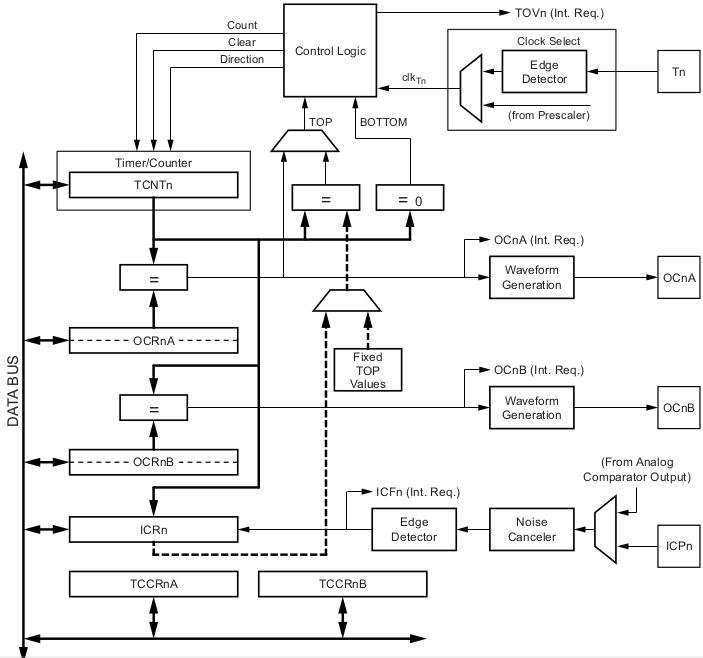
\includegraphics[height=0.6\textheight]{Timer1BlockDiagram.png}
    \end{center}
\end{figure}

\section{Terminologies and Registers}
\begin{minipage}{0.4\textwidth}
    \begin{tabular}{c|p{4.5cm}}
        \textbf{Parameter} & \textbf{Description}\\
        \hline
        BOTTOM & counter reaches 0x0000\\
        MAX & ounter reaches 0xFFFF\\
        TOP & counter reaches highest value (depends on mode of operation can be 0xFF, 0x1FF, 0x3FF, OCR1A, ICR1)
    \end{tabular}
\end{minipage}
\begin{minipage}{0.55\textwidth}
    \begin{tabular}{c|p{5.5cm}}
        \textbf{Register - 16 bit} & \textbf{Name}\\
        \hline
        \regFormat{TCN10} & Timer/Counter1count value\\
        \regFormat{TCCR1A} & Timer/Coutner1 Control Register A\\
        \regFormat{TCCR1B} & Timer/Coutner1 Control Register B\\
        \regFormat{OCBR1A} & Output compare register A\\
        \regFormat{OCBR1B} & Output compare register B\\
        \regFormat{TIFR1} & Timer Interrupt Flag Register\\
        \regFormat{TIMSK1} & Timer interrupt Mask Register\\
        \regFormat{ICR1} & Input Capture Register\\
    \end{tabular}
\end{minipage}

\textbf{Note: } 
\begin{itemize}
    \item The \regFormat{CNT1, OCR1A/B, ICR1} are 16-bit registers that can be accessed by the CPU via the 8-bit data bus.
    \item \textbf{For 16-bit write, the high byte must be written before the low byte.}
    \item \textbf{For 16-bit read, the low byte must be read before the high byte.}
\end{itemize}
\section{Timer/Counter1 Units}

\subsection{Clock Source/Select Unit}
\begin{figure}[H]
    \begin{center}
        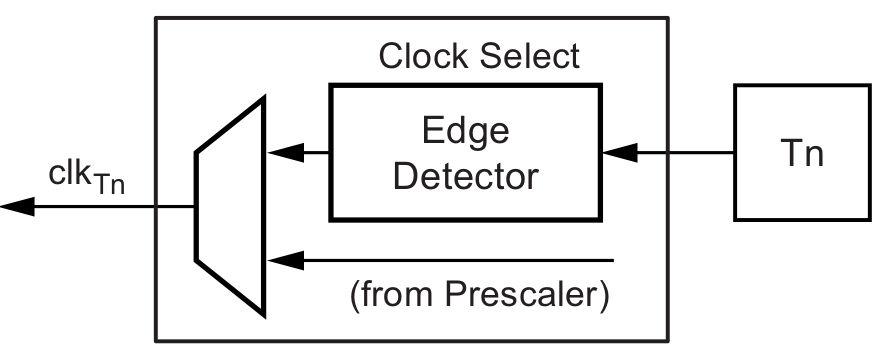
\includegraphics[width=0.5\textwidth]{Timer0ClockSelector.png}
    \end{center}
\end{figure}
\begin{itemize}
    \item The source for the Timer/Counter0 can be external or internal.
    \item External clock source is from \pinFormat{T1} pin.
    \item While Internal Clock source can be clocked via a prescalar.
    \item The output of this unit is the timer clock ($clk_{T1}$).
    \item It uses \bitFormat{CS1[2:0]} bits in \regFormat{TCCR1B} register to select the source.
\end{itemize}


\subsection{Counter Unit}
\begin{minipage}{0.5\textwidth}
    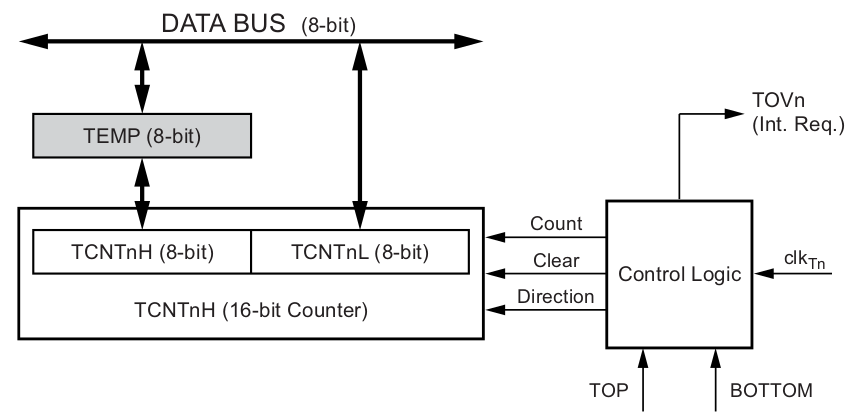
\includegraphics[width=1\textwidth]{Timer1CounterUnit.png}
\end{minipage}
\begin{minipage}{0.45\textwidth}
    \begin{tabular}{c|p{5.5cm}}
        \textbf{Signal} & \textbf{Description}\\
        \hline  
        count & Increment or decrement \regFormat{TCNT1} by 1\\
        direction & Select between increment or decrement\\
        clear & Clears \regFormat{TCNT1} to 0x0000\\
        $clk_{T1}$ & Timer/Coutner1 clock\\
        top & Signalize that \regFormat{TCNT1} has maximum value\\
        bottom & Signalize that \regFormat{TCNT1} has minimum value(0x0000)\\
    \end{tabular}
\end{minipage}
\begin{itemize}
    \item The main part of the 16-bit Timer/Counter is the programmable bi-directional counter.
    \item Counter high (\regFormat{TCNT1H}) containing the upper eight bits of the counter, and counter low (\regFormat{TCNT1L}) containing the lower eight bits.
    \item Depending the mode of operation the counter is cleared, incremented, or decremented at each timer clock ($clk_{T1}$).
    \item Counting sequence is determined by \bitFormat{WGM1[3:0]} bits of \regFormat{TCCR1A} -Timer/Counter1 Control register A and \regFormat{TCCR1B} - Timer/Counter1 Control register B.
    \item The Timer/Counter1 Overflow flag \bitFormat{(TOV1)} is set and can generate interrupt according to the mode.
\end{itemize}

\subsection{Input Capture Unit}
\begin{figure}[H]
    \centering
    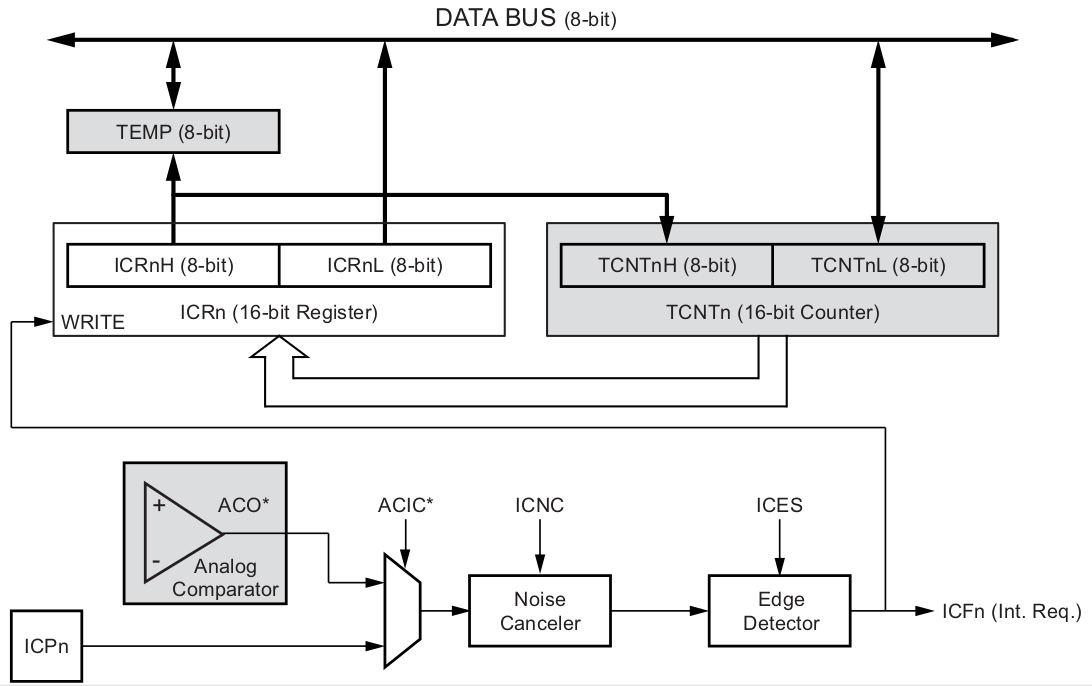
\includegraphics[width=0.75\textwidth]{Timer1InputCapture.png}
\end{figure}
\begin{itemize}
    \item Can capture external events and give them time-stamp indicating time of occurance.
    \item External signal can be from \pinFormat{ICP1} pin or analog-comparator unit.
    \item Usage : calculate frequency, duty-cycle, log of the signal
    \item When a change of the logic level (an event) occurs on the input capture pin (\pinFormat{ICP1}), or on the analog comparator output (\pinFormat{ACO)}, and this change confirms to the setting of the edge detector, a capture will be triggered. 
    \item When a capture is triggered, the 16-bit value of the counter (\regFormat{TCNT1}) is written to the input capture register (\regFormat{ICR1}).
    \item The input capture flag (\bitFormat{ICF1}) is set at the same system clock as the \regFormat{TCNT1} value is copied into \regFormat{ICR1} register. 
    \item If enabled (\bitFormat{ICIE1} = 1), the input capture flag generates an input capture interrupt.
    \item \bitFormat{ICF1} flag is automatically cleared when the interrupt is executed and by writing on to i.
    \item An input capture can be triggered by software by controlling the port of the \pinFormat{ICP1} pin.
\end{itemize}

\subsection{Output Compare Unit}
\begin{figure}[H]
    \begin{center}
        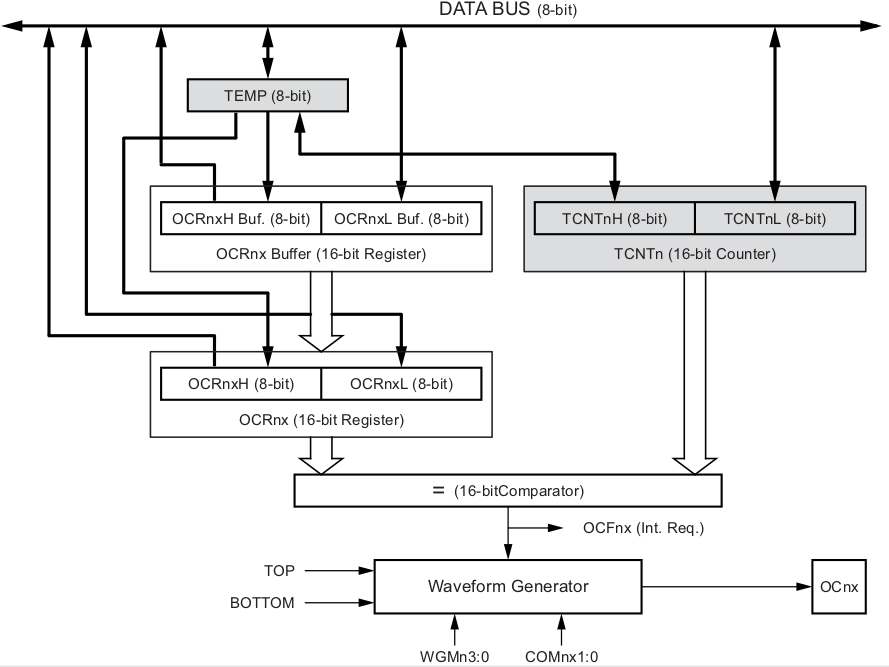
\includegraphics[width=0.6\textwidth]{Timer1OutputCompare.png}
    \end{center}
\end{figure}
\begin{itemize}
    \item 16-bit comparator continuously compares \regFormat{TCNT1} with both \regFormat{OCR1A} and \regFormat{OCR1B}.
    \item When \regFormat{TCNT1} equals \regFormat{OCR1A} or \regFormat{OCR1B}, the comparator signals a match which will set the output compare flag at the next timer clock cycle.
    \item If interrupts are enabled, then output compare interrupt is generated.
    \item The waveform generator uses the match signal to generate an output according to operating mode set by the \bitFormat{WGM1[3:0]} bits and compare output mode \bitFormat{COM0x[1:0]} bits.
\end{itemize}

\subsection{Compare Match Output Unit}
\begin{figure}[H]
    \begin{center}
        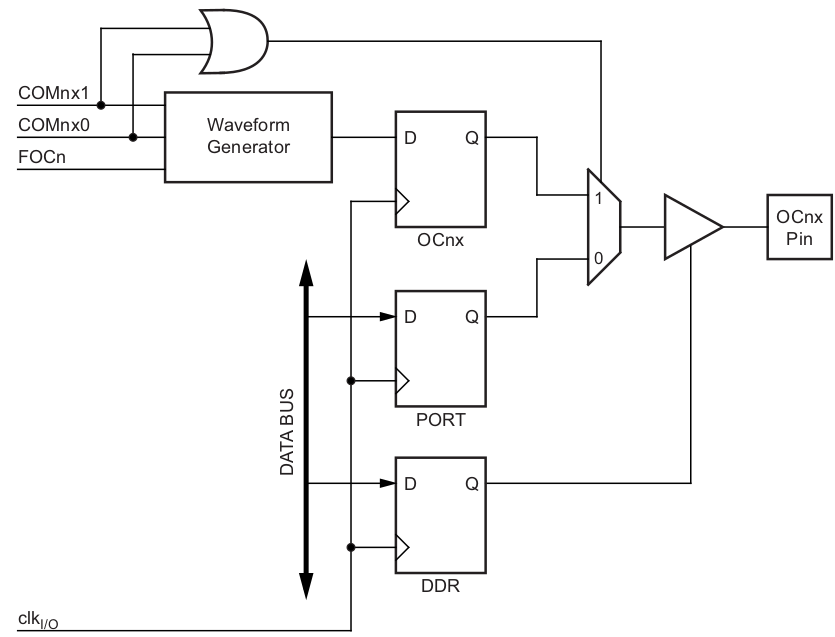
\includegraphics[height=0.3\textheight]{Timer1ComparteMatchOutput.png}
    \end{center}
\end{figure}
\begin{itemize}
    \item This unit is used for changing the state of \pinFormat{OC1A} and \pinFormat{OC1B} pins by configuring the \bitFormat{COM1x[1:0]} bits.
    \item But, general I/O port function is overriiden by DDR reigster.
\end{itemize}


\section{Modes of Operation}
\begin{itemize}
    \item The mode of operation can be defined by combination of waveform generation mode (\bitFormat{WGM1[3:0]}) and compare output mode(\bitFormat{COM1[1:0]}) bits.
    \item The waveform generation mode (\bitFormat{WGM1[3:0]}) bits affect the counting sequence.
    \item For non-PWM mode, \bitFormat{COM1[1:0]} bits control if the output should be set, cleared or toggled at a compare match.
    \item For PWM mode, \bitFormat{COM1[1:0]} bits control if the PWM generated should be inverted or non-inverted.
\end{itemize}



\subsection{Normal Mode - Non-PWM Mode}
\begin{itemize}
    \item \bitFormat{WGM1[3:0]} $-->$ 000.
    \item Counter counts up and no counter clear.
    \item Overruns TOP(0XFFFF) and restarts from BOTTOM(0X0000).
    \item \bitFormat{TOV1} Flag is only set when overrun.
    \item We have to clear \bitFormat{TOV1} flag inorder to have next running.
    \item But, if we use interrupt we don’t need to clear it as interrupt automatically clear the \bitFormat{TOV1} flag.
    \item The input capture unit can be used to capture events at \pinFormat{ICP1} pin or \pinFormat{ACO} pin.
    \item The timing can be seen below.
\end{itemize}

\begin{tikztimingtable}[
    timing/dslope=0.1,
    timing/.style={x=5ex,y=2ex},
    x=5ex,
    timing/rowdist=3ex,
    timing/name/.style={font=\sffamily\scriptsize}
    ]
    \busref{clk\_{T1}}  & 41{c}\\
    \busref{TCNT1} & u{} D{0x0000} D{0x0001};[dotted] 2D{};D{0xFFFE} D{0xFFFF}D{0x0000} D{0x0001};[dotted] 2D{};D{0xFFFE} D{0xFFFF}D{0x0000} D{0x0001};[dotted] 2D{};D{0xFFFE} D{0xFFFF}D{0x0000} D{0x0001}\\
    \busref{TOV1} & l 6{L} H 5{L} H 5{L} H 1{L}\\
\end{tikztimingtable}



\subsection{Clear Timer on Compare Match(CTC) Mode - Non-PWM Mode}
\begin{itemize}
    \item \bitFormat{WGM1[3:0]} $-->$ 0100 or 1100.
    \begin{itemize}
        \item Counter value clears when \regFormat{TCNT1} reaches \regFormat{OCR1A} if \bitFormat{WGM1[3:0]} is 0100.
        \item Counter value clears when \regFormat{TCNT1} reaches \regFormat{ICR1} if \bitFormat{WGM1[3:0]} is 1100.
    \end{itemize}
    \item Interrupt can be generated each time \regFormat{TCNT1} reaches \regFormat{OCR1A} register value by \bitFormat{OCF1A} flag.
    \item Interrupt can be generated each time \regFormat{TCNT1} reaches \regFormat{ICR1} register value by \bitFormat{ICF1} flag.
    \item When \bitFormat{COM1A[1:0]} == 01, the \pinFormat{OC1A} pin output can be set to toggle its match between \regFormat{TCNT1} and \regFormat{OCR1A} or \regFormat{ICR1} register to generate waveform.
    \item The frequency of the waveform its
    \begin{center}
        { \Large $f_{OC1A} = \frac{f_{clkT1}}{2 * N * (1 + OCR1A)}$ }
    \end{center}
    \item Here N is prescalar factor and can be (1, 8, 64, 256, or 1024).
\end{itemize}


\subsubsection{WGM1[3:0] == 0100}
\begin{tikztimingtable}[
    timing/dslope=0.1,
    timing/.style={x=5ex,y=2ex},
    x=5ex,
    timing/rowdist=3ex,
    timing/name/.style={font=\sffamily\scriptsize}
    ]
    \busref{clk\_{T1}}  & 28{1.5c}\\
    \busref{TCNT1} & 0.75U{} 1.5D{0x0000} 1.5D{0x0001};[dotted] 3D{};1.5D{OCR1A - 1} 1.5D{OCR1A}1.5D{0x0000} 1.5D{0x0001};[dotted] 3D{};1.5D{OCR1A - 1} 1.5D{OCR1A} 1.5D{0x0000} 0.75D{0x0001} \\
    \busref{OC1A} & 0.75L 9{L} 1.5H l 7{L} 1.5H l\\
\end{tikztimingtable}
\subsubsection{WGM1[3:0] == 1100}
\begin{tikztimingtable}[
    timing/dslope=0.1,
    timing/.style={x=5ex,y=2ex},
    x=5ex,
    timing/rowdist=3ex,
    timing/name/.style={font=\sffamily\scriptsize}
    ]
    \busref{clk\_{T1}}  & 28{1.5c}\\
    \busref{TCNT1} & 0.75U{} 1.5D{0x0000} 1.5D{0x0001};[dotted] 3D{};1.5D{ICR1 - 1} 1.5D{ICR1}1.5D{0x0000} 1.5D{0x0001};[dotted] 3D{};1.5D{ICR1 - 1} 1.5D{ICR1} 1.5D{0x0000} 0.75D{0x0001} \\
    \busref{OC1A} & 0.75L 9{L} 1.5H l 7{L} 1.5H l\\
\end{tikztimingtable}

\subsection{Fast PWM Mode}
\begin{itemize}
    \item \bitFormat{WGM1[3:0]} $-->$ 0101 or 0110 or 0111 or 1110 or 1111.
    \item Power Regulation, Rectification, DAC applications.
    \item Single slope operations causing high frequency PWM waveform.
    \item Counter starts from BOTTOM to TOP and then restarts from BOTTOM.
    \item TOP is defined by
    \begin{itemize}
        \item TOP == 0x00FF if \bitFormat{WGM1[3:0]} $-->$ 0101
        \item TOP == 0x01FF if \bitFormat{WGM1[3:0]} $-->$ 0110
        \item TOP == 0x03FF if \bitFormat{WGM1[3:0]} $-->$ 0111
        \item TOP ==   \regFormat{ICR1} if \bitFormat{WGM1[3:0]} $-->$ 1110
        \item TOP ==  \regFormat{OCR1A} if \bitFormat{WGM1[3:0]} $-->$ 1111
    \end{itemize}
    \item  When \bitFormat{COM1A[1:0]} == 01, the \pinFormat{OC1A} pin output can be set to toggle its match between \regFormat{TCNT1} and TOP to generate waveform.
    \begin{itemize}
        \item The above is possible only when \bitFormat{WGM12} bit is set.
        \item And only on \pinFormat{OC1A} pin and not on \pinFormat{OC1B} pin.
    \end{itemize}
    \item In Inverting Compare Mode \bitFormat{COM1A[1:0]} == 10 , the \pinFormat{OC1A} or \pinFormat{OC1B} pins is made 1 on compare match between \regFormat{TCNT1} and TOP and made 0 on reaching BOTTOM.
    \item In Non-Inverting Compare Mode \bitFormat{COM1A[1:0]} == 11 , the \pinFormat{OC1A} or \pinFormat{OC1B} pins is made 0 on compare match between \regFormat{TCNT1} and TOP and 1 made  on reaching BOTTOM.
    \item The Timer/Counter overflow flag (\bitFormat{TOV1}) is set each time the counter reaches TOP.
    \item The PWM frequency is given by 
    \begin{center}
        { \Large $f_{OC1xPWM} = \frac{f_{clkT1}}{N * (1+ TOP)}$ }
    \end{center}
\end{itemize}

\subsubsection{WGM1[3:0] == 0101}
\begin{tikztimingtable}[
    timing/dslope=0.1,
    timing/.style={x=5ex,y=2ex},
    x=5ex,
    timing/rowdist=3ex,
    timing/name/.style={font=\sffamily\scriptsize}
    ]
    \busref{clk\_{T0}}  & 41{1c} c\\
    \busref{TCNT1} & 0.5U{} D{0x0000} 1D{0x0001};[dotted] 1.5D{};1D{0x00FE} 1D{0x00FF}1D{0x0000} 1D{0x0001};[dotted] 1D{};1D{0x00FE} 1D{0x00FF} 1D{0x0000} 1D{0x0001} [dotted] 1D{};1D{0x00FE} 1D{0x00FF} 1D{0x0000} 1D{0x0001};[dotted] 1D{};1D{0x00FE} 1D{0x00FF};\\
    \busref{TOV1} & 6{L} H 4{L} H 4{L} H 4{L} \\
\end{tikztimingtable}

\subsubsection{WGM1[3:0] == 0110}
\begin{tikztimingtable}[
    timing/dslope=0.1,
    timing/.style={x=5ex,y=2ex},
    x=5ex,
    timing/rowdist=3ex,
    timing/name/.style={font=\sffamily\scriptsize}
    ]
    \busref{clk\_{T0}}  & 41{1c} c\\
    \busref{TCNT1} & 0.5U{} D{0x0000} 1D{0x0001};[dotted] 1.5D{};1D{0x01FE} 1D{0x01FF}1D{0x0000} 1D{0x0001};[dotted] 1D{};1D{0x01FE} 1D{0x01FF} 1D{0x0000} 1D{0x0001} [dotted] 1D{};1D{0x01FE} 1D{0x01FF} 1D{0x0000} 1D{0x0001};[dotted] 1D{};1D{0x01FE} 1D{0x01FF};\\
    \busref{TOV1} & 6{L} H 4{L} H 4{L} H 4{L} \\
\end{tikztimingtable}
\subsubsection{WGM1[3:0] == 0111}
\begin{tikztimingtable}[
    timing/dslope=0.1,
    timing/.style={x=5ex,y=2ex},
    x=5ex,
    timing/rowdist=3ex,
    timing/name/.style={font=\sffamily\scriptsize}
    ]
    \busref{clk\_{T0}}  & 41{1c} c\\
    \busref{TCNT1} & 0.5U{} D{0x0000} 1D{0x0001};[dotted] 1.5D{};1D{0x03FE} 1D{0x03FF}1D{0x0000} 1D{0x0001};[dotted] 1D{};1D{0x03FE} 1D{0x03FF} 1D{0x0000} 1D{0x0001} [dotted] 1D{};1D{0x03FE} 1D{0x03FF} 1D{0x0000} 1D{0x0001};[dotted] 1D{};1D{0x03FE} 1D{0x03FF};\\
    \busref{TOV1} & 6{L} H 4{L} H 4{L} H 4{L} \\
\end{tikztimingtable}

\subsubsection{WGM1[3:0] == 1110}
\begin{tikztimingtable}[
    timing/dslope=0.1,
    timing/.style={x=5ex,y=2ex},
    x=5ex,
    timing/rowdist=3ex,
    timing/name/.style={font=\sffamily\scriptsize}
    ]
    \busref{clk\_{T0}}  & 41{1c} c\\
    \busref{TCNT1} & 0.5U{} D{0x0000} 1D{0x001};[dotted] 1.5D{};1D{\tiny ICR1 -1} 1D{\tiny ICR1}1D{0x0000} 1D{0x0001};[dotted] 1D{};1D{\tiny ICR1 -1} 1D{\tiny ICR1} 1D{0x0000} 1D{0x0001} [dotted] 1D{};1D{\tiny ICR1 -1} 1D{\tiny ICR1} 1D{0x0000} 1D{0x0001};[dotted] 1D{};1D{\tiny ICR1 -1} 1D{\tiny ICR1};\\
    \busref{TOV1} & 6{L} H 4{L} H 4{L} H 4{L} \\
\end{tikztimingtable}

\subsubsection{WGM1[3:0] == 1111}
\begin{tikztimingtable}[
    timing/dslope=0.1,
    timing/.style={x=5ex,y=2ex},
    x=5ex,
    timing/rowdist=3ex,
    timing/name/.style={font=\sffamily\scriptsize}
    ]
    \busref{clk\_{T0}}  & 41{1c} c\\
    \busref{TCNT1} & 0.5U{} D{0x0000} 1D{0x001};[dotted] 1.5D{};1D{\tiny OCR1A -1} 1D{\tiny OCR1A}1D{0x0000} 1D{0x0001};[dotted] 1D{};1D{\tiny OCR1A -1} 1D{\tiny OCR1A} 1D{0x0000} 1D{0x0001} [dotted] 1D{};1D{\tiny OCR1A -1} 1D{\tiny OCR1A} 1D{0x0000} 1D{0x0001};[dotted] 1D{};1D{\tiny OCR1A -1} 1D{\tiny OCR1A};\\
    \busref{TOV1} & 6{L} H 4{L} H 4{L} H 4{L} \\
\end{tikztimingtable}

\subsection{Phase Correct PWM Mode}
\begin{itemize}
    \item \bitFormat{WGM1[3:0]} $-->$ 0001 or 0010 or 0011 or 1010 or 1011.    
    \item High resolution phase correct PWM.
    \item Motor control due to symmetric features
    \item Dual slope operations causing ower frequency PWM waveform.
    \item Counter starts from BOTTOM to TOP and then from TOP to BOTTOM.
    \item TOP is defined by
    \begin{itemize}
        \item TOP == 0x00FF if \bitFormat{WGM1[3:0]} $-->$ 0001
        \item TOP == 0x01FF if \bitFormat{WGM1[3:0]} $-->$ 0010
        \item TOP == 0x03FF if \bitFormat{WGM1[3:0]} $-->$ 0011
        \item TOP ==   \regFormat{ICR1} if \bitFormat{WGM1[3:0]} $-->$ 1010
        \item TOP ==  \regFormat{OCR1A} if \bitFormat{WGM1[3:0]} $-->$ 1011
    \end{itemize}
    \item  When \bitFormat{COM1A[1:0]} == 01, the \pinFormat{OC1A} pin output can be set to toggle its match between \regFormat{TCNT1} and TOP to generate waveform.
    \begin{itemize}
        \item The above is possible only when \bitFormat{WGM12} bit is set.
        \item And only on \pinFormat{OC1A} pin and not on \pinFormat{OC1B} pin.
    \end{itemize}
    \item In Inverting Compare Mode \bitFormat{COM1A[1:0]} == 10 , the \pinFormat{OC1A} or \pinFormat{OC1B} pins is made 1 on compare match between \regFormat{TCNT1} and TOP and made 0 on reaching BOTTOM.
    \item In Non-Inverting Compare Mode \bitFormat{COM1A[1:0]} == 11 , the \pinFormat{OC1A} or \pinFormat{OC1B} pins is made 0 on compare match between \regFormat{TCNT1} and TOP and 1 made  on reaching BOTTOM.
    \item The Timer/Counter overflow flag (\bitFormat{TOV1}) is set each time the counter reaches BOTTOM..
    \item The PWM frequency is given by 
    \begin{center}
        { \Large $f_{OC1xPWM} = \frac{f_{clkT1}}{2 * N * TOP}$ }
    \end{center}
\end{itemize}


\subsubsection{WGM1[3:0] == 0001}
\begin{tikztimingtable}[
    timing/dslope=0.1,
    timing/.style={x=5ex,y=2ex},
    x=5ex,
    timing/rowdist=3ex,
    timing/name/.style={font=\sffamily\scriptsize}
    ]
    \busref{clk\_{T1}}  & 41{1c} c\\
    \busref{TCNT1} & 0.5U{} D{0x0000} 1D{0x0001};[dotted] 1.5D{};1D{0x00FE} 1D{0x00FF}1D{0x0000} 1D{0x0001};[dotted] 1D{};1D{0x00FE} 1D{0x00FF} 1D{0x0000} 1D{0x0001} [dotted] 1D{};1D{0x00FE} 1D{0x00FF} 1D{0x0000} 1D{0x0001};[dotted] 1D{};1D{0x00FE} 1D{0x00FF};\\
    \busref{TOV1} & 6{L} H 4{L} H 4{L} H 4{L} \\
\end{tikztimingtable}


\subsubsection{WGM1[3:0] == 0010}
\begin{tikztimingtable}[
    timing/dslope=0.1,
    timing/.style={x=5ex,y=2ex},
    x=5ex,
    timing/rowdist=3ex,
    timing/name/.style={font=\sffamily\scriptsize}
    ]
    \busref{clk\_{T1}}  & 41{1c} c\\
    \busref{TCNT1} & 0.5U{} D{0x0000} 1D{0x0001};[dotted] 1.5D{};1D{0x01FE} 1D{0x01FF}1D{0x0000} 1D{0x0001};[dotted] 1D{};1D{0x01FE} 1D{0x01FF} 1D{0x0000} 1D{0x0001} [dotted] 1D{};1D{0x01FE} 1D{0x01FF} 1D{0x0000} 1D{0x0001};[dotted] 1D{};1D{0x01FE} 1D{0x01FF};\\
    \busref{TOV1} & 6{L} H 4{L} H 4{L} H 4{L} \\
\end{tikztimingtable}

\subsubsection{WGM1[3:0] == 0011}
\begin{tikztimingtable}[
    timing/dslope=0.1,
    timing/.style={x=5ex,y=2ex},
    x=5ex,
    timing/rowdist=3ex,
    timing/name/.style={font=\sffamily\scriptsize}
    ]
    \busref{clk\_{T1}}  & 41{1c} c\\
    \busref{TCNT1} & 0.5U{} D{0x0000} 1D{0x0001};[dotted] 1.5D{};1D{0x03FE} 1D{0x03FF}1D{0x0000} 1D{0x0001};[dotted] 1D{};1D{0x03FE} 1D{0x03FF} 1D{0x0000} 1D{0x0001} [dotted] 1D{};1D{0x03FE} 1D{0x03FF} 1D{0x0000} 1D{0x0001};[dotted] 1D{};1D{0x03FE} 1D{0x03FF};\\
    \busref{TOV1} & 6{L} H 4{L} H 4{L} H 4{L} \\
\end{tikztimingtable}

\subsubsection{WGM[2:0] == 1010}
\begin{tikztimingtable}[
    timing/dslope=0.1,
    timing/.style={x=5ex,y=2ex},
    x=5ex,
    timing/rowdist=3ex,
    timing/name/.style={font=\sffamily\scriptsize}
    ]
    \busref{clk\_{T1}}  & 41{1c}\\
    \busref{TCNT1} & 0.5U{} D{0x0000} 1D{0x0001};[dotted] 1.5D{};1D{\tiny OCR1A - 1} 1D{\tiny OCR1A}1D{\tiny OCR01-1} 1D{\tiny OCR1A-2};[dotted] 1D{};1D{0x0001} 1D{0x0000} 1D{0x0001}[dotted] 1D{};1D{\tiny OCR1A-1} 1D{\tiny OCR1A} 1D{\tiny OCR1A-1} 1D{\tiny OCR1A-2};[dotted] 1D{};1D{0x0001} 1D{0x0000} 1d{0x0001};\\
    \busref{TOV1} & l H l 8{L} H 8{L} H l\\
\end{tikztimingtable}

\subsubsection{WGM[2:0] == 1011}
\begin{tikztimingtable}[
    timing/dslope=0.1,
    timing/.style={x=5ex,y=2ex},
    x=5ex,
    timing/rowdist=3ex,
    timing/name/.style={font=\sffamily\scriptsize}
    ]
    \busref{clk\_{T1}}  & 41{1c}\\
    \busref{TCNT1} & 0.5U{} D{0x0000} 1D{0x0001};[dotted] 1.5D{};1D{\tiny ICR1- 1} 1D{\tiny ICR1}1D{\tiny ICR1-1} 1D{\tiny ICR1-2};[dotted] 1D{};1D{0x0001} 1D{0x0000} 1D{0x0001}[dotted] 1D{};1D{\tiny ICR1-1} 1D{\tiny ICR1} 1D{\tiny ICR1-1} 1D{\tiny ICR1-2};[dotted] 1D{};1D{0x0001} 1D{0x0000} 1d{0x0001};\\
    \busref{TOV1} & l H l 8{L} H 8{L} H l\\
\end{tikztimingtable}

\subsection{Phase and Frequency Corrected PWM Mode}
\begin{itemize}
    \item \bitFormat{WGM1[3:0]} $-->$ 1000 or 1001.
    \item High resolution and Phase correctd PWM.
    \item Dual-Slope.
    \item Counter counts from BOTTOM to TOP and then from TOP to BOTTOM.
    \begin{itemize}
        \item TOP == \regFormat{OCR1A} if \bitFormat{WGM1[3:0]} $-->$ 1001
        \item TOP == \regFormat{ICR1} if \bitFormat{WGM1[3:0]} $-->$ 1000
    \end{itemize}
    \item In Inverting Compare Mode \bitFormat{COM1x[1:0]} == 10 the \pinFormat{OC0x} pins is made 1 on compare match between \regFormat{TCNT1} and TOP when upcounting and made 0 on compare match between \regFormat{TCNT1} and TOP when downcounting.
    \item In Non-Inverting Compare Mode \bitFormat{COM1x[1:0]} == 11, the \pinFormat{OC0x} pins is made 0 on compare match between \regFormat{TCNT1} and TOP when upcounting AND made 1 on compare match between \regFormat{TCNT1} and TOP when downcounting.
    \item The Timer/Counter overflow flag (\bitFormat{TOV1}) is set each time the counter reaches BOTTOM.
    \item The interrupt flag can be used to generate an interrupt each time the counter reaches the BOTTOM value.
    \item The PWM frequency is given by 
    \begin{center}
        { \Large $f_{OC1xPWM} = \frac{f_{clkT1}}{2 * N * TOP}$ }
    \end{center}
\end{itemize}
\newpage

\section{Register Description}
\subsubsection*{TCCR1A – Timer/Counter 1 Control Register A}
\vspace*{0.5cm}
\begin{bytefield}[bitformatting={\large\bfseries},
    endianness=big,bitwidth=0.125\linewidth]{8}
    \bitheader[lsb=0]{0-7} \\
    \bitbox{1}{\small COM1A1}
    \bitbox{1}{\small COM1A0}
    \bitbox{1}{\small COM1B1}
    \bitbox{1}{\small COM1B0}
    \bitbox{1}{\small -}
    \bitbox{1}{\small -}
    \bitbox{1}{\small WGM11}
    \bitbox{1}{\small WGM10}\\
\end{bytefield}

\begin{table}[H]
    \begin{center}
        \begin{tabular}{c|p{4.1cm}|p{4.5cm}|p{4.9cm}}
            \bitFormat{COM1x[1:0]} & \textbf{Non-PWM modes} & \textbf{Fast PWM} & \textbf{Phase Corrected PWM \& Phase and Frequency Corrected PWM}\\
            \hline
            00 & No output @ \pinFormat{PB1 - OC1A} or \pinFormat{PB2 - OC1B} pin &   No output @ \pinFormat{PB1 - OC1A} or \pinFormat{PB2 - OC1B} pin & No output @ \pinFormat{PB1 - OC1A} or \pinFormat{PB2 - OC1B} pin \\
            \hline
            01 &  Toggle \pinFormat{PB1 - OC1A} or \pinFormat{PB2 - OC1B} pin on compare Match. & When \bitFormat{WGM[3:0]} == 1110 or 1111, Toggle \pinFormat{OC1A} pin on compare match & When \bitFormat{WGM[3:0]} == 1110 or 1111, Toggle \pinFormat{OC1A} pin on comapre match.\\
            \hline
            10 & Clear \pinFormat{PB1 - OC1A} or \pinFormat{PB2 - OC1B} pin on compare Match. & Clear \pinFormat{PB1 - OC1A} or \pinFormat{PB2 - OC1B} on compare match and  set \pinFormat{PB1 - OC1A} or \pinFormat{PB2 - OC1B} at BOTTOM & Clear \pinFormat{PD5 - OC0B} on compare match when up-counting and set \pinFormat{PB1 - OC1A} or \pinFormat{PB2 - OC1B} on compare match when down-counting.\\
            \hline
            11 & Set \pinFormat{PB1 - OC1A} or \pinFormat{PB2 - OC1B} pin on compare Match. & Set \pinFormat{PB1 - OC1A} or \pinFormat{PB2 - OC1B} on compare match and clear \pinFormat{PB1 - OC1A} or \pinFormat{PB2 - OC1B} at BOTTOM & Set \pinFormat{PD5 - OC0B} on compare match when up-counting and clear \pinFormat{PB1 - OC1A} or \pinFormat{PB2 - OC1B} on compare match when down-counting.\\
        \end{tabular}
    \end{center}
\end{table}


\begin{table}[H]
    \begin{center}
        \begin{tabular}{c|c|c|c}
            \bitFormat{WGM1[3:0]} & \textbf{Mode of operation} & \textbf{TOP} & \textbf{TOV1 Flag set on}\\
            \hline
            0000 & Normal & 0xFFFF & MAX\\
            0001 & PWM Phase corrected – 8bit & 0x00FF & BOTTOM\\
            0010 & PWM Phase corrected – 9bit & 0x01FF & BOTTOM\\
            0011 & PWM Phase corrected – 10bit & 0x03FF & BOTTOM\\
            0100 & CTC & OCR1A & MAX\\
            0101 & Fast PWM – 8bit & 0x00FF & TOP\\
            0110 & Fast PWM – 9bit & 0x01FF & TOP\\
            0111 & Fast PWM – 10bit & 0x03FF & TOP\\
            1000 & PWM, phase and frequency corrected & ICR1 & BOTTOM\\
            1001 & PWM, phase and frequency corrected & OCR1A & BOTTOM\\
            1010 & PWM, phase corrected & ICR1 & BOTTOM\\
            1011 & PWM, phase corrected & OCR1A & BOTTOM\\
            1100 & CTC & ICR1 & MAX\\
            1110 & Fast PWM & ICR1 & TOP\\
            1111 & Fast PWM & OCR1A & TOP\\
        \end{tabular}
    \end{center}
\end{table}

\subsubsection*{TCCR1B – Timer/Counter1 Control Register B}
\vspace*{0.5cm}
\begin{bytefield}[bitformatting={\large\bfseries},
    endianness=big,bitwidth=0.125\linewidth]{8}
    \bitheader[lsb=0]{0-7} \\
    \bitbox{1}{\small ICNC1}
    \bitbox{1}{\small ICES1}
    \bitbox{1}{\small -}
    \bitbox{1}{\small WGM13}
    \bitbox{1}{\small WGM12}
    \bitbox{1}{\small CS12}
    \bitbox{1}{\small CS11}
    \bitbox{1}{\small CS10}\\
\end{bytefield}
\begin{itemize}
    \item \bitFormat{ICNC1 - Input Capture Noise Canceler} - activates the input capture noise canceler.
    \item \bitFormat{ICES1 - Input Capture Edge Select} - selects which edge on the input capture pin (\pinFormat{ICP1}) that is used to trigger a capture event. [1 - Rising edge; 0 - falling edge;]
\end{itemize}

\begin{table}[H]
    \begin{center}
        \begin{tabular}{c|c}
            \bitFormat{CS1[2:0]} & \textbf{Description(Prescalar)}\\
            \hline
            000 & No clock source(Timer/Counter Stopped)\\
            001 & $clk_{I/O}$ – no prescaling\\
            010 & $\frac{clk_{I/O}}{8}$\\
            011 & $\frac{clk_{I/O}}{64}$\\\
            100 & $\frac{clk_{I/O}}{256}$\\\
            101 & $\frac{clk_{I/O}}{1024}$\\\
            110 & External clock source on \pinFormat{T1} pin. Clock on falling edge.\\
            111 & External clock source on \pinFormat{T1} pin. Clock on rising edge.\\
        \end{tabular}
    \end{center}
\end{table}

\subsubsection*{TCNT1H – Timer/Counter1 Counter Higher Byte}
\vspace*{0.5cm}
\begin{bytefield}[bitformatting={\large\bfseries},
    endianness=big,bitwidth=0.125\linewidth]{8}
    \bitheader[lsb=0]{0-7} \\
    \bitbox{8}{TCNT1[15:8]}\\
\end{bytefield}
\subsubsection*{TCNT1L – Timer/Counter1 Counter Lower Byte}
\vspace*{0.5cm}
\begin{bytefield}[bitformatting={\large\bfseries},
    endianness=big,bitwidth=0.125\linewidth]{8}
    \bitheader[lsb=0]{0-7} \\
    \bitbox{8}{TCNT1[7:0]}\\
\end{bytefield}

\subsubsection*{OCR1AH – Output Compare Register 1 A Higher Byte}
\vspace*{0.5cm}
\begin{bytefield}[bitformatting={\large\bfseries},
    endianness=big,bitwidth=0.125\linewidth]{8}
    \bitheader[lsb=0]{0-7} \\
    \bitbox{8}{OCR1A[15:8]}\\
\end{bytefield}
\subsubsection*{OCR1AL – Output Compare Register 1 A Lower Byte}
\vspace*{0.5cm}
\begin{bytefield}[bitformatting={\large\bfseries},
    endianness=big,bitwidth=0.125\linewidth]{8}
    \bitheader[lsb=0]{0-7} \\
    \bitbox{8}{OCR1A[7:0]}\\
\end{bytefield}

\subsubsection*{OCR1BH – Output Compare Register 1 B Higher Byte}
\vspace*{0.5cm}
\begin{bytefield}[bitformatting={\large\bfseries},
    endianness=big,bitwidth=0.125\linewidth]{8}
    \bitheader[lsb=0]{0-7} \\
    \bitbox{8}{OCR1B[15:8]}\\
\end{bytefield}
\subsubsection*{OCR1BL – Output Compare Register 1 B Lower Byte}
\vspace*{0.5cm}
\begin{bytefield}[bitformatting={\large\bfseries},
    endianness=big,bitwidth=0.125\linewidth]{8}
    \bitheader[lsb=0]{0-7} \\
    \bitbox{8}{OCR1B[7:0]}\\
\end{bytefield}

\subsubsection*{ICR1H – Input Capture Register 1 Higher Byte}
\vspace*{0.5cm}
\begin{bytefield}[bitformatting={\large\bfseries},
    endianness=big,bitwidth=0.125\linewidth]{8}
    \bitheader[lsb=0]{0-7} \\
    \bitbox{8}{ICR1[15:8]}\\
\end{bytefield}
\subsubsection*{ICR1L – Input Capture Register 1 Lower Byte}
\vspace*{0.5cm}
\begin{bytefield}[bitformatting={\large\bfseries},
    endianness=big,bitwidth=0.125\linewidth]{8}
    \bitheader[lsb=0]{0-7} \\
    \bitbox{8}{ICR1[7:0]}\\
\end{bytefield}

\subsubsection*{TIMSK1 – Timer/Counter 1 Interrupt Mask Register}
\vspace*{0.5cm}
\begin{bytefield}[bitformatting={\large\bfseries},
    endianness=big,bitwidth=0.125\linewidth]{8}
    \bitheader[lsb=0]{0-7} \\
    \bitbox{1}{\small -}
    \bitbox{1}{\small -}
    \bitbox{1}{\small ICIE1}
    \bitbox{1}{\small -}
    \bitbox{1}{\small -}
    \bitbox{1}{\small OCIE1B}
    \bitbox{1}{\small OCIE1A}
    \bitbox{1}{\small TOIE1}\\
\end{bytefield}

\quad Enable interrupts for compare match between \regFormat{TCNT1} and \regFormat{OCR1A} or \regFormat{TCNT1} and \regFormat{OCR1B} or overflow in \regFormat{TCNT1} or Input capture interrupt enable.


\subsubsection*{TIFR1 – Timer/Counter 1 Interrupt Flag Register}
\vspace*{0.5cm}
\begin{bytefield}[bitformatting={\large\bfseries},
    endianness=big,bitwidth=0.125\linewidth]{8}
    \bitheader[lsb=0]{0-7} \\
    \bitbox{1}{\small -}
    \bitbox{1}{\small -}
    \bitbox{1}{\small ICF1}
    \bitbox{1}{\small -}
    \bitbox{1}{\small -}
    \bitbox{1}{\small OCIE1B}
    \bitbox{1}{\small OCIE1A}
    \bitbox{1}{\small TOIE1}\\
\end{bytefield}

\quad Flag registers for interrupts on compare match between \regFormat{TCNT0} and \regFormat{OCR0A} or \regFormat{TCNT0} and \regFormat{OCR0B} or overflow in \regFormat{TCNT1} or capture event occurs on the \pinFormat{ICP1} pin .


\section{Configuring the Timer/Counter}
\subsection{Normal Mode}
\subsubsection{As Timer}
\begin{center}
    $ON\_TIME = \frac{max\_count}{\frac{F\_CPU}{PRESCALAR}}$
\end{center}
\begin{itemize}
    \item Depending on PRESCALR value, we get different ON\_TIME.
    \item First, \bitFormat{WGM1[3:0]} bits are configured as 0000 for Normal Mode in \regFormat{TCCR1A} and \regFormat{TCCR1B} registers.
    \item Next, \bitFormat{COM1A[1:0]} and/or \bitFormat{COM1A[1:0]} bits are configured to make outputs \pinFormat{OC1A} and/or \pinFormat{OC1B} pins to do nothing, set, clear or toggle in \regFormat{TCCR1A} register.
    \item Next, Interrupt is Enabled by \bitFormat{TOIE1} (overflow enable) in \regFormat{TIMSK1} reigster.
    \item Finally, Timer is started by setting prescalar in \bitFormat{CS1[2:0]} bits as needed prescalar of \regFormat{TCR1B} reigster.
    \item Global Interrupt is enabled.
    \item A interrupt Service Routine for Timer1 overflow is Written.
    \item No need to clear the overflow flag as it is done by hardware.
    \item The timing when both pins \pinFormat{OC1A} and \pinFormat{OC1B} are made to toggle.
\end{itemize}

\begin{tikztimingtable}[
    timing/dslope=0.1,
    timing/.style={x=5ex,y=2ex},
    x=5ex,
    timing/rowdist=3ex,
    timing/name/.style={font=\sffamily\scriptsize}
    ]
    \busref{clk\_{T1}}  & 41{c}\\
    \busref{TCNT1} & u{} D{0x0000} D{0x0001};[dotted] 2D{};D{0xFFFE} D{0xFFFF}D{0x0000} D{0x0001};[dotted] 2D{};D{0xFFFE} D{0xFF}D{0x0000} D{0x0001};[dotted] 2D{};D{0xFFFE} D{0xFFFF}D{0x0000} D{0x0001}\\
    \busref{TOV1} & u h h 5{L} H 5{L} H 5{L} H 1{L}\\
    \busref{OC1A} & l H 5{H} 6{L} 6{H} 2{L}\\
    \busref{OC1B} & h L 5{L} 6{H} 6{L} 2{H}\\
\end{tikztimingtable}
\begin{itemize}
    \item The code can be seen below,
\end{itemize}
\begin{minted}[breaklines, bgcolor=lightgray]{c}
// MOde of operation to Normal Mode -- WGM1[3:0] === 0000
// WGM1[3](bit4) from TCCR1B, WGM1[2](bit3) from TCCR1B, WGM1[1](bit1)  from TCC1RA, WGM1[0](bit0)  from TCCR1A	
TCCR1A = TCCR1A & ~(1<<WGM10);
TCCR1A = TCCR1A & ~(1<<WGM11);
TCCR1B = TCCR1B & ~(1<<WGM12);
TCCR1B = TCCR1B & ~(1<<WGM13);

/* What to do when timer reaches the MAX(0xFFFF) value */
// toggle OC1A on each time when reaches the MAX(0xFFFF)
// which is reflected in PB1
// Output OC1A to toglle when reaches MAX -- COM1A[1:0] === 01
// COM1A[1](bit7) from TCCR1A, COM1A[0](bit6) from TCCR1A
TCCR1A = TCCR1A & ~(1<<COM1A1);
TCCR1A = TCCR1A | (1<<COM1A0);

// toggle OC1B on each time when reaches the MAX(0xFFFF)
// which is reflected in PB2
// Output OC1B to toglle when reaches MAX -- COM1B[:0] === 01
// COM1B[1](bit5) from TCCR1A, COM1B[0](bit4) from TCCR1A
TCCR1A = TCCR1A & ~(1<<COM1B1);
TCCR1A = TCCR1A | (1<<COM1B0);


//Enable Interrupt of OVERFLOW flag so that interrupt can be generated
TIMSK1 = TIMSK1 | (1<<TOV1);

// start timer by setting the clock prescalar
// SAME AS from I/O clock
// same-- CS1[2:0] === 001
// CS1[2](bit2) from TCCR1B,CS1[1](bit1) from TCCR1B,CS1[0](bit0) from TCCR1B
TCCR1B = TCCR1B | (1<<CS10);
TCCR1B = TCCR1B & ~(1<<CS11);
TCCR1B = TCCR1B & ~(1<<CS12);

// enabling global interrupt

sei();
// SO ON TIME = max_count / (F_CPU / PRESCALAR)
// ON TIME = 0xFFFF / (16000000/1) = 4.096ms
// since symmetric as toggling OFF TIME = 4.096ms
// hence, we get a square wave of fequency 1 / 8.192ms = 122.07Hz
\end{minted}


\subsubsection{As Counter}
\begin{itemize}
    \item Every rising/falling edge the count increases.
    \item So to reach 0xFFFF count, it would take a time of $\frac{0xFFFF}{frequency @ \pinFormat{T1} pin}$.
    \item First, \bitFormat{WGM1[3:0]} bits are configured as 0000 for Normal Mode in \regFormat{TCCR1A} and \regFormat{TCCR1B} registers.
    \item Finally, Counter is started by configuring \bitFormat{CS1[2:0]} bits to 110 or 111 for external falling or rising edge on \pinFormat{T1 - PD5}.
    \item The code when \pinFormat{T1} pin is used as counter @ falling edge.
\end{itemize}
\begin{minted}[breaklines,bgcolor=lightgray]{c}
// MOde of operation to Normal Mode -- WGM1[3:0] === 0000
// WGM1[3](bit4) from TCCR1B, WGM1[2](bit3) from TCCR1B, WGM1[1](bit1)  from TCC1RA, WGM1[0](bit0)  from TCCR1A	
TCCR1A = TCCR1A & ~(1<<WGM10);
TCCR1A = TCCR1A & ~(1<<WGM11);
TCCR1B = TCCR1B & ~(1<<WGM12);
TCCR1B = TCCR1B & ~(1<<WGM13);
    
/* to count external event -we must connect source to T1 (PD5) */
// THE CLK IS CLOCKED FROM external source
// Falling edge of T1(PD5) -- CS1[2:0] === 110
// CS1[2](bit2) from TCCR1B,CS1[1](bit1) from TCCR1B,CS1[0](bit0) from TCCR1B
TCCR1B = TCCR1B & ~(1<<CS10);
TCCR1B = TCCR1B | (1<<CS11);
TCCR1B = TCCR1B | (1<<CS12);
\end{minted}

\subsubsection{As Input Capture}
\begin{itemize}
    \item Capture the value of \regFormat{TCNT1} into \regFormat{ICR1} register when there is rising or falling edge.
    \item First, \bitFormat{WGM1[3:0]} bits are configured as 0000 for Normal Mode in \regFormat{TCCR1A} and \regFormat{TCCR1B} registers.
    \item Next, the falling or rising edge for the \pinFormat{ICP1} pin is selected by \bitFormat{ICES1} bit in \regFormat{TCCR1B}.
    \item The interrupts for input capture is enabled by setting the \bitFormat{ICIE1} bit in \regFormat{TIMSK1}.
    \item A interrupt service routing is written.
    \item Finally, Timer is started by setting prescalar in \bitFormat{CS1[2:0]} bits as needed prescalar of \regFormat{TCR1B} reigster.
    \item The code when \pinFormat{ICP1 - PB0} pin is used as capture @ rising edge.
\end{itemize}
\begin{minted}[breaklines,bgcolor=lightgray]{c}
// MOde of operation to Normal Mode -- WGM1[3:0] === 0000
// WGM1[3](bit4) from TCCR1B, WGM1[2](bit3) from TCCR1B, WGM1[1](bit1)  from TCC1RA, WGM1[0](bit0)  from TCCR1A	
TCCR1A = TCCR1A & ~(1<<WGM10);
TCCR1A = TCCR1A & ~(1<<WGM11);
TCCR1B = TCCR1B & ~(1<<WGM12);
TCCR1B = TCCR1B & ~(1<<WGM13);

// Select the edge for Input Capture
// ICES1(bit6) from TCCR1B
// Capture on Rising edge, ICES1 === 1
TCCR1B |= (1<<ICES1);

//Enable Interrupt of Input Capture Interrupt Enable so that interrupt can be generated
TIMSK1 = TIMSK1 | (1<<ICIE1);
    
// start timer by setting the clock prescalar
// SAME AS from I/O clock
// same-- CS1[2:0] === 001
// CS1[2](bit2) from TCCR1B,CS1[1](bit1) from TCCR1B,CS1[0](bit0) from TCCR1B
TCCR1B = TCCR1B | (1<<CS10);
TCCR1B = TCCR1B & ~(1<<CS11);
TCCR1B = TCCR1B & ~(1<<CS12);

// enabling global interrupt

sei();

ISR(TIMER1_CAPT_vect)
{
	if((TIFR1 & (1<<ICF1)) != 0)
	{
		capVal = ICR1L;
		capVal = (ICR1H<<8) | (capVal & 0xFF);
		// see datamemory
	}
}
\end{minted}


\subsubsection{Application I - Delay}
\begin{minted}[breaklines,bgcolor=lightgray]{c}
/* TCNT1 starts from 0X0000 goes upto 0XFFFF and restarts */
/* No possible use case as it just goes upto 0xFFFF and restarts */
// MOde of operation to Normal Mode -- WGM1[3:0] === 0000
// WGM1[3](bit4) from TCCR1B, WGM1[2](bit3) from TCCR1B, WGM1[1](bit1)  from TCC1RA, WGM1[0](bit0)  from TCCR1A	
TCCR1A = TCCR1A & ~(1<<WGM10);
TCCR1A = TCCR1A & ~(1<<WGM11);
TCCR1B = TCCR1B & ~(1<<WGM12);
TCCR1B = TCCR1B & ~(1<<WGM13);

/* What to do when timer reaches the MAX(0xFFFF) value */
// nothing should be done on OC1A for delay
// nothing  -- COM1A[1:0] === 00
// COM1A[1](bit7) from TCCR1A, COM1A[0](bit6) from TCCR1A
TCCR1A = TCCR1A & ~(1<<COM1A1);
TCCR1A = TCCR1A & ~(1<<COM1A0);
    
/* The delay possible = 0xffff / (F_CPU/prescalar) */
// lowest delay = 0xffff / (16000000 / 1) = 4.096ms
// when prescalar == 8 --> delay = 0xffff / (16000000 / 8) = 32.768ms
// when prescalar == 64 --> delay = 0xffff / (16000000 / 64) = 262.144ms
// when prescalar == 256 --> delay = 0xffff / (16000000 / 256) = 1.048576s
// highest delay possible = 0xffff / (16000000 / 1024) = 4.194304s

// start timer by setting the clock prescalar
// divede by 64 from I/O clock
// divede by 64-- CS1[2:0] === 101
// CS1[2](bit2) from TCCR1B,CS1[1](bit1) from TCCR1B,CS1[0](bit0) from TCCR1B
TCCR1B = TCCR1B | (1<<CS10);
TCCR1B = TCCR1B | (1<<CS11);
TCCR1B = TCCR1B & ~(1<<CS12);


// actual delaying - wait until delay happens
while((TIFR1 & 0x01) == 0x00); // checking overflow flag when overflow happns
// clearing the overflag so that we can further utilize
TIFR1 = TIFR1 | 0x01;
\end{minted}

\subsection{CTC Mode}
\subsubsection{As Timer}

\begin{center}
    $ON\_TIME = \frac{1 + OCR1A}{\frac{F\_CPU}{PRESCALAR}}$
\end{center}
\begin{itemize}
    \item Depending on \regFormat{OCR1A} register and/or \regFormat{ICR1} register and PRESCALR value, we get different ON\_TIME.
    \item First, \bitFormat{WGM1[3:0]} bits are configured as 0100 or 1100 for CTC Mode in \regFormat{TCCR2A} and \regFormat{TCCR1B} registers.
    \item Next, \bitFormat{COM1A[1:0]} and/or \bitFormat{COM1B[1:0]} bits are configured to make outputs \pinFormat{OC1A} and/or \pinFormat{OC1B} pins to do nothing, set, clear or toggle in \regFormat{TCCR0A} register.
    \item Next, Interrupt is Enabled by \bitFormat{OCIE1A} (output compare on match on \regFormat{OCR1A} register enable) in \regFormat{TIMSK1} reigster.
    \item Finally, Timer is started by setting prescalar in \bitFormat{CS1[2:0]} bits as needed prescalar of \regFormat{TCR1B} reigster.
    \item Global Interrupt is enabled.
    \item A interrupt Service Routine for Timer1 compare is Written.
    \item No need to clear the overflow flag as it is done by hardware.
    \item The timing when both pins \pinFormat{OC1n} are made to toggle.
\end{itemize}

\begin{tikztimingtable}[
    timing/dslope=0.1,
    timing/.style={x=5ex,y=2ex},
    x=5ex,
    timing/rowdist=3ex,
    timing/name/.style={font=\sffamily\scriptsize}
    ]
    \busref{clk\_{T1}}  & 41{c}\\
    \busref{TCNT1} & u{} D{0x0000} D{0x0001};[dotted] 2D{};D{\tiny OCR1A - 1} D{\tiny OCR1A}D{0x0000} D{0x0001};[dotted] 2D{};D{\tiny OCR1A - 1} D{\tiny OCR1A }D{0x0000} D{0x0001};[dotted] 2D{};D{\tiny OCR1A - 1} D{\tiny OCR1A}D{0x000} D{0x0001}\\
    \busref{TOV1} & u h h 5{L} H 5{L} H 5{L} H 1{L}\\
    \busref{OC1A} & l H 5{H} 6{L} 6{H} 2{L}\\
    \busref{OC1B} & h L 5{L} 6{H} 6{L} 2{H}\\
\end{tikztimingtable}
\begin{itemize}
    \item The code can be seen below,
\end{itemize}
\begin{minted}[breaklines,bgcolor=lightgray]{c}
// MOde of operation to Normal Mode -- WGM1[3:0] === 0100(TOP = OCR1A) or 1100(TOP = ICR1)
// WGM1[3](bit4) from TCCR1B, WGM1[2](bit3) from TCCR1B, WGM1[1](bit1)  from TCC1RA, WGM1[0](bit0)  from TCCR1A	
// we take TOP to be OCR1A for custom frequency
TCCR1A = TCCR1A & ~(1<<WGM10);
TCCR1A = TCCR1A & ~(1<<WGM11);
TCCR1B = TCCR1B | (1<<WGM12);
TCCR1B = TCCR1B & ~(1<<WGM13);

/* What to do when timer reaches the OCR1A value */
// toggle OC1A on each time when reaches the OCR1A
// which is reflected in PB1
// Output OC1A to toglle when reaches OCR1A -- COM1A[1:0] === 01
// COM1A[1](bit7) from TCCR1A, COM1A[0](bit6) from TCCR1A	
TCCR1A = TCCR1A | (1<<COM1A0);
TCCR1A = TCCR1A & ~(1<<COM1A1);	

// toggle OC1B on each time when reaches the OCR1A
// which is reflected in PB2
// Output OC1B to toglle when reaches OCR1A -- COM1B[1:0] === 01
// COM1B[1](bi57) from TCCR1A, COM1B[0](bit64) from TCCR1A	
TCCR1A = TCCR1A | (1<<COM1B0);
TCCR1A = TCCR1A & ~(1<<COM1B1);	

// Enable Interrupt when counter matches OCR1A Rgister
//  OCIE1A  bit is enabled
TIMSK1 = TIMSK1 | (1<<OCIE1A);

// setting the value till the counter should reach in OCR1A
// for toggling of OC1A pin
OCR1A = 0x4861;
    
// start timer by setting the clock prescalar
// SAME AS from I/O clock
// same-- CS1[2:0] === 001
// CS1[2](bit2) from TCCR1B,CS1[1](bit1) from TCCR1B,CS1[0](bit0) from TCCR1B
TCCR1B = TCCR1B | (1<<CS10);
TCCR1B = TCCR1B & ~(1<<CS11);
TCCR1B = TCCR1B & ~(1<<CS12);

// enabling global interrupt

sei();
// SO ON TIME = (1 + OCR1A) / (F_CPU / PRESCALAR)
// ON TIME = 0x4861 / (16000000/1) = 1.15ms
// since symmetric as toggling OFF TIME = 1.15ms
// hence, we get a square wave of fequency 1 / 2.31ms = 431Hz	
\end{minted}

\begin{minted}[breaklines,bgcolor=lightgray]{c}
ISR(TIMER1_COMPA_vect)
{
    // do the thing when overflows.
}
\end{minted}


\subsubsection{As Counter}
\begin{itemize}
    \item Every rising/falling edge the count increases.
    \item So to reach required count, it would take a time of $\frac{OCR1A}{frequency @ \pinFormat{T1} pin}$.
    \item First, \bitFormat{WGM1[3:0]} bits are configured as 0100 or 1100 for CTC Mode in \regFormat{TCCR2A} and \regFormat{TCCR1B} registers.
    \item Finally, Counter is started by configuring \bitFormat{CS1[2:0]} bits to 110 or 111 for external falling or rising edge on \pinFormat{T1 - PD5} pin.
    \item The code when \pinFormat{T1} pin is used as counter @ falling edge.
\end{itemize}

\begin{minted}[breaklines,bgcolor=lightgray]{c}
// MOde of operation to Normal Mode -- WGM1[3:0] === 0100(TOP = OCR1A) or 1100(TOP = ICR1)
// WGM1[3](bit4) from TCCR1B, WGM1[2](bit3) from TCCR1B, WGM1[1](bit1)  from TCC1RA, WGM1[0](bit0)  from TCCR1A	
TCCR1A = TCCR1A & ~(1<<WGM10);
TCCR1A = TCCR1A & ~(1<<WGM11);
TCCR1B = TCCR1B | (1<<WGM12);
TCCR1B = TCCR1B & ~(1<<WGM13);

/* What to do when timer reaches the OCR1A value */
// toggle OC1A on each time when reaches the OCR1A
// which is reflected in PB1
// Output OC1A to toglle when reaches OCR1A -- COM1A[1:0] === 01
// COM1A[1](bit7) from TCCR1A, COM1A[0](bit6) from TCCR1A
TCCR1A = TCCR1A | (1<<COM1A0);
TCCR1A = TCCR1A & ~(1<<COM1A1);


//we count till OCR1A register value and toggle
// lets' count 10 pulses
OCR1A = 0x000a;

/* to count external event -we must connect source to T1 (PD5) */
// THE CLK IS CLOCKED FROM external source
// Falling edge of T1(PD5) -- CS1[2:0] === 110
// CS1[2](bit2) from TCCR1B,CS1[1](bit1) from TCCR1B,CS1[0](bit0) from TCCR1B
TCCR1B = TCCR1B & ~(1<<CS10);
TCCR1B = TCCR1B | (1<<CS11);
TCCR1B = TCCR1B | (1<<CS12);


// since for every rising edge the count increase
// so to reach 10 count, it would take 0xa / (frequency of input at T1 pin or PD5)
// we wave used 5kHz so it would take ==> 2ms to toggle as we have made OC1A toggle when overflows (by setting COMA[1:0])
// also we canuse TCNT1 as edge counter
\end{minted}

\subsection{Application I - Delay}
\begin{minted}[breaklines, bgcolor=lightgray]{c}
// minimum delay being 4us -- choose like that - because, of the the delay for execution, - we get us if we use toggling of pins OC1A or OC1B
// use PRESCALAR OF 1 -- 4us - 4.096ms -- usage 4us - 4ms -- factor=0 -- CS1[2:0]=1
// use PRESCALAR OF 8 -- 4us - 32.768ms -- usage 5ms - 32ms -- factor=3 -- CS1[2:0]=2
// use PRESCALAR OF 64 -- 4us - 262.144ms -- usage 33ms - 260ms -- factor=6 -- CS0[2:0]=3
// use PRESCALAR OF 256 -- 16us - 1.048s -- usage 261ms - 1.048s -- factor=8 -- CS0[2:0]=4


/* TCNT1 starts from 0X0000 goes upto OCR1A or ICR1 and restarts */	
// MOde of operation to Normal Mode -- WGM1[3:0] === 0100(TOP = OCR1A) or 1100(TOP = ICR1)
// WGM1[3](bit4) from TCCR1B, WGM1[2](bit3) from TCCR1B, WGM1[1](bit1)  from TCC1RA, WGM1[0](bit0)  from TCCR1A	
// we take TOP to be OCR1A for custom frequency
TCCR1A = TCCR1A & ~(1<<WGM10);
TCCR1A = TCCR1A & ~(1<<WGM11);
TCCR1B = TCCR1B | (1<<WGM12);
TCCR1B = TCCR1B & ~(1<<WGM13);
    
/* What to do when timer reaches the MAX(0xFFFF) value */
// nothing should be done on OC1A for delay
// nothing  -- COM1A[1:0] === 00
// COM1A[1](bit7) from TCCR1A, COM1A[0](bit6) from TCCR1A
TCCR1A = TCCR1A & ~(1<<COM1A1);
TCCR1A = TCCR1A & ~(1<<COM1A0);



if(delay_in_us <=3)
{
    // if delay_in_us <= 3us -- so we stop clock
    
    OCR1A = 0;
    // stop clcok
    // stop clcok-- CS1[2:0] === 000
    // CS1[2](bit2) from TCCR1B,CS1[1](bit1) from TCCR1B,CS1[0](bit0) from TCCR1B
    TCCR1B = TCCR1B & ~(1<<CS10);
    TCCR1B = TCCR1B & ~(1<<CS11);
    TCCR1B = TCCR1B & ~(1<<CS12);
}
else if((3 < delay_in_us)  && (delay_in_us <= 4000))
{
    OCR1A = ((delay_in_us * 16) >> 0) - 1;
    // start timer by setting the clock prescalar
    // SAME AS from I/O clock
    // same-- CS1[2:0] === 001
    // CS1[2](bit2) from TCCR1B,CS1[1](bit1) from TCCR1B,CS1[0](bit0) from TCCR1B
    TCCR1B = TCCR1B | (1<<CS10);
    TCCR1B = TCCR1B & ~(1<<CS11);
    TCCR1B = TCCR1B & ~(1<<CS12);
}
else if((4000 < delay_in_us)  && (delay_in_us <= 32000))
{
    OCR1A = ((delay_in_us * 16) >> 3) - 1;
    // start timer by setting the clock prescalar
    // divide by 8 from I/O clock
    // divide by 8 CS1[2:0] === 010
    // CS1[2](bit2) from TCCR1B,CS1[1](bit1) from TCCR1B,CS1[0](bit0) from TCCR1B
    TCCR1B = TCCR1B & ~(1<<CS10);
    TCCR1B = TCCR1B | (1<<CS11);
    TCCR1B = TCCR1B & ~(1<<CS12);
}
else if((32000 < delay_in_us)  && (delay_in_us <= 260000))
{
    OCR1A = ((delay_in_us * 16) >> 6) - 1;
    // start timer by setting the clock prescalar
    // divide by 64 from I/O clock
    // divide by 64 CS1[2:0] === 011
    // CS1[2](bit2) from TCCR1B,CS1[1](bit1) from TCCR1B,CS1[0](bit0) from TCCR1B
    TCCR1B = TCCR1B | (1<<CS10);
    TCCR1B = TCCR1B | (1<<CS11);
    TCCR1B = TCCR1B & ~(1<<CS12);
}
else if((260000 < delay_in_us)  && (delay_in_us <= 1000000))
{
    OCR1A = ((delay_in_us * 16) >> 8) - 1;
    // start timer by setting the clock prescalar
    // divide by 256 from I/O clock
    // divide by 256 CS1[2:0] === 100
    // CS1[2](bit2) from TCCR1B,CS1[1](bit1) from TCCR1B,CS1[0](bit0) from TCCR1B
    TCCR1B = TCCR1B & ~(1<<CS10);
    TCCR1B = TCCR1B & ~(1<<CS11);
    TCCR1B = TCCR1B | (1<<CS12);
}
else if(delay_in_us > 1000000)
{
    Timer1_asDelayIn_us(delay_in_us - 1000000);
    OCR1A = ((1000000 * 16) >> 8) - 1;
    // start timer by setting the clock prescalar
    // divide by 256 from I/O clock
    //divide by 256 CS1[2:0] === 100
    // CS1[2](bit2) from TCCR1B,CS1[1](bit1) from TCCR1B,CS1[0](bit0) from TCCR1B
    TCCR1B = TCCR1B & ~(1<<CS10);
    TCCR1B = TCCR1B & ~(1<<CS11);
    TCCR1B = TCCR1B | (1<<CS12);
}

// actual delaying - wait until delay happens
while((TIFR1 & 0x02) == 0x00); // checking OCF1A (compare match flag A) flag when match happns
// clearing the compare match flag so that we can further utilize
TIFR1 = TIFR1 | 0x02;
\end{minted}

\subsection{Fast PWM Mode}
\begin{minted}[breaklines,bgcolor=lightgray]{c}
ISR(TIMER1_OVF_vect)
{
} 
ISR(TIMER1_COMPA_vect)
{
}
ISR(TIMER1_COMPB_vect)
{
}
\end{minted}
\subsubsection{Non-Inverting PWM with TOP at MAX(0x00FF or 0x01FF or 0x03FF)}
\quad Frequency is chosen by PRESCALAR and Duty cycle by \regFormat{OCR1A} and/or \regFormat{OCR1B} register.
\begin{itemize}
    \item First, \bitFormat{WGM1[3:0]} bits are configured as 0101 or 0110 or 0111 for Fast PWM Mode with TOP at MAX in \regFormat{TCCR1A} and \regFormat{TCCR1B} registers.
    \item Next, \bitFormat{COM1A[1:0]} and/or \bitFormat{COM1B[1:0]} bits of \regFormat{TCCR1A} register are configured to make outputs \pinFormat{OC1A} and/or \pinFormat{OC01} pins to generate PWM by comparing between \regFormat{OCR1A} and/or \regFormat{OCR1B} respectively. That is for Non-Inverting, \bitFormat{COM1x[1:0]} is written 10.
    \item Next, the duty cycle value is loaded into \regFormat{OCR1A} and/or \regFormat{OCR1B} register for \pinFormat{OC1A} and/or \pinFormat{OC1B} pins.
    \item Also, the \bitFormat{OCIE1A} and/or \bitFormat{OCIE1B} bits of \regFormat{TIMSK1} register  are enabled for Output Compare Interupts if needed.
    \item The interrupt Service routine is written if needed for compare match and/or overflow.
    \item Finally, Timer is started by setting \bitFormat{CS1[2:0]} bit as needed prescalar in \regFormat{TCR1B} register.
    \item The timing for PWM on 10\% duty cycle \pinFormat{OC1A} and 75\% duty cycle\pinFormat{OC1B} pins are shown assuming .
    \begin{itemize}
        \item WGM1[3:0] === 0111 --	TOP equals 0x03FF
        \item 0x66 for OCR1A.
        \item 0x2FF for OCR1B.
    \end{itemize}
\end{itemize}


\begin{tikztimingtable}[
    timing/dslope=0.1,
    timing/.style={x=5ex,y=2ex},
    x=5ex,
    timing/rowdist=3ex,
    timing/name/.style={font=\sffamily\scriptsize}
    ]
    \busref{clk\_{T1}}  & 41{1c} \\
    \busref{TCNT1} & 0.5U{} D{0x0000} 1D{0x0001};[dotted] 1.5D{};1D{0x0066} 1D{0x0067} [dotted] 1.5D{}; 1D{0x02FF} 1D{0x0300} [dotted] 1.5D{};1D{0x03FF} 1D{0x0000} D{0x0001} ;[dotted] 1.5D{};1D{0x0066} 1D{0x0067} [dotted] 1.5D{};1D{0x02FE} 1d{0x02FF}\\
    \busref{OC1A} & u H H H h l L L L L L L L l H H H h L L L L L\\
    \busref{OC1B} & u H H H h HHH h L L L L l H H H h HHH Hhl\\
\end{tikztimingtable}

\begin{minted}[breaklines,bgcolor=lightgray]{c}
/* TCNT1 starts from 0X0000 goes upto TOP and restarts from 0X00*/
/* Mode of operation:
    WGM1[3:0] --> 0101 --	TOP--> 0X00FF
    WGM1[3:0] --> 0110 --	TOP--> 0x01FF
    WGM1[3:0] --> 0111 --	TOP--> 0x03FF
    WGM1[3:0] --> 1110 --	TOP--> ICR1
    WGM1[3:0] --> 1111 --	TOP--> OCR1A
*/	
// we take 0x03FF for fixed frequency and OCR1B for PWM on time(duty cycle)	
// choose WGM1[3:0] --> 0111 for OCR1A as TOP for custom frequency
TCCR1A = TCCR1A | (1<<WGM10);
TCCR1A = TCCR1A | (1<<WGM11);
TCCR1B = TCCR1B | (1<<WGM12);
TCCR1B = TCCR1B & ~(1<<WGM13);

// here we set COM0A[1:0] as 10 for non-inverting
// here we set COM0B[1:0] as 10 for non-inverting

// which is reflected in PD6
// COM1A[1](bit7) from TCCR1A, COM1A[0](bit6) from TCCR1A
TCCR1A = TCCR1A | (1<<COM1A1);
TCCR1A = TCCR1A & ~(1<<COM1A0);

// which is reflected in PD65
// COM1B[1](bit5) from TCCR1A, COM1B[0](bit4) from TCCR1A	
TCCR1A = TCCR1A | (1<<COM1B1);
TCCR1A = TCCR1A & ~(1<<COM1B0);

// Enable Interrupt when TOV1 overflows TOP - here 0x03FF
//  TOIE1 bit is enabled
TIMSK1 = TIMSK1 | (1<<TOIE1);

/* we use OCF1A flag - which is set at every time TCN0 reaches OCR1A */
TIMSK1 = TIMSK1 | (1<<OCIE1A);
/* we use OCF1B flag - which is set at every time TCN0 reaches OCR1B */
TIMSK1 = TIMSK1 | (1<<OCIE1B);

        
// Next we set values for OCR1A and OCR2B
// Since, TCNT1 goes till max(0x3FF), we can choose OCR1A and OCR1B to any value below max(0x03FF)
OCR1A = 102; // for 10% duty clcle
OCR1B = 767; // for 75% duty clcle


// start timer by setting the clock prescalar
// SAME AS from I/O clock
// same-- CS1[2:0] === 001
// CS1[2](bit2) from TCCR1B,CS1[1](bit1) from TCCR1B,CS1[0](bit0) from TCCR1B
TCCR1B = TCCR1B | (1<<CS10);
TCCR1B = TCCR1B & ~(1<<CS11);
TCCR1B = TCCR1B & ~(1<<CS12);

//enabled global interrupt
sei();
\end{minted}



\subsubsection{Inverting PWM with TOP at MAX(0x00FF or 0x01FF or 0x03FF)}
\quad Frequency is chosen by PRESCALAR and Duty cycle by \regFormat{OCR1A} and/or \regFormat{OCR1B} register.
\begin{itemize}
    \item First, \bitFormat{WGM1[3:0]} bits are configured as 0101 or 0110 or 0111 for Fast PWM Mode with TOP at MAX in \regFormat{TCCR1A} and \regFormat{TCCR1B} registers.
    \item Next, \bitFormat{COM1A[1:0]} and/or \bitFormat{COM1B[1:0]} bits of \regFormat{TCCR1A} register are configured to make outputs \pinFormat{OC1A} and/or \pinFormat{OC01} pins to generate PWM by comparing between \regFormat{OCR1A} and/or \regFormat{OCR1B} respectively. That is for Inverting, \bitFormat{COM1x[1:0]} is written 11.
    \item Next, the duty cycle value is loaded into \regFormat{OCR1A} and/or \regFormat{OCR1B} register for \pinFormat{OC1A} and/or \pinFormat{OC1B} pins.
    \item Also, the \bitFormat{OCIE0A} and/or \bitFormat{OCIE0B} bits of \regFormat{TIMSK0} register  are enabled for Output Compare Interupts if needed.
    \item The interrupt Service routine is written if needed for compare match and/or overflow.
    \item Finally, Timer is started by setting \bitFormat{CS1[2:0]} bit as needed prescalar in \regFormat{TCR1B} register.
    \item The timing for PWM on 10\% duty cycle \pinFormat{OC1A} and 75\% duty cycle\pinFormat{OC1B} pins are shown assuming .
    \begin{itemize}
        \item WGM1[3:0] === 0111 --	TOP equals 0x03FF
        \item 0x66 for OCR1A.
        \item 0x2FF for OCR1B.
    \end{itemize}
\end{itemize}


\begin{tikztimingtable}[
    timing/dslope=0.1,
    timing/.style={x=5ex,y=2ex},
    x=5ex,
    timing/rowdist=3ex,
    timing/name/.style={font=\sffamily\scriptsize}
    ]
    \busref{clk\_{T1}}  & 41{1c} \\
    \busref{TCNT1} & 0.5U{} D{0x0000} 1D{0x0001};[dotted] 1.5D{};1D{0x0066} 1D{0x0067} [dotted] 1.5D{}; 1D{0x02FF} 1D{0x0300} [dotted] 1.5D{};1D{0x03FF} 1D{0x0000} D{0x0001} ;[dotted] 1.5D{};1D{0x0066} 1D{0x0067} [dotted] 1.5D{};1D{0x02FE} 1d{0x02FF}\\
    \busref{OC0A} & u LLLl h HHHHHHHh LLLl HHHHH\\
    \busref{OC0B} & u LLLl LLL l HHHH h LLL l LLL Llh\\
\end{tikztimingtable}

\begin{minted}[breaklines,bgcolor=lightgray]{c}
/* TCNT1 starts from 0X0000 goes upto TOP and restarts from 0X00*/
/* Mode of operation:
    WGM1[3:0] --> 0101 --	TOP--> 0X00FF
    WGM1[3:0] --> 0110 --	TOP--> 0x01FF
    WGM1[3:0] --> 0111 --	TOP--> 0x03FF
    WGM1[3:0] --> 1110 --	TOP--> ICR1
    WGM1[3:0] --> 1111 --	TOP--> OCR1A
*/	
// we take 0x03FF for fixed frequency and OCR1B for PWM on time(duty cycle)	
// choose WGM1[3:0] --> 0111 for OCR1A as TOP for custom frequency
TCCR1A = TCCR1A | (1<<WGM10);
TCCR1A = TCCR1A | (1<<WGM11);
TCCR1B = TCCR1B | (1<<WGM12);
TCCR1B = TCCR1B & ~(1<<WGM13);

// here we set COM0A[1:0] as 11 for inverting
// here we set COM0B[1:0] as 11 for inverting

// which is reflected in PD6
// COM1A[1](bit7) from TCCR1A, COM1A[0](bit6) from TCCR1A
TCCR1A = TCCR1A | (1<<COM1A1);
TCCR1A = TCCR1A | (1<<COM1A0);

// which is reflected in PD65
// COM1B[1](bit5) from TCCR1A, COM1B[0](bit4) from TCCR1A	
TCCR1A = TCCR1A | (1<<COM1B1);
TCCR1A = TCCR1A | (1<<COM1B0);

// Enable Interrupt when TOV1 overflows TOP - here 0x03FF
//  TOIE1 bit is enabled
TIMSK1 = TIMSK1 | (1<<TOIE1);

/* we use OCF1A flag - which is set at every time TCN0 reaches OCR1A */
TIMSK1 = TIMSK1 | (1<<OCIE1A);
/* we use OCF1B flag - which is set at every time TCN0 reaches OCR1B */
TIMSK1 = TIMSK1 | (1<<OCIE1B);

        
// Next we set values for OCR1A and OCR2B
// Since, TCNT1 goes till max(0x3FF), we can choose OCR1A and OCR1B to any value below max(0x03FF)
OCR1A = 102; // for 10% duty clcle
OCR1B = 767; // for 75% duty clcle


// start timer by setting the clock prescalar
// SAME AS from I/O clock
// same-- CS1[2:0] === 001
// CS1[2](bit2) from TCCR1B,CS1[1](bit1) from TCCR1B,CS1[0](bit0) from TCCR1B
TCCR1B = TCCR1B | (1<<CS10);
TCCR1B = TCCR1B & ~(1<<CS11);
TCCR1B = TCCR1B & ~(1<<CS12);

//enabled global interrupt
sei();
\end{minted}


\subsubsection{Non-Inverting PWM with TOP at  OCR1A}
\quad Frequency is chosen by \regFormat{OCR1A} and Duty cycle by \regFormat{OCR1B} register.
\begin{itemize}
    \item First, \bitFormat{WGM1[3:0]} bits are configured as 1110 or 1111 for Fast PWM Mode with \regFormat{ICR1} or \regFormat{OCR1A} at MAX in \regFormat{TCCR1A} and \regFormat{TCCR1B} registers.
    \item Next,  \bitFormat{COM1B[1:0]} bits of \regFormat{TCCR1A} register are configured to make output \pinFormat{OC1B} pins to generate PWM by comparing between \regFormat{TCNT1} and \regFormat{OCR1B}. That is for Non-Inverting, \bitFormat{COM1B[1:0]} is written 10.
    \item The frequency of duty cycle is loaded into \regFormat{OCR01A} register.
    \item Next, the duty cycle value is loaded into \regFormat{OCR1B} register for \pinFormat{OC1B} bits.
    \item Also, the \bitFormat{OCIE01B} bits of \regFormat{TIMSK1} register  are enabled for Output Compare Interupts if needed.
    \item The interrupt Service routine is written if needed for compare match.
    \item Finally, Timer is started by setting \bitFormat{CS1[2:0]} bit as needed prescalar in \regFormat{TCR1B} register.
    \item The timing for PWM on 37\% duty cycle \pinFormat{OC1B} pins are shown assuming .
    \begin{itemize}
        \item 0x7869 for OCR0A.
        \item 0x1A20 for OCR0B.
    \end{itemize}
\end{itemize}

\begin{tikztimingtable}[
    timing/dslope=0.1,
    timing/.style={x=5ex,y=2ex},
    x=5ex,
    timing/rowdist=3ex,
    timing/name/.style={font=\sffamily\scriptsize}
    ]
    \busref{clk\_{T1}}  & 41{1c} \\
    \busref{TCNT1} & 0.5U{} D{0x000} D{0x0001} [dotted] 2D{}; D{0x1A20} [dotted] .5D{}; D{0x7869} D{0x0000} D{0x0001} [dotted] 2D{}; D{0x1A20} [dotted] .5D{}; D{0x7869} D{0x0000} D{0x0001}[dotted] 2D{}; D{0x1A20} [dotted] .5D{};D{0x7869} d{0x0000}\\
    \busref{OC1B} & u H H H h  h L L l H H H h h LLl HH H  H LL l h\\
\end{tikztimingtable}

\begin{minted}[breaklines,bgcolor=lightgray]{c}
/* TCNT1 starts from 0X0000 goes upto TOP and restarts from 0X00*/
/* Mode of operation:
    WGM1[3:0] --> 0101 --	TOP--> 0X00FF
    WGM1[3:0] --> 0110 --	TOP--> 0x01FF
    WGM1[3:0] --> 0111 --	TOP--> 0x03FF
    WGM1[3:0] --> 1110 --	TOP--> ICR1
    WGM1[3:0] --> 1111 --	TOP--> OCR1A
*/	
// we take OCR1A for custom frequency and OCR1B for PWM on time(duty cycle)	
// choose WGM1[3:0] --> 1111 for OCR1A as TOP for custom frequency
TCCR1A = TCCR1A | (1<<WGM10);
TCCR1A = TCCR1A | (1<<WGM11);
TCCR1B = TCCR1B | (1<<WGM12);
TCCR1B = TCCR1B | (1<<WGM13);


// for non-inverting on  OC1B we use 10 for and COM1B[1:0]	
// COM1B[1](bit5) from TCCR1A, COM1B[0](bit4) from TCCR1A
TCCR1A = TCCR1A & ~(1<<COM1B0);
TCCR1A = TCCR1A | (1<<COM1B1);

// Next we set values for OCR1A and OCR1B
// Since, TCNT1 goes till OCR1A, we can choose OCR1B to any value below OCR1A
OCR1A = 0x7869; // for freqeuncy
OCR1B = 0x1A20; // for pwm duty cylc

// Enable interrupt when count reaches the overflow value
TIMSK1 |= (1<<TOV1);

// Enable interrupt when count reaches the OCR1B
TIMSK1 |= (1<<OCF1B);

// start timer by setting the clock prescalar
// SAME AS from I/O clock
// same-- CS1[2:0] === 001
// CS1[2](bit2) from TCCR1B,CS1[1](bit1) from TCCR1B,CS1[0](bit0) from TCCR1B
TCCR1B = TCCR1B | (1<<CS10);
TCCR1B = TCCR1B & ~(1<<CS11);
TCCR1B = TCCR1B & ~(1<<CS12);

//e enabel globalinterrupt
sei();
\end{minted}

\subsubsection{Inverting PWM with TOP at  OCR1A}
\quad Frequency is chosen by \regFormat{OCR1A} and Duty cycle by \regFormat{OCR1B} register.
\begin{itemize}
    \item First, \bitFormat{WGM1[3:0]} bits are configured as 1110 or 1111 for Fast PWM Mode with \regFormat{ICR1} or \regFormat{OCR1A} at MAX in \regFormat{TCCR1A} and \regFormat{TCCR1B} registers.
    \item Next,  \bitFormat{COM1B[1:0]} bits of \regFormat{TCCR1A} register are configured to make output \pinFormat{OC1B} pins to generate PWM by comparing between \regFormat{TCNT1} and \regFormat{OCR1B}. That is for Inverting, \bitFormat{COM1B[1:0]} is written 11.
    \item The frequency of duty cycle is loaded into \regFormat{OCR01A} register.
    \item Next, the duty cycle value is loaded into \regFormat{OCR1B} register for \pinFormat{OC1B} bits.
    \item Also, the \bitFormat{OCIE01B} bits of \regFormat{TIMSK1} register  are enabled for Output Compare Interupts if needed.
    \item The interrupt Service routine is written if needed for compare match.
    \item Finally, Timer is started by setting \bitFormat{CS1[2:0]} bit as needed prescalar in \regFormat{TCR1B} register.
    \item The timing for PWM on 37\% duty cycle(0x60)  \pinFormat{OC1B} pins are shown assuming .
    \begin{itemize}
        \item 0x7869 for OCR0A.
        \item 0x1A20 for OCR0B.
    \end{itemize}
\end{itemize}

\begin{tikztimingtable}[
    timing/dslope=0.1,
    timing/.style={x=5ex,y=2ex},
    x=5ex,
    timing/rowdist=3ex,
    timing/name/.style={font=\sffamily\scriptsize}
    ]
    \busref{clk\_{T1}}  & 41{1c} \\
    \busref{TCNT1} & 0.5U{} D{0x000} D{0x0001} [dotted] 2D{}; D{0x1A20} [dotted] .5D{}; D{0x7869} D{0x0000} D{0x0001} [dotted] 2D{}; D{0x1A20} [dotted] .5D{}; D{0x7869} D{0x0000} D{0x0001}[dotted] 2D{}; D{0x1A20} [dotted] .5D{};D{0x7869} d{0x0000}\\
    \busref{OC1B} & u L L L l  l H H h L L L l l HHh LL L  L HH h l\\
\end{tikztimingtable}

\begin{minted}[breaklines,bgcolor=lightgray]{c}
/* TCNT1 starts from 0X0000 goes upto TOP and restarts from 0X00*/
/* Mode of operation:
    WGM1[3:0] --> 0101 --	TOP--> 0X00FF
    WGM1[3:0] --> 0110 --	TOP--> 0x01FF
    WGM1[3:0] --> 0111 --	TOP--> 0x03FF
    WGM1[3:0] --> 1110 --	TOP--> ICR1
    WGM1[3:0] --> 1111 --	TOP--> OCR1A
*/	
// we take OCR1A for custom frequency and OCR1B for PWM on time(duty cycle)	
// choose WGM1[3:0] --> 1111 for OCR1A as TOP for custom frequency
TCCR1A = TCCR1A | (1<<WGM10);
TCCR1A = TCCR1A | (1<<WGM11);
TCCR1B = TCCR1B | (1<<WGM12);
TCCR1B = TCCR1B | (1<<WGM13);


// for ninverting on  OC1B we use 11 for and COM1B[1:0]	
// COM1B[1](bit5) from TCCR1A, COM1B[0](bit4) from TCCR1A
TCCR1A = TCCR1A | (1<<COM1B0);
TCCR1A = TCCR1A | (1<<COM1B1);

// Next we set values for OCR1A and OCR1B
// Since, TCNT1 goes till OCR1A, we can choose OCR1B to any value below OCR1A
OCR1A = 0x7869; // for freqeuncy
OCR1B = 0x1A20; // for pwm duty cylc

// Enable interrupt when count reaches the overflow value
TIMSK1 |= (1<<TOV1);

// Enable interrupt when count reaches the OCR1B
TIMSK1 |= (1<<OCF1B);

// start timer by setting the clock prescalar
// SAME AS from I/O clock
// same-- CS1[2:0] === 001
// CS1[2](bit2) from TCCR1B,CS1[1](bit1) from TCCR1B,CS1[0](bit0) from TCCR1B
TCCR1B = TCCR1B | (1<<CS10);
TCCR1B = TCCR1B & ~(1<<CS11);
TCCR1B = TCCR1B & ~(1<<CS12);

//e enabel globalinterrupt
sei();
\end{minted}



\subsubsection{Toggling mode square Wave} 
\quad Frequency is chosen by \regFormat{OCR1A} register.
\begin{itemize}
    \item First, \bitFormat{WGM1[3:0]} bits are configured as 1111 for Fast PWM Mode with \regFormat{OCR1A} at MAX in \regFormat{TCCR1A} and \regFormat{TCCR1B} registers.
    \item Next, \bitFormat{COM1A[1:0]} bits of \regFormat{TCCR1A} register are configured to make output \pinFormat{OC1A} pins to generate PWM by comparing between \regFormat{OCR1A} and \regFormat{TCNT1}. That is for Toggling square wave \bitFormat{COM1A[1:0]} is written 01.
    \item The frequency of duty cycle is loaded into \regFormat{OCR1A} register.
    \item Also, the \bitFormat{OCIE1A} bits of \regFormat{TIMSK1} register  are enabled for Output Compare Interupts if needed.
    \item The interrupt Service routine is written if needed for compare match.
    \item Finally, Timer is started by setting \bitFormat{CS1[2:0]} bit as needed prescalar in \regFormat{TCR1B} register.
    \item The timing for squared wave on \pinFormat{OC1A} pins are shown assuming.
    \begin{itemize}
        \item 0x1234 for OCR1A.
    \end{itemize}
\end{itemize}

\begin{tikztimingtable}[
    timing/dslope=0.1,
    timing/.style={x=5ex,y=2ex},
    x=5ex,
    timing/rowdist=3ex,
    timing/name/.style={font=\sffamily\scriptsize}
    ]
    \busref{clk\_{T1}}  & 41{1c} \\
    \busref{TCNT1} & 0.5U{} D{0x000} D{0x001} [dotted] 2D{}; D{0x1234} D{0x0000} D{0x0001} [dotted] 2D{};  D{0x1234} D{0x0000} D{0x0001}[dotted] 2D{};;D{0x1234} D{0x0000} D{0x0001} [dotted] 2D{}; D{0x1234}\\
    \busref{OC1A} & u L L L L H H H H H L L L L L H H H H H L\\
\end{tikztimingtable}

\begin{minted}[breaklines,bgcolor=lightgray]{c}
/* TCNT1 starts from 0X0000 goes upto TOP and restarts from 0X00*/
/* Mode of operation:
WGM1[3:0] --> 0101 --	TOP--> 0X00FF
WGM1[3:0] --> 0110 --	TOP--> 0x01FF
WGM1[3:0] --> 0111 --	TOP--> 0x03FF
WGM1[3:0] --> 1110 --	TOP--> ICR1
WGM1[3:0] --> 1111 --	TOP--> OCR1A
*/	
// we take OCR1A for custom frequency 
// choose WGM1[3:0] --> 1111 for OCR1A as TOP for custom frequency
TCCR1A = TCCR1A | (1<<WGM10);
TCCR1A = TCCR1A | (1<<WGM11);
TCCR1B = TCCR1B | (1<<WGM12);
TCCR1B = TCCR1B | (1<<WGM13);	

// here we set COM1B[1:0] as 01 for toggling of OC1A
// which is reflected in PB1
// COM1B[1](bit5) from TCCR1A, COM1B[0](bit4) from TCCR1A
TCCR1A = TCCR1A & ~(1<<5);
TCCR1A = TCCR1A | (1<<4);

OCR1A = 0x1234; // for freqeuncy


// start timer by setting the clock prescalar
// SAME AS from I/O clock
// same-- CS1[2:0] === 001
// CS1[2](bit2) from TCCR1B,CS1[1](bit1) from TCCR1B,CS1[0](bit0) from TCCR1B
TCCR1B = TCCR1B | (1<<CS10);
TCCR1B = TCCR1B & ~(1<<CS11);
TCCR1B = TCCR1B & ~(1<<CS12);

//enabled global interrupt
sei();
}
\end{minted}


\subsubsection{Application I - PWM generation}
\begin{minted}[breaklines,bgcolor=lightgray]{c}
void Timer1_FastPWMGeneration(uint32_t on_time_us, uint32_t off_time_us)
{
	uint32_t total_time = on_time_us + off_time_us;
	
	/* TCNT1 starts from 0X0000 goes upto TOP and restarts from 0X00*/
	/* Mode of operation:
		WGM1[3:0] --> 0101 --	TOP--> 0X00FF
		WGM1[3:0] --> 0110 --	TOP--> 0x01FF
		WGM1[3:0] --> 0111 --	TOP--> 0x03FF
		WGM1[3:0] --> 1110 --	TOP--> ICR1
		WGM1[3:0] --> 1111 --	TOP--> OCR1A
	*/
	
	// we take OCR1A for custom frequency and OCR1B for PWM on time(duty cycle)
	
	// choose WGM1[3:0] --> 1111 for OCR1A as TOP for custom frequency
	TCCR1A = TCCR1A | (1<<WGM10);
	TCCR1A = TCCR1A | (1<<WGM11);
	TCCR1B = TCCR1B | (1<<WGM12);
	TCCR1B = TCCR1B | (1<<WGM13);
	

	// COM1B[1](bit5) from TCCR1A, COM1B[0](bit4) from TCCR1A
	TCCR1A = TCCR1A | (1<<COM1B0);
	TCCR1A = TCCR1A | (1<<COM1B1);
	
	if(total_time <4)
	{
		// if total_time <= 3us -- so we stop clock
		
		OCR1A = 0;
		OCR1B = 0;
		// start timer by setting the clock prescalar
		//  use the same clock from I/O clock
		//  CS1[2:0] === 001
		// CS1[2](bit2) from TCCR1B,CS1[1](bit1) from TCCR1B,CS1[0](bit0) from TCCR1B
		TCCR1B = TCCR1B & ~(1<<0);
		TCCR1B = TCCR1B & ~(1<<1);
		TCCR1B = TCCR1B & ~(1<<2);
	}
	else if((3 < total_time)  && (total_time <= 4000))
	{
		OCR1A = ((total_time * 16) >> 0) - 1;
		OCR1B = ((on_time_us * 16) >> 0) - 1;
		// start timer by setting the clock prescalar
		//  use the same clock from I/O clock
		//  CS1[2:0] === 001
		// CS1[2](bit2) from TCCR1B,CS1[1](bit1) from TCCR1B,CS1[0](bit0) from TCCR1B
		TCCR1B = TCCR1B | (1<<0);
		TCCR1B = TCCR1B & ~(1<<1);
		TCCR1B = TCCR1B & ~(1<<2);
	}
	else if((4000 < total_time)  && (total_time <= 32000))
	{
		OCR1A = ((total_time * 16) >> 3) - 1;
		OCR1B = ((on_time_us * 16) >> 3) - 1;
		// start timer by setting the clock prescalar
		//  dived by 8 from I/O clock
		//  CS1[2:0] === 010
		// CS1[2](bit2) from TCCR1B,CS1[1](bit1) from TCCR1B,CS1[0](bit0) from TCCR1B
		TCCR1B = TCCR1B & ~(1<<0);
		TCCR1B = TCCR1B | (1<<1);
		TCCR1B = TCCR1B & ~(1<<2);
	}
	else if((32000 < total_time)  && (total_time <= 260000))
	{
		OCR1A = ((total_time * 16) >> 6) - 1;
		OCR1B = ((on_time_us * 16) >> 6) - 1;
		// start timer by setting the clock prescalar
		//  dived by 64 from I/O clock
		//  CS1[2:0] === 011
		// CS1[2](bit2) from TCCR1B,CS1[1](bit1) from TCCR1B,CS1[0](bit0) from TCCR1B
		TCCR1B = TCCR1B | (1<<0);
		TCCR1B = TCCR1B | (1<<1);
		TCCR1B = TCCR1B & ~(1<<2);
		
	}
	else if((260000 < total_time)  && (total_time <= 1000000))
	{
		OCR1A = ((total_time * 16) >> 8) - 1;
		OCR1B = ((on_time_us * 16) >> 8) - 1;
		// start timer by setting the clock prescalar
		//  divide by256 from I/O clock
		//  CS1[2:0] === 100
		// CS1[2](bit2) from TCCR1B,CS1[1](bit1) from TCCR1B,CS1[0](bit0) from TCCR1B
		TCCR1B = TCCR1B & ~(1<<0);
		TCCR1B = TCCR1B & ~(1<<1);
		TCCR1B = TCCR1B | (1<<2);
		
	}
	else if(total_time > 1000000)
	{
		// dont' cross more than 1s
	}
}
void PWMGeneration(double duty_cycle_percent,uint32_t freqeuncy)
{
	double total_time_us = (1000000.0/freqeuncy);
	double on_time_us = (duty_cycle_percent/100.0) * total_time_us;
	if (on_time_us<1.0)
	{
		on_time_us = 1;
	}
	
	// max time = 1S -- min freqency = 1 Hz
	//  min time = 4us -- max frequency = 250000 = 250khz
	Timer1_FastPWMGeneration(on_time_us, total_time_us - on_time_us);
}
\end{minted}


\subsection{Phase Corrected PWM Mode}
\begin{minted}[breaklines,bgcolor=lightgray]{c}
ISR(TIMER1_OVF_vect)
{
} 
ISR(TIMER1_COMPA_vect)
{
}
ISR(TIMER1_COMPB_vect)
{
}
\end{minted}

\subsubsection{Non-Inverting PWM with TOP at MAX(0x00FF or 0x01FF or 0x03FF)}
\quad Frequency is chosen by PRESCALAR and Duty cycle by \regFormat{OCR1A} and/or \regFormat{OCR1B} register.
\begin{itemize}
    \item First, \bitFormat{WGM1[3:0]} bits are configured as 0001 or 0010 or 0011 for Phase Corrected PWM Mode with TOP at MAX in \regFormat{TCCR1A} and \regFormat{TCCR1B} registers.
    \item Next, \bitFormat{COM1A[1:0]} and/or \bitFormat{COM1B[1:0]} bits of \regFormat{TCCR1A} register are configured to make outputs \pinFormat{OC1A} and/or \pinFormat{OC01} pins to generate PWM by comparing between \regFormat{OCR1A} and/or \regFormat{OCR1B} respectively. That is for Non-Inverting, \bitFormat{COM1x[1:0]} is written 10.
    \item Next, the duty cycle value is loaded into \regFormat{OCR1A} and/or \regFormat{OCR1B} register for \pinFormat{OC1A} and/or \pinFormat{OC1B} pins.
    \item Also, the \bitFormat{OCIE1A} and/or \bitFormat{OCIE1B} bits of \regFormat{TIMSK1} register  are enabled for Output Compare Interupts if needed.
    \item The interrupt Service routine is written if needed for compare match.
    \item Finally, Timer is started by setting \bitFormat{CS1[2:0]} bit as needed prescalar in \regFormat{TCR1B} register.
    \item The timing for PWM on 10\% duty cycle \pinFormat{OC1A} and 75\% duty cycle\pinFormat{OC1B} pins are shown assuming .
    \begin{itemize}
        \item WGM1[3:0] === 0011 --	TOP equals 0x03FF
        \item 0x66 for OCR1A.
        \item 0x2FF for OCR1B.
    \end{itemize}
\end{itemize}

\begin{tikztimingtable}[
    timing/dslope=0.1,
    timing/.style={x=5ex,y=2ex},
    x=5ex,
    timing/rowdist=3ex,
    timing/name/.style={font=\sffamily\scriptsize}
    ]
    \busref{clk\_{T1}}  & 41{1c} \\
    \busref{TCNT1} & 0.5U{} D{0x0000} 1D{0x0001};[dotted] .5D{};1D{0x0066}  [dotted] 1D{};1D{0x02FF} [dotted] .5D{}; 1D{0x03FE}  1D{0x03FF} 1D{0x03FE} [dotted] .5D{}; 1D{0x02FF}[dotted] 1D{}; 1D{0x0066} [dotted] .5D{}; 1D{0x0001}; 1D{0x0000}; 1D{0x0001};[dotted] .5D{};1D{0x0066}  [dotted] 1D{};1D{0x02FF} [dotted] .5D{};\\
    \busref{OC1A} & u H H h L L L L LLLL L  H H HH H L L L l\\
    \busref{OC1B} & u H HHH h L L L L L H H H h HHH HHhlL\\
\end{tikztimingtable}

\begin{minted}[breaklines,bgcolor=lightgray]{c}
/* TCNT1 starts from 0X0000 goes upto TOP and from TOP to BOTTOM*/
/* Mode of operation:
    WGM1[3:0] --> 0001 --	TOP--> 0X00FF
    WGM1[3:0] --> 0010 --	TOP--> 0x01FF
    WGM1[3:0] --> 0011 --	TOP--> 0x03FF
    WGM1[3:0] --> 1010 --	TOP--> ICR1
    WGM1[3:0] --> 1011 --	TOP--> OCR1A
*/	
// we take 0x03FF for fixed frequency and OCR1B for PWM on time(duty cycle)	
// choose WGM1[3:0] --> 0011 for 0x03FF as TOP for custom frequency
TCCR1A = TCCR1A | (1<<WGM10);
TCCR1A = TCCR1A | (1<<WGM11);
TCCR1B = TCCR1B & ~(1<<WGM12);
TCCR1B = TCCR1B & ~(1<<WGM13);

/* in timer0_phase_pwm_top_max, only two possiblites are there for COM0B[1:0] and COM0A[1:0] i.e) 10(Inverting) and 11(Non- inverting) */

// here we set COM0A[1:0] as 10 for non-inverting
// here we set COM0B[1:0] as 10 for non-inverting

// which is reflected in PD6
// COM1A[1](bit7) from TCCR1A, COM1A[0](bit6) from TCCR1A
TCCR1A = TCCR1A | (1<<COM1A1);
TCCR1A = TCCR1A & ~(1<<COM1A0);

// which is reflected in PD65
// COM1B[1](bit5) from TCCR1A, COM1B[0](bit4) from TCCR1A	
TCCR1A = TCCR1A | (1<<COM1B1);
TCCR1A = TCCR1A & ~(1<<COM1B0);

// Enable Interrupt when TOV1 overflows TOP - here 0x03FF
//  TOIE1 bit is enabled
TIMSK1 = TIMSK1 | (1<<TOIE1);

/* we use OCF1A flag - which is set at every time TCN0 reaches OCR1A */
TIMSK1 = TIMSK1 | (1<<OCIE1A);
/* we use OCF1B flag - which is set at every time TCN0 reaches OCR1B */
TIMSK1 = TIMSK1 | (1<<OCIE1B);

// Next we set values for OCR1A and OCR2B
// Since, TCNT1 goes till max(0x3FF), we can choose OCR1A and OCR1B to any value below max(0x03FF)
OCR1A = 102; // for 10% duty clcle
OCR1B = 767; // for 75% duty clcle

// start timer by setting the clock prescalar
// SAME AS from I/O clock
// same-- CS1[2:0] === 001
// CS1[2](bit2) from TCCR1B,CS1[1](bit1) from TCCR1B,CS1[0](bit0) from TCCR1B
TCCR1B = TCCR1B | (1<<CS10);
TCCR1B = TCCR1B & ~(1<<CS11);
TCCR1B = TCCR1B & ~(1<<CS12);

//enabled global interrupt
sei();
\end{minted}

\subsubsection{Inverting PWM with TOP at MAX(0x00FF or 0x01FF or 0x03FF)}
\quad Frequency is chosen by PRESCALAR and Duty cycle by \regFormat{OCR1A} and/or \regFormat{OCR1B} register.
\begin{itemize}
    \item First, \bitFormat{WGM1[3:0]} bits are configured as 0001 or 0010 or 0011 for Phase Corrected PWM Mode with TOP at MAX in \regFormat{TCCR1A} and \regFormat{TCCR1B} registers.
    \item Next, \bitFormat{COM1A[1:0]} and/or \bitFormat{COM1B[1:0]} bits of \regFormat{TCCR1A} register are configured to make outputs \pinFormat{OC1A} and/or \pinFormat{OC01} pins to generate PWM by comparing between \regFormat{OCR1A} and/or \regFormat{OCR1B} respectively. That is for Inverting, \bitFormat{COM1x[1:0]} is written 11.
    \item Next, the duty cycle value is loaded into \regFormat{OCR1A} and/or \regFormat{OCR1B} register for \pinFormat{OC1A} and/or \pinFormat{OC1B} pins.
    \item Also, the \bitFormat{OCIE1A} and/or \bitFormat{OCIE1B} bits of \regFormat{TIMSK1} register  are enabled for Output Compare Interupts if needed.
    \item The interrupt Service routine is written if needed for compare match.
    \item Finally, Timer is started by setting \bitFormat{CS1[2:0]} bit as needed prescalar in \regFormat{TCR1B} register.
    \item The timing for PWM on 10\% duty cycle \pinFormat{OC1A} and 75\% duty cycle\pinFormat{OC1B} pins are shown assuming .
    \begin{itemize}
        \item WGM1[3:0] === 0011 --	TOP equals 0x03FF
        \item 0x66 for OCR1A.
        \item 0x2FF for OCR1B.
    \end{itemize}
\end{itemize}

\begin{tikztimingtable}[
    timing/dslope=0.1,
    timing/.style={x=5ex,y=2ex},
    x=5ex,
    timing/rowdist=3ex,
    timing/name/.style={font=\sffamily\scriptsize}
    ]
    \busref{clk\_{T1}}  & 41{1c} \\
    \busref{TCNT1} & 0.5U{} D{0x0000} 1D{0x0001};[dotted] .5D{};1D{0x0066}  [dotted] 1D{};1D{0x02FF} [dotted] .5D{}; 1D{0x03FE}  1D{0x03FF} 1D{0x03FE} [dotted] .5D{}; 1D{0x02FF}[dotted] 1D{}; 1D{0x0066} [dotted] .5D{}; 1D{0x0001}; 1D{0x0000}; 1D{0x0001};[dotted] .5D{};1D{0x0066}  [dotted] 1D{};1D{0x02FF} [dotted] .5D{};\\
    \busref{OC1A} & u L L l H H H H HHHH H  L L LL L H H H h\\
    \busref{OC1B} & u L LLL l H H H H H L L L l LLL LLlhH\\
\end{tikztimingtable}

\begin{minted}[breaklines,bgcolor=lightgray]{c}
/* TCNT1 starts from 0X0000 goes upto TOP and from TOP to BOTTOM*/
/* Mode of operation:
    WGM1[3:0] --> 0001 --	TOP--> 0X00FF
    WGM1[3:0] --> 0010 --	TOP--> 0x01FF
    WGM1[3:0] --> 0011 --	TOP--> 0x03FF
    WGM1[3:0] --> 1010 --	TOP--> ICR1
    WGM1[3:0] --> 1011 --	TOP--> OCR1A
*/	
// we take 0x03FF for fixed frequency and OCR1B for PWM on time(duty cycle)	
// choose WGM1[3:0] --> 0011 for 0x03FF as TOP for custom frequency
TCCR1A = TCCR1A | (1<<WGM10);
TCCR1A = TCCR1A | (1<<WGM11);
TCCR1B = TCCR1B & ~(1<<WGM12);
TCCR1B = TCCR1B & ~(1<<WGM13);

/* in timer0_phase_pwm_top_max, only two possiblites are there for COM0B[1:0] and COM0A[1:0] i.e) 10(Inverting) and 11(Non- inverting) */

// here we set COM0A[1:0] as 11 for inverting
// here we set COM0B[1:0] as 11 for inverting

// which is reflected in PD6
// COM1A[1](bit7) from TCCR1A, COM1A[0](bit6) from TCCR1A
TCCR1A = TCCR1A | (1<<COM1A1);
TCCR1A = TCCR1A | (1<<COM1A0);

// which is reflected in PD65
// COM1B[1](bit5) from TCCR1A, COM1B[0](bit4) from TCCR1A	
TCCR1A = TCCR1A | (1<<COM1B1);
TCCR1A = TCCR1A | (1<<COM1B0);

// Enable Interrupt when TOV1 overflows TOP - here 0x03FF
//  TOIE1 bit is enabled
TIMSK1 = TIMSK1 | (1<<TOIE1);

/* we use OCF1A flag - which is set at every time TCN0 reaches OCR1A */
TIMSK1 = TIMSK1 | (1<<OCIE1A);
/* we use OCF1B flag - which is set at every time TCN0 reaches OCR1B */
TIMSK1 = TIMSK1 | (1<<OCIE1B);

// Next we set values for OCR1A and OCR2B
// Since, TCNT1 goes till max(0x3FF), we can choose OCR1A and OCR1B to any value below max(0x03FF)
OCR1A = 102; // for 10% duty clcle
OCR1B = 767; // for 75% duty clcle

// start timer by setting the clock prescalar
// SAME AS from I/O clock
// same-- CS1[2:0] === 001
// CS1[2](bit2) from TCCR1B,CS1[1](bit1) from TCCR1B,CS1[0](bit0) from TCCR1B
TCCR1B = TCCR1B | (1<<CS10);
TCCR1B = TCCR1B & ~(1<<CS11);
TCCR1B = TCCR1B & ~(1<<CS12);

//enabled global interrupt
sei();
\end{minted}

\subsubsection{Non-Inverting PWM with TOP at OCR1A}
\quad Frequency is chosen by \regFormat{OCR1A} and Duty cycle by \regFormat{OCR1B} register.
\begin{itemize}
    \item First, \bitFormat{WGM1[3:0]} bits are configured as 1011 for Phase Corrected PWM Mode with OCR1A at MAX in \regFormat{TCCR1A} and \regFormat{TCCR1B} registers.
    \item Next,  \bitFormat{COM1B[1:0]} bits of \regFormat{TCCR1A} register are configured to make output \pinFormat{OC1B} pins to generate PWM by comparing between \regFormat{OCR1B} respectively. That is for Non-Inverting, \bitFormat{COM1B[1:0]} is written 10.
    \item The frequency of duty cycle is loaded into \regFormat{OCR1A} register.
    \item Next, the duty cycle value is loaded into \regFormat{OCR1B} register for \pinFormat{OC1B} bits.
    \item Also, the \bitFormat{OCIE1B} bits of \regFormat{TIMSK1} register  are enabled for Output Compare Interupts if needed.
    \item The interrupt Service routine is written if needed for compare match.
    \item Finally, Timer is started by setting \bitFormat{CS1[2:0]} bit as needed prescalar in \regFormat{TCR1B} register.
    \item The timing for PWM on 37\% duty cycle \pinFormat{OC1B} pins are shown assuming .
    \begin{itemize}
        \item 0x7869 for OCR1A.
        \item 0x1A20 for OCR1B.
    \end{itemize}
\end{itemize}

\begin{tikztimingtable}[
    timing/dslope=0.1,
    timing/.style={x=5ex,y=2ex},
    x=5ex,
    timing/rowdist=3ex,
    timing/name/.style={font=\sffamily\scriptsize}
    ]
    \busref{clk\_{T0}}  & 41{1c} \\
    \busref{TCNT0} & 0.5U{} D{0x0000} 1D{0x0001};[dotted] .5D{}; D{0x1A20} [dotted] 1.5D{}; D{0x7868} D{0x7869} D{0x786A} [dotted] 1.5D{};  D{0x1A20} [dotted] .5D{}; 1D{0x0001} D{0x0000}1D{0x0001};[dotted] .5D{}; D{0x1A20} [dotted] 1.5D{}; D{0x7868} D{0x7869} D{0x786A} \\
    \busref{OC0B} & u H H  h L L LLLL L H H H HH L LLlL L\\
\end{tikztimingtable}

\begin{minted}[breaklines,bgcolor=lightgray]{c}
/* TCNT1 starts from 0X0000 goes upto TOP and from TOP to BOTTOM*/
/* Mode of operation:
    WGM1[3:0] --> 0001 --
    TOP--> 0X00FF
    WGM1[3:0] --> 0010 --
    TOP--> 0x01FF
    WGM1[3:0] --> 0011 --
    TOP--> 0x03FF
    WGM1[3:0] --> 1010 --
    TOP--> ICR1
    WGM1[3:0] --> 1011 --
    TOP--> OCR1A
*/
// we take 0x03FF for fixed frequency and OCR1B for PWM on time(duty cycle)
// choose WGM1[3:0] --> 1011 for OCR1A as TOP for custom frequency
TCCR1A = TCCR1A | (1<<WGM10);
TCCR1A = TCCR1A | (1<<WGM11);
TCCR1B = TCCR1B & ~(1<<WGM12);
TCCR1B = TCCR1B | (1<<WGM13);		

// here we set COM1A[1:0] as 10 for non-inverting
// which is reflected in PD5
// COM1B[1](bit5) from TCCR1A, COM0B[0](bit4) from TCCR1A
TCCR1A = TCCR1A | (1<<5);
TCCR1A = TCCR1A & ~(1<<4);
    
// Next we set values for OCR1A and OCR1B
// Since, TCNT1 goes till OCR1A, we can choose OCR1B to any value below OCR1A
OCR1A = 0x7869; // for freqeuncy
OCR1B = 0x1A20; // for pwm duty cylc

// start timer by setting the clock prescalar
// SAME AS from I/O clock
// same-- CS1[2:0] === 001
// CS1[2](bit2) from TCCR1B,CS1[1](bit1) from TCCR1B,CS1[0](bit0) from TCCR1B
TCCR1B = TCCR1B | (1<<CS10);
TCCR1B = TCCR1B & ~(1<<CS11);
TCCR1B = TCCR1B & ~(1<<CS12);
//enabled global interrupt
sei();
\end{minted}

\subsubsection{Inverting PWM with TOP at OCR1A}
\quad Frequency is chosen by \regFormat{OCR1A} and Duty cycle by \regFormat{OCR1B} register.
\begin{itemize}
    \item First, \bitFormat{WGM1[3:0]} bits are configured as 1011 for Phase Corrected PWM Mode with OCR1A at MAX in \regFormat{TCCR1A} and \regFormat{TCCR1B} registers.
    \item Next,  \bitFormat{COM1B[1:0]} bits of \regFormat{TCCR1A} register are configured to make output \pinFormat{OC1B} pins to generate PWM by comparing between \regFormat{OCR1B} respectively. That is for Inverting, \bitFormat{COM1B[1:0]} is written 11.
    \item The frequency of duty cycle is loaded into \regFormat{OCR1A} register.
    \item Next, the duty cycle value is loaded into \regFormat{OCR1B} register for \pinFormat{OC1B} bits.
    \item Also, the \bitFormat{OCIE1B} bits of \regFormat{TIMSK1} register  are enabled for Output Compare Interupts if needed.
    \item The interrupt Service routine is written if needed for compare match.
    \item Finally, Timer is started by setting \bitFormat{CS1[2:0]} bit as needed prescalar in \regFormat{TCR1B} register.
    \item The timing for PWM on 37\% duty cycle \pinFormat{OC1B} pins are shown assuming .
    \begin{itemize}
        \item 0x7869 for OCR1A.
        \item 0x1A20 for OCR1B.
    \end{itemize}
\end{itemize}

\begin{tikztimingtable}[
    timing/dslope=0.1,
    timing/.style={x=5ex,y=2ex},
    x=5ex,
    timing/rowdist=3ex,
    timing/name/.style={font=\sffamily\scriptsize}
    ]
    \busref{clk\_{T0}}  & 41{1c} \\
    \busref{TCNT0} & 0.5U{} D{0x0000} 1D{0x0001};[dotted] .5D{}; D{0x1A20} [dotted] 1.5D{}; D{0x7868} D{0x7869} D{0x786A} [dotted] 1.5D{};  D{0x1A20} [dotted] .5D{}; 1D{0x0001} D{0x0000}1D{0x0001};[dotted] .5D{}; D{0x1A20} [dotted] 1.5D{}; D{0x7868} D{0x7869} D{0x786A} \\
    \busref{OC0B} & u L L  l H H HHHH H L L L LL H HHhH H\\
\end{tikztimingtable}

\begin{minted}[breaklines,bgcolor=lightgray]{c}
/* TCNT1 starts from 0X0000 goes upto TOP and from TOP to BOTTOM*/
/* Mode of operation:
    WGM1[3:0] --> 0001 --
    TOP--> 0X00FF
    WGM1[3:0] --> 0010 --
    TOP--> 0x01FF
    WGM1[3:0] --> 0011 --
    TOP--> 0x03FF
    WGM1[3:0] --> 1010 --
    TOP--> ICR1
    WGM1[3:0] --> 1011 --
    TOP--> OCR1A
*/
// we take 0x03FF for fixed frequency and OCR1B for PWM on time(duty cycle)
// choose WGM1[3:0] --> 1011 for OCR1A as TOP for custom frequency
TCCR1A = TCCR1A | (1<<WGM10);
TCCR1A = TCCR1A | (1<<WGM11);
TCCR1B = TCCR1B & ~(1<<WGM12);
TCCR1B = TCCR1B | (1<<WGM13);		

// here we set COM1A[1:0] as 11 for inverting
// which is reflected in PD5
// COM1B[1](bit5) from TCCR1A, COM0B[0](bit4) from TCCR1A
TCCR1A = TCCR1A | (1<<5);
TCCR1A = TCCR1A | (1<<4);
    
// Next we set values for OCR1A and OCR1B
// Since, TCNT1 goes till OCR1A, we can choose OCR1B to any value below OCR1A
OCR1A = 0x7869; // for freqeuncy
OCR1B = 0x1A20; // for pwm duty cylc

// start timer by setting the clock prescalar
// SAME AS from I/O clock
// same-- CS1[2:0] === 001
// CS1[2](bit2) from TCCR1B,CS1[1](bit1) from TCCR1B,CS1[0](bit0) from TCCR1B
TCCR1B = TCCR1B | (1<<CS10);
TCCR1B = TCCR1B & ~(1<<CS11);
TCCR1B = TCCR1B & ~(1<<CS12);
//enabled global interrupt
sei();
\end{minted}

\subsubsection{Application I - PWM generation}
\begin{minted}[breaklines,bgcolor=lightgray]{c}
void Timer1_PhaseCorrectedPWMGeneration(uint32_t On_time_us, uint32_t Off_time_us)
{
    // Since, it is dual slope, the time would be doubled for one cylce, so we divide by 2
    uint32_t total_time = (On_time_us>>1) + (Off_time_us>>1);
    uint32_t on_time_us = On_time_us >> 1;
        
    /* TCNT1 starts from 0X0000 goes upto TOP and from TOP to BOTTOM*/
    /* Mode of operation:
        WGM1[3:0] --> 0001 --
        TOP--> 0X00FF
        WGM1[3:0] --> 0010 --
        TOP--> 0x01FF
        WGM1[3:0] --> 0011 --
        TOP--> 0x03FF
        WGM1[3:0] --> 1010 --
        TOP--> ICR1
        WGM1[3:0] --> 1011 --
        TOP--> OCR1A
    */
    // we take 0x03FF for fixed frequency and OCR1B for PWM on time(duty cycle)
    // choose WGM1[3:0] --> 1011 for OCR1A as TOP for custom frequency
    TCCR1A = TCCR1A | (1<<WGM10);
    TCCR1A = TCCR1A | (1<<WGM11);
    TCCR1B = TCCR1B & ~(1<<WGM12);
    TCCR1B = TCCR1B | (1<<WGM13);

    // COM1B[1](bit5) from TCCR1A, COM1B[0](bit4) from TCCR1A
    TCCR1A = TCCR1A | (1<<COM1B0);
    TCCR1A = TCCR1A | (1<<COM1B1);
    
    if(total_time <4)
    {
        // if total_time <= 3us -- so we stop clock
        OCR1A = 0;
        OCR1B = 0;
        // start timer by setting the clock prescalar
        // use the same clock from I/O clock
        // CS1[2:0] === 001
        // CS1[2](bit2) from TCCR1B,CS1[1](bit1) from TCCR1B,CS1[0](bit0) from TCCR1B
        TCCR1B = TCCR1B & ~(1<<0);
        TCCR1B = TCCR1B & ~(1<<1);
        TCCR1B = TCCR1B & ~(1<<2);
    }
    else if((3 < total_time) && (total_time <= 4000))
    {
        OCR1A = ((total_time * 16) >> 0) - 1;
        OCR1B = ((on_time_us * 16) >> 0) - 1;
        // start timer by setting the clock prescalar
        // use the same clock from I/O clock
        // CS1[2:0] === 001
        // CS1[2](bit2) from TCCR1B,CS1[1](bit1) from TCCR1B,CS1[0](bit0) from TCCR1B
        TCCR1B = TCCR1B | (1<<0);
        TCCR1B = TCCR1B & ~(1<<1);
        TCCR1B = TCCR1B & ~(1<<2);
    }
    else if((4000 < total_time) && (total_time <= 32000))
    {
        OCR1A = ((total_time * 16) >> 3) - 1;
        OCR1B = ((on_time_us * 16) >> 3) - 1;
        // start timer by setting the clock prescalar
        // dived by 8 from I/O clock
        // CS1[2:0] === 010
        // CS1[2](bit2) from TCCR1B,CS1[1](bit1) from TCCR1B,CS1[0](bit0) from TCCR1B
        TCCR1B = TCCR1B & ~(1<<0);
        TCCR1B = TCCR1B | (1<<1);
        TCCR1B = TCCR1B & ~(1<<2);
    }
    else if((32000 < total_time) && (total_time <= 260000))
    {
        OCR1A = ((total_time * 16) >> 6) - 1;
        OCR1B = ((on_time_us * 16) >> 6) - 1;
        // start timer by setting the clock prescalar
        // dived by 64 from I/O clock
        // CS1[2:0] === 011
        // CS1[2](bit2) from TCCR1B,CS1[1](bit1) from TCCR1B,CS1[0](bit0) from TCCR1B
        TCCR1B = TCCR1B | (1<<0);
        TCCR1B = TCCR1B | (1<<1);
        TCCR1B = TCCR1B & ~(1<<2);
    }
    else if((260000 < total_time) && (total_time <= 1000000))
    {
        OCR1A = ((total_time * 16) >> 8) - 1;
        OCR1B = ((on_time_us * 16) >> 8) - 1;
        // start timer by setting the clock prescalar
        // divide by256 from I/O clock
        // CS1[2:0] === 100
        // CS1[2](bit2) from TCCR1B,CS1[1](bit1) from TCCR1B,CS1[0](bit0) from TCCR1B
        TCCR1B = TCCR1B & ~(1<<0);
        TCCR1B = TCCR1B & ~(1<<1);
        TCCR1B = TCCR1B | (1<<2);
    }
    else if(total_time > 1000000)
    {
        // dont' cross more than 1s
    }
}
void PWMGeneration(double duty_cycle_percent,uint32_t freqeuncy)
{
    double total_time_us = (1000000.0/freqeuncy);	
    double on_time_us = (duty_cycle_percent/100.0) * total_time_us;
    if (on_time_us<1.0)
    {
        on_time_us = 1;
    }
    
    // max time = 8ms -- min freqency = 125 Hz
    //  min time = 8us -- max frequency = 250000 = 125khz
    Timer1_PhaseCorrectedPWMGeneration(on_time_us, total_time_us - on_time_us);
}
\end{minted}

\end{document}

\chapter{Timer/Counter 2}
\documentclass{article}
\usepackage{NeededPackages}


\title{ATmega328P Timer/Counter 2}
\author{Narendiran S}
\date{\today}

\begin{document}
\maketitle

\section{Features}
\begin{itemize}
    \item General purpose 8-bit Timer/Counter module.
    \item Two independent output compare units.
    \item Variable PWM.
    \item Three independent interrupt sources (TOV2, OCF2A, and OCF2B).
    \item Clear timer on compare match (auto reload)
\end{itemize}

\section{Block Diagram}
\begin{figure}[H]
    \begin{center}
        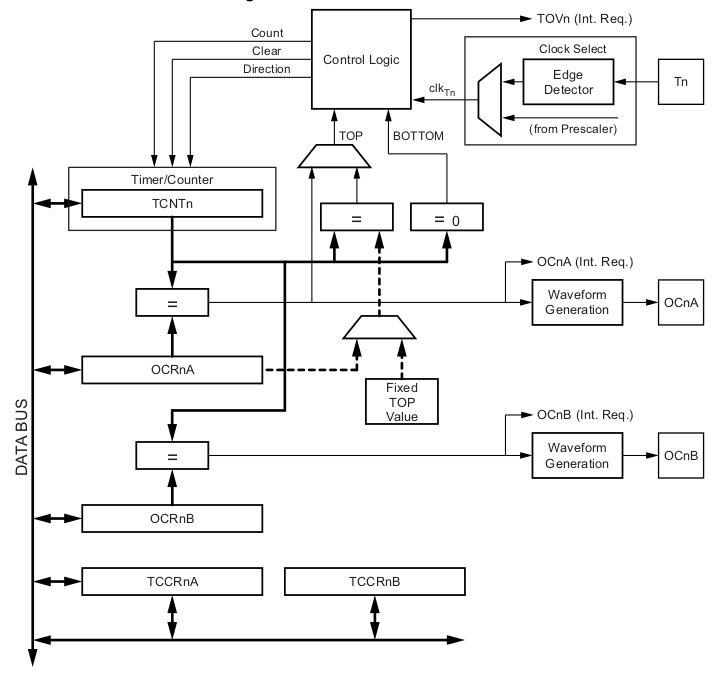
\includegraphics[height=0.6\textheight]{Timer0BlockDiagram.png}
    \end{center}
\end{figure}

\section{Terminologies and Registers}
\begin{minipage}{0.45\textwidth}
    \begin{tabular}{c|p{5.5cm}}
        \textbf{Parameter} & \textbf{Description}\\
        \hline
        BOTTOM & counter reaches 0x00\\
        MAX & ounter reaches 0xFF\\
        TOP & counter reaches highest value (depends on mode of operation can be 0xFF, OCR2A).        
    \end{tabular}
\end{minipage}
\begin{minipage}{0.5\textwidth}
    \begin{tabular}{c|p{6cm}}
        \textbf{Register - 8 bit} & \textbf{Name}\\
        \hline
        \regFormat{TCNT2} & Timer/Counter2 count value\\
        \regFormat{TCCR2A} & Timer/Counter2 Control Register A\\
        \regFormat{TCCR2B} & Timer/Counter2 Control Register B\\
        \regFormat{OCBR2A} & Output compare register A\\
        \regFormat{OCBR2B} & Output compare register B\\
        \regFormat{TIFR2} & Timer Interrupt Flag Register\\
        \regFormat{TIMSK2} & Timer interrupt Mask Register\\
    \end{tabular}
\end{minipage}

\section{Timer/Counter2 Units}
\subsection{Clock Source/Select Unit}
\begin{figure}[H]
    \begin{center}
        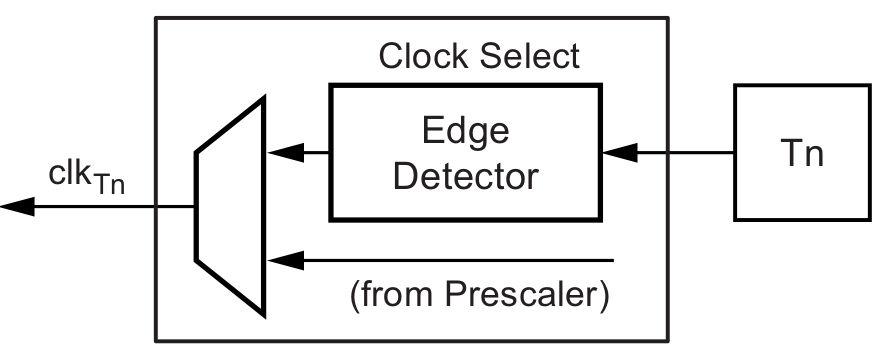
\includegraphics[width=0.5\textwidth]{Timer0ClockSelector.png}
    \end{center}
\end{figure}
\begin{itemize}
    \item The source for the Timer/Counter2 can be external or internal.
    \item External clock source is from \pinFormat{T2} pin.
    \item While Internal Clock source can be clocked via a prescalar.
    \item The output of this unit is the timer clock ($clk_{T2}$).
    \item It uses \bitFormat{CS2[2:0]} bits in \regFormat{TCCR2B} register to select the source.
\end{itemize}


\subsection{Counter Unit}
\begin{minipage}{0.5\textwidth}
    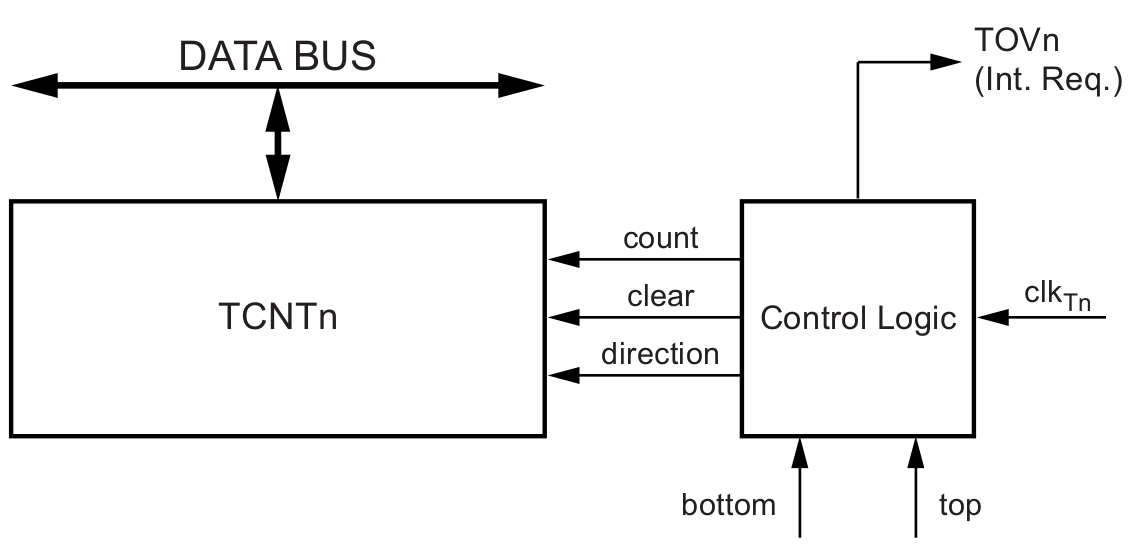
\includegraphics[width=1\textwidth]{Timer0CounterUnit.png}
\end{minipage}
\begin{minipage}{0.45\textwidth}
    \begin{tabular}{c|p{5.5cm}}
        \textbf{Signal} & \textbf{Description}\\
        \hline  
        count & Increment or decrement \regFormat{TCNT2} by 1\\
        direction & Select between increment or decrement\\
        clear & Clears \regFormat{TCNT2} to 0x00\\
        $clk_{T2}$ & Timer/Counter2 clock\\
        top & Signalize that \regFormat{TCNT2} has maximum value\\
        bottom & Signalize that \regFormat{TCNT2} has minimum value(0x00)\\
    \end{tabular}
\end{minipage}
\begin{itemize}
    \item The main part of the 8-bit Timer/Counter is the programmable bi-directional counter.
    \item Depending the mode of operation the counter is cleared, incremented, or decremented at each timer clock ($clk_{T2}$).
    \item Counting sequence is determined by \bitFormat{WGM2[1:0]} bits of \regFormat{TCCR2A} -Timer/Counter2 Control register A and \bitFormat{WGM22} bit of \regFormat{TCCR2B} - Timer/Counter2 Control register B.
    \item The Timer/Counter2 Overflow flag \bitFormat{TOV2} is set and can generate interrupt according to the mode.
\end{itemize}


\subsection{Output Compare Unit}
\begin{figure}[H]
    \begin{center}
        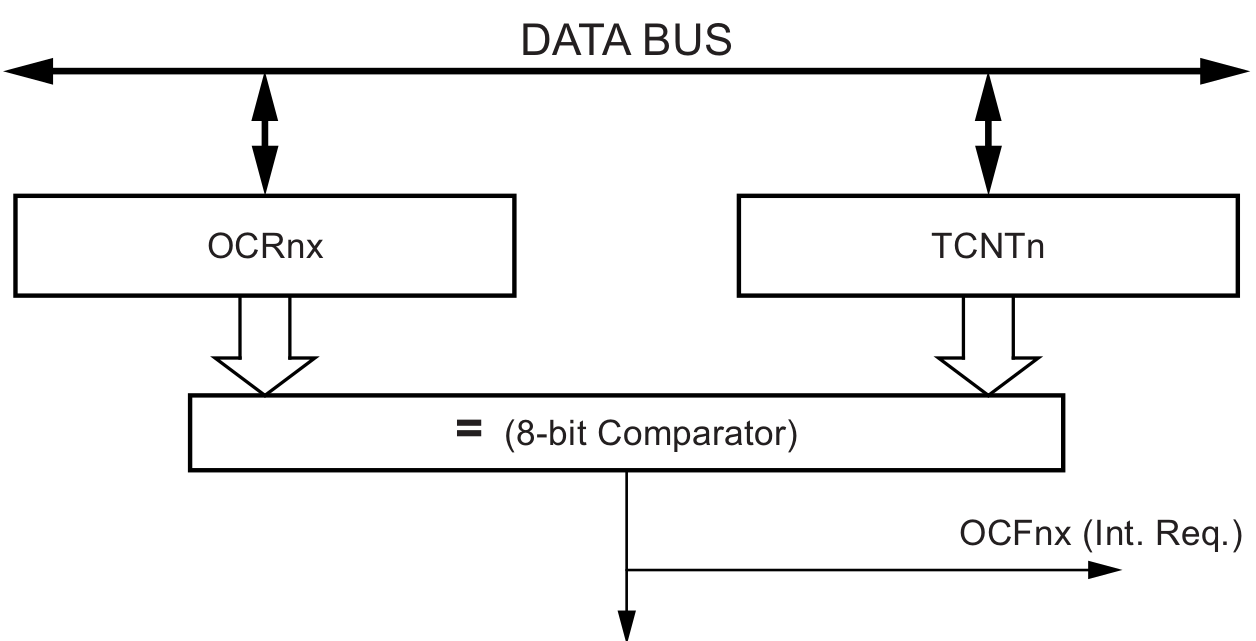
\includegraphics[width=0.5\textwidth]{Timer0CompareUnit.png}
    \end{center}
\end{figure}
\begin{itemize}
    \item 8-bit comparator continuously compares \regFormat{TCNT2} with both \regFormat{OCR2A} and \regFormat{OCR2B}.
    \item When \regFormat{TCNT2} equals \regFormat{OCR2A} or \regFormat{OCR2B}, the comparator signals a match which will set the output compare flag at the next timer clock cycle.
    \item If interrupts are enabled, then output compare interrupt is generated.
    \item The waveform generator uses the match signal to generate an output according to operating mode set by the \bitFormat{WGM2[2:0]} bits and compare output mode \bitFormat{COM2x[1:0]} bits.
\end{itemize}

\subsection{Compare Match Output Unit}
\begin{figure}[H]
    \begin{center}
        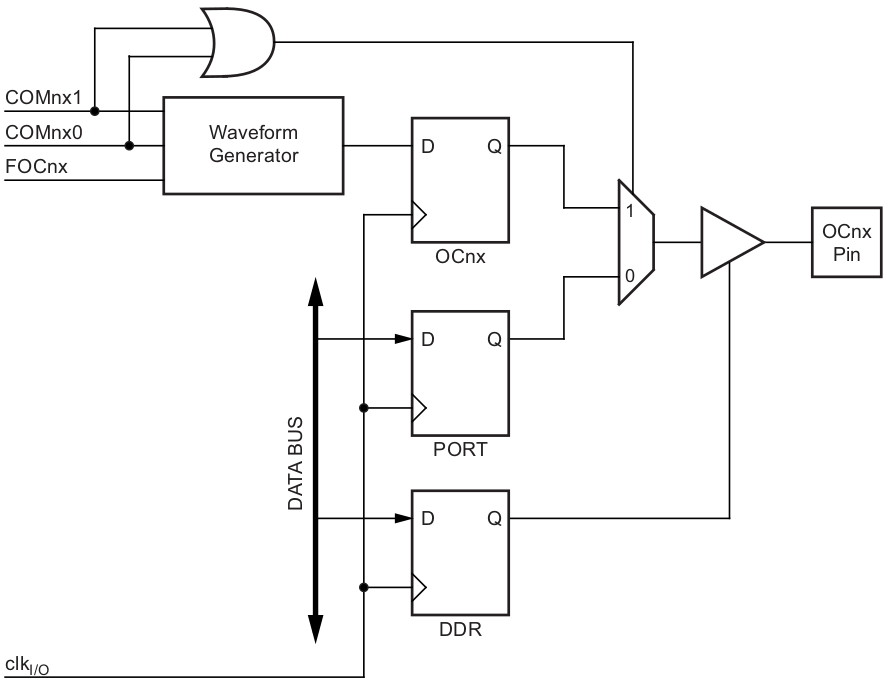
\includegraphics[height=0.3\textheight]{Timer0ComparteMatch.png}
    \end{center}
\end{figure}
\begin{itemize}
    \item This unit is used for changing the state of \pinFormat{OC2A} and \pinFormat{OC2B} pins by configuring the \bitFormat{COM2x[1:0]} bits.
    \item But, general I/O port function is overriiden by DDR reigster.
\end{itemize}

\section{Modes of Operation}
\begin{itemize}
    \item The mode of operation can be defined by combination of waveform generation mode (\bitFormat{WGM2[2:0]}) and compare output mode(\bitFormat{COM2[1:0]}) bits.
    \item The waveform generation mode (\bitFormat{WGM2[2:0]}) bits affect the counting sequence.
    \item For non-PWM mode, \bitFormat{COM2[1:0]} bits control if the output should be set, cleared or toggled at a compare match.
    \item For PWM mode, \bitFormat{COM2[1:0]} bits control if the PWM generated should be inverted or non-inverted.
\end{itemize}

\subsection{Normal Mode - Non-PWM Mode}
\begin{itemize}
    \item \bitFormat{WGM2[2:0]} $-->$ 000.
    \item Counter counts up and no counter clear.
    \item Overruns TOP(0XFF) and restarts from BOTTOM(0X00).
    \item \bitFormat{TOV2} Flag is only set when overrun.
    \item We have to clear \bitFormat{TOV2} flag inorder to have next running.
    \item But, if we use interrupt we don’t need to clear it as interrupt automatically clear the \bitFormat{TOV2} flag.
    \item The timing can be seen below.
\end{itemize}

\begin{tikztimingtable}[
    timing/dslope=0.1,
    timing/.style={x=5ex,y=2ex},
    x=5ex,
    timing/rowdist=3ex,
    timing/name/.style={font=\sffamily\scriptsize}
    ]
    \busref{clk\_{T2}}  & 41{c}\\
    \busref{TCNT2} & u{} D{0x00} D{0x01};[dotted] 2D{};D{0xFE} D{0xFF}D{0x00} D{0x01};[dotted] 2D{};D{0xFE} D{0xFF}D{0x00} D{0x01};[dotted] 2D{};D{0xFE} D{0xFF}D{0x00} D{0x01}\\
    \busref{TOV2} & l 6{L} H 5{L} H 5{L} H 1{L}\\
\end{tikztimingtable}

\subsection{Clear Timer on Compare Match(CTC) Mode - Non-PWM Mode}
\begin{itemize}
    \item \bitFormat{WGM2[2:0]} $-->$ 010.
    \item Counter value clears when \regFormat{TCNT2} reaches \regFormat{OCR2A}.
    \item Interrupt can be generated each time \regFormat{TCNT2} reaches \regFormat{OCR2A} register value by \bitFormat{OCF0A} flag.
    \item When \bitFormat{COM2A[1:0]} == 01, the \pinFormat{OC2A} pin output can be set to toggle its match between \regFormat{TCNT2} and \regFormat{OCR2A} to generate waveform.
    \item The frequency of the waveform its
    \begin{center}
        { \Large $f_{OC2A} = \frac{f_{clkT2}}{2 * N * (1 + OCR2A)}$ }
    \end{center}
    \item Here N is prescalar factor and can be (1, 8, 64, 256, or 1024).
\end{itemize}
\begin{tikztimingtable}[
    timing/dslope=0.1,
    timing/.style={x=5ex,y=2ex},
    x=5ex,
    timing/rowdist=3ex,
    timing/name/.style={font=\sffamily\scriptsize}
    ]
    \busref{clk\_{T2}}  & 28{1.5c}\\
    \busref{TCNT2} & 0.75U{} 1.5D{0x00} 1.5D{0x01};[dotted] 3D{};1.5D{OCR2A - 1} 1.5D{OCR2A}1.5D{0x00} 1.5D{0x01};[dotted] 3D{};1.5D{OCR2A - 1} 1.5D{OCR2A} 1.5D{0x00} 0.75D{0x01} \\
    \busref{OC2A} & 0.75L 9{L} 1.5H l 7{L} 1.5H l\\
\end{tikztimingtable}

\subsection{Fast PWM Mode}
\begin{itemize}
    \item \bitFormat{WGM2[2:0]} $-->$ 011 or 111.
    \item Power Regulation, Rectification, DAC applications.
    \item Single slope operations causing high frequency PWM waveform.
    \item Counter starts from BOTTOM to TOP and then restarts from BOTTOM.
    \item TOP is defined by
    \begin{itemize}
        \item TOP == 0xFF if \bitFormat{WGM2[2:0]} $-->$ 011
        \item TOP == \regFormat{OCR2A} if \bitFormat{WGM2[2:0]} $-->$ 111
    \end{itemize}
    \item  When \bitFormat{COM2A[1:0]} == 01, the \pinFormat{OC2A} pin output can be set to toggle its match between \regFormat{TCNT2} and TOP to generate waveform.
    \begin{itemize}
        \item The above is possible only when \bitFormat{WGM22} bit is set.
        \item And only on \pinFormat{OC2A} pin and not on \pinFormat{OC2B} pin.
    \end{itemize}
    \item In Inverting Compare Mode \bitFormat{COM2A[1:0]} == 10 , the \pinFormat{OC2A} or \pinFormat{OC2B} pins is made 1 on compare match between \regFormat{TCNT2} and TOP and made 0 on reaching BOTTOM.
    \item In Non-Inverting Compare Mode \bitFormat{COM2A[1:0]} == 11 , the \pinFormat{OC2A} or \pinFormat{OC2B} pins is made 0 on compare match between \regFormat{TCNT2} and TOP and 1 made  on reaching BOTTOM.
    \item The Timer/Counter overflow flag (\bitFormat{TOV2}) is set each time the counter reaches TOP.
    \item The PWM frequency is given by 
    \begin{center}
        { \Large $f_{OC0xPWM} = \frac{f_{clkT2}}{N * 256}$ }
    \end{center}
\end{itemize}

\subsubsection{WGM[2:0] == 011}
\begin{tikztimingtable}[
    timing/dslope=0.1,
    timing/.style={x=5ex,y=2ex},
    x=5ex,
    timing/rowdist=3ex,
    timing/name/.style={font=\sffamily\scriptsize}
    ]
    \busref{clk\_{T2}}  & 41{1c} c\\
    \busref{TCNT2} & 0.5U{} D{0x00} 1D{0x01};[dotted] 1.5D{};1D{0xFE} 1D{0xFF}1D{0x00} 1D{0x01};[dotted] 1D{};1D{0xFE} 1D{0xFF} 1D{0x00} 1D{0x01} [dotted] 1D{};1D{0xFE} 1D{0xFF} 1D{0x00} 1D{0x01};[dotted] 1D{};1D{0xFE} 1D{0xFF};\\
    \busref{TOV2} & 6{L} H 4{L} H 4{L} H 4{L} \\
\end{tikztimingtable}

\subsubsection{WGM[2:0] == 011}
\begin{tikztimingtable}[
    timing/dslope=0.1,
    timing/.style={x=5ex,y=2ex},
    x=5ex,
    timing/rowdist=3ex,
    timing/name/.style={font=\sffamily\scriptsize}
    ]
    \busref{clk\_{T2}}  & 41{1c} c\\
    \busref{TCNT2} & 0.5U{} D{0x00} 1D{0x01};[dotted] 1.5D{};1D{\tiny OCR2A -1} 1D{\tiny OCR2A}1D{0x00} 1D{0x01};[dotted] 1D{};1D{\tiny OCR2A -1} 1D{\tiny OCR2A} 1D{0x00} 1D{0x01} [dotted] 1D{};1D{\tiny OCR2A -1} 1D{\tiny OCR2A} 1D{0x00} 1D{0x01};[dotted] 1D{};1D{\tiny OCR2A -1} 1D{\tiny OCR2A};\\
    \busref{TOV2} & 6{L} H 4{L} H 4{L} H 4{L} \\
\end{tikztimingtable}


\subsection{Phase Correct PWM Mode}
\begin{itemize}
    \item \bitFormat{WGM2[2:0]} $-->$ 001 or 101.
    \item High resolution phase correct PWM.
    \item Motor control due to symmetric features
    \item Dual slope operations causing ower frequency PWM waveform.
    \item Counter starts from BOTTOM to TOP and then from TOP to BOTTOM.
    \item TOP is defined by
    \begin{itemize}
        \item TOP == 0xFF if \bitFormat{WGM2[2:0]} $-->$ 001
        \item TOP == \regFormat{OCR2A} if \bitFormat{WGM2[2:0]} $-->$ 101
    \end{itemize}
    \item  When \bitFormat{COM2A[1:0]} == 01, the \pinFormat{OC2A} pin output can be set to toggle its match between \regFormat{TCNT2} and TOP to generate waveform.
    \begin{itemize}
        \item The above is possible only when \bitFormat{WGM22} bit is set.
        \item And only on \pinFormat{OC2A} pin and not on \pinFormat{OC2B} pin.
    \end{itemize}
    \item In Inverting Compare Mode \bitFormat{COM2A[1:0]} == 10 , the \pinFormat{OC2A} or \pinFormat{OC2B} pins is made 1 on compare match between \regFormat{TCNT2} and TOP and made 0 on reaching BOTTOM.
    \item In Non-Inverting Compare Mode \bitFormat{COM2A[1:0]} == 11 , the \pinFormat{OC2A} or \pinFormat{OC2B} pins is made 0 on compare match between \regFormat{TCNT2} and TOP and 1 made  on reaching BOTTOM.
    \item The Timer/Counter overflow flag (\bitFormat{TOV2}) is set each time the counter reaches BOTTOM..
    \item The PWM frequency is given by 
    \begin{center}
        { \Large $f_{OC0xPWM} = \frac{f_{clkT2}}{N * 510}$ }
    \end{center}
\end{itemize}

\subsubsection{WGM[2:0] == 001}
\begin{tikztimingtable}[
    timing/dslope=0.1,
    timing/.style={x=5ex,y=2ex},
    x=5ex,
    timing/rowdist=3ex,
    timing/name/.style={font=\sffamily\scriptsize}
    ]
    \busref{clk\_{T2}}  & 41{1c}\\
    \busref{TCNT2} & 0.5U{} D{0x00} 1D{0x01};[dotted] 1.5D{};1D{0xFE} 1D{0xFF}1D{0xFE} 1D{0xFD};[dotted] 1D{};1D{0x01} 1D{0x00} 1D{0x01}[dotted] 1D{};1D{0xFE} 1D{0xFF} 1D{0xFE} 1D{0xFD};[dotted] 1D{};1D{0x01} 1D{0x00} 1d{0x01};\\
    \busref{TOV2} & l H l 8{L} H 8{L} H l\\
\end{tikztimingtable}

\subsubsection{WGM[2:0] == 101}
\begin{tikztimingtable}[
    timing/dslope=0.1,
    timing/.style={x=5ex,y=2ex},
    x=5ex,
    timing/rowdist=3ex,
    timing/name/.style={font=\sffamily\scriptsize}
    ]
    \busref{clk\_{T2}}  & 41{1c}\\
    \busref{TCNT2} & 0.5U{} D{0x00} 1D{0x01};[dotted] 1.5D{};1D{\tiny OCR2A - 1} 1D{\tiny OCR2A}1D{\tiny OCR2A-1} 1D{\tiny OCR2A-2};[dotted] 1D{};1D{0x01} 1D{0x00} 1D{0x01}[dotted] 1D{};1D{\tiny OCR2A-1} 1D{\tiny OCR2A} 1D{\tiny OCR2A-1} 1D{\tiny OCR2A-2};[dotted] 1D{};1D{0x01} 1D{0x00} 1d{0x01};\\
    \busref{TOV2} & l H l 8{L} H 8{L} H l\\
\end{tikztimingtable}
\newpage
\section{Register Description}
\subsubsection*{TCCR2A – Timer/Counter Control Register A}
\vspace*{0.5cm}
\begin{bytefield}[bitformatting={\large\bfseries},
    endianness=big,bitwidth=0.125\linewidth]{8}
    \bitheader[lsb=0]{0-7} \\
    \bitbox{1}{\small COM2A1}
    \bitbox{1}{\small COM2A0}
    \bitbox{1}{\small COM2B1}
    \bitbox{1}{\small COM2B0}
    \bitbox{1}{\small -}
    \bitbox{1}{\small -}
    \bitbox{1}{\small WGM21}
    \bitbox{1}{\small WGM20}\\
\end{bytefield}

\begin{table}[H]
    \begin{center}
        \begin{tabular}{c|p{4cm}|p{5.2cm}|p{5.2cm}}
            \bitFormat{COM2B[1:0]} & \textbf{Non-PWM modes} & \textbf{Fast PWM} & \textbf{Phase Corrected PWM}\\
            \hline
            00 & No output @ \pinFormat{PD3 - OC2B} pin &  No output @ \pinFormat{PD3 - OC2B} & No output @ \pinFormat{PD3 - OC2B}\\
            \hline
            01 & Toggle \pinFormat{PD3 - OC2B} pin on compare Match. & Reserved & Reserved\\
            \hline
            10 & Clear \pinFormat{PD3 - OC2B} pin on compare Match. & Clear \pinFormat{PD3 - OC2B} on compare match and  set \pinFormat{PD3 - OC2B} at BOTTOM & Clear \pinFormat{PD3 - OC2B} on compare match when up-counting and set \pinFormat{PD3 - OC2B} on compare match when down-counting.\\
            \hline
            11 & Set \pinFormat{PD3 - OC2B} pin on compare Match. & Set \pinFormat{PD3 - OC2B} on compare match and clear \pinFormat{PD3 - OC2B} at BOTTOM & Set \pinFormat{PD3 - OC2B} on compare match when up-counting and clear \pinFormat{PD3 - OC2B} on compare match when down-counting\\
        \end{tabular}
    \end{center}
\end{table}

\begin{table}[H]
    \begin{center}
        \begin{tabular}{c|p{4cm}|p{5.2cm}|p{5.2cm}}
            \bitFormat{COM2A[1:0]} & \textbf{Non-PWM modes} & \textbf{Fast PWM} & \textbf{Phase Corrected PWM}\\
            \hline
            00 & No output @ \pinFormat{PB3 - OC2A} pin &  No output @ \pinFormat{PB3 - OC2A} & No output @ \pinFormat{PB3 - OC2A}\\
            \hline
            01 & Toggle \pinFormat{PB3 - OC2A} pin on compare Match. & When WGM2[2] == 1, Toggle \pinFormat{PB3 - OC2A}  pin on Compare match & Toggle \pinFormat{PB3 - OC2A}  pin on Compare match\\
            \hline
            10 & Clear \pinFormat{PB3 - OC2A} pin on compare Match. & Clear \pinFormat{PB3 - OC2A} on compare match and  set \pinFormat{PB3 - OC2A} at BOTTOM & Clear \pinFormat{PB3 - OC2A} on compare match when up-counting and set \pinFormat{PB3 - OC2A} on compare match when down-counting.\\
            \hline
            11 & Set \pinFormat{PB3 - OC2A} pin on compare Match. & Set \pinFormat{PB3 - OC2A} on compare match and  clear \pinFormat{PB3 - OC2A} at BOTTOM & Set \pinFormat{PB3 - OC2A} on compare match when up-counting and clear \pinFormat{PB3 - OC2A} on compare match when down-counting\\
        \end{tabular}
    \end{center}
\end{table}

\begin{table}[H]
    \begin{center}
        \begin{tabular}{c|c|c|c}
            \bitFormat{WGM2[2:0]} & \textbf{Mode of operation} & \textbf{TOP} & \textbf{TOV2 Flag set on}\\
            \hline
            000 & Normal & 0xFF & MAX\\
            001 & PWM Phase Corrected & 0xFF & BOTTOM\\
            010 & CTC & OCRA & MAX\\
            011 & Fast PWM & 0xFF & MAX\\
            101 & PWM Phase Corrected & OCR2A  & BOTTOM\\
            111 & Fast PWM & OCR2A & TOP\\
        \end{tabular}
    \end{center}
\end{table}

\subsubsection*{TCCR2B – Timer/Counter Control Register B}
\vspace*{0.5cm}
\begin{bytefield}[bitformatting={\large\bfseries},
    endianness=big,bitwidth=0.125\linewidth]{8}
    \bitheader[lsb=0]{0-7} \\
    \bitbox{1}{\small FOC2A}
    \bitbox{1}{\small FOC2B}
    \bitbox{1}{\small -}
    \bitbox{1}{\small -}
    \bitbox{1}{\small WGM22}
    \bitbox{1}{\small CS22}
    \bitbox{1}{\small CS21}
    \bitbox{1}{\small CS20}\\
\end{bytefield}

\begin{table}[H]
    \begin{center}
        \begin{tabular}{c|c}
            \bitFormat{CS2[2:0]} & \textbf{Description(Prescalar)}\\
            \hline
            000 & No clock source(Timer/Counter Stopped)\\
            001 & $clk_{I/O}$ – no prescaling\\
            010 & $\frac{clk_{I/O}}{8}$\\
            011 & $\frac{clk_{I/O}}{64}$\\\
            100 & $\frac{clk_{I/O}}{256}$\\\
            101 & $\frac{clk_{I/O}}{1024}$\\\
            110 & External clock source on \pinFormat{T2} pin. Clock on falling edge.\\
            111 & External clock source on \pinFormat{T2} pin. Clock on rising edge.\\
        \end{tabular}
    \end{center}
\end{table}

\subsubsection*{TIMSK2 – Timer/Counter Interrupt Mask Register}
\vspace*{0.5cm}
\begin{bytefield}[bitformatting={\large\bfseries},
    endianness=big,bitwidth=0.125\linewidth]{8}
    \bitheader[lsb=0]{0-7} \\
    \bitbox{1}{\small -}
    \bitbox{1}{\small -}
    \bitbox{1}{\small -}
    \bitbox{1}{\small -}
    \bitbox{1}{\small -}
    \bitbox{1}{\small OCIE2B}
    \bitbox{1}{\small OCIE2A}
    \bitbox{1}{\small TOIE2}\\
\end{bytefield}

\quad Enable interrupts for compare match between \regFormat{TCNT2} and \regFormat{OCR2A} or \regFormat{TCNT2} and \regFormat{OCR2B} or overflow in \regFormat{TCNT2}.

\subsubsection*{TIFR2 – Timer/Counter 0 Interrupt Flag Register}
\vspace*{0.5cm}
\begin{bytefield}[bitformatting={\large\bfseries},
    endianness=big,bitwidth=0.125\linewidth]{8}
    \bitheader[lsb=0]{0-7} \\
    \bitbox{1}{\small -}
    \bitbox{1}{\small -}
    \bitbox{1}{\small -}
    \bitbox{1}{\small -}
    \bitbox{1}{\small -}
    \bitbox{1}{\small OCIE2B}
    \bitbox{1}{\small OCIE2A}
    \bitbox{1}{\small TOIE2}\\
\end{bytefield}

\quad FLag registers for interrupts on compare match between \regFormat{TCNT2} and \regFormat{OCR2A} or \regFormat{TCNT2} and \regFormat{OCR2B} or overflow in \regFormat{TCNT2}.
\newpage


\section{Configuring the Timer/Counter}
\subsection{Normal Mode}
\subsubsection{As Timer}
\begin{center}
    $ON\_TIME = \frac{max\_count}{\frac{F\_CPU}{PRESCALAR}}$
\end{center}
\begin{itemize}
    \item Depending on PRESCALR value, we get different ON\_TIME.
    \item First, \bitFormat{WGM2[2:0]} bits are configured as 000 for Normal Mode in \regFormat{TCCR2A} and \regFormat{TCCR2B} registers.
    \item Next, \bitFormat{COM2A[1:0]} and/or \bitFormat{COM2A[1:0]} bits are configured to make outputs \pinFormat{OC2A} and/or \pinFormat{OC2B} pins to do nothing, set, clear or toggle in \regFormat{TCCR2A} register.
    \item Next, Interrupt is Enabled by \bitFormat{TOIE2} (overflow enable) in \regFormat{TIMSK2} reigster.
    \item Finally, Timer is started by setting prescalar in \bitFormat{CS2[2:0]} bits as needed prescalar of \regFormat{TCR2B} reigster.
    \item Global Interrupt is enabled.
    \item A interrupt Service Routine for Timer2 overflow is Written.
    \item No need to clear the overflow flag as it is done by hardware.
    \item The timing when both pins \pinFormat{OC2A} and \pinFormat{OC2B} are made to toggle.
\end{itemize}

\begin{tikztimingtable}[
    timing/dslope=0.1,
    timing/.style={x=5ex,y=2ex},
    x=5ex,
    timing/rowdist=3ex,
    timing/name/.style={font=\sffamily\scriptsize}
    ]
    \busref{clk\_{T2}}  & 41{c}\\
    \busref{TCNT2} & u{} D{0x00} D{0x01};[dotted] 2D{};D{0xFE} D{0xFF}D{0x00} D{0x01};[dotted] 2D{};D{0xFE} D{0xFF}D{0x00} D{0x01};[dotted] 2D{};D{0xFE} D{0xFF}D{0x00} D{0x01}\\
    \busref{TOV2} & u h h 5{L} H 5{L} H 5{L} H 1{L}\\
    \busref{OC2A} & l H 5{H} 6{L} 6{H} 2{L}\\
    \busref{OC2B} & h L 5{L} 6{H} 6{L} 2{H}\\
\end{tikztimingtable}
\begin{itemize}
    \item The code can be seen below,
\end{itemize}
\begin{minted}[breaklines,bgcolor=lightgray]{c}
// MOde of operation to Normal Mode -- WGM2[2:0] === 000
// WGM2[2](bit3) from TCCR2B, WGM2[1](bit1)  from TCCR2A, WGM2[0](bit0)  from TCCR2A
TCCR2A = TCCR2A & (~(1<<0) & ~(1<<1));
TCCR2B = TCCR2B & ~(1<<3);

/* What to do when timer reaches the MAX(0xFF) value */	
// toggle OC2A and OC2B on each time when reaches the MAX(0xFF) 
// which is reflected in PB3 and PD3

// Output OC2A to toglle when reaches MAX -- COM2A[1:0] === 01
// COM2A[1](bit7) from TCCR2A, COM2A[0](bit6) from TCCR2A
TCCR2A = TCCR2A & ~(1<<7);
TCCR2A = TCCR2A | (1<<6);

// Output OC2B to toglle when reaches MAX -- COM2B1:0] === 01
// COM2B[1](bit7) from TCCR2A, COM2B[0](bit6) from TCCR2A
TCCR2A = TCCR2A & ~(1<<5);
TCCR2A = TCCR2A | (1<<4);

//Enable Interrupt of OVERFLOW flag so that interrupt can be generated
TIMSK2 = TIMSK2 | (1<<0);	

// start timer by setting the clock prescalar
// DIVIDE BY 8 from I/O clock
// DIVIDE BY 8-- CS2[2:0] === 010
// CS2[2](bit2) from TCCR2B,CS2[1](bit1) from TCCR2B,CS2[0](bit0) from TCCR2B
TCCR2B = TCCR2B | (1<<1);
TCCR2B = TCCR2B & (~(1<<0) & ~(1<<2));

// enabling global interrupt
sei();
// SO ON TIME = max_count / (F_CPU / PRESCALAR)
// ON TIME = 0xFF / (16000000/8) = 128us
// since symmetric as toggling OFF TIME = 128us
// hence, we get a square wave of fequency 1 / 256us = 3.906kHz
\end{minted}

\begin{minted}[breaklines,bgcolor=lightgray]{c}
ISR(TIMER2_OVF_vect)
{
    // do the thing when overflows.
}
\end{minted}



\subsubsection{Application I - Delay}
\begin{minted}[breaklines,bgcolor=lightgray]{c}
/* TCNT2 starts from 0X00 goes upto 0XFF and restarts */
/* No possible use case as it just goes upto 0xFF and restarts */
// MOde of operation to Normal Mode -- WGM2[2:0] === 000
// WGM2[2](bit3) from TCCR2B, WGM2[1](bit1)  from TCCR2A, WGM2[0](bit0)  from TCCR2A
TCCR2A = TCCR2A & (~(1<<0) & ~(1<<1));
TCCR2B = TCCR2B & ~(1<<3);

/* What to do when timer reaches the MAX(0xFF) value */
// nothing should be done on OC2A for delay
// nothing  -- COM2A[1:0] === 00
// COM2A[1](bit7) from TCCR2A, COM2A[0](bit6) from TCCR2A
TCCR2A = TCCR2A & ~(1<<7);
TCCR2A = TCCR2A & ~(1<<6);
    
/* The delay possible = 0xff / (F_CPU/prescalar) */
// lowest delay = 0xff / (16000000 / 1) = 16us
// when prescalar == 8 --> delay = 0xff / (16000000 / 8) = 128us
// when prescalar == 64 --> delay = 0xff / (16000000 / 64) = 1.024ms
// when prescalar == 256 --> delay = 0xff / (16000000 / 256) = 4.096ms
// highest delay possible = 0xff / (16000000 / 1024) = 16.38ms

// start timer by setting the clock prescalar
// DIVIDE BY 8 use the same clock from I/O clock
// DIVIDE BY 8-- CS2[2:0] === 010
// CS2[2](bit2) from TCCR2B,CS2[1](bit1) from TCCR2B,CS2[0](bit0) from TCCR2B
TCCR2B = TCCR2B & ~(1<<0);
TCCR2B = TCCR2B | (1<<1);
TCCR2B = TCCR2B & ~(1<<2);


// actual delaying - wait until delay happens
while((TIFR2 & 0x01) == 0x00); // checking overflow flag when overflow happns
// clearing the overflag so that we can further utilize
TIFR2 = TIFR2 | 0x01;
\end{minted}

\subsection{CTC Mode}
\subsubsection{As Timer}

\begin{center}
    $ON\_TIME = \frac{1 + OCR2A}{\frac{F\_CPU}{PRESCALAR}}$
\end{center}
\begin{itemize}
    \item Depending on \regFormat{OCR2A} register and PRESCALR value, we get different ON\_TIME.
    \item First, \bitFormat{WGM2[2:0]} bits are configured as 010 for CTC Mode in \regFormat{TCCR2A} and \regFormat{TCCR2B} registers.
    \item Next, \bitFormat{COM2A[1:0]} and/or \bitFormat{COM2B[1:0]} bits are configured to make outputs \pinFormat{OC2A} and/or \pinFormat{OC2B} pins to do nothing, set, clear or toggle in \regFormat{TCCR2A} register.
    \item Next, Interrupt is Enabled by \bitFormat{OCIE01A} (utput compare on match on \regFormat{OCR2A} register enable) in \regFormat{TIMSK2} reigster.
    \item Finally, Timer is started by setting prescalar in \bitFormat{CS2[2:0]} bits as needed prescalar of \regFormat{TCR2B} reigster.
    \item Global Interrupt is enabled.
    \item A interrupt Service Routine for TIMER2 Compare is Written.
    \item No need to clear the overflow flag as it is done by hardware.
    \item The timing when both pins \pinFormat{OC0n} are made to toggle.
\end{itemize}


\begin{tikztimingtable}[
    timing/dslope=0.1,
    timing/.style={x=5ex,y=2ex},
    x=5ex,
    timing/rowdist=3ex,
    timing/name/.style={font=\sffamily\scriptsize}
    ]
    \busref{clk\_{T2}}  & 41{c}\\
    \busref{TCNT2} & u{} D{0x00} D{0x01};[dotted] 2D{};D{\tiny OCR2A - 1} D{\tiny OCR2A}D{0x00} D{0x01};[dotted] 2D{};D{\tiny OCR2A - 1} D{\tiny OCR2A }D{0x00} D{0x01};[dotted] 2D{};D{\tiny OCR2A - 1} D{\tiny OCR2A}D{0x00} D{0x01}\\
    \busref{TOV2} & u h h 5{L} H 5{L} H 5{L} H 1{L}\\
    \busref{OC2A} & l H 5{H} 6{L} 6{H} 2{L}\\
    \busref{OC2B} & h L 5{L} 6{H} 6{L} 2{H}\\
\end{tikztimingtable}
\begin{itemize}
    \item The code can be seen below,
\end{itemize}
\begin{minted}[breaklines,bgcolor=lightgray]{c}
// MOde of operation to CTC Mode -- WGM2[2:0] === 010
// WGM2[2](bit3) from TCCR2B, WGM2[1](bit1)  from TCCR2A, WGM2[0](bit0)  from TCCR2A
TCCR2A = TCCR2A & ~(1<<0);
TCCR2A = TCCR2A | (1<<1);
TCCR2B = TCCR2B & ~(1<<3);

/* What to do when timer reaches the OCR2A */
// toggle OC2A on each time when reaches the OCR2A
// which is reflected in PB3
// Output OC2A to toglle when reaches MAX -- COM2A[1:0] === 01
// COM2A[1](bit7) from TCCR2A, COM2A[0](bit6) from TCCR2A
TCCR2A = TCCR2A & ~(1<<7);
TCCR2A = TCCR2A | (1<<6);

// Output OC2B to toglle when reaches MAX -- COM2B1:0] === 01
// COM2B[1](bit7) from TCCR2A, COM2B[0](bit6) from TCCR2A
TCCR2A = TCCR2A & ~(1<<5);
TCCR2A = TCCR2A | (1<<4);

    
// Enable Interrupt when counter matches OCR2A Rgister
//  OCIE2A bit is enabled
TIMSK2 = TIMSK2 | (1<<1);


// setting the value till the counter should reach in OCR2A
// for toggling of OC2A pin
OCR2A = 0x32;

// start timer by setting the clock prescalar
// DIVIDE BY 8 from I/O clock
// DIVIDE BY 8-- CS2[2:0] === 010
// CS2[2](bit2) from TCCR2B,CS2[1](bit1) from TCCR2B,CS2[0](bit0) from TCCR2B
TCCR2B = TCCR2B | (1<<1);
TCCR2B = TCCR2B & (~(1<<0) & ~(1<<2));

// enabling global interrupt
sei();
// SO ON TIME = (1 + OCR2A) / (F_CPU / PRESCALAR)
// ON TIME = 0X32 / (16000000/8) = 25.5us
// since symmetric as toggling OFF TIME = 25.5us
// hence, we get a square wave of fequency 1 / 50us = 20kHz
\end{minted}

\begin{minted}[breaklines,bgcolor=lightgray]{c}
ISR(TIMER2_COMPA_vect)
{
    // do the thing when compare match between TCNT2 matches OCR2A.
}
\end{minted}



\subsubsection{Application I - Delay in ms}

\begin{minted}[breaklines,bgcolor=lightgray]{c}
// minimum delay being 4us -- choose like that
// use PRESCALAR OF 1 -- 3us - 16us -- usage 3us - 16us -- factor=0 -- CS2[2:0]=1
// use PRESCALAR OF 8 -- 3us - 128us -- usage 17us - 128us -- factor=3 -- CS2[2:0]=2
// use PRESCALAR OF 64 -- 4us - 1.024ms -- usage 129us - 1024us -- factor=6 -- CS2[2:0]=3
// use PRESCALAR OF 256 -- 16us - 4.096ms -- usage 1025us - 4096us -- factor=8 -- CS2[2:0]=4
    
// MOde of operation to ctc Mode -- WGM2[2:0] === 010
// WGM2[2](bit3) from TCCR2B, WGM2[1](bit1)  from TCCR2A, WGM2[0](bit0)  from TCCR2A
TCCR2A = TCCR2A & ~(1<<0);
TCCR2A = TCCR2A | (1<<1);
TCCR2B = TCCR2B & ~(1<<3);

while(delayInMs--)
{
    // for 1ms delay
    OCR2A = 249;
    // start timer by setting the clock prescalar
    //  dived by 64 from I/O clock
    //  CS2[2:0] === 011
    // CS2[2](bit2) from TCCR2B,CS2[1](bit1) from TCCR2B,CS2[0](bit0) from TCCR2B
    TCCR2B = TCCR2B | (1<<0);
    TCCR2B = TCCR2B | (1<<1);
    TCCR2B = TCCR2B & ~(1<<2);

    // actual delaying - wait until delay happens
    while((TIFR2 & 0x02) == 0x00); // checking OCF0A (compare match flag A) flag when match happns
    // clearing the compare match flag so that we can further utilize
    TIFR2 = TIFR2 | 0x02;
}
\end{minted}

\subsection{Fast PWM Mode}
\begin{minted}[breaklines,bgcolor=lightgray]{c}
ISR(TIMER2_OVF_vect)
{
} 
ISR(TIMER2_COMPA_vect)
{
}
ISR(TIMER2_COMPB_vect)
{
}
\end{minted}
\subsubsection{Non-Inverting  PWM with TOP at MAX(0xFF)}
\quad Frequency is chosen by PRESCALAR and Duty cycle by \regFormat{OCR2A} and/or \regFormat{OCR2B} register.
\begin{itemize}
    \item First, \bitFormat{WGM2[2:0]} bits are configured as 011 for Fast PWM Mode with TOP at MAX in \regFormat{TCCR2A} and \regFormat{TCCR2B} registers.
    \item Next, \bitFormat{COM2A[1:0]} and/or \bitFormat{COM2B[1:0]} bits of \regFormat{TCCR2A} register are configured to make outputs \pinFormat{OC2A} and/or \pinFormat{OC2B} pins to generate PWM by comparing between \regFormat{OCR2A} and/or \regFormat{OCR2B} respectively. That is for Non-Inverting, \bitFormat{COM2x[1:0]} is written 10.
    \item Next, the duty cycle value is loaded into \regFormat{OCR2A} and/or \regFormat{OCR2B} register for \pinFormat{OC2A} and/or \pinFormat{OC2B} pins.
    \item Also, the \bitFormat{OCIE2A} and/or \bitFormat{OCIE2B} bits of \regFormat{TIMSK2} register  are enabled for Output Compare Interupts if needed.
    \item The interrupt Service routine is written if needed for compare match.
    \item Finally, Timer is started by setting \bitFormat{CS2[2:0]} bit as needed prescalar in \regFormat{TCR2B} register.
    \item The timing for PWM on 10\% duty cycle \pinFormat{OC2A} and 75\% duty cycle\pinFormat{OC2B} pins are shown assuming .
    \begin{itemize}
        \item 0x19 for OCR2A.
        \item 0xC0 for OCR2B.
    \end{itemize}
\end{itemize}

\begin{tikztimingtable}[
    timing/dslope=0.1,
    timing/.style={x=5ex,y=2ex},
    x=5ex,
    timing/rowdist=3ex,
    timing/name/.style={font=\sffamily\scriptsize}
    ]
    \busref{clk\_{T2}}  & 41{1c} \\
    \busref{TCNT2} & 0.5U{} D{0x00} 1D{0x01};[dotted] 1.5D{};1D{0x19} 1D{0x1A} [dotted] 1.5D{}; 1D{0xC0} 1D{0xC1} [dotted] 1.5D{};1D{0xFF} 1D{0x00} D{0x01} ;[dotted] 1.5D{};1D{0x19} 1D{0x1A} [dotted] 1.5D{};1D{0xBF} 1d{0xC0}\\
    \busref{OC2A} & u H H H h l L L L L L L L l H H H h L L L L L\\
    \busref{OC2B} & u H H H h HHH h L L L L l H H H h HHH Hhl\\
\end{tikztimingtable}

\begin{minted}[breaklines,bgcolor=lightgray]{c}
// MOde of operation to fast_pwm_top_max Mode -- WGM2[2:0] === 011
// WGM2[2](bit3) from TCCR2B, WGM2[1](bit1)  from TCCR2A, WGM2[0](bit0)  from TCCR2A
TCCR2A = TCCR2A | (1<<0);
TCCR2A = TCCR2A | (1<<1);
TCCR2B = TCCR2B & ~(1<<3);	

// here we set COM2A[1:0] as 10 for non-inverting
// here we set COM2B[1:0] as 10 for non-inverting

// which is reflected in PB3
// COM2A[1](bit7) from TCCR2A, COM2A[0](bit6) from TCCR2A
TCCR2A = TCCR2A | (1<<7);
TCCR2A = TCCR2A & ~(1<<6);

// which is reflected in PB35
// COM2B[1](bit5) from TCCR2A, COM2B[0](bit4) from TCCR2A
TCCR2A = TCCR2A | (1<<5);
TCCR2A = TCCR2A & ~(1<<4);

// Enable Interrupt when TCN0 overflows TOP - here 0xFF
//  TOV2 bit is enabled
TIMSK2 = TIMSK2 | (1<<0);

/* we use OCF0A flag - which is set at every time TCN0 reaches OCR2A 
here we clear led(PC1),  so that we obtain the PWM when TCN0 reaches OCR2A*/
TIMSK2 = TIMSK2 | (1<<1);
/* we use OCF0B flag - which is set at every time TCN0 reaches OCR2B 
here we clear led(PC2),  so that we obtain the PWM when TCN0 reaches OCR2B*/
TIMSK2 = TIMSK2 | (1<<2);


// Next we set values for OCR2A and OCR2B
// Since, TCNT2 goes till max(0xFF), we can choose OCR2A and OCR2B to any value below max(0xFFF)
OCR2A = 0x19; // for 10% duty clcle
OCR2B = 0xC0; // for 75% duty clcle


// start the timer by selecting the prescalr
//  use the same clock from I/O clock
//  CS2[2:0] === 001
// CS2[2](bit2) from TCCR2B,CS2[1](bit1) from TCCR2B,CS2[0](bit0) from TCCR2B
TCCR2B = TCCR2B | (1<<0);
TCCR2B = TCCR2B & ~(1<<1);
TCCR2B = TCCR2B & ~(1<<2);

//enabled global interrupt
sei();
\end{minted}

\subsubsection{Inverting PWM with TOP at MAX(0xFF)}
\quad Frequency is chosen by PRESCALAR and Duty cycle by \regFormat{OCR2A} and/or \regFormat{OCR2B} register.
\begin{itemize}
    \item First, \bitFormat{WGM2[2:0]} bits are configured as 011 for Fast PWM Mode with TOP at MAX in \regFormat{TCCR2A} and \regFormat{TCCR2B} registers.
    \item Next, \bitFormat{COM2A[1:0]} and/or \bitFormat{COM2B[1:0]} bits of \regFormat{TCCR2A} register are configured to make outputs \pinFormat{OC2A} and/or \pinFormat{OC2B} pins to generate PWM by comparing between \regFormat{OCR2A} and/or \regFormat{OCR2B} respectively. That is for Inverting, \bitFormat{COM2x[1:0]} is written 11.
    \item Next, the duty cycle value is loaded into \regFormat{OCR2A} and/or \regFormat{OCR2B} register for \pinFormat{OC2A} and/or \pinFormat{OC2B} bits.
    \item Also, the \bitFormat{OCIE2A} and/or \bitFormat{OCIE2B} bits of \regFormat{TIMSK2} register  are enabled for Output Compare Interupts if needed.
    \item The interrupt Service routine is written if needed for compare match.
    \item Finally, Timer is started by setting \bitFormat{CS2[2:0]} bit as needed prescalar in \regFormat{TCR2B} register.
    \item The timing for PWM on 10\% duty cycle \pinFormat{OC2A} and 75\% duty cycle \pinFormat{OC2B} pins are shown assuming .
    \begin{itemize}
        \item 0x19 for OCR2A.
        \item 0xC0 for OCR2B.
    \end{itemize}
\end{itemize}

\begin{tikztimingtable}[
    timing/dslope=0.1,
    timing/.style={x=5ex,y=2ex},
    x=5ex,
    timing/rowdist=3ex,
    timing/name/.style={font=\sffamily\scriptsize}
    ]
    \busref{clk\_{T2}}  & 41{1c} \\
    \busref{TCNT2} & 0.5U{} D{0x00} 1D{0x01};[dotted] 1.5D{};1D{0x19} 1D{0x1A} [dotted] 1.5D{}; 1D{0xC0} 1D{0xC1} [dotted] 1.5D{};1D{0xFF} 1D{0x00} D{0x01} ;[dotted] 1.5D{};1D{0x19} 1D{0x1A} [dotted] 1.5D{};1D{0xBF} 1d{0xC0}\\
    \busref{OC2A} & u LLLl h HHHHHHHh LLLl HHHHH\\
    \busref{OC2B} & u LLLl LLL l HHHH h LLL l LLL Llh\\
\end{tikztimingtable}
\begin{minted}[breaklines,bgcolor=lightgray]{c}
// MOde of operation to fast_pwm_top_max Mode -- WGM2[2:0] === 011
// WGM2[2](bit3) from TCCR2B, WGM2[1](bit1)  from TCCR2A, WGM2[0](bit0)  from TCCR2A
TCCR2A = TCCR2A | (1<<0);
TCCR2A = TCCR2A | (1<<1);
TCCR2B = TCCR2B & ~(1<<3);	

// here we set COM2A[1:0] as 11 for inverting
// here we set COM2B[1:0] as 11 for inverting

// which is reflected in PB3
// COM2A[1](bit7) from TCCR2A, COM2A[0](bit6) from TCCR2A
TCCR2A = TCCR2A | (1<<7);
TCCR2A = TCCR2A | (1<<6);

// which is reflected in PB35
// COM2B[1](bit5) from TCCR2A, COM2B[0](bit4) from TCCR2A
TCCR2A = TCCR2A | (1<<5);
TCCR2A = TCCR2A | (1<<4);

// Enable Interrupt when TCN0 overflows TOP - here 0xFF
//  TOV2 bit is enabled
TIMSK2 = TIMSK2 | (1<<0);

/* we use OCF0A flag - which is set at every time TCN0 reaches OCR2A 
    here we clear led(PC1),  so that we obtain the PWM when TCN0 reaches OCR2A*/
TIMSK2 = TIMSK2 | (1<<1);
/* we use OCF0B flag - which is set at every time TCN0 reaches OCR2B 
    here we clear led(PC2),  so that we obtain the PWM when TCN0 reaches OCR2B*/
TIMSK2 = TIMSK2 | (1<<2);

        
// Next we set values for OCR2A and OCR2B
// Since, TCNT2 goes till max(0xFF), we can choose OCR2A and OCR2B to any value below max(0xFFF)
OCR2A = 0x19; // for 10% duty clcle
OCR2B = 0xC0; // for 75% duty clcle


// start the timer by selecting the prescalr
//  use the same clock from I/O clock
//  CS2[2:0] === 001
// CS2[2](bit2) from TCCR2B,CS2[1](bit1) from TCCR2B,CS2[0](bit0) from TCCR2B
TCCR2B = TCCR2B | (1<<0);
TCCR2B = TCCR2B & ~(1<<1);
TCCR2B = TCCR2B & ~(1<<2);

//enabled global interrupt
sei();
\end{minted}


\subsubsection{Non-Inverting PWM with TOP at  OCR2A}
\quad Frequency is chosen by \regFormat{OCR2A} and Duty cycle by \regFormat{OCR2B} register.
\begin{itemize}
    \item First, \bitFormat{WGM2[2:0]} bits are configured as 111 for Fast PWM Mode with \regFormat{OCR2A} at MAX in \regFormat{TCCR2A} and \regFormat{TCCR2B} registers.
    \item Next,  \bitFormat{COM2B[1:0]} bits of \regFormat{TCCR2A} register are configured to make output \pinFormat{OC2B} pins to generate PWM by comparing between \regFormat{TCNT2} and \ \regFormat{OCR2B}. That is for Non-Inverting, \bitFormat{COM2B[1:0]} is written 10.
    \item The frequency of duty cycle is loaded into \regFormat{OCR2A} register.
    \item Next, the duty cycle value is loaded into \regFormat{OCR2B} register for \pinFormat{OC2B} bits.
    \item Also, the \bitFormat{OCIE2B} bits of \regFormat{TIMSK2} register  are enabled for Output Compare Interupts if needed.
    \item The interrupt Service routine is written if needed for compare match.
    \item Finally, Timer is started by setting \bitFormat{CS2[2:0]} bit as needed prescalar in \regFormat{TCR2B} register.
    \item The timing for PWM on 85\% duty cycle(0x60)  \pinFormat{OC2B} pins are shown assuming .
    \begin{itemize}
        \item 0x70 for OCR2A.
        \item 0x60 for OCR2B.
    \end{itemize}
\end{itemize}

\begin{tikztimingtable}[
    timing/dslope=0.1,
    timing/.style={x=5ex,y=2ex},
    x=5ex,
    timing/rowdist=3ex,
    timing/name/.style={font=\sffamily\scriptsize}
    ]
    \busref{clk\_{T2}}  & 41{1c} \\
    \busref{TCNT2} & 0.5U{} D{0x00} D{0x01} [dotted] 2D{}; D{0x60} [dotted] .5D{}; D{0x70} D{0x00} D{0x01} [dotted] 2D{}; D{0x60} [dotted] .5D{}; D{0x70} D{0x00} D{0x01}[dotted] 2D{}; D{0x60} [dotted] .5D{};D{0x70} d{0x00}\\
    \busref{OC2B} & u H H H h  h L L l H H H h h LLl HH H  H LL l h\\
\end{tikztimingtable}

\begin{minted}[breaklines,bgcolor=lightgray]{c}
// MOde of operation to fast_pwm_top_max Mode -- WGM2[2:0] === 111
// WGM2[2](bit3) from TCCR2B, WGM2[1](bit1)  from TCCR2A, WGM2[0](bit0)  from TCCR2A
TCCR2A = TCCR2A | (1<<0);
TCCR2A = TCCR2A | (1<<1);
TCCR2B = TCCR2B | (1<<3);	

// here we set COM2B[1:0] as 10 for non-inverting
// which is reflected in PD3
// COM2B[1](bit5) from TCCR2A, COM2B[0](bit4) from TCCR2A
TCCR2A = TCCR2A | (1<<5);
TCCR2A = TCCR2A & ~(1<<4);

// Next we set values for OCR2A and OCR2B
// Since, TCNT2 goes till OCR2A, we can choose OCR2B to any value below OCR2A
OCR2A = 0x70; // for freqeuncy
OCR2B = 0x60; // for pwm duty cylc

// start the timer by selecting the prescalr
//  use the same clock from I/O clock
//  CS2[2:0] === 001
// CS2[2](bit2) from TCCR2B,CS2[1](bit1) from TCCR2B,CS2[0](bit0) from TCCR2B
TCCR2B = TCCR2B | (1<<0);
TCCR2B = TCCR2B & ~(1<<1);
TCCR2B = TCCR2B & ~(1<<2);

//enabled global interrupt
sei();
\end{minted}

\subsubsection{Inverting PWM with TOP at  OCR2A}
\quad Frequency is chosen by \regFormat{OCR2A} and Duty cycle by \regFormat{OCR2B} register.
\begin{itemize}
    \item First, \bitFormat{WGM2[2:0]} bits are configured as 111 for Fast PWM Mode with \regFormat{OCR2A} at MAX in \regFormat{TCCR2A} and \regFormat{TCCR2B} registers.
    \item Next, \bitFormat{COM2B[1:0]} bits of \regFormat{TCCR2A} register are configured to make output \pinFormat{OC2B} pins to generate PWM by comparing between \regFormat{TCNT2} and \ \regFormat{OCR2B}. That is for Inverting, \bitFormat{COM2B[1:0]} is written 11.
    \item The frequency of duty cycle is loaded into \regFormat{OCR2A} register.
    \item Next, the duty cycle value is loaded into \regFormat{OCR2B} register for \pinFormat{OC2B} bits.
    \item Also, the \bitFormat{OCIE2B} bits of \regFormat{TIMSK2} register  are enabled for Output Compare Interupts if needed.
    \item The interrupt Service routine is written if needed for compare match.
    \item Finally, Timer is started by setting \bitFormat{CS2[2:0]} bit as needed prescalar in \regFormat{TCR2B} register.
    \item The timing for PWM on 85\% duty cycle \pinFormat{OC2B} pins are shown assuming .
    \begin{itemize}
        \item 0x70 for OCR2A.
        \item 0x60 for OCR2B.
    \end{itemize}
\end{itemize}

\begin{tikztimingtable}[
    timing/dslope=0.1,
    timing/.style={x=5ex,y=2ex},
    x=5ex,
    timing/rowdist=3ex,
    timing/name/.style={font=\sffamily\scriptsize}
    ]
    \busref{clk\_{T2}}  & 41{1c} \\
    \busref{TCNT2} & 0.5U{} D{0x00} D{0x01} [dotted] 2D{}; D{0x60} [dotted] .5D{}; D{0x70} D{0x00} D{0x01} [dotted] 2D{}; D{0x60} [dotted] .5D{}; D{0x70} D{0x00} D{0x01}[dotted] 2D{}; D{0x60} [dotted] .5D{};D{0x70} d{0x00}\\
    \busref{OC2B} & u L L L l  l H H h L L L l l HHh LL L  L HH h l\\
\end{tikztimingtable}

\begin{minted}[breaklines,bgcolor=lightgray]{c}
// MOde of operation to fast_pwm_top_max Mode -- WGM2[2:0] === 111
// WGM2[2](bit3) from TCCR2B, WGM2[1](bit1)  from TCCR2A, WGM2[0](bit0)  from TCCR2A
TCCR2A = TCCR2A | (1<<0);
TCCR2A = TCCR2A | (1<<1);
TCCR2B = TCCR2B | (1<<3);	

// here we set COM2B[1:0] as 11 for inverting
// which is reflected in PD3
// COM2B[1](bit5) from TCCR2A, COM2B[0](bit4) from TCCR2A
TCCR2A = TCCR2A | (1<<5);
TCCR2A = TCCR2A | (1<<4);

// Next we set values for OCR2A and OCR2B
// Since, TCNT2 goes till OCR2A, we can choose OCR2B to any value below OCR2A
OCR2A = 0x70; // for freqeuncy
OCR2B = 0x60; // for pwm duty cylc

// start the timer by selecting the prescalr
//  use the same clock from I/O clock
//  CS2[2:0] === 001
// CS2[2](bit2) from TCCR2B,CS2[1](bit1) from TCCR2B,CS2[0](bit0) from TCCR2B
TCCR2B = TCCR2B | (1<<0);
TCCR2B = TCCR2B & ~(1<<1);
TCCR2B = TCCR2B & ~(1<<2);

//enabled global interrupt
sei();
\end{minted}


\subsubsection{Toggling mode square Wave} 
\quad Frequency is chosen by \regFormat{OCR2A} register.
\begin{itemize}
    \item First, \bitFormat{WGM2[2:0]} bits are configured as 111 for Fast PWM Mode with OCR2A at MAX in \regFormat{TCCR2A} and \regFormat{TCCR2B} registers.
    \item Next, \bitFormat{COM2A[1:0]} bits of \regFormat{TCCR2A} register are configured to make output \pinFormat{OC2A} pins to generate PWM by comparing between \regFormat{OCR2A}. That is for Toggling square wave \bitFormat{COM2A[1:0]} is written 01.
    \item The frequency of duty cycle is loaded into \regFormat{OCR2A} register.
    \item Also, the \bitFormat{OCIE2A} bits of \regFormat{TIMSK2} register  are enabled for Output Compare Interupts if needed.
    \item The interrupt Service routine is written if needed for compare match.
    \item Finally, Timer is started by setting \bitFormat{CS2[2:0]} bit as needed prescalar in \regFormat{TCR2B} register.
    \item The timing for squared wave on \pinFormat{OC2A} pins are shown assuming.
    \begin{itemize}
        \item 0x70 for OCR2A.
    \end{itemize}
\end{itemize}

\begin{tikztimingtable}[
    timing/dslope=0.1,
    timing/.style={x=5ex,y=2ex},
    x=5ex,
    timing/rowdist=3ex,
    timing/name/.style={font=\sffamily\scriptsize}
    ]
    \busref{clk\_{T2}}  & 41{1c} \\
    \busref{TCNT2} & 0.5U{} D{0x00} D{0x01} [dotted] 2D{}; D{0x70} D{0x00} D{0x01} [dotted] 2D{};  D{0x70} D{0x00} D{0x01}[dotted] 2D{};;D{0x70} D{0x00} D{0x01} [dotted] 2D{}; D{0x70}\\
    \busref{OC2A} & u L L L L H H H H H L L L L L H H H H H L\\
\end{tikztimingtable}

\begin{minted}[breaklines,bgcolor=lightgray]{c}
// MOde of operation to fast_pwm_top_max Mode -- WGM2[2:0] === 111
// WGM2[2](bit3) from TCCR2B, WGM2[1](bit1)  from TCCR2A, WGM2[0](bit0)  from TCCR2A
TCCR2A = TCCR2A | (1<<0);
TCCR2A = TCCR2A | (1<<1);
TCCR2B = TCCR2B | (1<<3);	

// here we set COM2B[1:0] as 01 for toggling of OC2A
// which is reflected in PB3
// COM2A[1](bit7) from TCCR2A, COM2A[0](bit6) from TCCR2A
TCCR2A = TCCR2A & ~(1<<7);
TCCR2A = TCCR2A | (1<<6);

// Next we set values for OCR2A and OCR2B
// Since, TCNT2 goes till OCR2A, we can choose OCR2B to any value below OCR2A
OCR2A = 0x70; // for freqeuncy

// start the timer by selecting the prescalr
//  use the same clock from I/O clock
//  CS2[2:0] === 001
// CS2[2](bit2) from TCCR2B,CS2[1](bit1) from TCCR2B,CS2[0](bit0) from TCCR2B
TCCR2B = TCCR2B | (1<<0);
TCCR2B = TCCR2B & ~(1<<1);
TCCR2B = TCCR2B & ~(1<<2);

//enabled global interrupt
sei();
\end{minted}

\subsubsection{Application I - PWM generation}
\begin{minted}[breaklines,bgcolor=lightgray]{c}
void Timer2_FastPWMGeneration(uint32_t on_time_us, uint32_t off_time_us)
{
	uint32_t total_time = on_time_us + off_time_us;
		
	// MOde of operation to fast_pwm_top_max Mode -- WGM2[2:0] === 111
	// WGM2[2](bit3) from TCCR2B, WGM2[1](bit1)  from TCCR2A, WGM2[0](bit0)  from TCCR2A
	TCCR2A = TCCR2A | (1<<0);
	TCCR2A = TCCR2A | (1<<1);
	TCCR2B = TCCR2B | (1<<3);	

	// which is reflected in PD3
	// COM2B[1](bit5) from TCCR2A, COM2B[0](bit4) from TCCR2A
	TCCR2A = TCCR2A | (1<<5);
	TCCR2A = TCCR2A & ~(1<<4);
	
	if(total_time <=3)
	{
		// if total_time <= 3us -- so we stop clock
		
		OCR2A = 0;
		// start timer by setting the clock prescalar
		//  use the same clock from I/O clock
		//  CS2[2:0] === 001
		// CS2[2](bit2) from TCCR2B,CS2[1](bit1) from TCCR2B,CS2[0](bit0) from TCCR2B
		TCCR2B = TCCR2B & ~(1<<0);
		TCCR2B = TCCR2B & ~(1<<1);
		TCCR2B = TCCR2B & ~(1<<2);
	}
	else if((3 < total_time)  && (total_time <= 16))
	{
		OCR2A = ((total_time * 16) >> 0) - 1;
		OCR2B = ((on_time_us * 16) >> 0) - 1;
		// start timer by setting the clock prescalar
		//  use the same clock from I/O clock
		//  CS2[2:0] === 001
		// CS2[2](bit2) from TCCR2B,CS2[1](bit1) from TCCR2B,CS2[0](bit0) from TCCR2B
		TCCR2B = TCCR2B | (1<<0);
		TCCR2B = TCCR2B & ~(1<<1);
		TCCR2B = TCCR2B & ~(1<<2);
	}
	else if((16 < total_time)  && (total_time <= 128))
	{
		OCR2A = ((total_time * 16) >> 3) - 1;
		OCR2B = ((on_time_us * 16) >> 3) - 1;
		// start timer by setting the clock prescalar
		//  dived by 8 from I/O clock
		//  CS2[2:0] === 010
		// CS2[2](bit2) from TCCR2B,CS2[1](bit1) from TCCR2B,CS2[0](bit0) from TCCR2B
		TCCR2B = TCCR2B & ~(1<<0);
		TCCR2B = TCCR2B | (1<<1);
		TCCR2B = TCCR2B & ~(1<<2);
	}
	else if((128 < total_time)  && (total_time <= 1024))
	{
		OCR2A = ((total_time * 16) >> 6) - 1;
		OCR2B = ((on_time_us * 16) >> 6) - 1;
		// start timer by setting the clock prescalar
		//  dived by 64 from I/O clock
		//  CS2[2:0] === 011
		// CS2[2](bit2) from TCCR2B,CS2[1](bit1) from TCCR2B,CS2[0](bit0) from TCCR2B
		TCCR2B = TCCR2B | (1<<0);
		TCCR2B = TCCR2B | (1<<1);
		TCCR2B = TCCR2B & ~(1<<2);
		
	}
	else if((1024 < total_time)  && (total_time <= 4096))
	{
		OCR2A = ((total_time * 16) >> 8) - 1;
		OCR2B = ((on_time_us * 16) >> 8) - 1;
		// start timer by setting the clock prescalar
		//  divide by256 from I/O clock
		//  CS2[2:0] === 100
		// CS2[2](bit2) from TCCR2B,CS2[1](bit1) from TCCR2B,CS2[0](bit0) from TCCR2B
		TCCR2B = TCCR2B & ~(1<<0);
		TCCR2B = TCCR2B & ~(1<<1);
		TCCR2B = TCCR2B | (1<<2);
		
	}
	else if(total_time > 4096)
	{
		// dont' cross more than 4.096ms
	}
}
void PWMGeneration(double duty_cycle_percent,uint32_t freqeuncy)
{
	double total_time_us = (1000000.0/freqeuncy);	
	double on_time_us = (duty_cycle_percent/100.0) * total_time_us;
	if (on_time_us<1.0)
	{
		on_time_us = 1;
	}
	
	// max time = 4ms -- min freqency = 250 Hz
	//  min time = 4us -- max frequency = 250000 = 250khz
	Timer2_FastPWMGeneration(on_time_us, total_time_us - on_time_us);
}
\end{minted}


\subsection{Phase Corrected PWM Mode}
\begin{minted}[breaklines,bgcolor=lightgray]{c}
ISR(TIMER2_OVF_vect)
{
} 
ISR(TIMER2_COMPA_vect)
{
}
ISR(TIMER2_COMPB_vect)
{
}
\end{minted}
\subsubsection{Non-Inverting PWM with TOP at MAX(0xFF)}
\quad Frequency is chosen by PRESCALAR and Duty cycle by \regFormat{OCR2A} and/or \regFormat{OCR2B} register.
\begin{itemize}
    \item First, \bitFormat{WGM2[2:0]} bits are configured as 001 for Phase Corrected PWM Mode with TOP at MAX in \regFormat{TCCR2A} and \regFormat{TCCR2B} registers.
    \item Next, \bitFormat{COM2A[1:0]} and/or \bitFormat{COM2B[1:0]} bits of \regFormat{TCCR2A} register are configured to make outputs \pinFormat{OC2A} and/or \pinFormat{OC2B} pins to generate PWM by comparing between \regFormat{OCR2A} and/or \regFormat{OCR2B} respectively. That is for Non-Inverting, \bitFormat{COM2x[1:0]} is written 10.
    \item Next, the duty cycle value is loaded into \regFormat{OCR2A} and/or \regFormat{OCR2B} register for \pinFormat{OC2A} and/or \pinFormat{OC2B} bits.
    \item Also, the \bitFormat{OCIE2A} and/or \bitFormat{OCIE2B} bits of \regFormat{TIMSK2} register  are enabled for Output Compare Interupts if needed.
    \item The interrupt Service routine is written if needed for compare match.
    \item Finally, Timer is started by setting \bitFormat{CS2[2:0]} bit as needed prescalar in \regFormat{TCR2B} register.
    \item The timing for PWM on 10\% duty cycle \pinFormat{OC2A} and 75\% duty cycle\pinFormat{OC2B} pins are shown assuming .
    \begin{itemize}
        \item 0x19 for OCR2A.
        \item 0xC0 for OCR2B.
    \end{itemize}
\end{itemize}

\begin{tikztimingtable}[
    timing/dslope=0.1,
    timing/.style={x=5ex,y=2ex},
    x=5ex,
    timing/rowdist=3ex,
    timing/name/.style={font=\sffamily\scriptsize}
    ]
    \busref{clk\_{T2}}  & 41{1c} \\
    \busref{TCNT2} & 0.5U{} D{0x00} 1D{0x01};[dotted] 1.5D{};1D{0x19} [dotted] 1.5D{}; 1D{0xC0} [dotted] 1.5D{};1D{0xFF} 1D{0xFE}[dotted] 1.5D{}; 1D{0xC0} [dotted] 1.5D{}; 1D{0x19} [dotted] 1.5D{}; D{0x01} 1D{0x00}; [dotted] 1D{}\\
    \busref{OC2A} & h H H H h L L L L L L L L L L L H H H H H h\\
    \busref{OC2B} & h H H H H H H L L L L L L H H H H H H H H \\
\end{tikztimingtable}

\begin{minted}[breaklines,bgcolor=lightgray]{c}
// MOde of operation to phase_corrected_pwm_top_max Mode -- WGM2[2:0] === 001
// WGM2[2](bit3) from TCCR2B, WGM2[1](bit1)  from TCCR2A, WGM2[0](bit0)  from TCCR2A
TCCR2A = TCCR2A | (1<<0);
TCCR2A = TCCR2A & ~(1<<1);
TCCR2B = TCCR2B & ~(1<<3);	

/* in TIMER2_phase_pwm_top_max, only two possiblites are there for COM2B[1:0] and COM2A[1:0] i.e) 10(Inverting) and 11(Non- inverting) */

// here we set COM2A[1:0] as 10 for non-inverting
// here we set COM2B[1:0] as 10 for non-inverting

// which is reflected in PB3
// COM2A[1](bit7) from TCCR2A, COM2A[0](bit6) from TCCR2A
TCCR2A = TCCR2A | (1<<7);
TCCR2A = TCCR2A & ~(1<<6);

// which is reflected in PB35
// COM2B[1](bit5) from TCCR2A, COM2B[0](bit4) from TCCR2A
TCCR2A = TCCR2A | (1<<5);
TCCR2A = TCCR2A & ~(1<<4);

/* we use overflow flag -- which is set at every time TCN0 reaches TOP here 0xFF
here, we toggle an led(PC0) at every overflow interrupt - this led(PC0) would give the frequency of PWM being generated -- done by PINC = PINC | 0X01;
Also, we set the other leds(PC1 and PC2) so that they are make one when TCN0 reaches 0x00 */
// Enable Interrupt when TCN0 overflows TOP - here 0xFF
//  TOV2 bit is enabled
TIMSK2 = TIMSK2 | (1<<0);


// Next we set values for OCR2A and OCR2B
// Since, TCNT2 goes till max(0xFF), we can choose OCR2A and OCR2B to any value below max(0xFFF)
OCR2A = 0x19; // for 10% duty clcle
OCR2B = 0xC0; // for 75% duty clcle

// start the timer by selecting the prescalr
//  use the same clock from I/O clock
//  CS2[2:0] === 001
// CS2[2](bit2) from TCCR2B,CS2[1](bit1) from TCCR2B,CS2[0](bit0) from TCCR2B
TCCR2B = TCCR2B | (1<<0);
TCCR2B = TCCR2B & ~(1<<1);
TCCR2B = TCCR2B & ~(1<<2);

//enabled global interrupt
sei();
\end{minted}

\subsubsection{Inverting PWM with TOP at MAX(0xFF)}
\quad Frequency is chosen by PRESCALAR and Duty cycle by \regFormat{OCR2A} and/or \regFormat{OCR2B} register.
\begin{itemize}
    \item First, \bitFormat{WGM2[2:0]} bits are configured as 001 for Phase Corrected PWM Mode with TOP at MAX in \regFormat{TCCR2A} and \regFormat{TCCR2B} registers.
    \item Next, \bitFormat{COM2A[1:0]} and/or \bitFormat{COM2B[1:0]} bits of \regFormat{TCCR2A} register are configured to make outputs \pinFormat{OC2A} and/or \pinFormat{OC2B} pins to generate PWM by comparing between \regFormat{OCR2A} and/or \regFormat{OCR2B} respectively. That is for Inverting, \bitFormat{COM2x[1:0]} is written 11.
    \item Next, the duty cycle value is loaded into \regFormat{OCR2A} and/or \regFormat{OCR2B} register for \pinFormat{OC2A} and/or \pinFormat{OC2B} bits.
    \item Also, the \bitFormat{OCIE2A} and/or \bitFormat{OCIE2B} bits of \regFormat{TIMSK2} register  are enabled for Output Compare Interupts if needed.
    \item The interrupt Service routine is written if needed for compare match.
    \item Finally, Timer is started by setting \bitFormat{CS2[2:0]} bit as needed prescalar in \regFormat{TCR2B} register.
    \item The timing for PWM on 10\% duty cycle \pinFormat{OC2A} and 75\% duty cycle\pinFormat{OC2B} pins are shown assuming .
    \begin{itemize}
        \item 0x19 for OCR2A.
        \item 0xC0 for OCR2B.
    \end{itemize}
\end{itemize}

\begin{tikztimingtable}[
    timing/dslope=0.1,
    timing/.style={x=5ex,y=2ex},
    x=5ex,
    timing/rowdist=3ex,
    timing/name/.style={font=\sffamily\scriptsize}
    ]
    \busref{clk\_{T2}}  & 41{1c} \\
    \busref{TCNT2} & 0.5U{} D{0x00} 1D{0x01};[dotted] 1.5D{};1D{0x19} [dotted] 1.5D{}; 1D{0xC0} [dotted] 1.5D{};1D{0xFF} 1D{0xFE}[dotted] 1.5D{}; 1D{0xC0} [dotted] 1.5D{}; 1D{0x19} [dotted] 1.5D{}; D{0x01} 1D{0x00}; [dotted] 1D{}\\
    \busref{OC2A} & l L L L l H H H H H H H H H H H L L L L L l\\
    \busref{OC2B} & l L L L L L L H H H H H H L L L L L L L L\\
\end{tikztimingtable}

\begin{minted}[breaklines,bgcolor=lightgray]{c}
// MOde of operation to phase_corrected_pwm_top_max Mode -- WGM2[2:0] === 001
// WGM2[2](bit3) from TCCR2B, WGM2[1](bit1)  from TCCR2A, WGM2[0](bit0)  from TCCR2A
TCCR2A = TCCR2A | (1<<0);
TCCR2A = TCCR2A & ~(1<<1);
TCCR2B = TCCR2B & ~(1<<3);	

/* in TIMER2_phase_pwm_top_max, only two possiblites are there for COM2B[1:0] and COM2A[1:0] i.e) 10(Inverting) and 11(Non- inverting) */

// here we set COM2A[1:0] as 11 for inverting
// here we set COM2B[1:0] as 11 for inverting

// which is reflected in PB3
// COM2A[1](bit7) from TCCR2A, COM2A[0](bit6) from TCCR2A
TCCR2A = TCCR2A | (1<<7);
TCCR2A = TCCR2A | (1<<6);

// which is reflected in PB35
// COM2B[1](bit5) from TCCR2A, COM2B[0](bit4) from TCCR2A
TCCR2A = TCCR2A | (1<<5);
TCCR2A = TCCR2A | (1<<4);

/* we use overflow flag -- which is set at every time TCN0 reaches TOP here 0xFF
here, we toggle an led(PC0) at every overflow interrupt - this led(PC0) would give the frequency of PWM being generated -- done by PINC = PINC | 0X01;
Also, we set the other leds(PC1 and PC2) so that they are make one when TCN0 reaches 0x00 */
// Enable Interrupt when TCN0 overflows TOP - here 0xFF
//  TOV2 bit is enabled
TIMSK2 = TIMSK2 | (1<<0);


// Next we set values for OCR2A and OCR2B
// Since, TCNT2 goes till max(0xFF), we can choose OCR2A and OCR2B to any value below max(0xFFF)
OCR2A = 0x19; // for 10% duty clcle
OCR2B = 0xC0; // for 75% duty clcle

// start the timer by selecting the prescalr
//  use the same clock from I/O clock
//  CS2[2:0] === 001
// CS2[2](bit2) from TCCR2B,CS2[1](bit1) from TCCR2B,CS2[0](bit0) from TCCR2B
TCCR2B = TCCR2B | (1<<0);
TCCR2B = TCCR2B & ~(1<<1);
TCCR2B = TCCR2B & ~(1<<2);

//enabled global interrupt
sei();
\end{minted}


\subsubsection{Non-Inverting PWM with TOP at  OCR2A}
\quad Frequency is chosen by \regFormat{OCR2A} and Duty cycle by \regFormat{OCR2B} register.
\begin{itemize}
    \item First, \bitFormat{WGM2[2:0]} bits are configured as 101 for Phase Corrected PWM Mode with OCR2A at MAX in \regFormat{TCCR2A} and \regFormat{TCCR2B} registers.
    \item Next,  \bitFormat{COM2B[1:0]} bits of \regFormat{TCCR2A} register are configured to make output \pinFormat{OC2B} pins to generate PWM by comparing between \regFormat{OCR2B} respectively. That is for Non-Inverting, \bitFormat{COM2B[1:0]} is written 10.
    \item The frequency of duty cycle is loaded into \regFormat{OCR2A} register.
    \item Next, the duty cycle value is loaded into \regFormat{OCR2B} register for \pinFormat{OC2B} bits.
    \item Also, the \bitFormat{OCIE2B} bits of \regFormat{TIMSK2} register  are enabled for Output Compare Interupts if needed.
    \item The interrupt Service routine is written if needed for compare match.
    \item Finally, Timer is started by setting \bitFormat{CS2[2:0]} bit as needed prescalar in \regFormat{TCR2B} register.
    \item The timing for PWM on 85\% duty cycle(0x60)  \pinFormat{OC2B} pins are shown assuming .
    \begin{itemize}
        \item 0x70 for OCR2A.
        \item 0x60 for OCR2B.
    \end{itemize}
\end{itemize}

\begin{tikztimingtable}[
    timing/dslope=0.1,
    timing/.style={x=5ex,y=2ex},
    x=5ex,
    timing/rowdist=3ex,
    timing/name/.style={font=\sffamily\scriptsize}
    ]
    \busref{clk\_{T2}}  & 41{1c} \\
    \busref{TCNT2} & 0.5U{} D{0x00} 1D{0x01};[dotted] 1.5D{}; D{0x60} [dotted] .5D{}; D{0x70} D{0x6A} [dotted] 0.5D{}; D{0x60} [dotted] 1.5D{}; D{0x01} D{0x00}1D{0x01};[dotted] 1.5D{}; D{0x60} [dotted] .5D{}; D{0x70} D{0x6A} [dotted] 0.5D{}; D{0x60} [dotted] d{};\\
    \busref{OC2B} & u H H H h L L L L H H H HHH h h LLlLl H h\\
\end{tikztimingtable}

\begin{minted}[breaklines,bgcolor=lightgray]{c}
// MOde of operation to phase_corrected_pwm_top_max Mode -- WGM2[2:0] === 101
// WGM2[2](bit3) from TCCR2B, WGM2[1](bit1)  from TCCR2A, WGM2[0](bit0)  from TCCR2A
TCCR2A = TCCR2A | (1<<0);
TCCR2A = TCCR2A & ~(1<<1);
TCCR2B = TCCR2B | (1<<3);		

// here we set COM2A[1:0] as 10 for non-inverting
// which is reflected in PD3
// COM2B[1](bit5) from TCCR2A, COM2B[0](bit4) from TCCR2A
TCCR2A = TCCR2A | (1<<5);
TCCR2A = TCCR2A & ~(1<<4);
    
// Next we set values for OCR2A and OCR2B
// Since, TCNT2 goes till OCR2A, we can choose OCR2B to any value below OCR2A
OCR2A = 0x70; // for freqeuncy
OCR2B = 0x60; // for pwm duty cylc

// start the timer by selecting the prescalr
//  use the same clock from I/O clock
//  CS2[2:0] === 001
// CS2[2](bit2) from TCCR2B,CS2[1](bit1) from TCCR2B,CS2[0](bit0) from TCCR2B
TCCR2B = TCCR2B | (1<<0);
TCCR2B = TCCR2B & ~(1<<1);
TCCR2B = TCCR2B & ~(1<<2);

//enabled global interrupt
sei();
\end{minted}

\subsubsection{Inverting PWM with TOP at  OCR2A}
\quad Frequency is chosen by \regFormat{OCR2A} and Duty cycle by \regFormat{OCR2B} register.
\begin{itemize}
    \item First, \bitFormat{WGM2[2:0]} bits are configured as 101 for Phase Corrected PWM Mode with OCR2A at MAX in \regFormat{TCCR2A} and \regFormat{TCCR2B} registers.
    \item Next,  \bitFormat{COM2B[1:0]} bits of \regFormat{TCCR2A} register are configured to make output \pinFormat{OC2B} pins to generate PWM by comparing between \regFormat{OCR2B} respectively. That is for Inverting, \bitFormat{COM2B[1:0]} is written 11.
    \item The frequency of duty cycle is loaded into \regFormat{OCR2A} register.
    \item Next, the duty cycle value is loaded into \regFormat{OCR2B} register for \pinFormat{OC2B} bits.
    \item Also, the \bitFormat{OCIE2B} bits of \regFormat{TIMSK2} register  are enabled for Output Compare Interupts if needed.
    \item The interrupt Service routine is written if needed for compare match.
    \item Finally, Timer is started by setting \bitFormat{CS2[2:0]} bit as needed prescalar in \regFormat{TCR2B} register.
    \item The timing for PWM on 85\% duty cycle(0x60)  \pinFormat{OC2B} pins are shown assuming .
    \begin{itemize}
        \item 0x70 for OCR2A.
        \item 0x60 for OCR2B.
    \end{itemize}
\end{itemize}

\begin{tikztimingtable}[
    timing/dslope=0.1,
    timing/.style={x=5ex,y=2ex},
    x=5ex,
    timing/rowdist=3ex,
    timing/name/.style={font=\sffamily\scriptsize}
    ]
    \busref{clk\_{T2}}  & 41{1c} \\
    \busref{TCNT2} & 0.5U{} D{0x00} 1D{0x01};[dotted] 1.5D{}; D{0x60} [dotted] .5D{}; D{0x70} D{0x6A} [dotted] 0.5D{}; D{0x60} [dotted] 1.5D{}; D{0x01} D{0x00}1D{0x01};[dotted] 1.5D{}; D{0x60} [dotted] .5D{}; D{0x70} D{0x6A} [dotted] 0.5D{}; D{0x60} [dotted] d{};\\
    \busref{OC2B} & u L L L l H H H H L L L LLL l l HHhHh L l\\
\end{tikztimingtable}

\begin{minted}[breaklines,bgcolor=lightgray]{c}
// MOde of operation to phase_corrected_pwm_top_max Mode -- WGM2[2:0] === 101
// WGM2[2](bit3) from TCCR2B, WGM2[1](bit1)  from TCCR2A, WGM2[0](bit0)  from TCCR2A
TCCR2A = TCCR2A | (1<<0);
TCCR2A = TCCR2A & ~(1<<1);
TCCR2B = TCCR2B | (1<<3);		

// here we set COM2A[1:0] as 11 for inverting
// which is reflected in PD3
// COM2B[1](bit5) from TCCR2A, COM2B[0](bit4) from TCCR2A
TCCR2A = TCCR2A | (1<<5);
TCCR2A = TCCR2A | (1<<4);
    
// Next we set values for OCR2A and OCR2B
// Since, TCNT2 goes till OCR2A, we can choose OCR2B to any value below OCR2A
OCR2A = 0x70; // for freqeuncy
OCR2B = 0x60; // for pwm duty cylc

// start the timer by selecting the prescalr
//  use the same clock from I/O clock
//  CS2[2:0] === 001
// CS2[2](bit2) from TCCR2B,CS2[1](bit1) from TCCR2B,CS2[0](bit0) from TCCR2B
TCCR2B = TCCR2B | (1<<0);
TCCR2B = TCCR2B & ~(1<<1);
TCCR2B = TCCR2B & ~(1<<2);

//enabled global interrupt
sei();
\end{minted}


\subsubsection{Toggling mode square Wave} 
\quad Frequency is chosen by \regFormat{OCR2A} register.
\begin{itemize}
    \item First, \bitFormat{WGM2[2:0]} bits are configured as 101 for Phase Corrected PWM Mode with OCR2A at MAX in \regFormat{TCCR2A} and \regFormat{TCCR2B} registers.
    \item Next, \bitFormat{COM2A[1:0]} bits of \regFormat{TCCR2A} register are configured to make output \pinFormat{OC2A} pins to generate PWM by comparing between \regFormat{OCR2A}. That is for Toggling square wave \bitFormat{COM2A[1:0]} is written 01.
    \item The frequency of duty cycle is loaded into \regFormat{OCR2A} register.
    \item Also, the \bitFormat{OCIE2A} bits of \regFormat{TIMSK2} register  are enabled for Output Compare Interupts if needed.
    \item The interrupt Service routine is written if needed for compare match.
    \item Finally, Timer is started by setting \bitFormat{CS2[2:0]} bit as needed prescalar in \regFormat{TCR2B} register.
    \item The timing for squared wave on \pinFormat{OC2A} pins are shown assuming.
    \begin{itemize}
        \item 0x70 for OCR2A.
    \end{itemize}
\end{itemize}

\begin{tikztimingtable}[
    timing/dslope=0.1,
    timing/.style={x=5ex,y=2ex},
    x=5ex,
    timing/rowdist=3ex,
    timing/name/.style={font=\sffamily\scriptsize}
    ]
    \busref{clk\_{T2}}  & 41{1c} \\
    \busref{TCNT2} & 0.5U{} D{0x00} D{0x01} [dotted] 2D{}; D{0x70} D{0x69} [dotted] 2D{};  D{0x01} D{0x00}  D{0x01}  [dotted] 2D{}; D{0x70} D{0x69}  [dotted] 2D{}; D{0x001} D{0x00}D{0x01}\\
    \busref{OC2A} & u L L L L H H H H H H H H H L L L L L L L\\
\end{tikztimingtable}

\begin{minted}[breaklines,bgcolor=lightgray]{c}
// MOde of operation to phase_corrected_pwm_top_max Mode -- WGM2[2:0] === 101
// WGM2[2](bit3) from TCCR2B, WGM2[1](bit1)  from TCCR2A, WGM2[0](bit0)  from TCCR2A
TCCR2A = TCCR2A | (1<<0);
TCCR2A = TCCR2A & ~(1<<1);
TCCR2B = TCCR2B | (1<<3);	

// here we set COM2B[1:0] as 01 for toggling of OC2A
// which is reflected in PB3
// COM2A[1](bit7) from TCCR2A, COM2A[0](bit6) from TCCR2A
TCCR2A = TCCR2A & ~(1<<7);
TCCR2A = TCCR2A | (1<<6);

// Next we set values for OCR2A and OCR2B
// Since, TCNT2 goes till OCR2A, we can choose OCR2B to any value below OCR2A
OCR2A = 0x70; // for freqeuncy

// start the timer by selecting the prescalr
//  use the same clock from I/O clock
//  CS2[2:0] === 001
// CS2[2](bit2) from TCCR2B,CS2[1](bit1) from TCCR2B,CS2[0](bit0) from TCCR2B
TCCR2B = TCCR2B | (1<<0);
TCCR2B = TCCR2B & ~(1<<1);
TCCR2B = TCCR2B & ~(1<<2);

//enabled global interrupt
sei();
\end{minted}

\subsubsection{Application I - PWM generation}
\begin{minted}[breaklines,bgcolor=lightgray]{c}
void Timer2_PhaseCorrectedPWMGeneration(uint32_t On_time_us, uint32_t Off_time_us)
{
	// Since, it is dual slope, the time would be doubled for one cylce, so we divide by 2
	uint32_t total_time = (On_time_us>>1) + (Off_time_us>>1);
	uint32_t on_time_us = On_time_us >> 1;
		
	// MOde of operation to phase_corrected_phase_top_max Mode -- WGM2[2:0] === 101
	// WGM2[2](bit3) from TCCR2B, WGM2[1](bit1)  from TCCR2A, WGM2[0](bit0)  from TCCR2A
	TCCR2A = TCCR2A | (1<<0);
	TCCR2A = TCCR2A & ~(1<<1);
	TCCR2B = TCCR2B | (1<<3);	

	// which is reflected in PD3
	// COM2B[1](bit5) from TCCR2A, COM2B[0](bit4) from TCCR2A
	TCCR2A = TCCR2A | (1<<5);
	TCCR2A = TCCR2A & ~(1<<4);
	
	if(total_time <=3)
	{
		// if total_time <= 3us -- so we stop clock
		
		OCR2A = 0;
		// start timer by setting the clock prescalar
		//  use the same clock from I/O clock
		//  CS2[2:0] === 001
		// CS2[2](bit2) from TCCR2B,CS2[1](bit1) from TCCR2B,CS2[0](bit0) from TCCR2B
		TCCR2B = TCCR2B & ~(1<<0);
		TCCR2B = TCCR2B & ~(1<<1);
		TCCR2B = TCCR2B & ~(1<<2);
	}
	else if((3 < total_time)  && (total_time <= 16))
	{
		OCR2A = ((total_time * 16) >> 0) - 1;
		OCR2B = ((on_time_us * 16) >> 0) - 1;
		// start timer by setting the clock prescalar
		//  use the same clock from I/O clock
		//  CS2[2:0] === 001
		// CS2[2](bit2) from TCCR2B,CS2[1](bit1) from TCCR2B,CS2[0](bit0) from TCCR2B
		TCCR2B = TCCR2B | (1<<0);
		TCCR2B = TCCR2B & ~(1<<1);
		TCCR2B = TCCR2B & ~(1<<2);
	}
	else if((16 < total_time)  && (total_time <= 128))
	{
		OCR2A = ((total_time * 16) >> 3) - 1;
		OCR2B = ((on_time_us * 16) >> 3) - 1;
		// start timer by setting the clock prescalar
		//  dived by 8 from I/O clock
		//  CS2[2:0] === 010
		// CS2[2](bit2) from TCCR2B,CS2[1](bit1) from TCCR2B,CS2[0](bit0) from TCCR2B
		TCCR2B = TCCR2B & ~(1<<0);
		TCCR2B = TCCR2B | (1<<1);
		TCCR2B = TCCR2B & ~(1<<2);
	}
	else if((128 < total_time)  && (total_time <= 1024))
	{
		OCR2A = ((total_time * 16) >> 6) - 1;
		OCR2B = ((on_time_us * 16) >> 6) - 1;
		// start timer by setting the clock prescalar
		//  dived by 64 from I/O clock
		//  CS2[2:0] === 011
		// CS2[2](bit2) from TCCR2B,CS2[1](bit1) from TCCR2B,CS2[0](bit0) from TCCR2B
		TCCR2B = TCCR2B | (1<<0);
		TCCR2B = TCCR2B | (1<<1);
		TCCR2B = TCCR2B & ~(1<<2);
		
	}
	else if((1024 < total_time)  && (total_time <= 4096))
	{
		OCR2A = ((total_time * 16) >> 8) - 1;
		OCR2B = ((on_time_us * 16) >> 8) - 1;
		// start timer by setting the clock prescalar
		//  divide by256 from I/O clock
		//  CS2[2:0] === 100
		// CS2[2](bit2) from TCCR2B,CS2[1](bit1) from TCCR2B,CS2[0](bit0) from TCCR2B
		TCCR2B = TCCR2B & ~(1<<0);
		TCCR2B = TCCR2B & ~(1<<1);
		TCCR2B = TCCR2B | (1<<2);
		
	}
	else if(total_time > 4096)
	{
		// dont' cross more than 4.096ms
	}
}
void PWMGeneration(double duty_cycle_percent,uint32_t freqeuncy)
{
	double total_time_us = (1000000.0/freqeuncy);	
	double on_time_us = (duty_cycle_percent/100.0) * total_time_us;
	if (on_time_us<1.0)
	{
		on_time_us = 1;
	}
	
	// max time = 8ms -- min freqency = 125 Hz
	//  min time = 8us -- max frequency = 250000 = 125khz
	Timer2_PhaseCorrectedPWMGeneration(on_time_us, total_time_us - on_time_us);
}
\end{minted}



\end{document}

\chapter{Serial Peripheral Interface}
\documentclass{article}
\usepackage{NeededPackages}


\title{ATmega328P SPI}
\author{Narendiran S}
\date{\today}

\begin{document}
\maketitle

\section{Features}
\begin{itemize}
    \item Full-duplex, three-wire synchronous data transfer
    \item LSB first or MSB first
    \item Seven Programmable bit rates
    \item high-speed synchronous data transfe
\end{itemize}

\section{Block Diagram}
\begin{figure}[H]
    \centering
    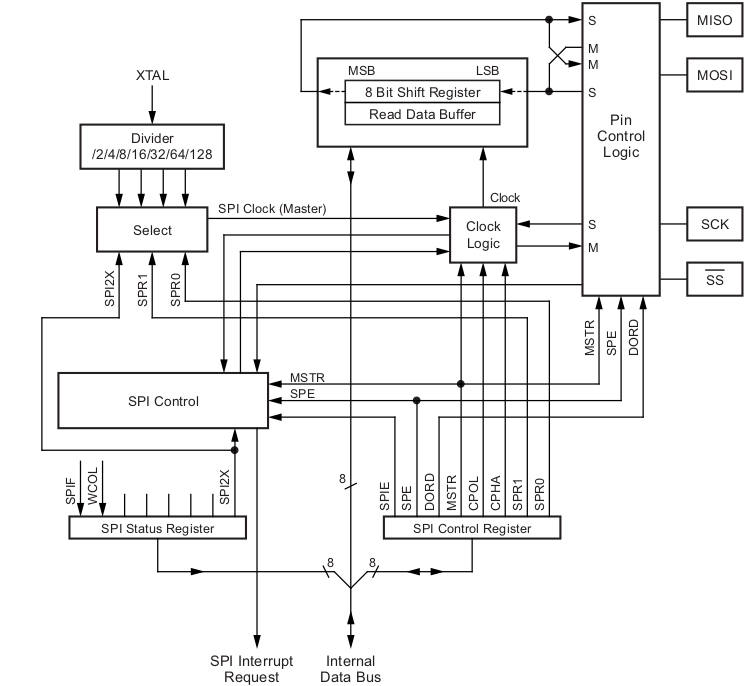
\includegraphics[height=0.6\textheight]{SPIBlockDiagram.png}
\end{figure}

\section{SPI Master-Slave Interconnection}
\begin{figure}[H]
    \centering
    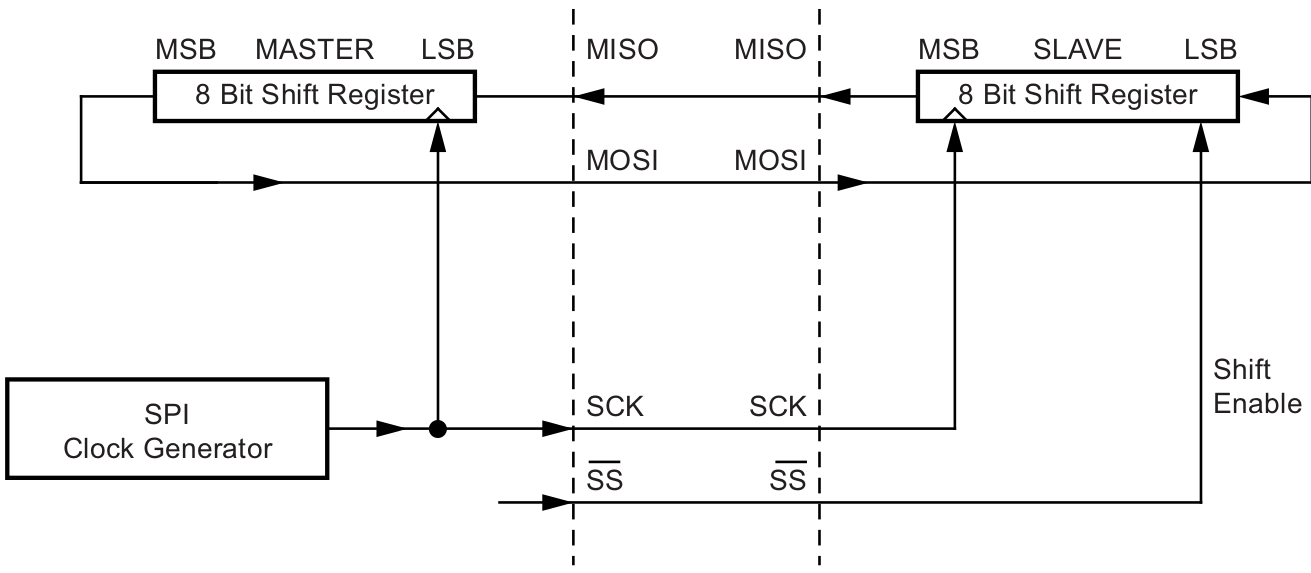
\includegraphics[width=0.6\textwidth]{SPIInterconnection.png}
\end{figure}
\subsection{SPI Pins}
\quad The SPI is connected to external devices trhough four pins namely,
\begin{itemize}
	\item \textbf{MISO} - Master IN / Slave OUT data - transmit data in slave mode and receive data in master mode.
	\item \textbf{MOSI} - Master OUT / Slave IN data - transmit data in master mode and receive data in slave mode.
	\item \textbf{SCK} - Serial Clock - outputs clock on SPI master mode and inputs clock on SPI slave mode.
	\item \textbf{NSS} - Slave Select - select the chip or the slave.
\end{itemize}
\subsection{Basic Operation}
\begin{itemize}
    \item Two shift Registers and a master clock generator.
    \item Initialization is done by pulling low the \pinFormat{$\overline{SS}$} pin.
    \item Master generates the required clock pulses on \pinFormat{SCK} to interchange data.
    \item Using \pinFormat{MOSI} – Master Out Slave In – data is shifted from master to slave.
    \item Using \pinFormat{MISO} – Master In Slave Out – data is shifted from slave to master.
    \item After each data packet, the master will synchronize the Slave by pulling high the Slave select  \pinFormat{$\overline{SS}$} pin.
\end{itemize}




\subsection{Clock Phase and Clock polarity}

\begin{itemize}
	\item \bitFormat{CPOL} bit controls the steady state value of \pinFormat{SCK} line when idle(no data is transferred).
	\begin{itemize}
		\item \bitFormat{CPOL} = 1 : \pinFormat{SCK} line is high-level idle state
		\begin{center}
			\begin{tikztimingtable}[%
				timing/dslope=0.1,
				timing/.style={x=5ex,y=2ex},
				x=5ex,
				timing/rowdist=3ex,
				timing/name/.style={font=\sffamily\scriptsize}
				]
				\busref{STATE} & 2D{IDLE} 5D{TRANSMISSION} 2D{IDLE};\\
				\busref{SCK}         & 4{h} 10{c} 4{h}\\				
			\end{tikztimingtable}
		\end{center}
			
		\item \bitFormat{CPOL}  = 0 : \pinFormat{SCK} line is low-level idle state
		\begin{center}
			\begin{tikztimingtable}[%
				timing/dslope=0.1,
				timing/.style={x=5ex,y=2ex},
				x=5ex,
				timing/rowdist=3ex,
				timing/name/.style={font=\sffamily\scriptsize}
				]
				\busref{STATE} & 2D{IDLE} 5D{TRANSMISSION} 2D{IDLE};\\
				\busref{SCK}         & 4{l} 10{c} 4{l}\\				
			\end{tikztimingtable}
		\end{center}
	\end{itemize}

	\item \bitFormat{CPHA} bit controls the capture of datas.
	\begin{itemize}
		\item \bitFormat{CPHA} = 1 : MSB bit is captured on the \textbf{second edge} of \pinFormat{SCK} pin (falling edge if the
		\bitFormat{CPOL} bit is 0, rising edge if the \bitFormat{CPOL} bit is 1).
		\begin{center}
			\begin{tikztimingtable}[%
				timing/dslope=0.1,
				timing/.style={x=5ex,y=2ex},
				x=5ex,
				timing/rowdist=3ex,
				timing/c/falling arrows,
				timing/name/.style={font=\sffamily\scriptsize}
				]
				\busref{STATE} & D{IDLE} 6D{TRANSMISSION} 2D{IDLE};\\
				\busref{SCK (CPOL=0)}         & 2{l} 12{c} 4{l}\\			
				\busref{MOSI} & 2D{MSB bit} D{} D{}; [dotted] D{}; D{} D{LSB bit} 2D{}\\		
				\busref{MISO} & 2D{MSB bit} D{} D{}; [dotted] D{}; D{} D{LSB bit} 2D{}\\	
				\extracode		
				\begin{pgfonlayer}{background}
					\begin{scope}[semitransparent,semithick]
						\vertlines[red]{1.5,2.5,...,7}
					\end{scope}	
				\end{pgfonlayer}
			\end{tikztimingtable}		
		\begin{tikztimingtable}[%
			timing/dslope=0.1,
			timing/.style={x=5ex,y=2ex},
			x=5ex,
			timing/rowdist=3ex,
			timing/c/rising arrows,
			timing/name/.style={font=\sffamily\scriptsize}
			]
			\busref{STATE} & D{IDLE} 6D{TRANSMISSION} 2D{IDLE};\\
			\busref{SCK (CPOL=1)}         & 2{h} 12{c} 4{h}\\			
			\busref{MOSI} & 2D{MSB bit} D{} D{}; [dotted] D{}; D{} D{LSB bit} 2D{}\\		
			\busref{MISO} & 2D{MSB bit} D{} D{}; [dotted] D{}; D{} D{LSB bit} 2.D{}\\	
			\extracode		
			\begin{pgfonlayer}{background}
				\begin{scope}[semitransparent,semithick]
					\vertlines[blue]{1.5,2.5,...,7}
				\end{scope}	
			\end{pgfonlayer}
		\end{tikztimingtable}
		
		\end{center}
		\item \bitFormat{CPHA} = 0 : MSB bit is captured on the \textbf{first edge} of \pinFormat{SCK} pin (falling edge if the
		\bitFormat{CPOL} bit is 1, rising edge if the \bitFormat{CPOL} bit is 0).
		\begin{center}
			\begin{tikztimingtable}[%
				timing/dslope=0.1,
				timing/.style={x=5ex,y=2ex},
				x=5ex,
				timing/rowdist=3ex,
				timing/c/rising arrows,
				timing/name/.style={font=\sffamily\scriptsize}
				]
				\busref{STATE} & D{IDLE} 6D{TRANSMISSION} 2D{IDLE};\\
				\busref{SCK (CPOL=0)}         & 2{l} 12{c} 4{l}\\			
				\busref{MOSI} & 1.5D{MSB bit} D{} D{}; [dotted] D{}; D{} D{LSB bit} 2.5D{}\\		
				\busref{MISO} & 1.5D{MSB bit} D{} D{}; [dotted] D{}; D{} D{LSB bit} 2.5D{}\\	
				\extracode		
				\begin{pgfonlayer}{background}
					\begin{scope}[semitransparent,semithick]
						\vertlines[blue]{1,2,...,6}
					\end{scope}	
				\end{pgfonlayer}
			\end{tikztimingtable}		
			\begin{tikztimingtable}[%
				timing/dslope=0.1,
				timing/.style={x=5ex,y=2ex},
				x=5ex,
				timing/rowdist=3ex,
				timing/c/falling arrows,
				timing/name/.style={font=\sffamily\scriptsize}
				]
				\busref{STATE} & D{IDLE} 6D{TRANSMISSION} 2D{IDLE};\\
				\busref{SCK (CPOL=1)}         & 2{h} 12{c} 4{h}\\			
				\busref{MOSI} & 1.5D{MSB bit} D{} D{}; [dotted] D{}; D{} D{LSB bit} 2.5D{}\\		
				\busref{MISO} & 1.5D{MSB bit} D{} D{}; [dotted] D{}; D{} D{LSB bit} 2.5D{}\\	
				\extracode		
				\begin{pgfonlayer}{background}
					\begin{scope}[semitransparent,semithick]
						\vertlines[red]{1,2,...,6}
					\end{scope}	
				\end{pgfonlayer}
			\end{tikztimingtable}
			
		\end{center}
	\end{itemize}
\end{itemize}

\subsection{Data Frame Format}
\quad The data can be shifted out either MSB first or LSB first.


\section{Register Description}
\subsubsection*{SPCR – SPI Control Register}
\vspace*{0.5cm}
\begin{bytefield}[bitformatting={\large\bfseries},
    endianness=big,bitwidth=0.125\linewidth]{8}
    \bitheader[lsb=0]{0-7} \\
    \bitbox{1}{\small SPIE}
    \bitbox{1}{\small SPE}
    \bitbox{1}{\small DORD}
    \bitbox{1}{\small MSTR}
    \bitbox{1}{\small CPOL}
    \bitbox{1}{\small CPHA}
    \bitbox{1}{\small SPR1}
    \bitbox{1}{\small SPR0}\\
\end{bytefield}

\begin{itemize}
    \item \bitFormat{SPIE - SPI Interrupt Enable} - Enable the SPI interrupt to be executed if \bitFormat{SPIF} bit is set in \regFormat{SPSR} Register.
    \item \bitFormat{SPE - SPI Enable} - Enable the SPI.
    \item \bitFormat{DORD - Data Order} - Defines the data order being sent[1 == LSB first; 0 == MSB first]
    \item \bitFormat{MSTR - Master/Slave Select} - Select between Master Mode and Slave Mode[1 == Master Mode; 0 == Slave Mode]
\end{itemize}

\begin{table}[H]
    \begin{center}
        \begin{tabular}{c|c}
            \bitFormat{SI2X, SPR1, SSPR0} & \textbf{SCK Frequency}\\
            \hline
            000 & $\frac{f_{OSC}}{4}$\\
            001 & $\frac{f_{OSC}}{16}$\\
            010 & $\frac{f_{OSC}}{64}$\\
            011 & $\frac{f_{OSC}}{128}$\\
            100 & $\frac{f_{OSC}}{2}$\\
            101 & $\frac{f_{OSC}}{8}$\\
            110 & $\frac{f_{OSC}}{32}$\\
            111 & $\frac{f_{OSC}}{64}$\\            
        \end{tabular}
    \end{center}
\end{table}


\subsubsection*{SPSR – SPI Status Register}
\vspace*{0.5cm}
\begin{bytefield}[bitformatting={\large\bfseries},
    endianness=big,bitwidth=0.125\linewidth]{8}
    \bitheader[lsb=0]{0-7} \\
    \bitbox{1}{\small SPIF}
    \bitbox{1}{\small WCOL}
    \bitbox{1}{\small -}
    \bitbox{1}{\small -}
    \bitbox{1}{\small -}
    \bitbox{1}{\small -}
    \bitbox{1}{\small -}
    \bitbox{1}{\small SPI2X}\\
\end{bytefield}
\begin{itemize}
    \item \bitFormat{SPIF - SPI Interrupt Flag} - Denotes the end of serial transfter. A intterup its generated if \bitFormat{SPIE} bit in \regFormat{SPCR} register is set.
\end{itemize}

\subsubsection*{SPDR – SPI Data Register}
\vspace*{0.5cm}
\begin{bytefield}[bitformatting={\large\bfseries},
    endianness=big,bitwidth=0.125\linewidth]{8}
    \bitheader[lsb=0]{0-7} \\
    \bitbox{1}{\small D7}
    \bitbox{1}{\small D6}
    \bitbox{1}{\small D5}
    \bitbox{1}{\small D4}
    \bitbox{1}{\small D3}
    \bitbox{1}{\small D2}
    \bitbox{1}{\small D1}
    \bitbox{1}{\small D0}\\
\end{bytefield}

\section{Configuring the SPI}
\begin{itemize}
    \item First, the pins \pinFormat{MOSI}, \pinFormat{MISO}, \pinFormat{SCK} and \pinFormat{$\overline{SS}$} is configured to required Direction.
    \item Next, the \pinFormat{$\overline{SS}$}  pin is made low or high depending on the device Specs.
    \item The data order is selected by \bitFormat{DORD} bit in \regFormat{SPCR} register.
    \item The Master/Slave Mode is selected by \bitFormat{MSTR} bit in \regFormat{SPCR} register.
    \item The timing is choosen by Configuring \bitFormat{CPOL} and \bitFormat{CPHL} bit in \regFormat{SPCR} register depending on the Device Specs.
    \item The Clock Frequency for SPI communication is choosen by Configuring the \bitFormat{SPI2X}, \bitFormat{SPR1} and \bitFormat{SPR} bits of \regFormat{SPCR} and \regFormat{SPSR} registers.
    \item Interrupt is enabled by setting the \bitFormat{SPIE} bit in \regFormat{SPCR} register.
    \item FInally, SPI is enabled by setting the \regFormat{SPE} bit in \regFormat{SPCR} register.
    \item Also, the interrupt service routing is written, when the transmission/reception completes.
    \item The data can be transmitted/received by writing/reading from \regFormat{SPIDR} register.
    \item An example code is seen below,
\end{itemize}

\begin{minted}[breaklines, bgcolor=lightgray]{c}
// making SCK, MOSI, SS' as outptut
DDRB |= (1<<DDB2) | (1<<DDB3) | (1<<DDB5);
// making MISO as input
DDRB &= ~(1<<DDB4);

// making SCK, MOSI,  as low
PORTB &=  ~(1<<PORTB3) & ~(1<<PORTB5);
// making SS' as high
PORTB |= (1<<PORTB2);

// Select MSB first or LSB first by DORD
SPCR &= ~(1<<DORD);
	
// Select this as Master
SPCR |= (1<<MSTR);

// Let the clock polarity be SCK is low when idle
SPCR &= ~(1<<CPOL);

// Sampled at Rising or Falling Edge
// we choose rising edge
SPCR &= ~(1<<CPHA);

// Selecting a SCK frequnecy
// we select Fosc/4 by 000
SPSR &= ~(1<<SPI2X);
SPCR &= ~(1<<SPR1);
SPCR &= ~(1<<SPR0);
// dISBALE SPIE bit for interrupt on Serial Transfer Completion
SPCR &= ~(1<<SPIE);
// Enabling SPI
SPCR |= (1<<SPE);
\end{minted}

\begin{minted}[breaklines, bgcolor=lightgray]{c}
uint8_t SPITransferReceive(uint8_t data_)
{
    SPDR = data_;
    // wait till serial transmission is complete by checking the SPI Interrupt Flag
    while((SPSR & (1<<SPIF)) == 0 ) {};
    // return the recieved data - can use it or ignore it
    return SPDR;
}
\end{minted}
\end{document}

\chapter{Universal Synchronous and Asynchronous serial Receiver and Transmitter 0}
\documentclass{article}

\usepackage[a4paper, bottom=0.5in, top=0.5in, left=0.5in, right=0.5in]{geometry}
\usepackage{wrapfig}
\usepackage{natbib}
\usepackage{url}
\usepackage{xcolor}
\usepackage{caption}
\usepackage{hyperref}
\hypersetup{
    colorlinks=true,    
    urlcolor=cyan,
}
\usepackage{bytefield}

\usepackage{amsfonts}
\usepackage{float}
\usepackage{enumitem}

\usepackage{tikz-timing}[2014/10/29]
\usetikztiminglibrary[rising arrows]{clockarrows}

\usepackage{minted}

\usepackage{xparse} % NewDocumentCommand, IfValueTF, IFBooleanTF
\usepackage{tikz-timing}[2014/10/29]
\NewDocumentCommand{\busref}{som}{\texttt{%
		#3%
		\IfValueTF{#2}{[#2]}{}%
		\IfBooleanTF{#1}{\#}{}%
}}


\newcommand{\bitFormat}[1]{\emph{\textbf{\textcolor{cyan}{#1}}}}

\newcommand{\regFormat}[1]{\textbf{\textcolor{magenta}{#1}}}

\newcommand{\pinFormat}[1]{\emph{\textcolor{red}{#1}}}


\usepackage{graphicx}
\graphicspath{ {./Resources/pics/} }



\title{ATmega328P USART0}
\author{Narendiran S}
\date{\today}

\begin{document}
\maketitle

\section{Features}
\begin{itemize}
    \item Full duplex operation (independent serial receive and transmit registers).
    \item Asynchronous or synchronous operation
    \item High resolution baud rate generator
    \item Serial frame with 5,6,7,8,9 data bits and 1 or 2 stop bits
    \item Odd or even partiy generator and checker by hardware
    \item Double speed asynchronous communication mode
\end{itemize}
\section{Block Diagram}
\begin{figure}[H]
    \centering
    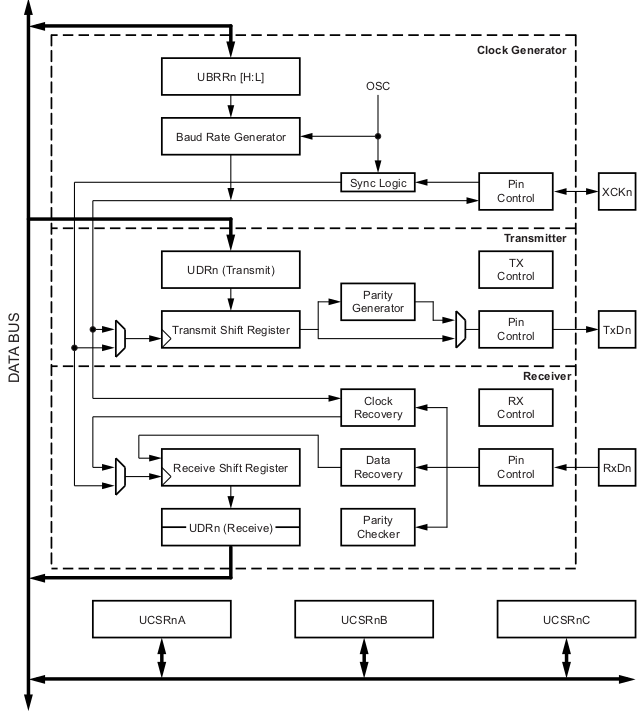
\includegraphics[height=0.58\textheight]{USART0BlockDiagram.png}
\end{figure}

\subsection{Clock Generator Block}
\begin{itemize}
    \item Consist of sync. Logic for external clock input for usage in sync. slave operation 
    \item Consist of Baud rate Generator.
    \item Uses the \pinFormat{XCKn} pin for sync. Transfer mode
\end{itemize}

\subsection{Transmitte Block}
\begin{itemize}
    \item Consist of singe write buffer – continuous transfer of data without delay between frames
    \item Consist of Serial Shift register and Parity Generator
    \item Also, Control logic for handling different serial frame format.
\end{itemize}

\subsection{Receiver Block}
\begin{itemize}
    \item Consist of Clock and data recovery unit – uses for Asynchronous reception
    \item Consist of Parity Checker, Control Logic, Shift Register, Two level Receiver buffer
    \item Can support frame error, data overrun parity error
\end{itemize}

\section{Clock Genration}
\begin{figure}[H]
    \centering
    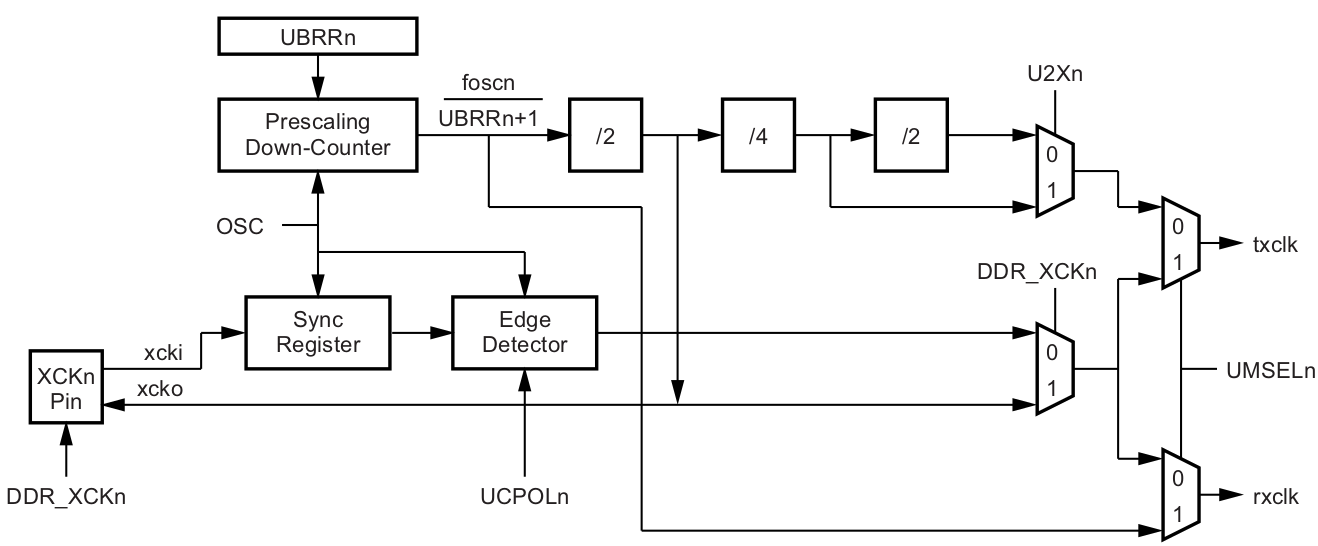
\includegraphics[width=1\textwidth]{USART0ClockGeneration.png}
\end{figure}
\begin{itemize}
    \item Generates Base Clock for Transmitter and Receiver.
    \item USART supports four modes of clock operation
    \begin{enumerate}[label=(\roman*)]
        \item Normal Asynchronous
        \item Double Speed Asynchronous
        \item Master synchronous
        \item Slave synchronous
    \end{enumerate}
    \item Selection between Asynchronous and Synchronous is done by \bitFormat{UMSELn} bit in \bitFormat{UCSRnC} - USART Control and Status Register C.
    \item The Double Speed is selected by \bitFormat{U2Xn} bit in \bitFormat{UCSRnA} - USART Control and Status Register A.
    \item In Synchronous Mode, the master or slave mode is selected by \bitFormat{DDR\_XSCn} bit direction. [external - slave mode; internal - master mode]
\end{itemize}
\begin{table}[H]
    \begin{center}
        \begin{tabular}{c|c}
            \textbf{Signals} & \textbf{Description}\\
            \hline
            txclk & Transmitte Clock\\
            rxclk & Receiver Base Clock\\
            xclki & Input from \pinFormat{XCK} pin - used for synchronous slave operation.\\
            xclko & Clock output to \pinFormat{XCK} pin - used for synchronous master operation.\\
            fosc & \pinFormat{XTAL} pin freqency (System clock).
        \end{tabular}
    \end{center}
\end{table}

\subsection{Internal Clock Generation - The Baud Rate Generator}
\begin{itemize}
    \item Used for Asynchronous and Synchronous Master modes of operation.
    \item Programmed using \regFormat{UBRRn} register.
\end{itemize}

\begin{table}[H]
    \begin{center}
        \begin{tabular}{c|c}
            \textbf{Operating Mode} & \textbf{UBRRn calculation}\\
            \hline
            Asynchronous Normal Mode(\bitFormat{U2Xn} == 0) & $UBRRn = \frac{f_{OSC}}{16 * BAUD} - 1$\\
            Asynchronous Double Speed Mode(\bitFormat{U2Xn} == 1) & $UBRRn = \frac{f_{OSC}}{8 * BAUD} - 1$\\
            Synchronous Master Mode & $UBRRn = \frac{f_{OSC}}{2 * BAUD} - 1$\\
        \end{tabular}
    \end{center}
\end{table}

\subsection{External Clock}
\begin{itemize}
    \item Used by synchronous Slave mode.
    \item External clock input from \pinFormat{XCKn} pin is used and should
\end{itemize}
\begin{center}
    $f_{XCK} < \frac{f_{OSC}}{4}$
\end{center}

\section{Frame Format}
\begin{figure}[H]
    \centering
    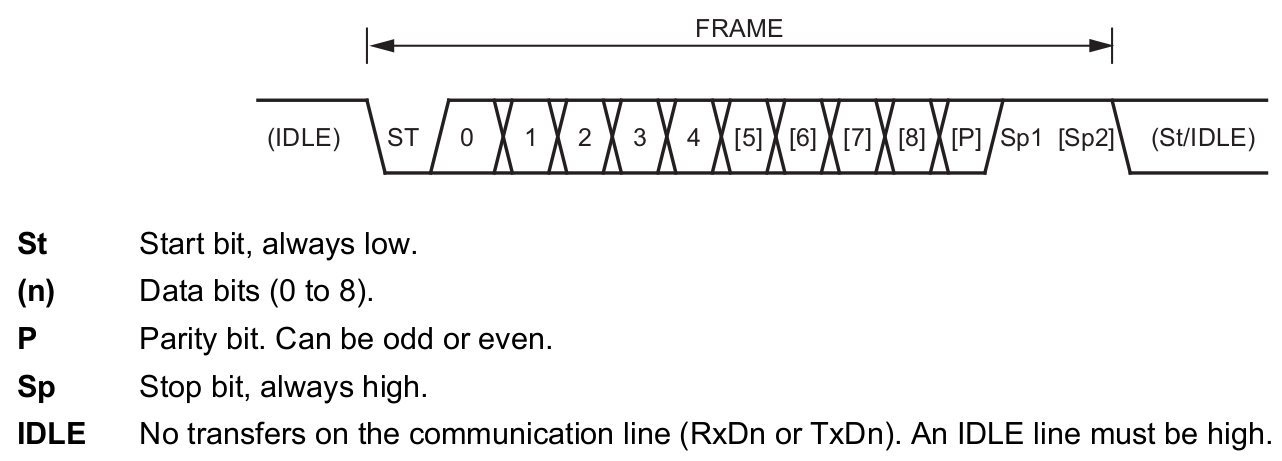
\includegraphics[width=1\textwidth]{USART0FrameFormat.png}
\end{figure}
\begin{itemize}
    \item A serial frame is defined to be one character of data bits with synchronization bits (start and stop bits), and optionally a parity bit for error checking.
    \item The combinations can be
    \begin{itemize}
        \item 1 start bit
        \item 5 or 6 or 7 or 8 or 9 data bits
        \item no or even or odd parity bits
        \item 1 or 2 stop bits
    \end{itemize}
    \item A frame starts with start bit followed by LSB data bits.
    \item Next the data bet can be from 5 to 9 ending with MSB data bits.
    \item Parity bits may be added if enabled.
    \item Finally, stop bit of 1 or 2 size is added.
    \item Generally, the line is idel with high Logic.
\end{itemize}
\section{Register Description}
\subsection*{UDRn – USART I/O Data Register n}
\vspace*{0.5cm}
\begin{bytefield}[bitformatting={\large\bfseries},
    endianness=big,bitwidth=0.125\linewidth]{8}
    \bitheader[lsb=0]{0-7} \\
    \bitbox{8}{\small RXB[7:0]}\\
    \bitbox{8}{\small TXB[7:0]}\\
\end{bytefield}

\subsubsection*{UCSRnA – USART Control and Status Register n A}
\vspace*{0.5cm}
\begin{bytefield}[bitformatting={\large\bfseries},
    endianness=big,bitwidth=0.125\linewidth]{8}
    \bitheader[lsb=0]{0-7} \\
    \bitbox{1}{\small RXCn}
    \bitbox{1}{\small TXCn}
    \bitbox{1}{\small UDREn}
    \bitbox{1}{\small FEn}
    \bitbox{1}{\small DORn}
    \bitbox{1}{\small UPEn}
    \bitbox{1}{\small U2Xn}
    \bitbox{1}{\small MPCMn}\\
\end{bytefield}
\subsubsection*{UCSRnB – USART Control and Status Register n B}
\vspace*{0.5cm}
\begin{bytefield}[bitformatting={\large\bfseries},
    endianness=big,bitwidth=0.125\linewidth]{8}
    \bitheader[lsb=0]{0-7} \\
    \bitbox{1}{\small RXCIEn}
    \bitbox{1}{\small TXCIEn}
    \bitbox{1}{\small UDRIEn}
    \bitbox{1}{\small RXENn}
    \bitbox{1}{\small TXENn}
    \bitbox{1}{\small UCSZn2}
    \bitbox{1}{\small RXBn}
    \bitbox{1}{\small TXB8n}\\
\end{bytefield}
\subsubsection*{UCSRnC – USART Control and Status Register n C}
\vspace*{0.5cm}
\begin{bytefield}[bitformatting={\large\bfseries},
    endianness=big,bitwidth=0.125\linewidth]{8}
    \bitheader[lsb=0]{0-7} \\
    \bitbox{1}{\small UMSELn1}
    \bitbox{1}{\small UMSELn0}
    \bitbox{1}{\small UPMn1}
    \bitbox{1}{\small UPMn0}
    \bitbox{1}{\small USBSn}
    \bitbox{1}{\small UCSZn1}
    \bitbox{1}{\small UCSZn0}
    \bitbox{1}{\small UCPOLn}\\
\end{bytefield}


\begin{itemize}
    \item \bitFormat{RXCn} - USART Receive Complete - Set when there are unread data in receive buffer.
    \item \bitFormat{TXCn} - USART Transmit Complete - Set when the entire frame in the transmit shift register has been shifted out and there are no new data currently present in the transmit buffer.
    \item \bitFormat{UDREn} - USART Data Register Empty - indicates if the transmit buffer is ready to receive new data. A one indicates buffer is expty and ready to transmit.
    \item \bitFormat{U2Xn} - Double the USART Transmission Speed - Affects only the asynchronous operation. One will increase the speeed of transfer rate in asynchronous opration.
    \item \bitFormat{RXCIEn} - RX Complete Interrupt Enable n - Writing one will enabled Receive Complete intterrupt.
    \item \bitFormat{TXCIEn} - TX Complete Interrupt Enable n - Writing one will enabled Transmit Complete intterrupt.
    \item \bitFormat{UDRIen} - USART Data Register Empty Interrupt Enable n - Enable data register empty intterrupt.
    \item \bitFormat{RXENn} - Receiver Enable - enable the receiever for reception.
    \item \bitFormat{TXENn} - Transmitter Enable - enable the Transmitter for Transmission.
    \item \bitFormat{UCSZn[2:0]} - Character Size n - select the number of data bits in a frame.
    \item \bitFormat{RXB8n} - Receive Data Bit 8 n - it's the actual 9th bit received.
    \item \bitFormat{TXB8n} - Transmit Data Bit 8 n -  it's the actual 9th bit to tbe trasnmitted.
    \item \bitFormat{UMSELn[1:0]} - USART Mode Select - Select the mode.
    \item \bitFormat{UPMn[1:0]} - Parity Mode - Disable or set the parity mode type.
    \item \bitFormat{USBSn} - Stop Bit select - Selects the number of stop bits to be inserted by transmitter.
\end{itemize}

\begin{table}[H]    
\begin{minipage}{0.4\linewidth}
    \begin{tabular}{c|c}
        \bitFormat{UMSELn[1:0]} & \textbf{Mode}\\
        \hline
        00 & Asynchronous USART\\
        01 & Synchronous USART\\
        10 & Reserved\\
        11 & Master SPI\\
    \end{tabular}
\end{minipage}
\begin{minipage}{0.3\linewidth}
    \begin{tabular}{c|c}
        \bitFormat{UPMn[1:0]} & \textbf{Parity Mode}\\
        \hline
        00 & Disabled\\
        01 & Reserved\\
        10 & Even Parity\\
        11 & Odd Parity\\
    \end{tabular}
\end{minipage}
\begin{minipage}{0.29\linewidth}
    \begin{tabular}{c|c}
        \bitFormat{USBSn} & \textbf{Stop Bit(s)}\\
        \hline
        0 & 1-bit\\
        0 & 2-bit\\
    \end{tabular}
\end{minipage}
\end{table}

\begin{table}[H]
    \begin{center}
        \begin{tabular}{c|c}
            \bitFormat{UCSZn[2:0]} & \textbf{Character Size}\\
            000 & 5-bit\\
            001 & 6-bit\\
            010 & 7-bit\\
            011 & 8-bit\\
            111 & 9-bit\\
        \end{tabular}
    \end{center}
\end{table}

\subsubsection*{UBRRnL and UBRRnH – USART Baud Rate Registers}
\vspace*{0.5cm}
\begin{bytefield}[bitformatting={\large\bfseries},
    endianness=big,bitwidth=0.125\linewidth]{8}
    \bitheader[lsb=8]{8-15} \\
    \bitbox{1}{\small -}
    \bitbox{1}{\small -}
    \bitbox{1}{\small -}
    \bitbox{1}{\small -}
    \bitbox{4}{\small UBRRn[11:8}\\
    \bitbox{8}{\small UBRRn[7:0}\\\\    
    \bitheader[lsb=0]{0-7} \\
\end{bytefield}

\quad \bitFormat{UBRRn[11:0]} - the actual 12-bit USART Baud Rate Registers.

\section{Configurint USART}
\begin{itemize}
    \item First, the mode is selected by confguring the \bitFormat{UMSEL0[1:0]} bits in \regFormat{UCSR0C} register.
    \item Next, the Baud rate is choosen and set in \bitFormat{UBRR0[11:0]} bits in \regFormat{UBRR0H} and \regFormat{UBRR0L} registers.
    \item Next, the frame format is set by confguring,
    \begin{itemize}
        \item Data Length - by confguring \bitFormat{UCSZ0[2:0]} bit  in \regFormat{UCSR0B} and \regFormat{UCSR0C} register.
        \item Parity - by confguring \bitFormat{UPM0[1:0]} bit  in \regFormat{UCSR0C} register.
        \item Stop bits - by confguring \bitFormat{USBS0} bit  in \regFormat{UCSR0C} register.
    \end{itemize}
    \item Interrupt may be anabled by setting bits in \bitFormat{UCSR0A} register and ISR are wirtten.
    \item Finally, the Transmitter and Receiver are enabled by setting \bitFormat{TXEN0} and \bitFormat{RXEN0} bits in \regFormat{UCSR0B}.
    \item The data can be sent by checking if the \bitFormat{UDRE0} bit is set in \regFormat{UCSR0A} register and wiring the 8-bit data into \regFormat{UDR0} register.
    \item The data can be received by checking if the \bitFormat{RXC0} bit is set in \regFormat{UCSR0A} register and reading the 8-bit data from \regFormat{UDR0} register.
    \item The code for a simple USART is seen below,
\end{itemize}

\begin{minted}[breaklines, bgcolor=lightgray]{c}
// Setting up the Mode
// Select the Asyncronous Master Mode.
// Setting UMSEL0[1:0] in UCSR0C to 00
UCSR0C &= ~(1<<UMSEL00);
UCSR0C &= ~(1<<UMSEL01);

// setting up the Buad rate
// Due to The Clock rate being 8MHz, for a buad rate of 9600
// UBRR0 = (fosc / (16*BAUD)) -1
// So UBRR0 = (8000000 / (16 * 9600)) - 1 = 0x33
UBRR0H = 0x00;
UBRR0L = 0x33;

// setting up the Frame Format
// Let's select 8-bit data bits, no parity, and 1 stop bit
// 8 - bit data bits
// By selecting UCSZ0[2:0] in UCSR0C and UCSR0B register to be 011
UCSR0B &= ~(1<<UCSZ02);
UCSR0C |= (1<<UCSZ01);
UCSR0C |= (1<<UCSZ00);
// No parity
// By selecting UPM0[1:0] in UCSR0C to 00
UCSR0C &= ~(1<<UPM01);
UCSR0C &= ~(1<<UPM00);
// 1 stop bit
// By selecting USBS0 in UCSR0C to 0 
UCSR0C &= ~(1<<USBS0);

// Disabling any interrupts
UCSR0B &= ~(1<<7);
UCSR0B &= ~(1<<6);
UCSR0B &= ~(1<<5);

// Enabling Transmitter 
UCSR0B |= (1<<TXEN0);
// Enabling Receiver
UCSR0B |= (1<<RXEN0);
\end{minted}

\begin{minted}[breaklines, bgcolor=lightgray]{c}
void USART0sendChar(uint8_t data_)
{
	//cHECKING if transmitet buffer is empty
	while((UCSR0A & (1<<UDRE0)) == 0x00){};		
	UDR0 = data_;	
}
uint8_t USART0receiveChar()
{
	// wait for thedate to be recied
	while((UCSR0A & (1<<RXC0)) == 0x00){};		
	return UDR0;
}
\end{minted}

\end{document}

\chapter{Two Wire Interface}
\documentclass{article}
\usepackage{NeededPackages}



\begin{document}


\section{Features}
\begin{itemize}
    \item 7-bit address space allows up to 128 different slave addresses
    \item Multi-master arbitration support
    \item Up to 400kHz data transfer speed
    \item Noise suppression circuitry rejects spikes on bus lines
    \item Fully programmable slave address with general call support
    \item Compatible with Phillips I­2C
\end{itemize}
\section{2-wire Serial Interface}
\begin{itemize}
    \item Suited for typical microcontroller applications
    \item Allows upto  128 different device.
    \item All devices connected must have individual address and method to resolved bus contention
\end{itemize}

\subsection{\texorpdfstring{$I^2C$}{} Pins}
\begin{itemize}
    \item Output driver consist of slew-rate limiter to confirm the TWI specification.
    \item Input stage consist of spike suppression unit to remove spikes shorter than 50ns.
    \item Internal pull-up can also be used.
    \item \pinFormat{SDA} - Serial Data - the actual serial data transfer pinFormat
    \item \pinFormat{SCL} - Serial Clock - driven by device in Master Mode
\end{itemize}

\subsection{Terminology}
\begin{table}[H]
    \begin{center}
        \begin{tabular}{c|c}
            \textbf{Term} & \textbf{Descripton}\\
            \hline
            Master & Device that initiates and terminates transacting and also Generates \pinFormat{SCL} Clock.\\
            Slave & Device addressed by a master.\\
            Transmitter & Device placing data on the bus.\\
            Receiver & Device reading data on the bus.\\
        \end{tabular}
    \end{center}
\end{table}

\subsection{Electrical Interconnection}
\begin{figure}[H]
    \centering
    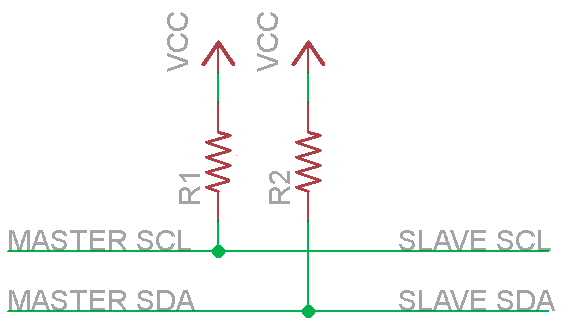
\includegraphics[width=0.3\textwidth]{i2cElectrical.png}
\end{figure}
\begin{itemize}
    \item both lines are connected to positive supply voltage through pull-up resistor
    \item bus driver are open-drain or open-collector
    \item no. of device also depends on the bus capacitance limit of 400pF
\end{itemize}

\section{Data Transfer and Frame Format}

\subsection{Transferring Bits}
\begin{figure}[H]
    \centering
    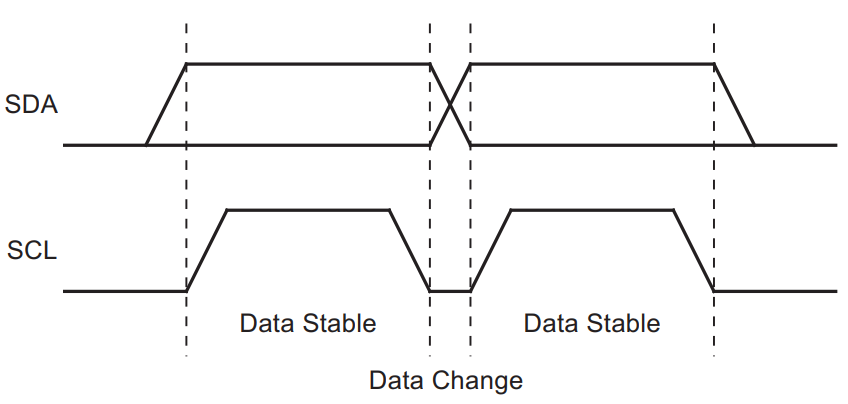
\includegraphics[width=0.5\textwidth]{i2cTransferBits.png}
\end{figure}
\begin{itemize}
    \item Each data bit transferred is done by a pulse on clock line.
    \item Level of data line must be stable when the clock line is high.
\end{itemize}

\subsection{START and STOP Conditions}
\begin{figure}[H]
    \centering
    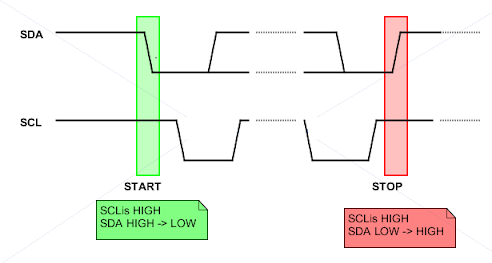
\includegraphics[width=0.7\textwidth]{i2cSTARTSTOP.png}
\end{figure}
\begin{itemize}
	\item Both \iicFormat{START} and \iicFormat{STOP} conditions are done by changing \pinFormat{SDA} line when \pinFormat{SCL} is kept high.
	\item Master initiates transmission by issuing a \iicFormat{START} condition.
	\item Master terminates transmission by issuing a \iicFormat{STOP} condition.
	\item Between \iicFormat{START} and \iicFormat{STOP}, bus is busy and no other master should try to control bus.
	\item The same master however can issue \iicFormat{REPEATED START}(same as \iicFormat{START}) to initiate a new transfer.
\end{itemize}

\subsection{Address Packet format}
    \begin{figure}[H]
        \begin{center}
            \includegraphics[width=0.8\textwidth]{i2cAddressPacketFormat}
        \end{center}
    \end{figure}
\begin{itemize}
	\item Addresses packets(\iicFormat{SLA}) are 9-bit long.
	\begin{itemize}
		\item 7 address bits with MSB transmitted first
		\item one READ(1)/WRITE(0) control bit indicating the transmitter or receiver mode respectively
		\item one acknowledge bit by the Slave	
	\end{itemize}	
	\item Would take 8 clock cycles by the master to send 7 address bits and one READ/WRITE control bit. \iicFormat{SLA+R} or \iicFormat{SLA+W}.
	\item On the 9th clock cycle, Master will leave out the control of \pinFormat{SDA} line (making it high due to pull-up resistor) but clocks out the 9th clock on the \pinFormat{SCL} line.
	\item On the 9th clock cycle, Slave recognizes that it is being addressed by pulling \pinFormat{SDA} line low making the \iicFormat{ACK}.
	\item If the Slave couldn’t for some reason respond, the \pinFormat{SDA} line remains high in the 9th clock cycle making the \iicFormat{NACK}.
\end{itemize}

\subsection{Data Packet format}
\begin{itemize}
	\item Data packetsare 9-bit long.
	\begin{itemize}
		\item one data byte - 8 bits with MSB first.
		\item one acknowledge bit by the master or slave depending the mode.
	\end{itemize}
	\item The transmitter(either the master or slave) send 8-bit data in 8 clock cycles.
	\begin{figure}[H]
		\begin{center}
			\includegraphics[width=0.8\textwidth]{i2cDataFrame}
		\end{center}
	\end{figure}
	\item On the 9th clock cycle, the transmitter will leave out the control of \pinFormat{SDA} line (making it high due to pull-up resistor).
	\item During the 9th clock cycle, the receiver pulls down the \pinFormat{SDA} line low to acknowledge the reception. – \iicFormat{ACK} is signaled by receiver.
	\item If the receiver doesn’t pull down the \pinFormat{SDA} line for some reason, then the \pinFormat{SDA} line remains high. – \iicFormat{NACK} is signaled by receiver.
	\item When the receiver received the last byte or can’t receive more byte, it should inform the transmitter by sending a \iicFormat{NACK}.
\end{itemize}
\subsection{Overall Operation}
\subsubsection*{Write Operation}
\begin{tikztimingtable}[%
    timing/dslope=0.1,
    timing/.style={x=5ex,y=2ex},
    x=5ex,
    timing/rowdist=3ex,
    timing/name/.style={font=\sffamily\scriptsize}
    ]
    \busref{SDA} & h l l l D{A6} D{A5} [dotted] D{}; D{A0} D{R}
    D{$\overline{ACK}$}
    D{D7} D{D6} [dotted] D{}; D{D0}
    D{$\overline{ACK}$}
    D{D7} D{D6} [dotted] D{}; D{D0}
    D{NACK}
    L l H
     \\
    \busref{SCL} & 0.75H l l l 15{h l} h l l l H 0.5h\\
\end{tikztimingtable}
\subsubsection*{Read Operation}
\begin{tikztimingtable}[%
    timing/dslope=0.1,
    timing/.style={x=5ex,y=2ex},
    x=5ex,
    timing/rowdist=3ex,
    timing/name/.style={font=\sffamily\scriptsize}
    ]
    \busref{SDA} & h l l l D{A6} D{A5} [dotted] D{}; D{A0} D{R}
    D{$\overline{ACK}$}
    D{D7} D{D6} [dotted] D{}; D{D0}
    D{$\overline{ACK}$}
    D{D7} D{D6} [dotted] D{}; D{D0}
    D{NACK}
    L l H
     \\
    \busref{SCL} & 0.75H l l l 15{h l} h l l l H 0.5h\\
\end{tikztimingtable}

\newpage

\section{TWI Module}
\subsection{Block Diagram}
\begin{figure}[H]
    \centering
    \includegraphics[width=1\textwidth]{TWIModuleOVerview.png}
\end{figure}
\subsection{Bit Rate Generation Unit}
\begin{itemize}
    \item controls \pinFormat{SCL} line when in Master mode
    \item \bitFormat{TWBR} (TWI Bit Rate Generator) and Prescalar Bits in TWI status register \regFormat{TWSR} control \pinFormat{SCL}
    \item The \pinFormat{SCL} frequency can be
\end{itemize}
\begin{center}
    $SCL frequency = \frac{CPU Clock Frequency}{16 + 2 * TWBR * Prescalar Value}$
\end{center}
\textbf{Note: } Slave’s clock frequency must be atleast 16 times higher than SCL frequency.

\subsection{Bus Interface Unit}
\begin{itemize}
    \item contains Data and adress Shift register - \regFormat{TWDR} register - address or data transmitted or received
    \item \iicFormat{START/STOP} Controller - Generates and detects \iicFormat{START}, \iicFormat{STOP} and \iicFormat{REPEATED START}
    \item Register Containing the \iicFormat{(N)ACK} to be transmitted or received
    \item Arbitration detection hardware.
\end{itemize}

\subsection{Address Match Unit}
\begin{itemize}
    \item Received address bytes matches the seven-bit address in \regFormat{TWAR} (TWI Address register).
    \item address match results in informing the control unit
\end{itemize}

\subsection{Control Unit}
\begin{itemize}
    \item Monitors TWI bus and generates responses based on TWI control register (\regFormat{TWCR}).
    \item When a en even requires attention:
    \begin{itemize}
        \item \bitFormat{TWINT} (TWI Interrupt flag ) is set 
        \item \regFormat{TWSR} (TWI Status Register) is updated with status code identifying the event.
        \item when the \bitFormat{TWINT} is set, the \pinFormat{SCL} line is held low.
    \end{itemize}
    \item \bitFormat{TWINT} flag is set If
    \begin{itemize}
        \item TWI has transmitted a \iicFormat{START/REPEATED START} condition
        \item TWI has transmitted \iicFormat{SLA+R/W}
        \item TWI has transmitted an address byte
        \item TWI has lost arbitration
        \item TWI has been addressed by own slave address or general call
        \item TWI has received a data bye
        \item \iicFormat{STOP} or \iicFormat{REPEATED START} has been received
        \item bus error occurred due to illegal \iicFormat{START} or \iicFormat{STOP}
    \end{itemize}
\end{itemize}

\section{TWI Usage}
\begin{itemize}
    \item TWI is interrupt based and so \bitFormat{TWIE} bit in \regFormat{TWCR} register should be enabled; If the \bitFormat{TWIE} is diabled, then the \bitFormat{TWINT} flag must be polled.
    \item When the \bitFormat{TWINT} flag is asserted, TWI has finised operation and awaits for application response and \regFormat{TWSR} register describes the current status of TWI bus.
    \item Then, application should respond by manipulating the \regFormat{TWCR} and \regFormat{TWDR} register.
\end{itemize}

\subsection{An Example - Master transmits single data byte to slave}
\begin{figure}[H]
    \centering
    \includegraphics[width=1\textwidth]{TWIExample.png}
\end{figure}
\begin{enumerate}
    \item Transmission is started by writing specific value into \regFormat{TWCR} register to transmit the \iicFormat{START} condition. The \bitFormat{TWINT} flag is cleared by writing Loging HIGH which initiate the transmission of \iicFormat{START} condition.
    \item When the \iicFormat{START} condition has been transmitted, the TWINT flag in TWCR is set, and \regFormat{TWSR} is updated with a status code indicating that the \iicFormat{START} condition has successfully been sent.
    \item The application should now respond by examining the \regFormat{TWSR} register value. If status code is as expected, the application loads \iicFormat{SLA+W} into \regFormat{TWDR} and a specific value is written into \regFormat{TWCR} register to transmit the \iicFormat{SLA+W} present in \regFormat{TWDR}. The \bitFormat{TWINT} flag is cleared by writing logic HIGH which initiates the transmission of address packet.
    \item When the address packet has been transmitted, the \bitFormat{TWINT} flag in \regFormat{TWCR} is set, and \regFormat{TWSR} is updated with a status code indicating that the address packet has successfully been sent. The status code will also reflect whether a slave acknowledged the packet or not.
    \item The application should now respond by examining the \regFormat{TWSR} register value and \iicFormat{ACK} bit is as expected. If status code is as expected, the application loads Data packet into \regFormat{TWDR} and a specific value is written into \regFormat{TWCR} register to transmit the Data packet present in \regFormat{TWDR}. The \bitFormat{TWINT} flag is cleared by writing logic HIGH which initiates the transmission of data packet.
    \item When the data packet has been transmitted, the \bitFormat{TWINT} flag in \regFormat{TWCR} is set, and \regFormat{TWSR} is updated with a status code indicating that the data packet has successfully been sent. The status code will also reflect whether a slave acknowledged the packet or not.
    \item The application should now respond by examining the \regFormat{TWSR} register value and \iicFormat{ACK} bit is as expected. If status code is as expected, the application loads a specific value is written into \regFormat{TWCR} register to transmit the \iicFormat{STOP} Condition. The \bitFormat{TWINT} flag is cleared by writing logic HIGH which initiates the transmission of STOP condition.
\end{enumerate}

\section{Transmission Modes}
\quad There are four major Modes
\begin{enumerate}[label=(\roman*)]
    \item Master Transmitter (MT)
    \item Master Receiver (MR)
    \item Slave Transmitter (ST)
    \item Slave Receiver (SR)
\end{enumerate}
\begin{table}[H]
    \begin{center}
        \begin{tabular}{c|c}
            \textbf{Status Code} & \textbf{Meaning}\\
            \hline
            S & \iicFormat{START} Condition\\
            Rs & \iicFormat{REPEATED START} Condition\\
            R & Read bit (high level on \pinFormat{SDA})\\
            W & Write bit (low level on \pinFormat{SDA})\\
            A & Acknowledge bit (low level on \pinFormat{SDA})\\
            $\overline{A}$ & Not Acknowledge bit (high level on \pinFormat{SDA})\\
            DATA & 8-bit data\\
            P & \iicFormat{STOP} Condition\\
            SLA & Slave Address\\
        \end{tabular}
    \end{center}
\end{table}


\subsection{Master Transmitter Mode (MT)}
\begin{itemize}
    \item Many number of data bytes are transmitted to Slave receiver.
    \item For Master, \iicFormat{START} Condition is transmitted
    \item \iicFormat{START} condition is sent by:
    \begin{itemize}
        \item \bitFormat{TWEN} bit is set to enable TWI.
        \item \bitFormat{TWSTA} bit is set to transmit \iicFormat{START} condition.
        \item \bitFormat{TWINT} flag is written 1 to clear to send start bit.
        \item After Tranmitting \iicFormat{START} condition, \bitFormat{TWINT} flag is set by hardware and status code in \regFormat{TWSR} register should be \statusCode{0x08} - indicating successfull transmission of \iicFormat{START} condition.
    \end{itemize}
    \item  To enter into Master Transmitter Mode and transmit the address:
    \begin{itemize}
        \item Write \iicFormat{SLA+W} into \regFormat{TWDR} register.
        \item \bitFormat{TWINT} flag is written 1 to clear to transmit Address and read/write status.
        \item After transmitting \iicFormat{SLA+W}, an acknowledgment bit will be received, the \bitFormat{TWINT} flag is set by hardware and status code in \regFormat{TWSR} register will be \statusCode{0x18} (indicating \iicFormat{SLA+W} has been transmitted and \iicFormat{ACK} has been received ), \statusCode{0x20} (indicating \iicFormat{SLA+W} has been transmitted and \iicFormat{NACK} has been received ), \statusCode{0x38} (Arbitration lose in sending \iicFormat{SLA+W}).
    \end{itemize}
    \item Data packet is transmitted by:
    \begin{itemize}
        \item Write \iicFormat{DATA} packet into \regFormat{TWDR} register.
        \item \bitFormat{TWINT} flag is written 1 to clear to transmit Address and read/write status.
        \item After transmitting \iicFormat{DATA} packet, an acknowledgment bit will be received, the \bitFormat{TWINT} flag is set by hardware and status code in \regFormat{TWSR} register will be \statusCode{0x28} (indicating  \iicFormat{DATA} packet has been transmitted and \iicFormat{ACK} has been received ), \statusCode{0x30} (indicating  \iicFormat{DATA} packet has been transmitted and \iicFormat{NACK} has been received )
    \end{itemize}
    \begin{itemize}
        \item To send further data, the above process is repeated by sending \iicFormat{REPEATED START}.
        \item To stop the transmission, the \iicFormat{STOP} condition is sent.
    \end{itemize}
    \item \iicFormat{STOP} condition is sent by:
    \begin{itemize}
        \item \bitFormat{TWSTO} bit is set to transmit \iicFormat{STOP} condition.
        \item \bitFormat{TWINT} flag is written 1 to clear to send stop bit.
    \end{itemize}
    \item \iicFormat{REPEATED START} condition is sent by:
    \begin{itemize}
        \item \bitFormat{TWSTA} bit is set to transmit \iicFormat{REPEATED START} condition.
        \item \bitFormat{TWINT} flag is written 1 to clear to send repated start bit.
        \item After Tranmitting \iicFormat{REPEATED START} condition, \bitFormat{TWINT} flag is set by hardware and status code in \regFormat{TWSR} register should be \statusCode{0x10} - indicating successfull transmission of \iicFormat{REPEATED START} condition.
    \end{itemize}
\end{itemize}

\subsection{Master Receiver Mode (MR)}
\begin{itemize}
    \item Many number of data bytes can be received from Slave transmitter.
    \item For Master, \iicFormat{START} Condition is transmitted
    \item \iicFormat{START} condition is sent by:
    \begin{itemize}
        \item \bitFormat{TWEN} bit is set to enable TWI.
        \item \bitFormat{TWSTA} bit is set to transmit \iicFormat{START} condition.
        \item \bitFormat{TWINT} flag is written 1 to clear to send start bit.
        \item After Tranmitting \iicFormat{START} condition, \bitFormat{TWINT} flag is set by hardware and status code in \regFormat{TWSR} register should be \statusCode{0x08} - indicating successfull transmission of \iicFormat{START} condition.
    \end{itemize}
    \item  To enter into Master Receiver Mode and transmit the address:
    \begin{itemize}
        \item Write \iicFormat{SLA+R} into \regFormat{TWDR} register.
        \item \bitFormat{TWINT} flag is written 1 to clear to transmit Address and read/write status.
        \item After transmitting \iicFormat{SLA+R}, an acknowledgment bit will be received, the \bitFormat{TWINT} flag is set by hardware and status code in \regFormat{TWSR} register will be \statusCode{0x40} (indicating \iicFormat{SLA+R} has been transmitted and \iicFormat{ACK} has been received ), \statusCode{0x48} (indicating \iicFormat{SLA+R} has been transmitted and \iicFormat{NACK} has been received ), \statusCode{0x38} (Arbitration lose in sending \iicFormat{SLA+R}).
    \end{itemize}
    \item Data packet is received by:
    \begin{itemize}
        \item Reading the \iicFormat{DATA} packet from \regFormat{TWDR} register if \bitFormat{TWINT} flag is logic HIGH.
        \item \bitFormat{TWINT} flag is written 1 to clear.
        \item After receiving \iicFormat{DATA} packet, an acknowledgment bit will be returned, the \bitFormat{TWINT} flag is set by hardware and status code in \regFormat{TWSR} register will be \statusCode{0x58} (indicating  \iicFormat{DATA} packet has been recieved and \iicFormat{ACK} has been returned ), \statusCode{0x50} (indicating  \iicFormat{DATA} packet has been recieved and \iicFormat{NACK} has been returened )
    \end{itemize}
    \begin{itemize}
        \item To receive further data, the above process is repeated by sending \iicFormat{REPEATED START}.
        \item To stop the reception, the \iicFormat{STOP} condition is sent.
    \end{itemize}
    \item \iicFormat{STOP} condition is sent by:
    \begin{itemize}
        \item \bitFormat{TWSTO} bit is set to transmit \iicFormat{STOP} condition.
        \item \bitFormat{TWINT} flag is written 1 to clear to send stop bit.
    \end{itemize}
    \item \iicFormat{REPEATED START} condition is sent by:
    \begin{itemize}
        \item \bitFormat{TWSTA} bit is set to transmit \iicFormat{REPEATED START} condition.
        \item \bitFormat{TWINT} flag is written 1 to clear to send repated start bit.
        \item After Tranmitting \iicFormat{REPEATED START} condition, \bitFormat{TWINT} flag is set by hardware and status code in \regFormat{TWSR} register should be \statusCode{0x10} - indicating successfull transmission of \iicFormat{REPEATED START} condition.
    \end{itemize}
\end{itemize}

\subsection{Slave Receiver Mode (SR)}
\begin{itemize}
    \item Many number of data bytes are received from Master transmitter.
    \item To initiate the Slave Mode:
    \begin{itemize}
        \item \bitFormat{TWA[5:0]} bits from \regFormat{TWAR} regFormat is loaded with our slave address.
        \item \bitFormat{TWSTA} and \bitFormat{TWSTO} are set to 0
        \item \bitFormat{TWEN} bit is set to enable the TWI.
    \end{itemize}
    \item TWI waits until it is addressed by its own slave address followed by data direction bit.
    \item After receiving own Slave address and Write bit, the \bitFormat{TWINT} flag is set and valid status code is available in \regFormat{TWSR} register.
    \item If the status code is \statusCode{0x60} (Own \iicFormat{SLA+W} has been recieved and \iicFormat{ACK} has been returned)
    \item Now, data can be read by wiring Logic HIGH on \bitFormat{TWINT} flag to clear and read from \regFormat{TWDR} register.
    \item \bitFormat{TWEA} bit is set to acknowledge and recieve further data or \bitFormat{TWEA} bit is cleared and last byte is received.
    \item Now, \bitFormat{TWINT} flag is set and status code is avalaible in \regFormat{TWSR}.
    \item If status code is \statusCode{0x80} (Previously addressed with own \iicFormat{SLA+W} and data has been received and \iicFormat{ACK} has been returned) - to receive further data.
    \item If status code is \statusCode{0x88} (Previously addressed with own \iicFormat{SLA+W} and data has been received and \iicFormat{NACK} has been returned) - last data is recieved.
    \item If status code is \statusCode{0xA0} -  A \iicFormat{STOP} condition is recieved.
    has been received
\end{itemize}

\subsection{Slave Transmitter Mode (ST)}
\begin{itemize}
    \item Many number of data bytes are transmitted to Master recive.
    \item To initiate the Slave Mode:
    \begin{itemize}
        \item \bitFormat{TWA[5:0]} bits from \regFormat{TWAR} regFormat is loaded with our slave address.
        \item \bitFormat{TWSTA} and \bitFormat{TWSTO} are set to 0
        \item \bitFormat{TWEN} bit is set to enable the TWI.
    \end{itemize}
    \item TWI waits until it is addressed by its own slave address followed by data direction bit.
    \item After receiving own Slave address and Read bit, the \bitFormat{TWINT} flag is set and valid status code is available in \regFormat{TWSR} register.
    \item If the status code is \statusCode{0xA8} (Own \iicFormat{SLA+R} has been recieved and \iicFormat{ACK} has been returned)
    \item Now, data to be sent is set on the \regFormat{TWDR} register.
    \item \bitFormat{TWINT} flag is written 1 to clear to transmit the data.
    \item Now, \bitFormat{TWINT} flag is set and status code is avalaible in \regFormat{TWSR}.
    \item If status code is \statusCode{0xB8} -(Data byte in \regFormat{TWDR} has been transmitted and \iicFormat{ACK} has been received) - can send further data.
    \item If status code is \statusCode{0xC8} -(Data byte in \regFormat{TWDR} has been transmitted and \iicFormat{NACK} has been received) - last byte send and dont' send further.
\end{itemize}

\section{Register Desciption}
\subsubsection*{TWBR – TWI Bit Rate Register}
\vspace*{0.5cm}
\begin{bytefield}[bitformatting={\large\bfseries},
    endianness=big,bitwidth=0.125\linewidth]{8}
    \bitheader[lsb=0]{0-7} \\
    \bitbox{8}{\small TWBR[7:0]}\\
\end{bytefield}

\quad The bit rate is found by,
\begin{center}
    $SCL frequency = \frac{CPU Clock Frequency}{16 + 2 * TWBR * Prescalar Value}$
\end{center}

\subsubsection*{TWCR – TWI Control Register}
\vspace*{0.5cm}
\begin{bytefield}[bitformatting={\large\bfseries},
    endianness=big,bitwidth=0.125\linewidth]{8}
    \bitheader[lsb=0]{0-7} \\
    \bitbox{1}{\small TWINT}
    \bitbox{1}{\small TWEA}
    \bitbox{1}{\small TWSTA}
    \bitbox{1}{\small TWSTO}
    \bitbox{1}{\small TWWC}
    \bitbox{1}{\small TWEN}
    \bitbox{1}{\small -}
    \bitbox{1}{\small TWIE}\\
\end{bytefield}
\begin{itemize}
    \item \bitFormat{TWINT} - TWI Interrupt Flag - Set by hardware when TWI has finished its current job and expects applicaion software reponse. This Flag should be cleared by software by writing login HIGH to start the operation of TWI.
    \item \bitFormat{TWEA} - TWI Enable Acknowledge Bit - Controls the genration of acknowledge pulse.
    \item \bitFormat{TWSTA} - TWI \iicFormat{START} condition - to generate \iicFormat{START} or \iicFormat{REPEATED START}.
    \item \bitFormat{TWSTO} - TWI \iicFormat{STOP} condition - to Generate \iicFormat{STOP} condition.
    \item \bitFormat{TWEN} - TWI Enable Bit - To enabled and active TWI interface - takes control over \pinFormat{SDA} and \pinFormat{SCL} pins, enables slew-rate limiter and spike filter.
    \item \bitFormat{TWIE} - TWI Interrupt ENable - to enable interrupt when TWI flag is high.
\end{itemize}

\subsubsection*{TWSR – TWI Status Register}
\vspace*{0.5cm}
\begin{bytefield}[bitformatting={\large\bfseries},
    endianness=big,bitwidth=0.125\linewidth]{8}
    \bitheader[lsb=0]{0-7} \\
    \bitbox{5}{\small TWS[7:3]}
    \bitbox{1}{\small -}
    \bitbox{1}{\small TWPS1}
    \bitbox{1}{\small TWPS2}\\
\end{bytefield}

\begin{itemize}
    \item \bitFormat{TWS[7:3]} - TWI Status - reflects the status of TWI logic and 2-wire status bus.
\end{itemize}

\begin{table}[H]
    \begin{center}
        \begin{tabular}{c|c}
            \bitFormat{TWPS[1:0]} \textbf{- TWI Bit rate Prescalar} & \textbf{Prescaler Value}\\
            \hline
            00 & 1\\
            01 & 4\\
            10 & 16\\
            11 & 64\\
        \end{tabular}
    \end{center}
\end{table}

\subsubsection*{TWDR – TWI Data Register}
\vspace*{0.5cm}
\begin{bytefield}[bitformatting={\large\bfseries},
    endianness=big,bitwidth=0.125\linewidth]{8}
    \bitheader[lsb=0]{0-7} \\
    \bitbox{8}{\small TWD[7:0]}\\
\end{bytefield}

\subsubsection*{TWAR – TWI (Slave) Address Register}
\vspace*{0.5cm}
\begin{bytefield}[bitformatting={\large\bfseries},
    endianness=big,bitwidth=0.125\linewidth]{8}
    \bitheader[lsb=0]{0-7} \\
    \bitbox{7}{\small TWA[6:0]}
    \bitbox{1}{\small TWGCE}\\
\end{bytefield}

\begin{itemize}
    \item \bitFormat{TWA[6:0]} - TWI Slave adress Register - contain seven bit slave address.
    \item \bitFormat{TWGCE} - TWI General Call Recogniction Bit - enables the recognition of general call.
\end{itemize}

\section{Configuring the I2c}
\subsection{Master Transmitter and Receiver}

\quad The code can be seen below:

\begin{minted}[breaklines, bgcolor=lightgray]{c}
uint8_t status = 0;
void I2C_Master_Init()
{
	// Intialize the I2C clock frequency to 100kHz
	// let the prescalr be 1
	// f_i2c =  F_CPU / (16 + (2*xTWBR*Prescaler)) = 32
	// setting the TWBR register.
	TWBR = 32;

	// writing 1 to prscalre
	// setting the TWPS bits in TWSR to 00
	TWSR &= ~(1<<TWPS0);
	TWSR &= ~(1<<TWPS1);
}
uint8_t I2C_Master_Status()
{
	// Status value are available from TWSR[7:3]
	return TWSR & 0XF8;
}
uint8_t I2C_Master_START()
{
	// Enabling the TWI interface
	TWCR |= (1<<TWEN);
	// sending START condition
	TWCR |= (1<<TWSTA);
	// Do the transaction
	TWCR |= (1<<TWINT);
	// Checking if START condition is sent correctly
	while((TWCR & (1<<TWINT )) == 0x00);
	status = I2C_Master_Status();
	// checking status if START condition is sent correctily
	if(status == 0x08)
	{
		// no error occured
		return 0;
	}
	else
	{
		// error occured
		return 0;
	}
}
uint8_t I2C_Master_STOP()
{
	// Removing Start condition on bit
	TWCR &= ~(1<<TWSTA);
	// sending STOP condition
	TWCR |= (1<<TWSTO);
	
	// Do the transaction
	TWCR |= (1<<TWINT);

	// disaabling stop and interface
	
	
	TWCR &= ~(1<<TWSTO);
	TWCR &= ~(1<<TWEN);

	return 0;
}
uint8_t I2C_Master_Mode(uint8_t slave_address, uint8_t transmiter0_receiver1)
{
	// Entering MASTER mode
	// Writing SLA+W into TWDR for transmiiter and SLA+R for receiver
	// slave address must be MSB first
	// slave address is left shifted by 1 in order to accompany the R/W bit
	TWDR = (slave_address<<1) | transmiter0_receiver1;
	// Do the transaction
	TWCR |= (1<<TWINT);
	while((TWCR & (1<<TWINT )) == 0x00);
	status = I2C_Master_Status();
	// For transmitter the staus would have to be 0x18 and for receiver 0x40
	uint8_t status_val_checker = (transmiter0_receiver1==0) ? 0x18 : 0x40;
	if(status == status_val_checker)
	{
		// no error occured
		return 0;
	}
	else
	{
		// error occured
		return 0;
	}
}
uint8_t I2C_Master_DataTransmitByte(uint8_t data_)
{
	// Data packet is transmitted
	// Writing data intor TWDR
	TWDR = data_;
	// Do the transaction
	TWCR |= (1<<TWINT);
	while((TWCR & (1<<TWINT )) == 0x00);
	status = I2C_Master_Status();
	if(status == 0x28)
	{
		// ACK received and still data can be sent
		return 0;
	}
	else if(status == 0x30)
	{
		// NACK received and this is the last data so stop
		return 1;
	}
	else
	{
		// error occured
		return 2;
	}
}
void I2C_Master_DataTransmitString(uint8_t *cdata)
{
	while(*cdata != '\0')
	{
		status = I2C_Master_DataTransmitByte(*cdata++) ;
		if(status == 0)
		{
			// ACK received and still data can be sent
			// continue
		}
		else if(status == 1)
		{
			// NACK received and this is the last data so stop
			return;
		}
		else
		{
			// error occured
			return;
		}
	}
}

uint8_t I2C_Master_DataReceiveByte()
{
	uint8_t value_ = 0;

	// Data packet is recieved
	TWCR |= (1<<TWINT);
	// Do the transaction
	while((TWCR & (1<<TWINT )) == 0x00)
	{
		value_ = TWDR;
	}
	
	 	
	status = I2C_Master_Status();
	if(status == 0x58)
	{
		// no error occured
		return value_;
	}
	else
	{
		// error occured
		return 1;
	}
}
void I2C_Master_DataReceiveString(uint8_t *recData,uint8_t NUMBYTE)
{
	uint8_t i=0;
	recData[NUMBYTE] = '\0';
	while(i < NUMBYTE)
	{
		// Enabling the Acknowledment bit for replying positive ACK
		TWCR |= (1<<TWEA);
		if(i==(NUMBYTE-1))
		{
			// disbale the Acknowledment bit for replying Negatice ACK for last byte
			TWCR &= ~(1<<TWEA);
		}
		status = I2C_Master_DataReceiveByte();
		if(status==0xFF)
			return;
		else		
			recData[i] = status;
		i++;
	}
}
\end{minted}

\newpage
\subsection{Slave Transmitter and Receiver}

\quad The code can be seen below:

\begin{minted}[breaklines, bgcolor=lightgray]{c}
uint8_t status = 0;
void I2C_SlaveInit(uint8_t my_address)
{
	// slave address  and last LSB 0 is for general call
	TWAR = (my_address<<1) & 0xFE;
	// Enabling the TWI interface.
	TWCR |= (1<<TWEN);
	// Disabling Start and Stop conditon bits
	TWCR &= ~(1<<TWSTA);
	TWCR &= ~(1<<TWSTO);

}
uint8_t I2C_Status()
{
	// Status value are available from TWSR[7:3]
	return TWSR & 0XF8;
}

uint8_t I2C_SlaveMode( uint8_t transmiter0_receiver1)
{
	// Acknowldege the address
	TWCR |= (1<<TWEA);
	// Watiting for the Master to call this slave
	while((TWCR & (1<<TWINT )) == 0x00);
	status = I2C_Status();
	// For transmitter the staus would have to be 0xA8 and for receiver 0x60
	uint8_t status_val_checker = (transmiter0_receiver1==0) ? 0xA8 : 0x60;
	if(status == status_val_checker)
	{
		// Master called this slave
		return 0;
	}
	else
	{
		// error occured
		return 1;
	}
}
uint8_t I2C_Slave_DataTransmitByte(uint8_t data_)
{
	// Data packet is transmitted
	// Writing data intor TWDR
	TWDR = data_;
	// Do the transaction
	TWCR |= (1<<TWINT);
	while((TWCR & (1<<TWINT )) == 0x00);

	status = I2C_Status();
	if(status == 0xB8)
	{
		// ACK received and still data can be sent
		return 0;
	}
	else if(status == 0xC8)
	{
		// NACK received and this is the last data so stop
		return 1;
	}
	else
	{
		// error occured
		return 2;
	}
}
void I2C_Slave_DataTransmitString(char *cdata)
{
	uint8_t i = 0;
	while(cdata[i] != '\0')
	{
		status = I2C_Slave_DataTransmitByte(cdata[i]) ;
		i++;
		if(status == 0)
		{
			// ACK received and still data can be sent
			// continue
		}
		else if(status == 1)
		{
			// NACK received and this is the last data so stop
			return;
		}
		else
		{
			// error occured
			return;
		}
	}
}

uint8_t I2C_Slave_DataReceiveByte()
{
	uint8_t value_ = 0;

	// Data packet is recieved
	TWCR |= (1<<TWINT);
	// Do the transaction
	while((TWCR & (1<<TWINT )) == 0x00)
	{
		value_ = TWDR;
	}
	
	status = I2C_Status();
	if(status == 0x80)
	{
		// Data is sent and ACK has been returned
		return value_;
	}
	else if(status == 0x88)
	{
		// Data is sent and NACK has been returned for last byte
		return value_;
	}
	else
	{
		// error occured
		return 0xFF;
	}
}
void I2C_Slave_DataReceiveString(uint8_t *recData,uint8_t NUMBYTE)
{
	uint8_t i=0;
	recData[NUMBYTE] = '\0';
	while(NUMBYTE > 0)
	{
		NUMBYTE = NUMBYTE - 1;
		// Enabling the Acknowledment bit for replying positive ACK
		TWCR |= (1<<TWEA);
		if(NUMBYTE==0)
		{
			// disbale the Acknowledment bit for replying Negatice ACK for last byte
			TWCR &= ~(1<<TWEA);
		}
		status = I2C_Slave_DataReceiveByte();
		if(status==0xFF)
			return;
		else		
			recData[i] = status;
		i++;
	}
}
\end{minted}

\end{document}


\chapter{Analog Comparator}
\documentclass{article}

\usepackage[a4paper, bottom=0.5in, top=0.5in, left=0.5in, right=0.5in]{geometry}
\usepackage{wrapfig}
\usepackage{natbib}
\usepackage{url}
\usepackage{xcolor}
\usepackage{caption}
\usepackage{hyperref}
\hypersetup{
    colorlinks=true,    
    urlcolor=cyan,
}
\usepackage{bytefield}

\usepackage{amsfonts}
\usepackage{float}
\usepackage{enumitem}

\usepackage{tikz-timing}[2014/10/29]
\usetikztiminglibrary[rising arrows]{clockarrows}

\usepackage{minted}

\usepackage{xparse} % NewDocumentCommand, IfValueTF, IFBooleanTF
\usepackage{tikz-timing}[2014/10/29]
\NewDocumentCommand{\busref}{som}{\texttt{%
		#3%
		\IfValueTF{#2}{[#2]}{}%
		\IfBooleanTF{#1}{\#}{}%
}}


\newcommand{\bitFormat}[1]{\emph{\textbf{\textcolor{cyan}{#1}}}}

\newcommand{\regFormat}[1]{\textbf{\textcolor{magenta}{#1}}}

\newcommand{\pinFormat}[1]{\emph{\textcolor{red}{#1}}}


\usepackage{graphicx}
\graphicspath{ {./Resources/pics/} }



\title{ATmega328P - Analog Comparator}
\author{Narendiran S}
\date{\today}

\begin{document}
\maketitle

\section{Overview}
\begin{itemize}
    \item The analog comparator compares the input values on the positive pin \pinFormat{AIN0} and negative pin \pinFormat{AIN1}.
    \item When the voltage on the positive pin \pinFormat{AIN0} is higher than the voltage on the negative pin \pinFormat{AIN1}, the analog comparator output, \bitFormat{ACO} bit is set.
    \item The comparator’s output can be set to trigger the Timer/Counter1 input capture function.
    \item In addition, the comparator can trigger a separate interrupt, exclusive to the analog comparator. 
\end{itemize}
\section{Block Diagram}
\begin{figure}[H]
    \centering
    \includegraphics[width=1\textwidth]{AnalogComparatorBlock.png}
\end{figure}

\section{Analog Compartors Input}
\begin{itemize}
    \item One input is either be \pinFormat{AIN0} positive pin or Bandgap reference selected by \bitFormat{ACBG} bit.
    \item The other input can be either \pinFormat{AIN1} negative pin or any one of ADC multiplexed output selected by \bitFormat{ACME}, \bitFormat{ADEN} and \bitFormat{MUX[2:0]} pins.
\end{itemize}
\begin{table}[H]
    \centering
    \begin{tabular}{c|c|c|c}
        \bitFormat{ACME} & \bitFormat{ADEN} & \bitFormat{MUX[2:0]} & \textbf{Analog Compartor Negative Input}\\
        \hline
        0 & x & xxx & AIN1\\
        1 & 1 & xxx & AIN1\\
        1 & 0 & 000 & ADC0\\
        1 & 0 & 001 & ADC1\\
        1 & 0 & 010 & ADC2\\
        1 & 0 & 011 & ADC3\\
        1 & 0 & 100 & ADC4\\
        1 & 0 & 101 & ADC5\\
        1 & 0 & 110 & ADC6\\
        1 & 0 & 111 & ADC7\\
    \end{tabular}
\end{table}

\section{Register Description}
\subsubsection*{ADCSRB – ADC Control and Status Register B}
\vspace*{0.5cm}
\begin{bytefield}[bitformatting={\large\bfseries},
    endianness=big,bitwidth=0.125\linewidth]{8}
    \bitheader[lsb=0]{0-7} \\
    \bitbox{1}{\small -}
    \bitbox{1}{\small ACME}
    \bitbox{1}{\small -}
    \bitbox{1}{\small -}
    \bitbox{1}{\small -}
    \bitbox{1}{\small ADTS2}
    \bitbox{1}{\small ADTS1}
    \bitbox{1}{\small ADTS0}\\
\end{bytefield}

\subsubsection*{ACSR – Analog Comparator Control and Status Register}
\vspace*{0.5cm}
\begin{bytefield}[bitformatting={\large\bfseries},
    endianness=big,bitwidth=0.125\linewidth]{8}
    \bitheader[lsb=0]{0-7} \\
    \bitbox{1}{\small ACD}
    \bitbox{1}{\small ACBG}
    \bitbox{1}{\small ACO}
    \bitbox{1}{\small ACI}
    \bitbox{1}{\small ACIE}
    \bitbox{1}{\small ACIC}
    \bitbox{1}{\small ACIS1}
    \bitbox{1}{\small ACIS0}\\
\end{bytefield}

\begin{itemize}
    \item \bitFormat{ACD} - Analog Comparator Disable - The power to analog comparator is switched off when this bit is set to one.
    \item \bitFormat{ACBG} - Analog Comparator Bandgap Select - [1 - Selects Bandgap reference as positive input to analog comparator; 0 - Selects \pinFormat{AIN0} as positive input to analog comparator]
    \item \bitFormat{ACO} - Analog Comparator Output - The actual output of Analog Comparator.
    \item \bitFormat{ACI} - Analog Comparator interrupt Flag - Set by hardware when compartor output event triggers the interrupt mode.
    \item \bitFormat{ACIE} - Analog Comparator interrupt Enable - Enabled the analog comparator interrupt.
    \item \bitFormat{ACIC} - Analog Comparator Input Capture Enable - Enables the input capture function in Timer/Counter1 to be triggered by analog comparator.
\end{itemize}
\begin{table}[H]
    \begin{center}
        \begin{tabular}{c|c}
            \bitFormat{ACIS[1:0]} \textbf{- Analog Comparator Interrupt Mode Select} & \textbf{Interrupt Mode}\\
            \hline
            00 & Comparator interrupt on output toggle.\\
            01 & Reserved\\
            10 & Comparator interrupt on falling output edge.\\
            11 & Comparator interrupt on rising output edge.\\
        \end{tabular}
    \end{center}
\end{table}

\section{Configuring the Analog Comparator}
\subsection{Using AIN1 as positive input and AIN0 as Negative Input}
\begin{itemize}
    \item First, the Analog Comparator Multiplexer Enable bit (\bitFormat{ACME}) in \regFormat{ADCSRB} Register is diabled to select \pinFormat{AIN1} pin as positive input.
    \item Next, the Analog Comparator Bandgap Select bit (\bitFormat{ACBG}) in \regFormat{ADCSRB} Register is diabled to select \pinFormat{AIN} pin as negative input.
    \item Next, the interrupt mode is selected by Configuring the \bitFormat{ACIS[1:0]} bit in \regFormat{ADCSRB} register.
    \item The interupt for analog comparator is enabled by setting the \bitFormat{ACIE} bit in \regFormat{ADCSRB} register.
    \item Finally, the Analog Comparator is swithched on by clearing the \bitFormat{ACD} bit in \regFormat{ADCSRB} register.
    \item Also, the ISR is written for handling the interrupt.
    \item The code can be seen below:
\end{itemize}

\begin{minted}[breaklines, bgcolor=lightgray]{c}
// Disabling the Analog Comparator Multiplexer Enable bit so that AIN1 is selected as positive input
ADCSRB &= ~(1<<ACME);

// Disabling the Analog Comparator Bandgap Select bit so that AIN0 is selected as negative input
ACSR &= ~(1<<ACBG);

// Choosing the interrupt mode to toggle ACO bit 
// By selecting 00 to ACIS[1:0]
ACSR &= ~(1<<ACIS1);
ACSR &= ~(1<<ACIS0);

// Enabling the Analog Comparator interrupt Enable to see the output
ACSR |= (1<<ACIE);

// enabling the Analog Comparator by clearing the Analog Comparator Disable bit
ACSR &= ~(1<<ACD);
sei();

ISR(ANALOG_COMP_vect)
{
    PINC |= (1<<0);
}
\end{minted}
\end{document}


\chapter{Analog to Digital Converter}
% \documentclass{article}
% \usepackage{NeededPackages}


% \title{ATmega328P - ADC}
% \author{Narendiran S}
% \date{\today}

% \begin{document}
% \maketitle

\section{Features}
\begin{itemize}
    \item 10-bit successive approximation ADC
    \item 65 to 260 $\mu$s conversion time
    \item 15 kilo samples per second
    \item 6 Multiplexed single ended input channels
    \item 2 Additional multiplexed single ended input channels depending on the package
    \item Temperature Sensor input Channel
    \item Selectable 1.1V ADC reference voltage
    \item Free running or singe conversion mode
    \item Interrupt on ADC conversion complete
\end{itemize}
\section{Overview}
\begin{itemize}
    \item Minimum value = 0V and Maximum value = $V_{REF}$ – 1 LSB
    \item $AV_{CC}$ can should be $V_{CC} \pm$ 0.3V.
    \item The \bitFormat{MUX} bits in \regFormat{ADMUX} register is used to select either ADC input pins or GND or Temperature Sensor or fixed band gap voltage reference(1.1V) for single ended input of ADC.
    \item The input clock frequency of ADC must be between 50kHz and 200kHz for max. resolution.
    \item Normal conversion takes 13 ADC clock cycles.
    \item The adc output are stored in \regFormat{ADCH} and \regFormat{ADCL} register.
    \item Can choose output between left or right adjusted by \bitFormat{ADLAR} bit in ADMUX.
\end{itemize}

\textbf{Notes :} First read \regFormat{ADCH} and then read \regFormat{ADCL}.

\newpage
\section{Block Diagram}
\begin{figure}[H]
    \centering
    \includegraphics[height=0.75\textheight]{ADCBlock.png}
\end{figure}

\section{Starting Conversion}
\subsection{Single Conversion}
\begin{itemize}
    \item Disabling the power reduction ADC bit (\bitFormat{PRADC}).
    \item Writing logical one to ADC start conversion bit (\bitFormat{ADSC}).
    \item This Start conversion bit is cleared by hardware when ADC completes conversion.
\end{itemize}

\subsection{Triggered Conversion}
\begin{itemize}
    \item Many sources can be used to trigger.
    \item Auto trigger is enabled by setting ADC auto trigger enable bit(\bitFormat{ADATE}) in \regFormat{ADCSRA} register.
    \item Trigger source is selected by ADC trigger select bits (\bitFormat{ADTS}) in \regFormat{ADCSRB} register.
    \item When positve edge occur on selected trigger signal, the ADC starts conversion.
    \item Until the ADC conversion ends and another positve edge occur on selected trigger source, the next conversion wont's tart.
\end{itemize}

\subsubsection{Free Running Mode}
\begin{itemize}
    \item Using ADC interrupt Flag as trigger source makes the ADC start new conversion as soon as ongoing conversion ends.
    \item This is the free running mode, when constant sampling and updating is done.
    \item The first conversion is started by setting the \bitFormat{ADSC} bit \regFormat{ADCSRA} register.
    \item No need to clear interupt flag.
\end{itemize}

\textbf{Note :} The \bitFormat{ADSC} bit can be used to check if the conversion is going on or not independent of the mode.

\section{Register Description}
\subsubsection*{ADMUX – ADC Multiplexer Selection Register}
\vspace*{0.5cm}
\begin{bytefield}[bitformatting={\large\bfseries},
    endianness=big,bitwidth=0.125\linewidth]{8}
    \bitheader[lsb=0]{0-7} \\
    \bitbox{1}{\small REFS1}
    \bitbox{1}{\small REFS0}
    \bitbox{1}{\small ADLAR}
    \bitbox{1}{\small -}
    \bitbox{1}{\small MUX3}
    \bitbox{1}{\small MUX2}
    \bitbox{1}{\small MUX1}
    \bitbox{1}{\small MUX0}\\
\end{bytefield}

\begin{itemize}
    \item \bitFormat{ADLAR} - ADC Left Adjust Result - presentation of ADC conversion results.[1 - Left adjusted; 0 - Right adjusted]
\end{itemize}

\begin{table}[H]
    \begin{minipage}{0.318\textwidth}
        \centering
        \begin{tabular}{c|p{3.2cm}}
            \bitFormat{REFS[1:0]} & \textbf{Voltage Reference}\\
            \hline
            00 & AREF - the actual reference voltage\\
            01 & $AV_{CC}$\\
            10 & Reserved\\
            11 & Internal 1.1V\\
        \end{tabular}
    \end{minipage}
    \begin{minipage}{0.672\textwidth}
        \centering
        \begin{tabular}{c|c}
            \bitFormat{MUX[3:0]} & \textbf{Single Ended Input}\\
            \hline
            0000 & ADC0\\
            0001 & ADC1\\
            0010 & ADC2\\
            0011 & ADC3\\
            0100 & ADC4\\
            0101 & ADC5\\
            0110 & ADC6\\
            0111 & ADC7\\
            1000 & Temperature Sensor\\
            1110 & 1.1V Internal Voltage Reference\\
            111 & 0V\\
        \end{tabular}
    \end{minipage}
\end{table}

\subsubsection*{ADCSRA – ADC Control and Status Register A}
\vspace*{0.5cm}
\begin{bytefield}[bitformatting={\large\bfseries},
    endianness=big,bitwidth=0.125\linewidth]{8}
    \bitheader[lsb=0]{0-7} \\
    \bitbox{1}{\small REFS1}
    \bitbox{1}{\small REFS0}
    \bitbox{1}{\small ADLAR}
    \bitbox{1}{\small -}
    \bitbox{1}{\small MUX3}
    \bitbox{1}{\small MUX2}
    \bitbox{1}{\small MUX1}
    \bitbox{1}{\small MUX0}\\
\end{bytefield}

\begin{itemize}
    \item \bitFormat{ADEN} - ADC Enable - enabled the ADC.
    \item \bitFormat{ADSC} - ADC Start Conversion - starts the conversion in singe conversion mode and start first conversion in free running mode.
    \item \bitFormat{ADATE} - ADC Auto Trigger Enable - auto triggering the ADC on positve edge of selected trigger signal.
    \item \bitFormat{ADIF} - ADC Interrupt Flag - indicates the End of conversion.
    \item \bitFormat{ADIE} - ADC Interrupt Enable- enables the ADC conversion complete interrupt. 
\end{itemize}

\begin{table}[H]
    \centering
    \begin{tabular}{c|c}
        \bitFormat{ADPS[2:0]} \textbf{- ADC Prescaler Select} & \textbf{Division Factor}\\
        \hline
        000 & 2\\
        001 & 2\\
        010 & 4\\
        011 & 8\\
        100 & 16\\
        101 & 32\\
        110 & 64\\
        111 & 128\\
    \end{tabular}
\end{table}

\subsubsection*{ADCSRB – ADC Control and Status Register B}
\vspace*{0.5cm}
\begin{bytefield}[bitformatting={\large\bfseries},
    endianness=big,bitwidth=0.125\linewidth]{8}
    \bitheader[lsb=0]{0-7} \\
    \bitbox{1}{\small –}
    \bitbox{1}{\small ACME}
    \bitbox{1}{\small -}
    \bitbox{1}{\small -}
    \bitbox{1}{\small -}
    \bitbox{1}{\small ADTS2}
    \bitbox{1}{\small ADTS1}
    \bitbox{1}{\small ADTS0}\\
\end{bytefield}

\begin{table}
    \centering
    \begin{tabular}{c|c}
        \bitFormat{ADTS[2:0]} \textbf{- ADC Auto Trigger Source Selections} & \textbf{Trigger Source}\\
        \hline
        000 & Free running mode\\
        001 & Analog comparator\\
        010 & External interrupt request 0\\
        011 & Timer/Counter0 compare match A\\
        100 & Timer/Counter0 overflow\\
        101 & Timer/Counter1 compare match B\\
        110 & Timer/Counter1 overflow\\
        111 & Timer/Counter1 capture event\\
    \end{tabular}
\end{table}

\subsubsection*{ADCL and ADCH – The ADC Data Register}
\subsubsection*{ADLAR=0}
\vspace*{0.5cm}
\begin{bytefield}[bitformatting={\large\bfseries},
    endianness=big,bitwidth=0.125\linewidth]{8}
    \bitheader[lsb=8]{8-15} \\
    \bitbox{1}{\small -}
    \bitbox{1}{\small -}
    \bitbox{1}{\small -}
    \bitbox{1}{\small -}
    \bitbox{1}{\small -}
    \bitbox{1}{\small -}
    \bitbox{2}{\small ADC[9:8]}\\
    \bitbox{8}{\small ADC[7:0]}\\
    \\ 
    \bitheader[lsb=0]{0-7}\\
\end{bytefield}
\subsubsection*{ADLAR=1}
\vspace*{0.5cm}
\begin{bytefield}[bitformatting={\large\bfseries},
    endianness=big,bitwidth=0.125\linewidth]{8}
    \bitheader[lsb=8]{8-15} \\
    \bitbox{8}{\small ADC[9:2]}\\
    \bitbox{2}{\small ADC[1:0]}
    \bitbox{1}{\small -}
    \bitbox{1}{\small -}
    \bitbox{1}{\small -}
    \bitbox{1}{\small -}
    \bitbox{1}{\small -}
    \bitbox{1}{\small -}
    \\
    \\ 
    \bitheader[lsb=0]{0-7}\\
\end{bytefield}

\section{Configuring the ADC}
\subsection{Single Conversion}
\begin{itemize}
    \item First, Voltage Reference is choosen by configuring the \bitFormat{REFS[1:0]} bits in \regFormat{ADMUX} register.
    \item Next, the ADC output presentation either left or right adjusting is choosen by configuring the \bitFormat{ADLAR} bit in \regFormat{ADMUX} register.
    \item Next, the channel is choosen by configuring the \bitFormat{MUX[3:0]} bits in \regFormat{ADMUX} register.
    \item Next, for single conversion, the \bitFormat{ADATE} - ADC auto trigger bit is cleared in \regFormat{ADCSRA} register.
    \item Interrupt is disbaled, as we use single conversion every time in program by clearing the \bitFormat{ADIE} bit in \regFormat{ADCSRA} register.
    \item The Prescaler for ADC clock is choosen so that the clock is  between 50kHz and 200kHz  by Configuring the \bitFormat{ADPS[2:0]} bits in \regFormat{ADCSRA} register.
    \item ADC is enabled by seting the \bitFormat{ADEN} bit in \regFormat{ADCSRA} register.
    \item Finally, the ADC conversion is started by setting the \bitFormat{ADSC} bit in  \regFormat{ADCSRA} register.
    \item Next, we check the \bitFormat{ADSC} flag for end of conversion.
    \item We can read the output from \bitFormat{ADC} register.
\end{itemize}
\begin{minted}[breaklines, bgcolor=lightgray]{c}
DDRC &= ~(1<<channel_no);

// Selecting Voltage Referece
// Lets use AREF pin
// REFS[1:0] -- 00
ADMUX &= ~(1<<REFS0);
ADMUX &= ~(1<<REFS1);

// Selecting the Presentation of ADC output
// Right adjust - ADLAR == 0
ADMUX &= ~(1<<ADLAR);

// SELECTINT the channel for ADC
// LET'S select channel_no
// MUX[3:0]&0xF0 | channel_no
ADMUX = (ADMUX & 0XF0) | channel_no;

// for single conversion - disabling ADC auto trigger
// ADATE == 0
ADCSRA &= ~(1<<ADATE);

// disable the interrrupt by disbaling ADIE bit
// ADIE == 0
ADCSRA &= ~(1<<ADIE);

//  Prescaler be 64 so that we get 8Mhz/64 = 125kHz
// ADPS[2:0] -- 110
ADCSRA |= (1<<ADPS2) | (1<<ADPS1);
ADCSRA &= ~(1<<ADPS0);

// ENABLING adc
ADCSRA |= (1<<ADEN);

// STARTING CONVERSIOn
ADCSRA |= (1<<ADSC);

    // since single conversion, we can check start conversion bit
while((ADCSRA & (1<<ADSC)))
{
    
}
// RESSETTING THE Flag
// ADCSRA |= (1<<ADIF);
return ADC;
\end{minted}



\subsection{Free Running Conversion}
\begin{itemize}
    \item First, Voltage Reference is choosen by configuring the \bitFormat{REFS[1:0]} bits in \regFormat{ADMUX} register.
    \item Next, the ADC output presentation either left or right adjusting is choosen by configuring the \bitFormat{ADLAR} bit in \regFormat{ADMUX} register.
    \item Next, the channel is choosen by configuring the \bitFormat{MUX[3:0]} bits in \regFormat{ADMUX} register.
    \item Next, the trigger source of auto trigger is choosen by selecting 000 (free running) in \bitFormat{ADTS[2:0]} bits in \regFormat{ADCSRA} register.
    \item Next, for Free Running conversion, the \bitFormat{ADATE} - ADC auto trigger bit is set in \regFormat{ADCSRA} register.
    \item Interrupt is enabled by setting the \bitFormat{ADIE} bit in \regFormat{ADCSRA} register.
    \item The Prescaler for ADC clock is choosen so that the clock is  between 50kHz and 200kHz  by Configuring the \bitFormat{ADPS[2:0]} bits in \regFormat{ADCSRA} register.
    \item ADC is enabled by seting the \bitFormat{ADEN} bit in \regFormat{ADCSRA} register.
    \item Finally, the ADC conversion is started by setting the \bitFormat{ADSC} bit in  \regFormat{ADCSRA} register.
    \item Next, we write a ISR for handling the End of conversion.
\end{itemize}
\begin{minted}[breaklines, bgcolor=lightgray]{c}
DDRC &= ~(1<<channel_no);

// Selecting Voltage Referece
// Lets use AREF pin
// REFS[1:0] -- 00
ADMUX &= ~(1<<REFS0);
ADMUX &= ~(1<<REFS1);

// Selecting the Presentation of ADC output
// Right adjust - ADLAR == 0
ADMUX &= ~(1<<ADLAR);

// SELECTINT the channel for ADC
// LET'S select channel_no
// MUX[3:0]&0xF0 | channel_no
ADMUX = (ADMUX & 0XF0) | channel_no;

// Select the Auto Trigger source
// for free running, use 000 for ADTS[2:0] in ADCSRB 
ADCSRB &= ~(1<<ADTS2);
ADCSRB &= ~(1<<ADTS1);
ADCSRB &= ~(1<<ADTS0);

// for free runing conversion - enable ADC auto trigger
// ADATE == 1
ADCSRA |= (1<<ADATE);

// enable the interrrupt by enabling ADIE bit
// ADIE == 1
ADCSRA |= (1<<ADIE);

//  Prescaler be 64 so that we get 8Mhz/64 = 125kHz
// ADPS[2:0] -- 110
ADCSRA |= (1<<ADPS2) | (1<<ADPS1);
ADCSRA &= ~(1<<ADPS0);

// ENABLING adc
ADCSRA |= (1<<ADEN);

// STARTING CONVERSIOn
ADCSRA |= (1<<ADSC);

sei();


ISR(ADC_vect)
{
	free_running_value = ADC;
	// ADCSRA |= (1<<ADIF);
}

\end{minted}

% \end{document}


\chapter{Miscellaneous}
\documentclass{article}

\usepackage{NeededPackages}

% \title{ATmega328P - Miscellaneous}
% \author{Narendiran S}
% \date{\today}

\begin{document}
% \maketitle


\textbf{ \LARGE "1" - Unprogrammed | "0" - Programmed}

\section{Fuse Bits}


\begin{itemize}
    \item Atmeta328P Has three fuse Byte.
\end{itemize}

\subsection{Extended Fuse Byte}
\vspace*{0.5cm}
\begin{bytefield}[bitformatting={\large\bfseries},
    endianness=big,bitwidth=0.125\linewidth]{8}
    \bitheader[lsb=0]{0-7} \\
    \bitbox{1}{\small -}
    \bitbox{1}{\small -}
    \bitbox{1}{\small -}
    \bitbox{1}{\small -}
    \bitbox{1}{\small -}
    \bitbox{1}{\small BODLEVEL2}
    \bitbox{1}{\small BODLEVEL1}
    \bitbox{1}{\small BODLEVEL0}\\
\end{bytefield}
\begin{itemize}
    \item $V_{BOT}$ - Brown-out Threshold Voltage
\end{itemize}

\begin{table}[H]
    \begin{center}
        \begin{tabular}{|c|c|c|c|}
            \hline
            \bitFormat{BODLEVEL[2:0]} & \textbf{Min $V_{BOT}$} & \textbf{Typ $V_{BOT}$} & \textbf{Max $V_{BOT}$}\\
            \hline
            111 & \multicolumn{3}{|c|}{BOD disabled}\\
            \hline
            101 & 2.5 & 2.7 & 2.9\\
            \hline
            100 & 4.0 & 4.3 & 4.6\\
            \hline
        \end{tabular}
    \end{center}
\end{table}

\subsection{High Fuse Byte}
\vspace*{0.5cm}
\begin{bytefield}[bitformatting={\large\bfseries},
    endianness=big,bitwidth=0.125\linewidth]{8}
    \bitheader[lsb=0]{0-7} \\
    \bitbox{1}{\small RSTDISBL}
    \bitbox{1}{\small DWEN}
    \bitbox{1}{\small SPIEN}
    \bitbox{1}{\small WDTON}
    \bitbox{1}{\small EESAVE}
    \bitbox{1}{\small BOOTSZ1}
    \bitbox{1}{\small BOOTSZ0}
    \bitbox{1}{\small BOOTRST}\\
\end{bytefield}

\begin{table}[H]
    \begin{center}
        \begin{tabular}{|c|p{8cm}|c|}
            \hline
            \textbf{High Fuse Byte} & \textbf{Description} & \textbf{Default Value}\\
            \hline
            RSTDISBL & External reset disable - disable external reset pin and use as input or output pin & 1\\
            \hline
            DWEN & debugWIRE enable - enabled debugWIRE interface & 1\\
            \hline
            SPIEN & Enable serial program and data downloading & 0 - enable SPI programming\\
            \hline
            WDTON & Watchdog timer always On & 1\\
            \hline
            EESAVE & EEPROM memory is preserved through chip erase & 1\\
            \hline
            BOOTSZ1 & Select boot size & 0\\
            \hline
            BOOTSZ0 & Select boot size & 0\\
            \hline
            BOOTRST & Select reset vector - select reset vector location & 1\\            
            \hline
        \end{tabular}
    \end{center}
\end{table}


\begin{table}[H]
    \begin{center}
        \begin{tabular}{|c|c|c|c|c|}
            \hline
            \textbf{BOOTSZ[1:0]} & \textbf{Boot size} & \textbf{Pages} & \textbf{Application Flash Section} & \textbf{Boot Loader Falash Section}\\
            \hline
            11 & 256 words & 4 & 0x0000 - 0x3EFF  & 0x3F00 - 0x3FFF\\
            10 & 512 words & 8 & 0x0000 - 0x3DFF  & 0x3E00 - 0x3FFF\\
            01 & 1024 words & 16 & 0x0000 - 0x3BFF  & 0x3C00 - 0x3FFF\\
            00 & 2048 words & 32 & 0x0000 - 0x37FF  & 0x3800 - 0x3FFF\\
            \hline
        \end{tabular}
    \end{center}
\end{table}

\subsection{Low Fuse Byte}
\vspace*{0.5cm}
\begin{bytefield}[bitformatting={\large\bfseries},
    endianness=big,bitwidth=0.125\linewidth]{8}
    \bitheader[lsb=0]{0-7} \\
    \bitbox{1}{\small CKDIV8}
    \bitbox{1}{\small CKOUT}
    \bitbox{1}{\small SUT1}
    \bitbox{1}{\small SUT0}
    \bitbox{1}{\small CKSEL3}
    \bitbox{1}{\small CKSEL2}
    \bitbox{1}{\small CKSEL1}
    \bitbox{1}{\small CKSEL0}\\
\end{bytefield}

\begin{table}[H]
    \begin{center}
        \begin{tabular}{|c|c|c|}
            \hline
            \textbf{High Fuse Byte} & \textbf{Description} & \textbf{Default Value}\\
            \hline
            CKDIV8 & Divide clock by 8 & 0 - Divide clock by 8 and use as CPU clock\\
            \hline
            CKOUT & Clock output & 1\\
            \hline
            SUT1 & Select start-up time & 1\\
            \hline
            SUT0 & Select start-up time & 0\\
            \hline
            CKSEL3 & Select clock source & 0\\
            \hline
            CKSEL2 & Select clock source & 0\\
            \hline
            CKSEL1 & Select clock source & 1\\
            \hline
            CKSEL0 & Select clock source& 1\\            
            \hline
        \end{tabular}
    \end{center}
\end{table}

\begin{table}[H]
    \begin{center}
        \begin{tabular}{c|c}
            \textbf{\bitFormat{CKSEL[3:0]}} & \textbf{Device Clocking Option}\\
            \hline
            1111 - 1000 & Low power crystall oscillator\\
            0111 - 0110 & Full swing crystal oscillator\\
            0101 - 0100 & Low frequency crystal oscillator\\
            0011 & Internal 128kHz RC oscillator\\
            0010 & Calibrated internal RC oscillator\\
            0000 & External clock            
        \end{tabular}
    \end{center}
\end{table}

\section{Signature Bytes}
\begin{itemize}
    \item All Atmel microcontrollers have a three-byte Signature code which identifies the devices.
\end{itemize}

\begin{table}[H]
    \begin{center}
        \begin{tabular}{|c|c|c|c|}
            \hline
            \multirow{2}{*}{\textbf{Part}} & \multicolumn{3}{c|}{\textbf{Sinature Bytes Address}}\\
   
            \cline{2-4}  &  \textbf{0x000} & \textbf{0x001} & \textbf{0x002}\\
            \hline
            ATmega328P & 0x1E & 0x95 & 0x0F\\
            \hline
        \end{tabular}
    \end{center}
\end{table}


\section{Calibration Byte}
\begin{itemize}
    \item The Atmel ATmega328P has a byte calibration value for the internal RC oscillator.
    \item This byte resides in the high byte of address 0x000 in the signature address space.
    \item During reset, this byte is automatically written into the \regFormat{OSCCAL} register to ensure correct frequency of the calibrated RC oscillator.
\end{itemize}
\end{document}

\nocite{*}
\bibliographystyle{amsplain}
\bibliography{ReferenceM}
\end{document}